\documentclass[10pt, oneside]{book}

\usepackage[a4paper, top=2.5cm, bottom=2.5cm, left=3cm, right=3cm]{geometry}
\usepackage[utf8]{inputenc}
\usepackage[italian]{babel}
\usepackage{cite}
\usepackage[numbers, sort&compress]{natbib}
\usepackage{hyperref}
\usepackage{graphicx}
\usepackage{fancyhdr}
\usepackage[Lenny]{fncychap}
\usepackage{frontespizio}
\usepackage{tabularx}
\usepackage{caption}
\usepackage{enumitem}
\usepackage{amsmath}
\usepackage{xcolor}

\pagestyle{fancy}
\fancyhead{}
\fancyhead[LE]{\nouppercase{\leftmark}}
\fancyhead[RO]{\nouppercase{\rightmark}}
\bibliographystyle{unsrtnat} %Ordine dei riferimenti bibliografici = ordine con cui le citazioni compaiono nel testo.
\graphicspath{{images/}} %Directory delle immagini

\begin{document}
\begin{frontespizio}
\Universita{Roma Tor Vergata}
\Dipartimento{Ingegneria Civile e Ingegneria dell'Informazione}
\Corso{Ingegneria Informatica}
\Annoaccademico{2023/2024}
\Titolo{Sicurezza delle eSIM: analisi e sperimentazione mediante sviluppo di user agent e server SM-DP+}
\Candidato[0316179]{Matteo Fanfarillo}
\Relatore{Prof. Giuseppe Bianchi}
\Correlatore{Prof. Francesco Gringoli}
\Correlatore{Dott. Lorenzo Valeriani}
\Logo{logo.png}
\end{frontespizio}

\begin{flushright}
\null\vspace{\stretch{1}}
\textit{A tutti gli studenti che si sono tolti la vita\\perché non si sentivano all'altezza.}
\vspace{\stretch{2}}\null
\end{flushright}

\chapter*{Abstract}
L'argomento principale della presente trattazione è la sicurezza dell'eSIM, una tecnologia entrata in vigore negli ultimi anni che sta diventando sempre di più un tema di attualità. Il lavoro proposto consiste nell'analizzare il protocollo definito per questa tecnologia e le relative implementazioni, in modo tale da individuare e trattare eventuali vulnerabilità, ipotizzare degli scenari di attacco e, se possibile, definire dei meccanismi di difesa.\\
All'interno del presente documento, anzitutto verrà introdotto il problema e verrà svolta una trattazione dettagliata sull'architettura dell'eSIM e sul protocollo di comunicazione tra eUICC, LPA e server SM-DP+, con lo scopo di fornire al lettore gli strumenti necessari per comprendere appieno le tematiche centrali del lavoro. Seguirà una breve trattazione sullo stato dell'arte per chiarire quali sono gli aspetti di sicurezza delle eSIM che sono stati già trattati. Verrà poi illustrato l'intero procedimento che ha portato all'implementazione dei simulatori delle entità (eUICC + LPA da una parte, server SM-DP+ dall'altra), che fungono da strumenti di base per effettuare le analisi e le considerazioni successive. Verranno mostrati in particolar modo i risultati ottenuti dall'analisi della sicurezza dell'eSIM a boot-time (i.e. durante la fase di configurazione). Infine, verranno tratte delle conclusioni sul lavoro svolto e verrà fornita una panoramica sui possibili progetti futuri che potranno essere intrapresi a partire dai risultati ottenuti attraverso questo lavoro.

\tableofcontents
\listoffigures
\listoftables

\chapter{Introduzione}
\section{Panoramica sull'eSIM}
L'eSIM (embedded-SIM) non è altro che una SIM virtuale: grazie a lei, quando l'utente vuole cambiare operatore, non deve più acquistare fisicamente una nuova SIM card presso un negozio del nuovo operatore, bensì gli è sufficiente ricevere via e-mail un profilo, ossia una ``SIM digitale" che può essere caricata subito sul telefono mediante la scansione di un QR code. Si tratta di una soluzione molto più pratica rispetto a recarsi fisicamente presso il negozio dell'operatore, tant'è vero che negli ultimi anni si sta diffondendo sempre di più: uno studio di Juniper Research del 2023 stima che il numero di telefoni che utilizzano la connettività eSIM aumenterà dai 986 milioni del 2023 ai 3.5 miliardi entro il 2027 \cite{Corcom}. Per questi motivi, e poiché le informazioni associate alla comunicazione tra eSIM sono sensibili, è fondamentale garantire un livello di sicurezza sufficientemente elevato per il funzionamento dell'eSIM sia a run-time che a boot-time.

\section{Obiettivo del lavoro}
La presente trattazione si propone di:
\begin{enumerate}
\item introdurre una panoramica sul mondo dell'eSIM, descrivendo tutti i dettagli architetturali e protocollari necessari;
\item definire il punto a cui sono arrivate le ricerche precedenti, in modo tale da riprendere il lavoro a partire da quel punto ed evitare così di ripetere le analisi e gli esperimenti che sono stati già resi di dominio pubblico;
\item effettuare un'analisi di sicurezza e delle vulnerabilità dell'eSIM e del suo funzionamento, dopo aver orchestrato un ambiente di test dal quale avviare gli esperimenti;
\item se possibile, tentare di sfruttare, anche con delle attività di laboratorio, le eventuali vulnerabilità trovate.
\end{enumerate}

\section{Definizioni preliminari}
\begin{itemize}
\item \textbf{eUICC (embedded Universal Integrated Circuit Card)}: è un chip utilizzato nei telefoni all'interno del quale è embeddato il software dell'eSIM. È integrato direttamente nei dispositivi (i.e. non è removibile) ed è progettato per essere programmato a distanza. Può contenere uno o più profili eSIM.
\item \textbf{LPA (Local Profile Assistant)}: è un'applicazione che vive nel telefono dell'utente ed è responsabile della gestione dei profili all'interno della rete mobile, inclusi la creazione, l'aggiornamento e la cancellazione. Essa funge anche da intermediario in qualunque comunicazione tra l'eUICC e il server.
\item \textbf{SM-DP+ (Subscription Manager Data Preparation plus)}: è un protocollo che rappresenta una tecnica di provisioning usata per configurare le eSIM in modo automatico e remoto. Rispetto alla versione base SM-DP, offre delle funzionalità aggiuntive come un sistema di crittografia più avanzato e un'architettura di rete più flessibile. La parte server del protocollo è appunto detta \textbf{server SM-DP+}.
\end{itemize}

\chapter{Interfacce e funzionamento dell'eSIM}
\section{Architettura di RSP}
Per comprendere appieno come funziona e come si interfaccia l'eSIM all'interno dei dispositivi mobili, è necessario introdurre il protocollo \textbf{RSP}, anche perché l'eSIM si colloca proprio all'interno dell'architettura di RSP.\\
RSP (Remote SIM Provisioning) è un protocollo utilizzato dal protocollo SM-DP+ per gestire la comunicazione tra il server SM-DP+ e la scheda eSIM del dispositivo mobile (i.e. l'eUICC). In particolare, definisce le operazioni di provisioning specifiche per la comunicazione dell'eUICC. Quest'ultimo comprende i dati sia dell'operatore che dell'utente che, nel caso delle SIM tradizionali, verrebbero memorizzati su una SIM card fisica. L'end user che vuole ottenere un profilo eSIM offerto da un particolare operatore (nel quale viene definito un piano tariffario) deve pagare l'operatore affinché esso gli fornisca un codice QR. Dopodiché, deve effettuare la scansione del codice QR per avviare lo scaricamento (operazione di Download) e l'installazione (operazione di Install) del profilo eSIM: a questo punto, la connessione tra end user (col relativo profilo eSIM) e operatore è completata. Se in un secondo momento l'end user ha la necessità di ottenere un secondo profilo eSIM, gli è sufficiente ripetere i medesimi passaggi appena descritti, e questo secondo profilo può essere installato all'interno del medesimo eUICC che ospita già il primo profilo. Tale meccanismo è illustrato nella figura \ref{fig:RSP-functioning} tratta da \cite{GSMA-whitepaper}.
\begin{figure}
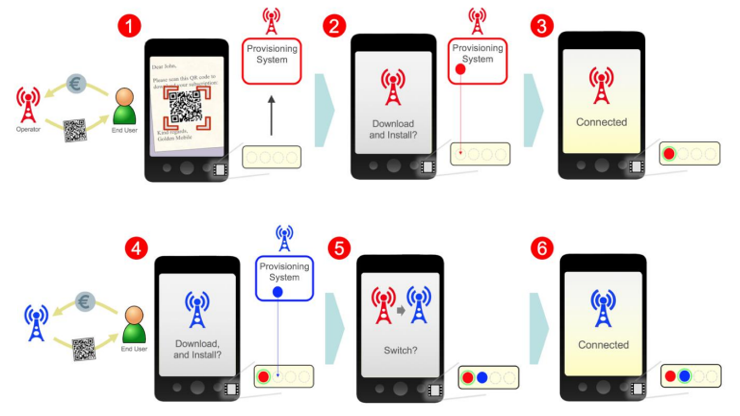
\includegraphics[width=\linewidth]{RSP-functioning.png}
\caption{Comunicazione tra end user e operatore nel contesto del Remote SIM Provisioning.}
\label{fig:RSP-functioning}
\end{figure}
\\Per quanto riguarda l'architettura interna di RSP nello specifico, esistono due soluzioni diverse \cite{GSMA-docs-new}.
\begin{enumerate}
\item \textbf{LPA embeddato nel dispositivo mobile ma non all'interno dell'eUICC (LPAd)}: oltre alla comunicazione tra l'applicazione LPA e SM-DP+, si utilizzano delle apposite interfacce anche per la comunicazione tra l'eUICC e l'applicazione LPA, come mostrato nella figura \ref{fig:RSP-LPAd} tratta da \cite{GSMA-docs-new}.
\begin{figure}
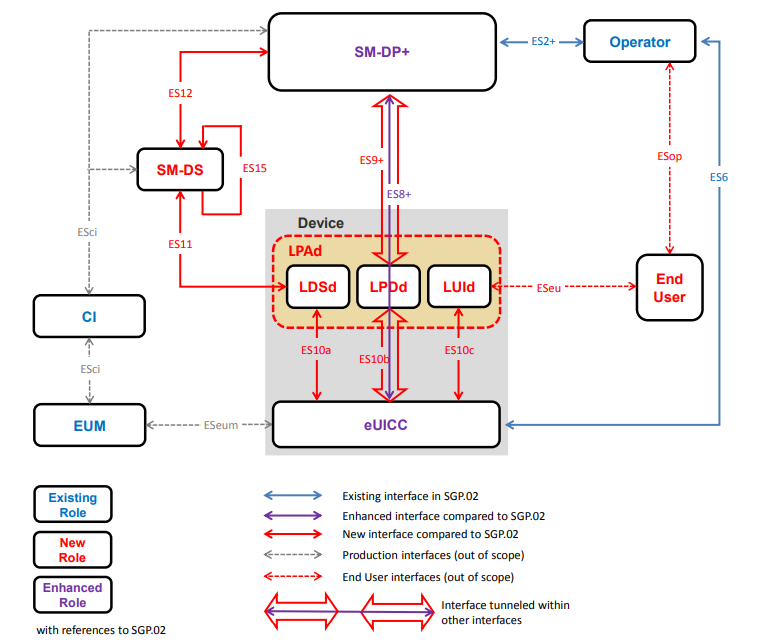
\includegraphics[width=\linewidth]{RSP-LPAd.png}
\caption{Architettura di RSP nel caso di LPA non embeddato nell'eUICC.}
\label{fig:RSP-LPAd}
\end{figure}
Di seguito è riportato un breve glossario che chiarisce il significato di alcuni componenti appartenenti all'architettura di RSP raffigurata in \ref{fig:RSP-LPAd}.
\begin{itemize}
\item \textbf{CI} = Certificate Issuer: nota anche come eSIM CA RootCA, è un'entità autorizzata a rilasciare certificati digitali.
\item \textbf{Device App} = una qualunque applicazione installata nel dispositivo mobile.
\item \textbf{Enterprise} = impresa (i.e. azienda, organizzazione o entità governativa) che si iscrive ai servizi mobili che devono essere utilizzati dai dipendenti a supporto dell'impresa stessa.
\item \textbf{EUM} = eUICC Manufacturer: è il fornitore delle eUICC e del software residente (e.g. firmware, sistema operativo); svolge anche il ruolo di certificate authority subordinata al CI e rilascia certificati all'eUICC \cite{GSMA-docs-new}\cite{Sec-analysis}.
\item \textbf{HRI Server} = server che fornisce le High Resolution Icon, che sono icone che vengono create per essere visualizzate in alta risoluzione.
\item \textbf{LDSd} = Local Discovery Service (quando l'LPA non è nell'eUICC).
\item \textbf{LPDd} = Local Profile Download (quando l'LPA non è nell'eUICC).
\item \textbf{LUId} = Local User Interface (quando l'LPA non è nell'eUICC).
\item \textbf{SM-DS} = Subscription Manager Discovery Server: è il componente che consente a SM-DP+ di raggiungere l'eUICC senza dover sapere a quale rete il dispositivo è connesso.
\end{itemize}
\item \textbf{LPA embeddato all'interno dell'eUICC (LPAe)}: sono necessarie solo delle interfacce tra l'eUICC e SM-DP+, come mostrato nella figura \ref{fig:RSP-LPAe} tratta da \cite{GSMA-docs-new}.
\begin{figure}
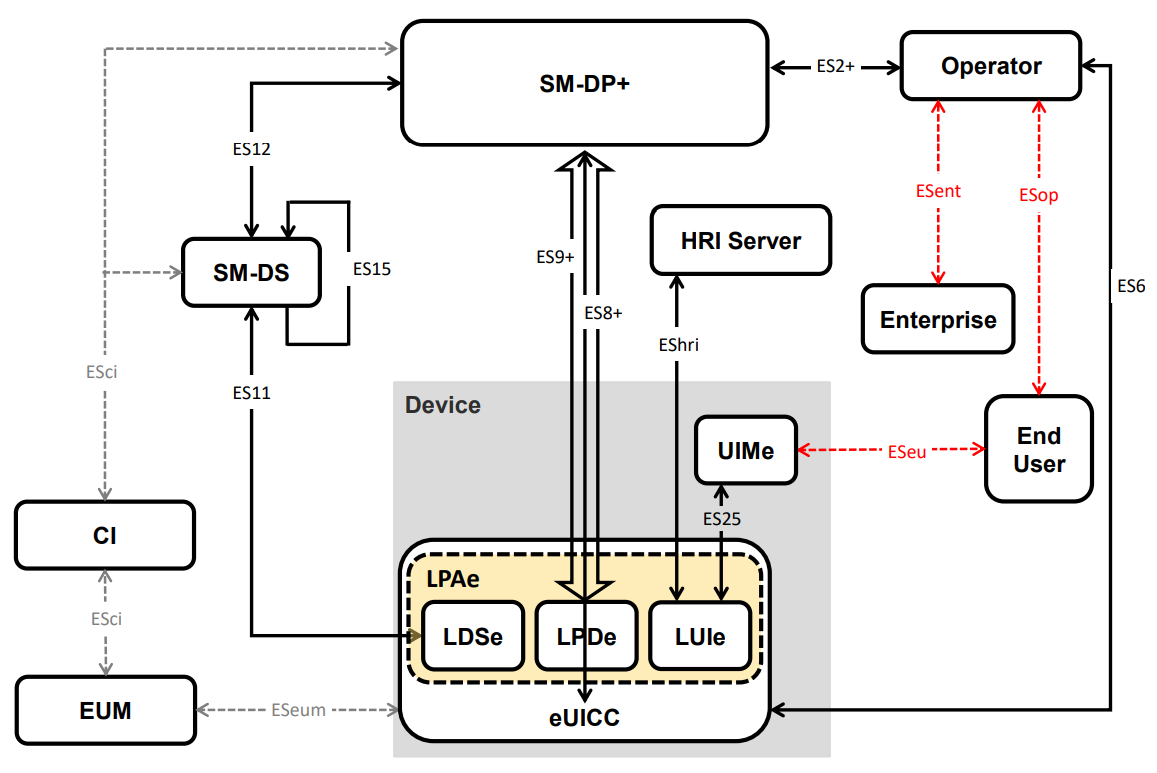
\includegraphics[width=\linewidth]{RSP-LPAe.png}
\caption{Architettura di RSP nel caso di LPA embeddato nell'eUICC.}
\label{fig:RSP-LPAe}
\end{figure}
Successivamente è riportato un breve glossario che chiarisce il significato di alcuni componenti appartenenti all'architettura di RSP raffigurata in \ref{fig:RSP-LPAe}.
\begin{itemize}
\item \textbf{LDSe} = Local Discovery Service (quando LPA è nell'eUICC).
\item \textbf{LPDe} = Local Profile Download (quando LPA è nell'eUICC).
\item \textbf{LUIe} = Local User Interface (quando LPA è nell'eUICC).
\item \textbf{UIMe} = User Inteface Module.
\end{itemize}
\end{enumerate}

\subsection{Interfacce presenti nell'architettura di RSP}
Sono illustrate nella tabella \ref{tab:interfaces}, costruita a partire da informazioni tratte da \cite{GSMA-docs-new}.\\
\begin{table}[h!]
\begin{center}
\captionsetup{skip=4pt}
\caption{Interfacce in RSP.}
\label{tab:interfaces}
\begin{tabularx}{\textwidth}{|c|c|c|X|} % <-- Alignments: 1st column center, 2nd center and 3rd center, with vertical lines in between
\hline
\textbf{Interfaccia} & \textbf{Componente 1} & \textbf{Componente 2} & \textbf{Descrizione}\\
\hline
ES2+ & Operatore & SM-DP+ & Viene usata dall'operatore per invocare la preparazione del Profile Package*.\\
\hline
ES6 & Operatore & eUICC & Viene usata dall'operatore per gestire il contenuto dei profili.\\
\hline
ES8+ & SM-DP+ & eUICC & Fornisce un canale end-to-end sicuro tra SM-DP+ e l'eUICC per l'amministrazione dell'ISD-P** e del relativo profilo durante il download e l'installazione.\\
\hline
ES9+ & SM-DP+ & LPD & Viene usata per fornire trasporto sicuro tra SM-DP+ e LPD per la consegna del Profile Package.\\
\hline
ES10a & LDSd & eUICC & Viene usata da LPAd per ottenere gli indirizzi configurati dall'eUICC per Root SM-DS*** (gestione di una Discovery Request).\\
\hline
ES10b & LPDd & eUICC & Viene usata da LPAd per trasferire un Profile Package all'eUICC.\\
\hline
ES10c & LUId & eUICC & Viene usata da LPAd per la gestione locale dei profili installati sull'eUICC da parte dell'end user (e.g. Enable, Disable, Delete).\\
\hline
ES11 & LDS & SM-DS & Viene usata per l'ottenimento di eventi.\\
\hline
ES12 & SM-DP+ & SM-DS & Viene usata per la gestione degli eventi.\\
\hline
ES15 & SM-DS & SM-DS & Viene usata per connettere gli SM-DS tra loro nel caso in cui ce ne sia più di uno.\\
\hline
ES22 & LPAd & Device App & Viene usata da un'applicazione del dispositivo mobile per interoperare con l'LPA.\\
\hline
ES25 & UIMe & LUIe & Viene usata per trasferire verso l'LPA le interazioni dell'end user.\\
\hline
ESop & Operatore & End user & È specifica per le relazioni di business tra l'operatore e l'end user.\\
\hline
ESeu & End user & LUI & È specifica per le relazioni di business tra l'end user e la LUI.\\
\hline
ESeum & eUICC & EUM & È specifica per le relazioni di business tra l'eUICC e l'EUM.\\
\hline
ESci & CI & SM-DP+, SM-DS, EUM & Viene usata per richiedere certificati.\\
\hline
EShri & LUI & HRI Server & Viene usata per recuperare le High Resolution Icon.\\
\hline
ESent & Operatore & Enterprise & È un'interfaccia che prescinde dagli scopi del presente documento.\\
\hline
ESapp & Operatore & Device App & È un'interfaccia che prescinde dagli scopi del presente documento.\\
\hline
\end{tabularx}
\end{center}
\end{table}
\\\textit{*Un Profile Package è un pacchetto di dati associato a un profilo che contiene le informazioni di configurazione necessarie per attivare e utilizzare quel profilo all'interno di una scheda eSIM. Esistono diversi tipi di Profile Package: l'Unprotected Profile Package (UPP) è un pacchetto di dati non protetto da alcun meccanismo di sicurezza; il Protected Profile Package (PPP) è un pacchetto di dati protetto da alcuni meccanismi di sicurezza, come l'autenticazione e/o la crittografia; il Bound Profile Package (BPP) è un pacchetto di dati legato a un particolare dispositivo o a una piattaforma di servizi; il Segmented Bound Profile Package (SBPP), infine, non è altro che un BPP suddiviso in molteplici segmenti che possono essere utilizzati in modo indipendente e separato.}\\ \\
\textit{**ISD-P (Issuer Security Domain Profile) è un contenitore sicuro che ospita un unico profilo.}\\ \\
\textit{***Root SM-DS è il server primario utilizzato da un operatore di rete mobile per gestire le attivazioni e le disattivazioni delle sottoscrizioni e per gestire funzionalità come l'autenticazione e l'autorizzazione degli utenti. D'altra parte, si hanno gli Alternative SM-DS, che sono server di backup a cui si ricorre quando il Root SM-DS non è disponibile.}

\section{Architettura dell'eUICC}
Nella figura \ref{fig:eUICC-arch} tratta da \cite{GSMA-docs-new} è schematizzata l'architettura interna del chip eUICC, dove i riquadri e le frecce in rosso sono relativi rispettivamente ai componenti e alle interfacce che, nell'ambito dell'eUICC, sono presenti esclusivamente nel caso in cui l'applicazione LPA sia effettivamente embeddata all'interno dell'eUICC (LPAe).
\begin{figure}
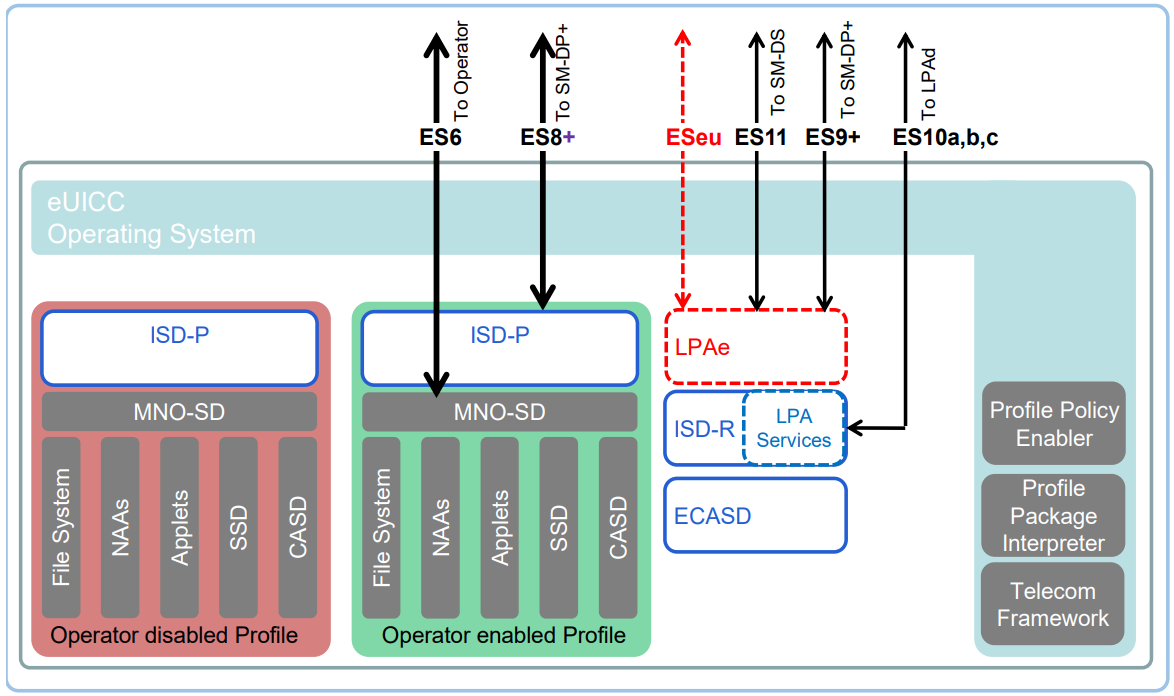
\includegraphics[width=\linewidth]{eUICC-arch.png}
\caption{Architettura dell'eUICC.}
\label{fig:eUICC-arch}
\end{figure}
\\Di seguito, invece, è riportato un breve glossario che chiarisce il significato di alcuni componenti appartenenti all'architettura dell'eUICC raffigurata in \ref{fig:eUICC-arch}.
\begin{itemize}
\item \textbf{CASD} = Controller Authority Security Domain: è un'area di storage sicura all'interno dell'ISD-P in cui vengono memorizzate le credenziali richieste (i.e. chiavi, certificati) per supportare le funzionalità di sicurezza sensibili.
\item \textbf{ECASD} = Embedded Controller Authority Security Domain: è il componente CASD direttamente incapsulato all'interno dell'eUICC.
\item \textbf{ISD-R} = Issuer Security Domain Root: è il componente responsabile della creazione di nuovi ISD-P e della gestione del loro ciclo di vita.
\item \textbf{LPA Services} = i seguenti quattro servizi: trasferimento del Bound Profile Package da LPAd all'ISD-P; ottenimento della lista dei profili installati; recupero dell'EID (eUICC ID); ottenimento delle operazioni di gestione del profilo locale (Local Profile Management Operations).
\item \textbf{MNO-SD} = Mobile Network Operator Security Domain: è la parte del profilo posseduta dall'operatore che fornisce all'operatore Over The Air (OTA) un canale di comunicazione sicuro; viene usato per gestire il contenuto di un profilo una volta che è stato abilitato.
\item \textbf{NAAs} = Network Access Applications: sono le applicazioni che consentono l'accesso alla rete.
\item \textbf{Profile Package Interpreter} = servizio del sistema operativo dell'eUICC che traduce i dati del Profile Package in un profilo installato all'interno dell'ISD-P usando il formato interno dell'eUICC.
\item \textbf{Profile Policy Enabler} = componente che verifica che il profilo eSIM possa essere installato sull’eUICC.
\item \textbf{SSD} = Supplementary Security Domain: è un'area di memoria protetta all'interno dell'ISD-P che viene utilizzata per l'esecuzione di funzioni di sicurezza come le operazioni crittografiche. Di fatto, il suo scopo principale è quello di proteggere le informazioni riservate dell'utente (i.e. chiavi, password) da accessi non autorizzati e attacchi esterni.
\item \textbf{Telecom Framework} = servizio del sistema operativo dell'eUICC che fornisce algoritmi di autenticazione di rete standardizzati alle applicazioni NAAs ospitate nei rispettivi ISD-P.
\end{itemize}

\subsection{Caratteristiche hardware e software dell'eUICC}
\begin{enumerate}[itemsep=0pt]
\item Deve essere resistente al tampering (manomissione) dei componenti hardware.
\item Contiene un unico ECASD (eUICC Controlling Authority Security Domain).
\item Supporta SHA-1.
%\item Supporta TUAK, che è un particolare algoritmo crittografico di 3GPP, dove 3GPP (Third Generation Partnership Project) è il consorzio industriale che definisce gli standard per la tecnologia 5G .
\item Supporta Milenage, che è un set di funzioni di autenticazione e di generazione di chiavi.
\item Tutte le funzioni crittografiche devono essere resistenti al tampering e agli attacchi side-channel.
\end{enumerate}

\section{Chiavi crittografiche e certificati}
\subsection{Chiavi crittografiche}\label{sec:keys}
I principali attori che interagiscono nel protocollo RSP sono l'eUICC, l'LPA e il server SM-DP+. Le chiavi utilizzate da loro hanno tutte un nome di tipo $<$XX$>$.$<$YY$>$.$<$ZZ$>$ \cite{GSMA-docs-new}, dove:
\begin{itemize}
\item \textbf{$<$XX$>$}: indica la natura della chiave (i.e. chiave pubblica PK, chiave privata SK, chiave pubblica one-time otPK, chiave privata one-time otSK).
\item \textbf{$<$YY$>$}: indica il proprietario della chiave.
\item \textbf{$<$ZZ$>$}: indica l'utilizzo della chiave (i.e. digital signature SIG, key agreement KA, TLS).
\end{itemize}
Le chiavi di maggiore rilievo, comunque sia, sono riportate nella tabella \ref{tab:keys} tratta da \cite{GSMA-docs-old}.
\begin{table}[h!]
\begin{center}
\captionsetup{skip=4pt}
\caption{Chiavi crittografiche in RSP.}
\label{tab:keys}
\begin{tabularx}{\textwidth}{|c|X|}
\hline
\textbf{Nome} & \textbf{Descrizione}\\
\hline
PK.EUICC.SIG & Chiave pubblica dell'eUICC usata per verificare le signature dell'eUICC. È inclusa nel certificato CERT.EUICC.SIG.\\
\hline
SK.EUICC.SIG & Chiave privata dell'eUICC usata per generare le signature.\\
\hline
PK.DPauth.SIG & Chiave pubblica del server SM-DP+ usata per verificare le signature del server in fase di autenticazione. È inclusa nel certificato CERT.DPauth.SIG.\\
\hline
SK.DPauth.SIG & Chiave privata del server SM-DP+ usata per generare le signature per autenticarsi all'eUICC.\\
\hline
PK.DPpb.SIG & Chiave pubblica del server SM-DP+ usata per verificare le signature del server comprese nel BPP.  È inclusa nel certificato CERT.DPpb.SIG.\\
\hline
SK.DPpb.SIG & Chiave privata del server SM-DP+ usata per generare le signature per il binding dei profili.\\
\hline
PK.DSauth.SIG & Chiave pubblica del server SM-DS usata per verificare le signature di SM-DS in fase di autenticazione. È inclusa nel certificato CERT.DSauth.SIG.\\
\hline
SK.DSauth.SIG & Chiave privata del server SM-DS usata per generare le signature per autenticarsi all'eUICC.\\
\hline
PK.EUM.SIG & Chiave pubblica dell'EUM usata per verificare i certificati degli eUICC. È inclusa nel certificato CERT.EUM.SIG.\\
\hline
SK.EUM.SIG & Chiave privata dell'EUM usata per firmare i certificati degli eUICC.\\
\hline
PK.CI.SIG &  Chiave pubblica del CI usata per verificare i certificati dell'EUM, dei server SM-DS e del server SM-DP+.\\
\hline
SK.CI.SIG & Chiave privata del CI usata per firmare i certificati dell'EUM, dei server SM-DS e del server SM-DP+.\\
\hline
otPK.EUICC.KA & Chiave pubblica one-time dell'eUICC usata per il key agreement.\\
\hline
otSK.EUICC.KA & Chiave privata one-time dell'eUICC usata per il key agreement.\\
\hline
otPK.DP.KA & Chiave pubblica one-time del server SM-DP+ usata per il key agreement.\\
\hline
otSK.DP.KA & Chiave privata one-time del server SM-DP+ usata per il key agreement.\\
\hline
PK.DP.TLS & Chiave pubblica del server SM-DP+ usata per verificare le signature TLS del server. È inclusa nel certificato CERT.DP.TLS.\\
\hline
SK.DP.TLS & Chiave privata del server SM-DP+ usata per generare le signature TLS per autenticarsi all'LPA.\\
\hline
PK.DS.TLS & Chiave pubblica del server SM-DS usata per verificare le signature TLS di SM-DS. È inclusa nel certificato CERT.DS.TLS.\\
\hline
SK.DS.TLS & Chiave privata del server SM-DS usata per generare le signature TLS per autenticarsi all'LPA.\\
\hline
\end{tabularx}
\end{center}
\end{table}

\subsection{Certificati}\label{sec:certificates}
I certificati propri dei principali componenti che partecipano all'interazione data dal protocollo RSP sono riportati nella tabella \ref{tab:cert} tratta da \cite{GSMA-docs-new}.\\
\begin{table}[h!]
\begin{center}
\captionsetup{skip=4pt}
\caption{Certificati in RSP.}
\label{tab:cert}
\begin{tabularx}{\textwidth}{|c|X|X|}
\hline
\textbf{Nome} & \textbf{Descrizione} & \textbf{Note}\\
\hline
CERT.CI.SIG & Certificato GSMA CI & Viene firmato e rilasciato da se stesso.\\
\hline
CERT.CISubCA.SIG & Certificato GSMA CI subordinato & Se esiste, viene firmato e rilasciato dal CI root.\\
\hline
CERT.EUM.SIG & Certificato EUM & Viene firmato e rilasciato dal CI (root o subordinato).\\
\hline
CERT.EUMSubCA.SIG & Certificato EUM subordinato & Se esiste, viene firmato e rilasciato dall'EUM root.\\
\hline
CERT.DPSubCA.SIG & Certificato SM-DP+ intermediario & Viene firmato e rilasciato dal CI (root o subordinato).\\
\hline
CERT.DPauth.SIG & Certificato SM-DP+ per autenticarsi all'eUICC & Viene firmato e rilasciato dal SM-DP+ intermediario o dal CI (root o subordinato).\\
\hline
CERT.DPpb.SIG & Certificato SM-DP+ per rilasciare e firmare i profili eSIM & Viene firmato e rilasciato dal SM-DP+ intermediario o dal CI (root o subordinato).\\
\hline
CERT.DP.TLS & Certificato TLS di SM-DP+ & Viene firmato e rilasciato dal SM-DP+ intermediario o dal CI (root o subordinato).\\
\hline
CERT.DSSubCA.SIG & Certificato SM-DS intermediario & Viene firmato e rilasciato dal CI (root o subordinato).\\
\hline
CERT.DSauth.SIG & Certificato SM-DS & Viene firmato e rilasciato dal SM-DS intermediario o dal CI (root o subordinato).\\
\hline
CERT.DS.TLS & Certificato TLS di SM-DS & Viene firmato e rilasciato dal SM-DS intermediario o dal CI (root o subordinato).\\
\hline
CERT.EUICC.SIG & Certificato eUICC & Viene firmato e rilasciato dall'EUM (root o subordinato).\\
\hline
CERT.CA.SIG & Certificato di una qualunque CA pubblica & Può firmare e rilasciare certificati TLS.\\
\hline
\end{tabularx}
\end{center}
\end{table}
\\La figura \ref{fig:cert-chain} tratta da \cite{GSMA-docs-old} definisce uno schema riassuntivo della struttura originale della catena di certificati definita dalla Public Key Infrastructure (PKI) di RSP.\\
Attualmente, invece, la struttura della certificate chain è più complessa e introduce molteplici varianti differenti (i.e. presenza o meno di GSMA CI subordinati, presenza o meno di EUM subordinati, presenza o meno di SM-DP+ intermediari, presenza o meno di SM-DS intermediari). Di seguito, per semplicità, più porzioni distinte della catena verranno analizzate separatamente.
\begin{itemize}
\item Porzione della catena comprendente il CI, l'EUM e l'eUICC: è riportata nella figura \ref{fig:cert-chain-new1} tratta da \cite{GSMA-docs-new} e prevede quattro varianti differenti.
\begin{itemize}
\item \textbf{Variante O (originale)}: il CI root rilascia certificati per l'EUM root, il quale rilascia a sua volta certificati per l'eUICC.
\item \textbf{Variante A}: il CI root rilascia certificati per l'EUM root; l'EUM root rilascia certificati per l'EUM subordinato; l'EUM subordinato, infine, rilascia certificati per l'eUICC.
\item \textbf{Variante B}: il CI root rilascia certificati per il CI subordinato; il CI subordinato rilascia certificati per l'EUM root; l'EUM root, infine, rilascia certificati per l'eUICC.
\item \textbf{Variante C}: il CI root rilascia certificati per il CI subordinato; il CI subordinato rilascia certificati per l'EUM root; l'EUM root rilascia certificati per l'EUM subordinato; l'EUM subordinato, infine, rilascia certificati per l'eUICC.
\end{itemize}
\item Porzione della catena comprendente il CI e i certificati di tipo SIG di SM-DP+ e SM-DS: è riportata nella figura \ref{fig:cert-chain-new2} tratta da \cite{GSMA-docs-new} e prevede quattro varianti differenti.
\begin{itemize}
\item \textbf{Variante O (originale)}: il CI root rilascia direttamente i certificati CERT.DPauth.SIG, CERT.DPpb.SIG, CERT.DSauth.SIG.
\item \textbf{Variante A}: il CI root rilascia certificati per l'SM-DP+ intermediario e l'SM-DS intermediario; l'SM-DP+ intermediario rilascia a sua volta i certificati  CERT.DPauth.SIG, CERT.DPpb.SIG; l'SM-DS intermediario rilascia il certificato CERT.DSauth.SIG.
\item \textbf{Variante B}: il CI root rilascia certificati per il CI subordinato, il quale rilascia a sua volta i certificati CERT.DPauth.SIG, CERT.DPpb.SIG, CERT.DSauth.SIG.
\item \textbf{Variante C}: il CI root rilascia certificati per il CI subordinato; il CI subordinato rilascia certificati per l'SM-DP+ intermediario e l'SM-DS intermediario; l'SM-DP+ intermediario rilascia i certificati CERT.DPauth.SIG, CERT.DPpb.SIG; l'SM-DS intermediario rilascia il certificato CERT.DSauth.SIG.
\end{itemize}
\item Porzione della catena comprendente il CI e i certificati TLS di SM-DP+ e SM-DS: è riportata nella figura \ref{fig:cert-chain-new3} tratta da \cite{GSMA-docs-new} e prevede quattro varianti differenti.
\begin{itemize}
\item \textbf{Variante O (originale)}: il CI root rilascia direttamente i certificati CERT.DP.TLS, CERT.DS.TLS.
\item \textbf{Variante A}: il CI root rilascia i certificati per l'SM-DP+ intermediario e l'SM-DS intermediario; l'SM-DP+ intermediario rilascia il certificato CERT.DP.TLS; l'SM-DS intermediario rilascia il certificato CERT.DS.TLS.
\item \textbf{Variante B}: il CI root rilascia certificati per il CI subordinato, il quale rilascia a sua volta i certificati CERT.DP.TLS, CERT.DS.TLS.
\item \textbf{Variante C}: il CI root rilascia certificati per il CI subordinato; il CI subordinato rilascia certificati per l'SM-DP+ intermediario e l'SM-DS intermediario; l'SM-DP+ intermediario rilascia il certificato CERT.DP.TLS; l'SM-DS intermediario rilascia il certificato CERT.DS.TLS.
\end{itemize}
\end{itemize}
Per quanto riguarda i certificati TLS, al posto del CI, può esserci come root qualunque CA pubblica, come mostrato nella figura \ref{fig:cert-chain-new4} tratta da \cite{GSMA-docs-new}. Anche con questa soluzione esistono diverse varianti.
\begin{itemize}
\item \textbf{Prima variante OO (originale)}: la CA pubblica root rilascia direttamente i certificati CERT.DP.TLS, CERT.DS.TLS.
\item \textbf{Seconda variante OO}: la CA pubblica root rilascia certificati per una catena di una o più CA pubbliche subordinate, l'ultima delle quali rilascia CERT.DP.TLS, CERT.DS.TLS.
\item \textbf{Prima variante AA}: la CA pubblica rilascia certificati per l'SM-DP+ intermediario e l'SM-DS intermediario; l'SM-DP+ intermediario rilascia il certificato CERT.DP.TLS; l'SM-DS intermediario rilascia il certificato CERT.DS.TLS.
\item \textbf{Seconda variante AA}: la CA pubblica rilascia certificati per una catena di una o più CA pubbliche subordinate; l'ultima CA pubblica subordinata rilascia certificati per l'SM-DP+ intermediario e l'SM-DS intermediario; l'SM-DP+ intermediario rilascia il certificato CERT.DP.TLS; l'SM-DS intermediario rilascia il certificato CERT.DS.TLS.
\end{itemize}
\begin{figure}
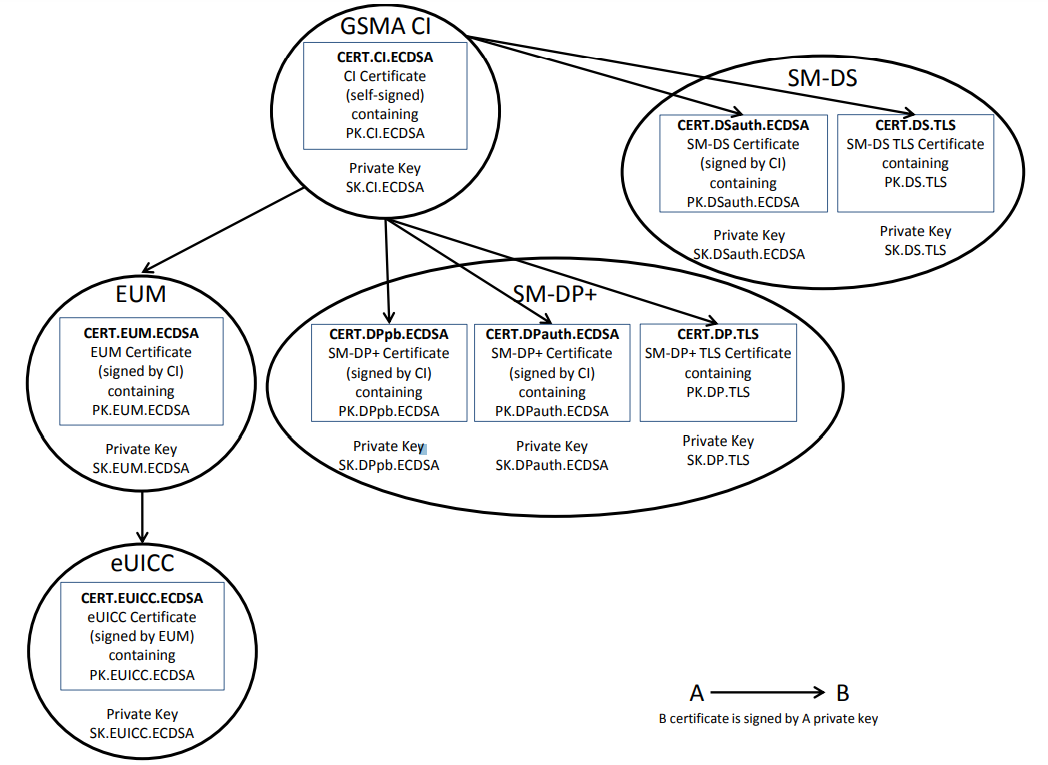
\includegraphics[width=\linewidth]{cert-chain.png}
\caption{Catena di certificati definita originariamente dalla PKI di RSP.}
\label{fig:cert-chain}
\end{figure}
\begin{figure}
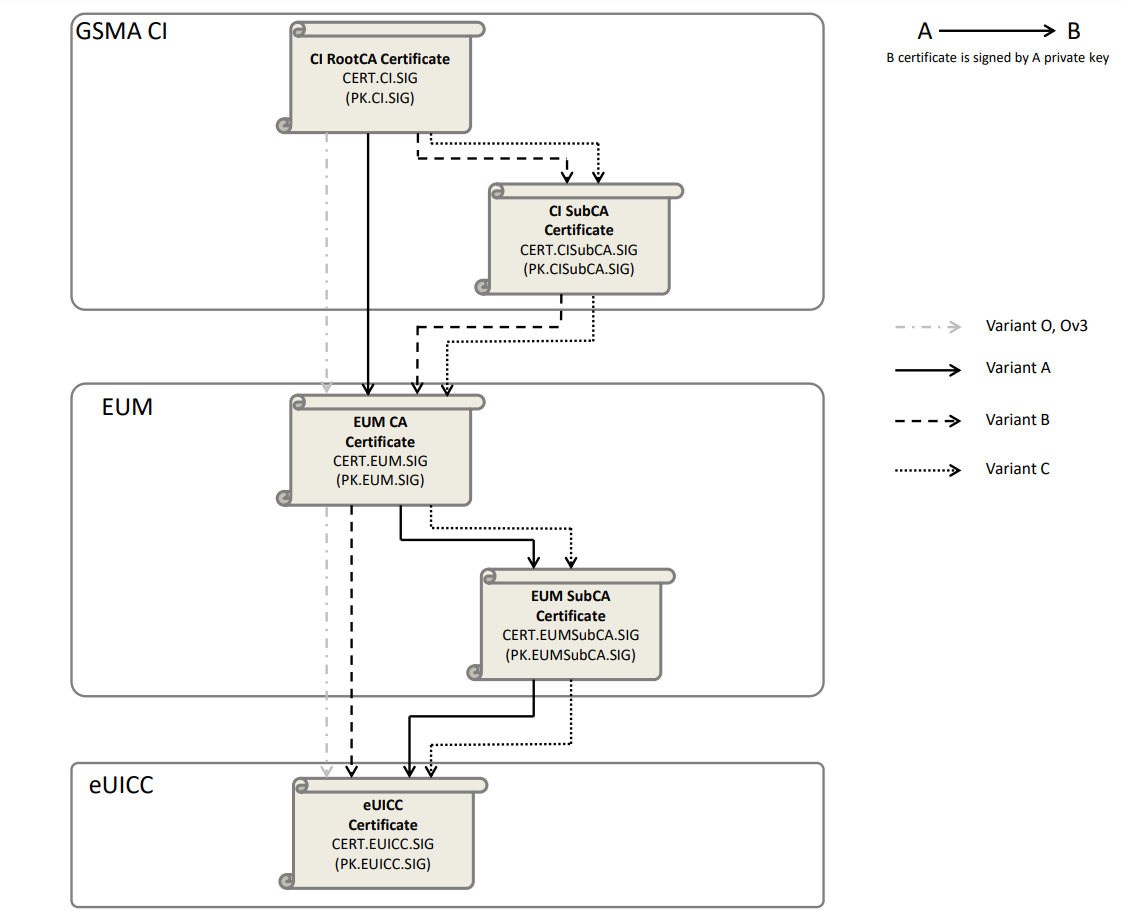
\includegraphics[width=\linewidth]{cert-chain-new1.png}
\caption{Prima porzione dell'attuale catena di certificati definita dalla PKI di RSP.}
\label{fig:cert-chain-new1}
\end{figure}
\begin{figure}
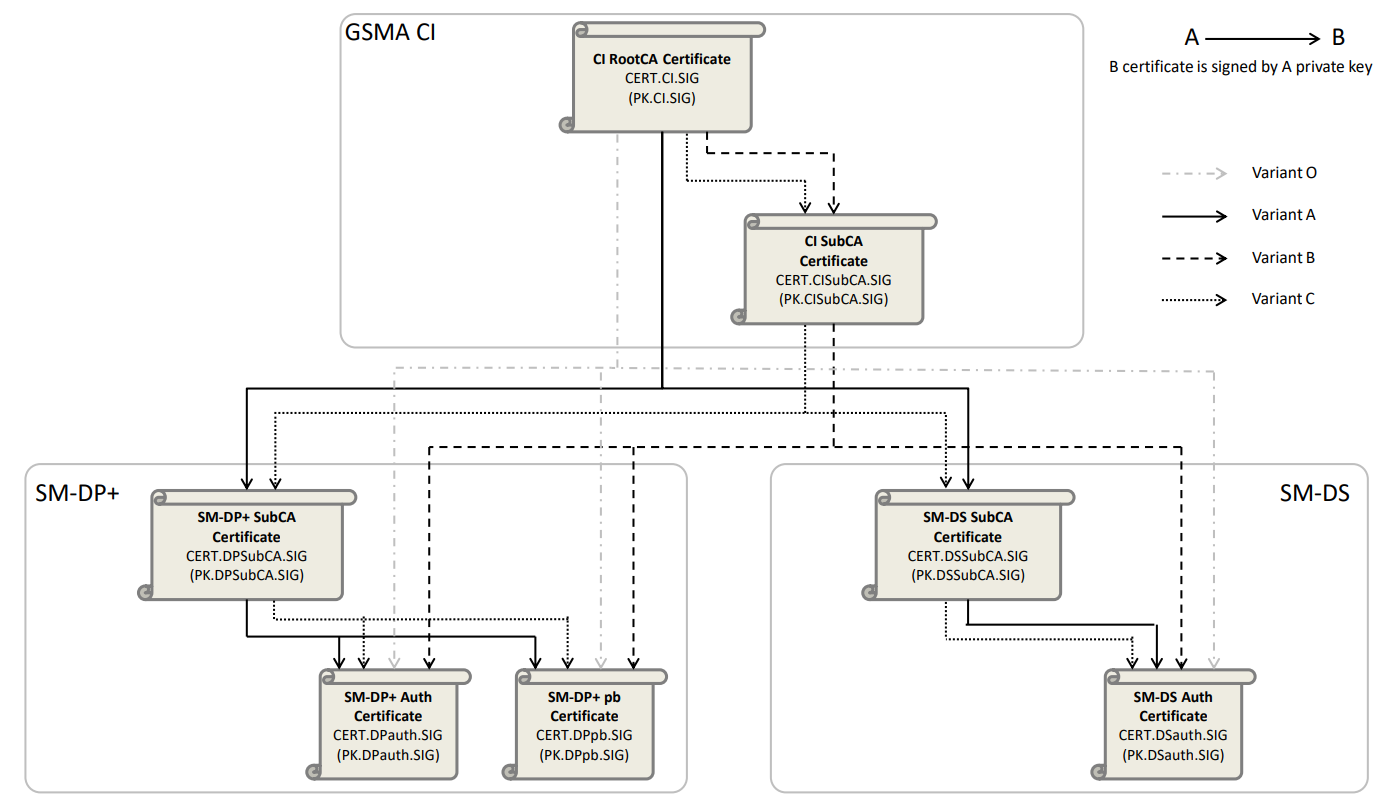
\includegraphics[width=\linewidth]{cert-chain-new2.png}
\caption{Seconda porzione dell'attuale catena di certificati definita dalla PKI di RSP.}
\label{fig:cert-chain-new2}
\end{figure}
\begin{figure}
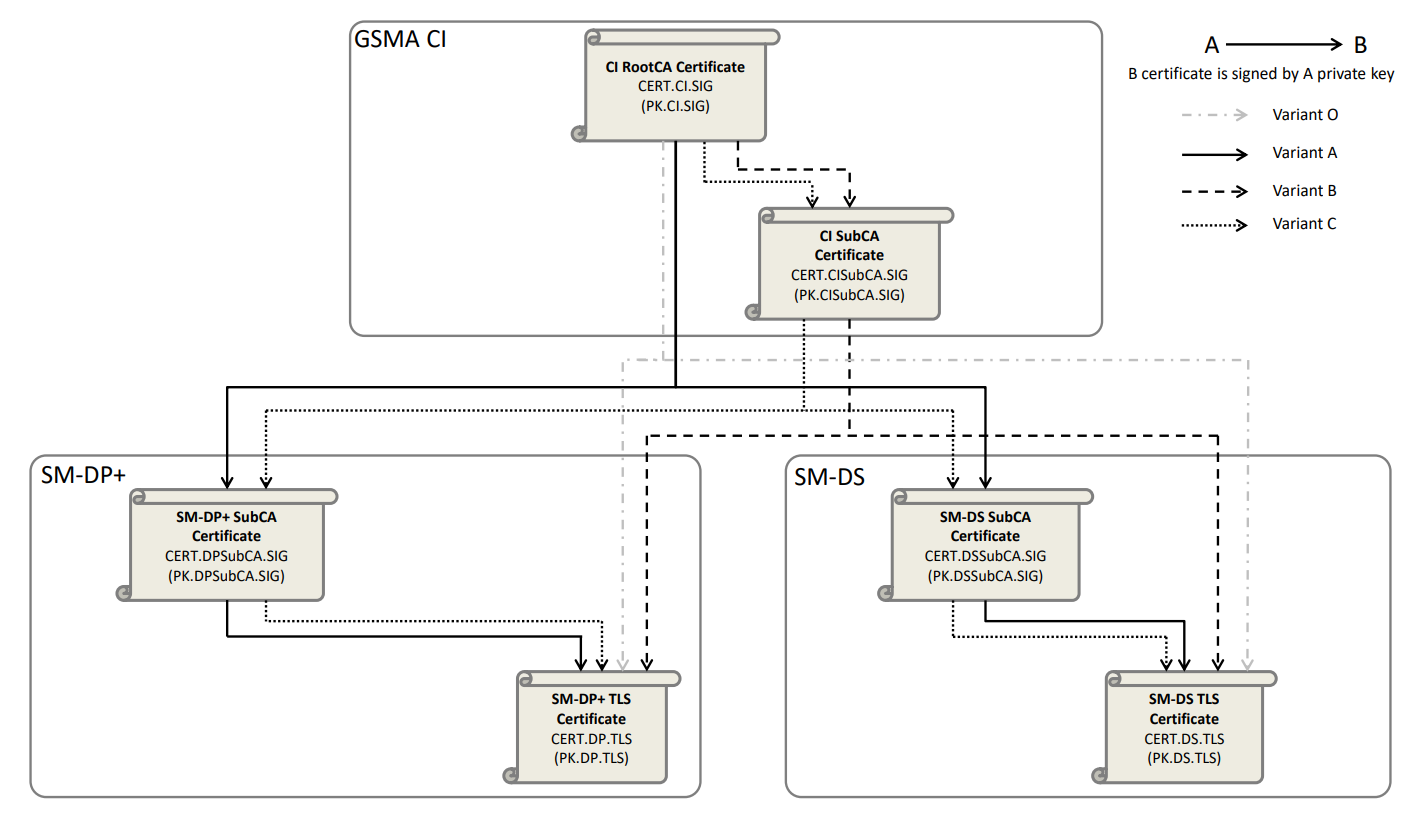
\includegraphics[width=\linewidth]{cert-chain-new3.png}
\caption{Terza porzione dell'attuale catena di certificati definita dalla PKI di RSP.}
\label{fig:cert-chain-new3}
\end{figure}
\begin{figure}
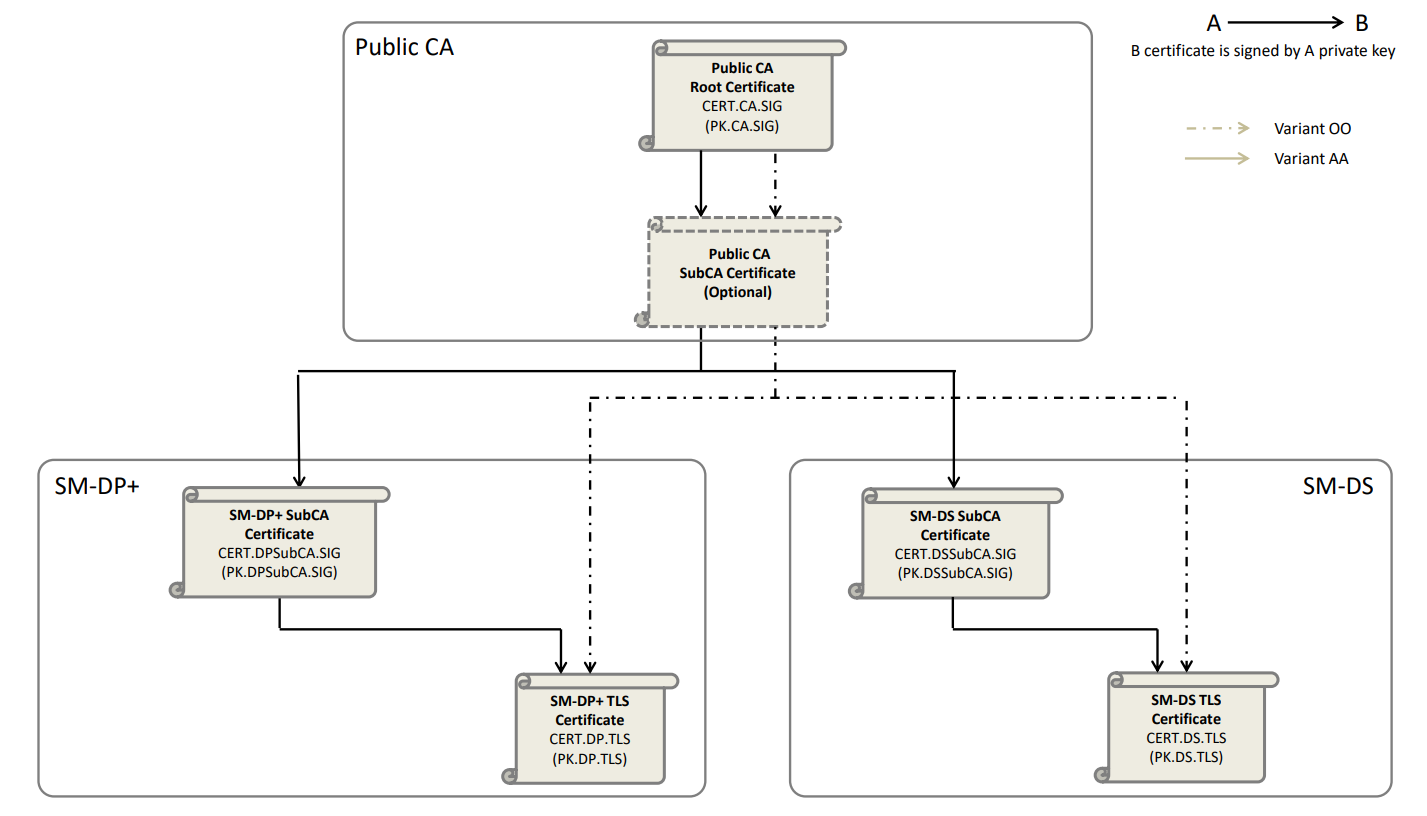
\includegraphics[width=\linewidth]{cert-chain-new4.png}
\caption{Quarta porzione dell'attuale catena di certificati definita dalla PKI di RSP.}
\label{fig:cert-chain-new4}
\end{figure}
All'interno della PKI, il Certificate Issuer di GSMA (CI) è la Root Certification Authority del servizio RSP e, di conseguenza, rappresenta il nodo radice della catena. Inoltre, tutti i certificati possono essere rilasciati direttamente dal CI (root o subordinato), fatta eccezione di CERT.EUICC.SIG che, invece, viene rilasciato dall'EUM (root o subordinato). Tutti i certificati che possono essere rilasciati direttamente dal CI hanno la possibilità di essere revocati in qualunque momento, in particolar modo se le entità corrispondenti (CI, EUM, SM-DP+, SM-DS) vengono compromesse. D'altra parte, i certificati eUICC (CERT.EUICC.SIG) non vengono revocati in modo individuale: di fatto, è difficile che un singolo eUICC venga compromesso. Piuttosto, è più verosimile che un modello eUICC o un intero batch di produzione di eUICC venga dichiarato come compromesso; quando ciò avviene, quello che si fa è revocare direttamente il certificato EUM (CERT.EUM.SIG) associato a quel modello o batch di produzione di eUICC \cite{GSMA-docs-new}.\\
Il CI fornisce una Certificate Revocation List (CRL), che è la lista dei certificati revocati tra tutti i certificati non scaduti che erano stati rilasciati da quello stesso CI. Ciascun CI, per giunta, deve pubblicare la propria CRL sia periodicamente, sia ogni volta che viene revocato un particolare certificato \cite{GSMA-docs-new}.\\
In realtà, i certificati relativi alla PKI di RSP di cui si è discusso finora non sono gli unici certificati utilizzati per effettuare il deployment dei profili eSIM: esiste anche un certificato per firmare l'applicazione LPA e un certificato da inserire in ciascun profilo eSIM da distribuire all'end user. Dove entrano in gioco tali certificati? Con riferimento alla guida di Android per le API e per l'implementazione del deployment dei profili eSIM \cite{Android-docs}, l'interazione tra un'applicazione LPA e l'interfaccia all'eUICC (legata al componente EuiccManager in \cite{Android-docs}) può avvenire solo se l'applicazione dispone dei privilegi dell'operatore. Di norma, tali privilegi sono conferiti all'applicazione se il certificato usato per firmarla coincide col certificato presente nel profilo fornito da SM-DP+.

\subsection{Aggiornamento delle chiavi pubbliche nell'eUICC}
L'eUICC può fornire un meccanismo per aggiornare il set di chiavi pubbliche memorizzate nell'ECASD dell'eUICC (che sono chiavi a lunga durata). L'implementazione di tale meccanismo è lasciata all'EUM o al produttore del dispositivo mobile e, stando alla guida ufficiale di GSMA \cite{GSMA-docs-new}, deve essere sicura. Tuttavia, nel momento in cui un'implementazione è affidata a terze parti, nessuno può garantire con certezza che la prescrizione sulla sicurezza venga rispettata, poiché non vengono seguite delle linee guida standard e consolidate.
%Di conseguenza, potrebbe essere utile approfondire mediante degli esperimenti pratici il funzionamento dell'aggiornamento del set di chiavi poste nell'ECASD e stabilire così se esiste qualche vulnerabilità da sfruttare a vantaggio di un attaccante.

\subsubsection{Contenuto dell'ECASD}
Tutti gli eUICC devono avere un ECASD che contenga \cite{GSMA-docs-new}:
\begin{itemize}[itemsep=0pt]
\item la chiave privata dell'eUICC (SK.EUICC.SIG);
\item il certificato dell'eUICC (CERT.EUICC.SIG) contenente la chiave PK.EUICC.SIG, che è la chiave pubblica dell'eUICC;
\item la chiave pubblica del CI root (PK.CI.SIG);
\item il certificato dell'EUM (CERT.EUM.SIG) e, opzionalmente, il certificato degli EUM subordinati (CERT.EUMSubCA.SIG);
\item un keyset dell'EUM per il rinnovo di chiavi e certificati.
\end{itemize}

\subsubsection{Quando avviene l'aggiornamento delle chiavi?}
La necessità di rinnovare le chiavi contenute nell'ECASD può presentarsi in due casi \cite{GSMA-docs-new}.
\begin{itemize}
\item L'applicazione LPA ha determinato che l'eUICC non supporta più il Public Key identificator (i.e. la rappresentazione in esadecimale dell'identificatore della chiave pubblica) del CI a capo delle chiavi contenute nell'ECASD.
\item Durante la procedura di Common Mutual Authentication, il server SM-DP+ ha restituito un certificato CERT.DPauth.SIG che ha come parent un Root Certificate non supportato dall'eUICC.
\end{itemize}

\section{Interazione tra eUICC, LPA, SM-DP+ e operatore}
\subsection{Sicurezza TLS}
Il protocollo TLS, la cui versione 1.2 è definita in RFC 5246 \cite{RFC-5246} e la cui versione 1.3 è definita in RFC 8446 \cite{RFC-8446}, è utilizzato per proteggere il traffico sulle interfacce ES2+ (tra server SM-DP+ e operatore) e ES9+ (tra server SM-DP+ e LPA), dove è prevista la mutua autenticazione tra le parti. La documentazione di GSMA di riferimento \cite{GSMA-docs-new} sottolinea l'obbligatorietà di fare uso di TLS v1.2 sia per gli algoritmi di autenticazione e autorizzazione, sia per l'integrità dei messaggi, sia per la confidenzialità. In realtà, introduce anche la possibilità (e suggerisce) di utilizzare TLS v1.3, che è la versione più recente di TLS e risolve le vulnerabilità che caratterizzano TLS v1.2, per cui, in linea di principio, dovrebbe risultare particolarmente difficoltoso da penetrare. Tuttavia, attualmente sembra essere solo un suggerimento, per cui in uno sviluppo futuro potrebbe essere interessante verificare quale sia la versione di TLS utilizzata per proteggere la comunicazione tra LPA e server SM-DP+.\\
Un discorso analogo vale per l'interazione che si ha nella mutua autenticazione tra l'eUICC e il server SM-DP+, dove le due parti interagiscono tra loro tramite un TLS tunnel \cite{Sec-analysis}. Per quanto invece riguarda la comunicazione tra eUICC e applicazione LPA, è richiesto l'utilizzo di un pairwise secure channel (ovvero di un canale di comunicazione sicuro rispetto alla confidenzialità e all'autenticazione dei messaggi) che collega le due parti all'interno del dispositivo mobile \cite{Sec-analysis}. Tuttavia, non esiste una specifica universale che imponga l'utilizzo di un particolare protocollo di crittografia per proteggere il pairwise secure channel, anche se il protocollo più utilizzato rimane TLS.
%Di nuovo, potrebbe essere una buona idea stabilire con un approccio pratico se nel canale di comunicazione tra eUICC e LPA viene utilizzato TLS oppure un protocollo differente.

\subsection{Regole per la comunicazione in RSP}
Qualunque comunicazione remota definita per il protocollo RSP deve far fede alle regole riportate di seguito \cite{GSMA-docs-new}.
\begin{itemize}
\item \textbf{Mutua autenticazione tra eUICC e server SM-DP+}: il server deve essere autenticato per primo da parte dell'eUICC, dove il processo di autenticazione deve includere la verifica di una catena di certificati del server. D'altra parte, l'eUICC deve essere autenticato in un secondo momento da parte del server, dove il processo di autenticazione, di nuovo, deve includere la verifica di una catena di certificati dell'eUICC; l'autenticazione dell'eUICC non si applica all'LPA.
\item \textbf{Privacy dei dati}: l'eUICC, in quanto client, non deve rivelare alcuna informazione privata a un server SM-DP+ non autenticato. Inoltre, non deve generare materiale firmato prima del completamento del processo di autenticazione del server.
\item \textbf{Protezione della comunicazione}: quando possibile, la comunicazione tra eUICC e server SM-DP+, oltre a essere protetta dall'integrità dei messaggi, dalla cifratura e dall'autenticazione del mittente, dovrebbe essere caratterizzata dalla proprietà di Perfect Forward Secrecy. Secondo tale proprietà, se anche una chiave a lungo termine viene compromessa, le chiavi di sessione generate a partire da essa rimangono comunque riservate.
\item \textbf{Autorizzazione}: il server SM-DP+ deve sempre verificare che il client che ha inviato una richiesta sia effettivamente autorizzato prima di far partire l'esecuzione della funzione desiderata.
\end{itemize}

\subsection{Step dell'interazione in RSP}\label{sec:step-RSP}
L'interazione tra le parti, nel contesto del protocollo RSP, avviene in quattro fasi distinte: profile ordering, download initialization, common handshake e profile download \cite{Sec-analysis}.
\begin{itemize}
\item \textbf{Profile ordering \& download initialization}: nella prima fase, l'operatore richiede al server SM-DP+ di preparare un profilo eSIM, e il server gli restituisce dei download initialization pointer (che possono essere rappresentati ad esempio da un codice di attivazione). Nella seconda fase, l'operatore consegna i download initialization pointer all'LPA in modo tale che poi sia possibile effettuare il download vero e proprio del profilo. Per questi primi due step, si possono seguire tre tipi di approcci differenti:
\begin{enumerate}
\item \underline{Default server approach}: la figura \ref{fig:default-server} tratta da \cite{Sec-analysis} mostra questo approccio. L'operatore (indicato con MNO - Mobile Network Operator) pre-condivide con l'eUICC l'indirizzo S del server. Quando vuole effettuare una nuova sottoscrizione e ottenere così un nuovo profilo, l'end user contatta l'operatore (messaggio 0), il quale ordina al server SM-DP+ il profilo per l'identificatore U dell'eUICC target (messaggio 1). Il server crea il nuovo profilo e lo invia all'operatore (messaggio 2), il quale notifica l'utente (messaggio 3). A tal punto, l'applicazione LPA viene avviata e, tramite un'operazione di get, recupera S dall'eUICC.
\item \underline{Activation Code approach}: la figura \ref{fig:activation-code} tratta da \cite{Sec-analysis} mostra questo secondo approccio. L'operatore ordina al server SM-DP+ dei profili (messaggio 1), e il server li rende disponibili con un codice di attivazione (tipicamente un codice QR) e li restituisce all'operatore (messaggio 2). Il codice di attivazione include l'indirizzo S del server, l'identificatore $I_{ac}$ del profilo e, opzionalmente, l'OID, ovvero l'identificatore del server SM-DP+. Quando l'end user vuole effettuare una nuova sottoscrizione e ottenere così un nuovo profilo, contatta l'operatore (messaggio 0, che può essere inviato sia prima che dopo l'interazione tra operatore e server SM-DP+ appena descritta), il quale restituisce il codice di attivazione opportuno (messaggio 3).
\item \underline{SM-DS assisted approach}: è un approccio analogo all'Activation Code, con la differenza che SM-DP+ si appoggia sui server SM-DS per comunicare con l'eUICC.
\end{enumerate}
\item \textbf{Common handshake}: questa fase, nota anche come Common Mutual Authentication, coinvolge tre attori fondamentali: il server SM-DP+, l'applicazione LPA e l'eUICC. I relativi dettagli sono riportati nella sezione \ref{sec:mutual-auth}.
\item \textbf{Profile download}: in quest'ultima fase, i cui dettagli sono riportati nella sezione \ref{sec:down-install}, viene calcolato uno shared secret da cui, mediante una key derivation function (KDF), saranno derivate le chiavi one-time di sessione k (per la cifratura) e k' (per l'integrità dei dati). Avviene poi il download del profilo eSIM, in cui il server SM-DP+ invia all'LPA il profilo cifrato con la chiave k e l'operatore di riferimento, dove entrambe le informazioni sono firmate singolarmente con la chiave k' mediante il meccanismo di message authentication code (MAC). Dopodiché, l'LPA mostra l'operatore all'utente, che dovrà stabilire se è corretto: se sì, l'LPA inoltra tutte le informazioni all'eUICC il quale, dopo aver derivato a sua volta le chiavi di sessione k, k', dovrà decriptare il profilo P, che risulterà finalmente essere utilizzabile.
\end{itemize}
\begin{figure}
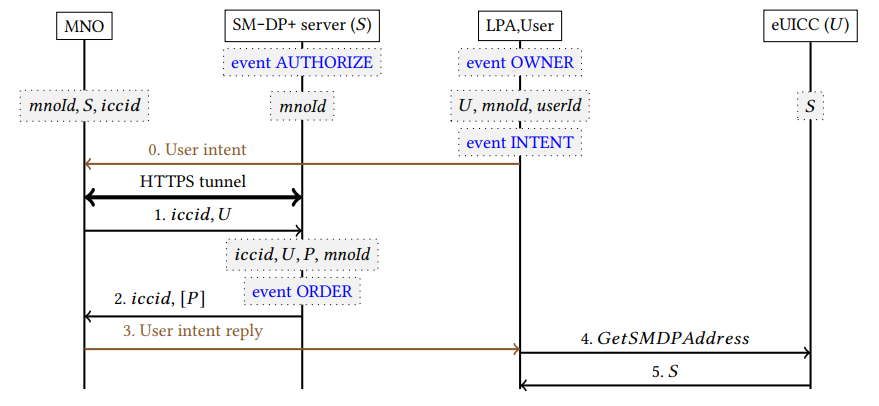
\includegraphics[width=\linewidth]{default-server.png}
\caption{Approccio default server per le fasi di profile ordering e download initialization.}
\label{fig:default-server}
\end{figure}
\begin{figure}
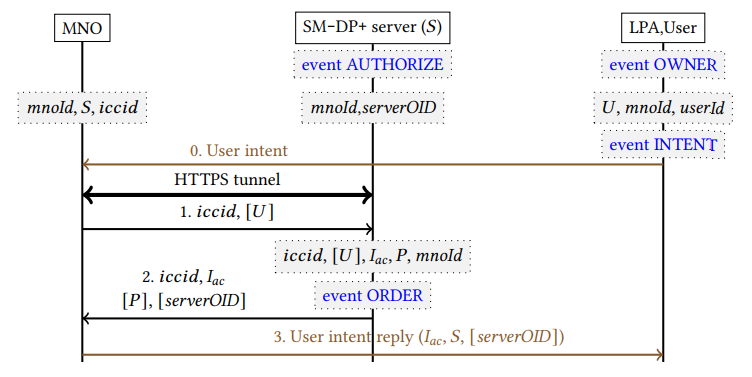
\includegraphics[width=\linewidth]{activation-code.png}
\caption{Approccio Activation Code per le fasi di profile ordering e download initialization.}
\label{fig:activation-code}
\end{figure}

\subsection{Ciclo di vita dei profili in SM-DP+}
Prima di approfondire più nel dettaglio l'interazione in RSP, è bene illustrare il ciclo di vita dei profili eSIM.\\
La tabella \ref{tab:profile-states} tratta da \cite{GSMA-docs-new}\cite{GSMA-docs-old} fornisce un elenco degli stati in cui ciascun profilo eSIM può trovarsi nell'arco della sua esistenza.
\begin{table}[h!]
\begin{center}
\captionsetup{skip=4pt}
\caption{Stati dei profili eSIM.}
\label{tab:profile-states}
\begin{tabularx}{\textwidth}{|c|X|}
\hline
\textbf{Nome} & \textbf{Descrizione}\\
\hline
Available & Il profilo è disponibile nell’inventory del server SM-DP+.\\
\hline
Allocated & Il profilo è riservato per il download senza essere linkato a un EID (eUICC ID).\\
\hline
Linked & Il profilo è riservato per il download ed è linkato a un EID.\\
\hline
Confirmed & Il profilo è riservato per il download (che sia esso linkato o non linkato a un EID) col Matching ID (i.e. il codice che identifica la transazione di download) e il codice di conferma (i.e. il codice che deve essere inserito dall'end user), se richiesti.\\
\hline
Released & Il profilo è pronto per il download e l’installazione dopo che l’operatore ha effettuato la configurazione di rete.\\
\hline
Downloaded & Il profilo è stato consegnato all’LPA (i.e. è stato scaricato).\\
\hline
Installed & Il profilo è stato installato sull’eUICC con successo.\\
\hline
Error & Il profilo non è stato installato a causa di una condizione di errore.\\
\hline
Unavailable & Il profilo non può essere più riutilizzato da SM-DP+.\\
\hline
\end{tabularx}
\end{center}
\end{table}
Nelle figure \ref{fig:profile-states1}, \ref{fig:profile-states2} tratte da \cite{GSMA-docs-new}\cite{GSMA-docs-old}, invece, sono mostrati due diagrammi a stati finiti che illustrano per bene il ciclo di vita dei profili in SM-DP+.
\begin{figure}
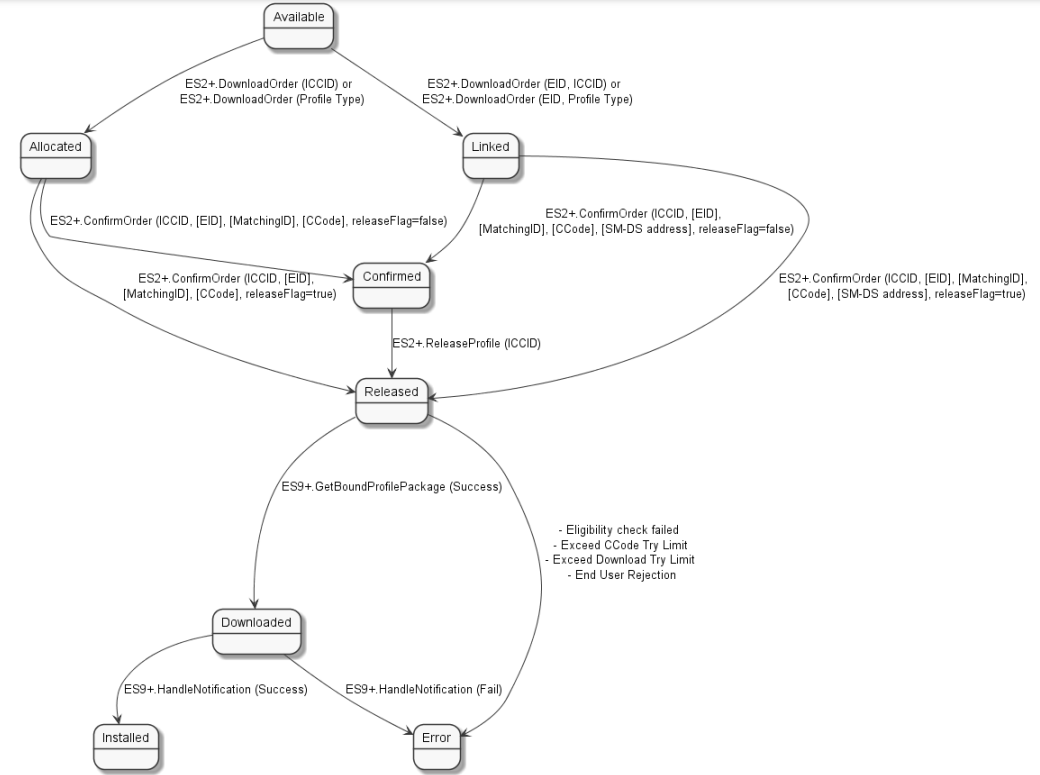
\includegraphics[width=\linewidth]{profile-states1.png}
\caption{Primo diagramma a stati per i profili eSIM.}
\label{fig:profile-states1}
\end{figure}
\begin{figure}
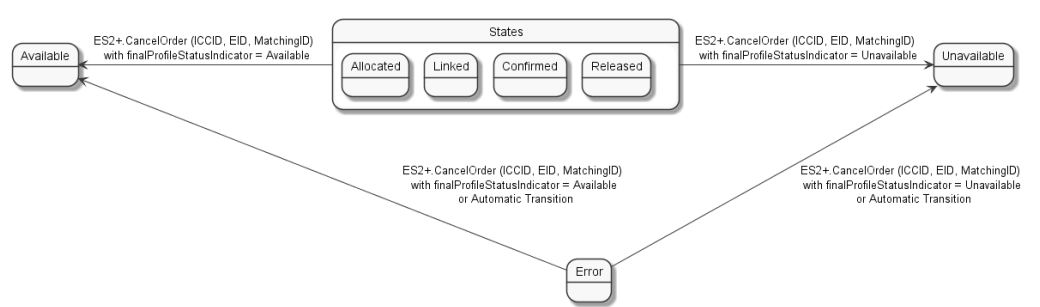
\includegraphics[width=\linewidth]{profile-states2.png}
\caption{Secondo diagramma a stati per i profili eSIM.}
\label{fig:profile-states2}
\end{figure}
\\
\\Con riferimento alla figura \ref{fig:profile-states1}, a partire dallo stato Available:
\begin{itemize}
\item Si passa allo stato Allocated se si effettua l'ordine di download senza specificare l'EID.
\item Si passa allo stato Linked se si effettua l'ordine di download specificando l'EID.
\end{itemize}
A partire dallo stato Allocated:
\begin{itemize}
\item Si passa allo stato Confirmed se si conferma l'ordine di download con releaseFlag=false.
\item Si passa allo stato Released se si conferma l'ordine di download con releaseFlag=true.
\end{itemize}
A partire dallo stato Linked:
\begin{itemize}
\item Si passa allo stato Confirmed se si conferma l'ordine di download con releaseFlag=false.
\item Si passa allo stato Released se si conferma l'ordine di download con releaseFlag=true.
\end{itemize}
A partire dallo stato Confirmed:
\begin{itemize}
\item Si passa allo stato Released se si effettua il rilascio del profilo in modo tale che sia effettivamente pronto per il download e l'installazione.
\end{itemize}
A partire dallo stato Released:
\begin{itemize}
\item Si passa allo stato Downloaded se il profilo viene consegnato all'LPA con successo.
\item Si passa allo stato Error se si ha un errore nel consegnare il profilo all'LPA.
\end{itemize}
A partire dallo stato Downloaded:
\begin{itemize}
\item Si passa allo stato Installed se il profilo viene installato sull'eUICC con successo.
\item Si passa allo stato Error se si ha un errore nell'installare il profilo sull'eUICC.
\end{itemize}
Con riferimento alla figura \ref{fig:profile-states2}, a partire dagli stati Allocated / Linked / Confirmed / Released:
\begin{itemize}
\item Si torna allo stato Available se l'ordine di download viene annullato con finalProfileStatusIndicator=Available.
\item Si passa allo stato Unavailable se l'ordine di download viene annullato con finalProfileStatusIndicator=Unavailable.
\end{itemize}
A partire dallo stato Error:
\begin{itemize}
\item Si torna allo stato Available con una transizione automatica oppure se l'ordine di download viene annullato con finalProfileStatusIndicator=Available.
\item Si passa allo stato Unavailable con una transizione automatica oppure se l'ordine di download viene annullato con finalProfileStatusIndicator=Unavailable.
\end{itemize}

\subsection{Dettagli sulla Common Mutual Authentication}\label{sec:mutual-auth}
La figura \ref{fig:common-mutual-auth} ripresa da \cite{GSMA-docs-new} illustra tutti i messaggi che il server SM-DP+, l'LPA e l'eUICC si scambiano tra loro e le operazioni che queste tre entità svolgono durante la procedura di Common Mutual Authentication. Tutti i relativi dettagli \cite{GSMA-docs-new} sono spiegati nelle sottosezioni successive. Si osservi che l'intero meccanismo resta valido e invariato se si ha un server SM-DS al posto del server SM-DP+.
\begin{figure}
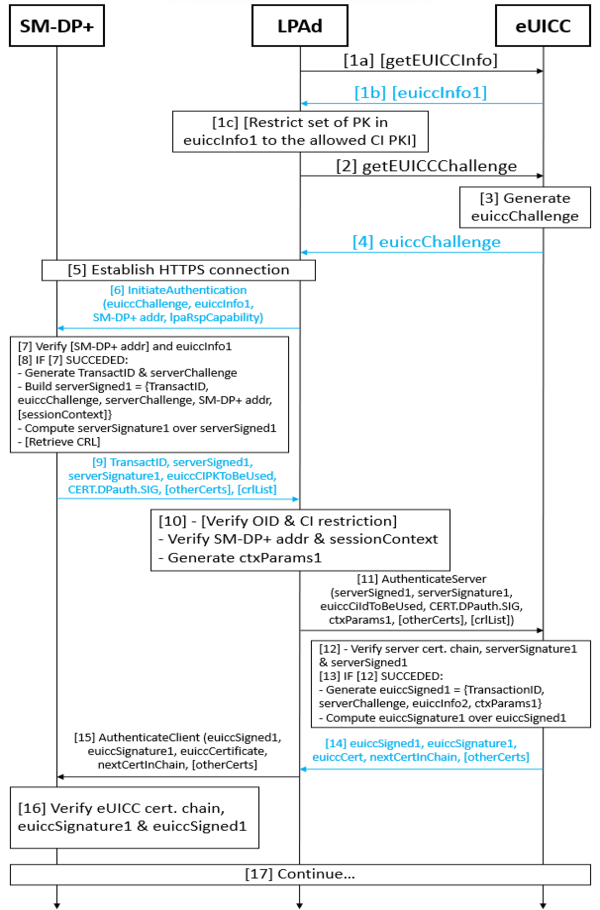
\includegraphics[width=\linewidth]{common-mutual-auth.png}
\caption{Sequence diagram che descrive la Common Mutual Authentication.}
\label{fig:common-mutual-auth}
\end{figure}

\subsubsection{Condizioni iniziali}
\begin{itemize}
\item Il server SM-DP+ è dotato di:
\begin{itemize}[itemsep=0pt]
\item certificato CERT.DPauth.SIG;
\item chiave privata SK.DPauth.SIG;
\item certificato del CI (CERT.CI.SIG);
\item certificato TLS CERT.DP.TLS;
\item chiave privata TLS SK.DP.TLS;
\item certificati di SM-DP+ intermediari, se esistenti (CERT.DPSubCA.SIG).
\end{itemize}
\item L'eUICC, d'altra parte, è dotato di:
\begin{itemize}[itemsep=0pt]
\item certificato CERT.EUICC.SIG;
\item chiave privata SK.EUICC.SIG;
\item certificato dell'EUM (CERT.EUM.SIG);
\item certificati di CI subordinati, se esistenti (CERT.CISubCA.SIG);
\item certificati di EUM subordinati, se esistenti (CERT.EUMSubCA.SIG);
\item chiave pubblica del CI (PK.CI.SIG).
\end{itemize}
\end{itemize}

\subsubsection{Procedimento}
\begin{enumerate}
\item Il primo step, che è opzionale, si articola in tre punti:
\begin{enumerate}[label=\alph*)]
\item Se non lo aveva già fatto in un momento precedente, l'LPA richiede le informazioni dell'eUICC (i.e. Specification Version Number e identificatori delle chiavi pubbliche del CI che possono essere utilizzate per autenticare il server e per firmare i propri dati) identificate dalla variabile euiccInfo1.
\item L'eUICC restituisce euiccInfo1 all'LPA.
\item Se esiste una restrizione sulle chiavi pubbliche consentite del CI, l'LPA crea una nuova istanza di euiccInfo1 senza le chiavi pubbliche non compatibili del CI. Se dopo questa operazione rimane una lista vuota di chiavi pubbliche, l'LPA informa l'end user che la procedura di mutua autenticazione deve terminare.
\end{enumerate}
\item L'LPA richiede all'eUICC una challenge (euiccChallenge).
\item L'eUICC genera la challenge che successivamente dovrà essere firmata dal server SM-DP+ per l'autenticazione del server stesso.
\item L'eUICC restituisce la challenge all'LPA.
\item L'LPA stabilisce una nuova connessione HTTPS col server SM-DP+. Il setup della sessione TLS, poiché non può riutilizzare le chiavi da una sessione precedente, deve prevedere un nuovo key exchange, che avviene nella fase del TLS handshake. Qui il server fornisce all'LPA un certificato CERT.DP.TLS e l'LPA deve verificarne la validità; se l'LPA non riesce a effettuare la verifica, il server deve inviargli un certificato CERT.DP.TLS differente, e così via, fin tanto che l'LPA non sarà riuscito a validare un certificato oppure il numero di tentativi per ritrasmettere il certificato non avrà raggiunto il limite massimo. In questo secondo caso l'LPA interrompe la procedura di Common Mutual Authentication.
\item L'LPA invoca la funzione \textit{InitiateAuthentication} passandovi come parametri le proprie capability, euiccChallenge, euiccInfo1 e l'indirizzo SM-DP+, il quale viene usato dall'LPA per accedere al server.
\item Il server SM-DP+ esegue le seguenti operazioni:
\begin{itemize}[itemsep=0pt]
\item Verificare che l'indirizzo SM-DP+ inviato dall'LPA sia valido.
\item Verificare il contenuto della variabile euiccInfo1, incluse le chiavi pubbliche del CI, tra cui deve essercene almeno una che può essere accettata dal server stesso.
\end{itemize}
Se anche solo uno di questi controlli non va a buon fine, il server restituisce una condizione di errore e l'LPA interrompe la procedura di Common Mutual Authentication.
\item Il server SM-DP+ esegue le seguenti altre operazioni:
\begin{itemize}[itemsep=0pt]
\item Generare un ID di transazione che serve per identificare la sessione RSP.
\item Generare una challenge (serverChallenge) che dovrà essere firmata dall'eUICC per l'autenticazione dell'eUICC stesso.
\item Generare una struttura dati serverSigned1 a partire dall'ID di transazione, da euiccChallenge, da serverChallenge, dall'indirizzo SM-DP+ ed eventualmente dal contesto di sessione.
\item Calcolare la serverSignature1 a partire da serverSigned1, utilizzando la chiave privata SK.DPauth.SIG.
\item Se sia l'eUICC che l'LPA prevedono il crlStaplingV3Support, che è la funzionalità che permette al server di fornire una Certificate Revocation List (CRL), il server deve anche recuperare la CRL per ciascun certificato che abbia l'estensione CRLDistributionPoints (i.e. per ciascun certificato che dà informazioni su dove è possibile ottenere una CRL).
\end{itemize}
\item Il server SM-DP+ restituisce all'LPA alcune informazioni, tra cui l'ID della transazione, serverSigned1, serverSignature1, euiccCIPKToBeUsed (che dovrà corrispondere alla chiave pubblica del CI accettata tra quelle proposte dall'eUICC), il certificato CERT.DPauth.SIG, eventuali altri certificati ed eventualmente la CRL.
\item L'LPA esegue le seguenti operazioni:
\begin{itemize}[itemsep=0pt]
\item Verificare l'OID, che è l'Object Identifier del server SM-DP+ (se fornito in precedenza).
\item Verificare che l'indirizzo SM-DP+ restituito dal server (incapsulato in serverSigned1) matchi con l'indirizzo SM-DP+ che l'LPA aveva inviato allo step (6).
\item Verificare che la chiave pubblica associata del Root della certificate chain associata al certificato CERT.DPauth.SIG sia inclusa in euiccInfo1 (se l'opzione euiccCiUpdateSupport dell'LPA è attiva).
\item Effettuare altre verifiche sui certificati che non verranno approfondite in questa sede.
\end{itemize}
Se anche solo uno di questi controlli non va a buon fine, l'LPA interrompe la procedura di Common Mutual Authentication. In caso contrario, procede col generare la struttura dati ctxParams1, che dovrà essere inviata all'eUICC affinché venga poi inclusa tra i dati firmati.
\item L'LPA invoca la funzione \textit{AuthenticateServer} passandovi come parametri serverSigned1, serverSignature1, euiccCiIdToBeUsed, il certificato CERT.DPauth.SIG, eventuali altri certificati, ctxParams1 ed eventualmente la CRL.
\item L'eUICC esegue le seguenti operazioni:
\begin{itemize}[itemsep=0pt]
\item Verificare il certificato CERT.DPauth.SIG e altri eventuali certificati nella catena.
\item Verificare serverSignature1.
\item Verificare che l'euiccChallenge contenuta in serverSigned1 matchi con la challenge generata dall'eUICC stessa allo step (3).
\item Verificare che la chiave pubblica del CI sia effettivamente supportata.
\item Se il contesto di sessione prevede il crlStaplingV3Support, l'eUICC deve anche verificare la validità della CRL e assicurarsi che nessun certificato all'interno della certificate chain sia stato revocato.
\end{itemize}
Se anche solo uno di questi controlli non va a buon fine, la procedura di Common Mutual Authentication deve essere interrotta. In caso contrario, il server SM-DP+ risulta autenticato all'eUICC.
\item L'eUICC esegue le seguenti altre operazioni:
\begin{itemize}[itemsep=0pt]
\item Generare la struttura dati euiccSigned1 a partire dall'ID di transazione, dall'indirizzo del server SM-DP+, da serverChallenge, da euiccInfo2 e da ctxParams1, dove euiccInfo2 è un sovrainsieme di euiccInfo1 e comprende le informazioni complete dell'eUICC. Si noti che euiccChallenge non è incluso in euiccSigned1.
\item Calcolare la euiccSignature1 a partire da euiccSigned1, utilizzando la chiave privata SK.EUICC.SIG.
\end{itemize}
\item L'eUICC restituisce all'LPA alcune informazioni, tra cui euiccSigned1, euiccSignature1 e la catena di certificati dell'eUICC.
\item L'LPA invoca la funzione \textit{AuthenticateClient} passandovi come parametri euiccSigned1, euiccSignature1 e la catena di certificati dell'eUICC.
\item Il server SM-DP+ esegue le seguenti operazioni:
\begin{itemize}[itemsep=0pt]
\item Verificare che l'ID di transazione contenuto in euiccSigned1 corrisponda a quello comunicato dal server stesso allo step (9).
\item Verificare che il certificato root della certificate chain comunicata dall'eUICC corrisponda con quella selezionata dal server stesso (euiccCIPKToBeUsed) durante l'esecuzione della funzione \textit{InitiateAuthentication}.
\item Verificare che la certificate chain dell'eUICC sia valida.
\item Verificare euiccSignature1.
\item Verificare che la serverChallenge contenuta in euiccSigned1 matchi con la challenge generata dal server stesso allo step (8).
\end{itemize}
Se anche solo uno di questi controlli non va a buon fine, il server restituisce una condizione di errore e l'LPA interrompe la procedura di Common Mutual Authentication. In caso contrario, l'eUICC risulta autenticato al server SM-DP+.
\end{enumerate}
In definitiva, in questa sezione è emerso come l'LPA svolga sì il ruolo di relay nell'interazione tra server SM-DP+ ed eUICC, ma svolge anche delle importanti funzioni di sicurezza. Infatti, com'è stato già menzionato, si occupa anzitutto di verificare che il certificato CERT.DP.TLS sia valido e, in un secondo momento, effettua altri controlli sull'OID, sull'indirizzo del server SM-DP+, sulla chiave pubblica associata al certificato CERT.DPauth.SIG e sulla certificate chain del server nello specifico. Tale caratteristica implica la necessità di considerare l'applicazione LPA come un'entità trusted.
%il che non è fortemente indicato dal punto di vista della sicurezza.

\subsection{Dettagli su download e installazione dei profili}\label{sec:down-install}
La figura \ref{fig:download-install} ripresa da \cite{GSMA-docs-new} illustra tutti i messaggi che l'operatore, il server SM-DP+, l'LPA e l'eUICC si scambiano tra loro e le operazioni che queste quattro entità svolgono durante la procedura di download e installazione dei profili. Tutti i relativi dettagli \cite{GSMA-docs-new} sono spiegati nelle sottosezioni successive. Anche qui l'intero meccanismo resta valido se si ha un server SM-DS al posto del server SM-DP+, a meno di variazioni di poco conto.
\begin{figure}
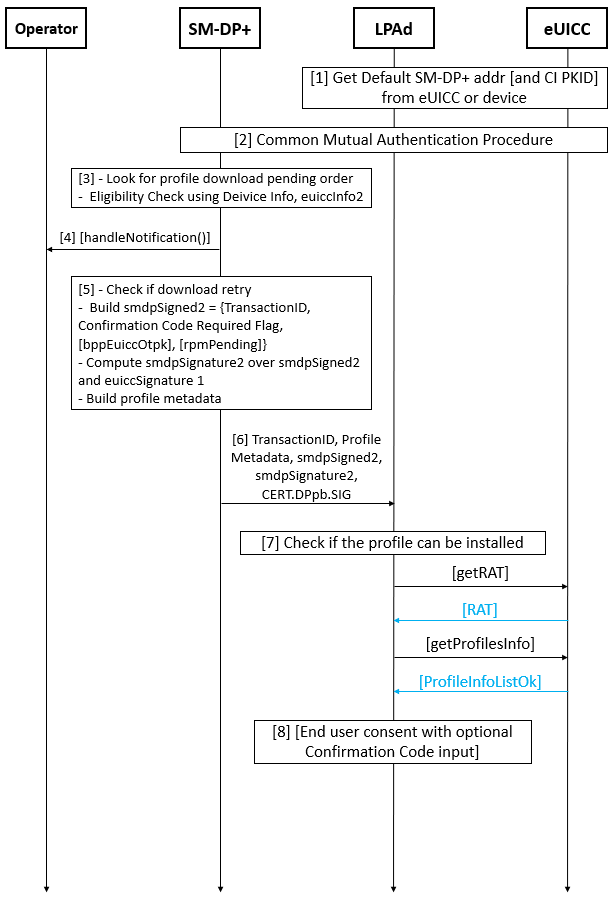
\includegraphics[width=\linewidth]{download-install.png}
\caption{Sequence diagram che descrive il download e l'installazione dei profili.}
\label{fig:download-install}
\end{figure}

\subsubsection{Condizioni iniziali}
\begin{itemize}
\item L'applicazione LPA potrebbe aver recuperato l'indirizzo del server SM-DP+ e l'identificativo della chiave pubblica del CI Root consentita; se tale identificativo viene effettivamente recuperato a partire dall'eUICC, allora l'LPA deve restringere l'insieme degli identificativi delle chiavi pubbliche dei CI Root compatibili a quel valore.
\item Per ogni profilo nello stato Released il server SM-DP+ mantiene un contatore dei tentativi di download di quel profilo e un contatore dei tentativi di immissione del codice di conferma. Di fatto, il server deve limitare il valore di questi due contatori.
\item Se è richiesto l'Activation Code per il download e l'installazione del profilo, l'end user deve averlo già immesso all'LPA.
\end{itemize}

\subsubsection{Procedimento}
\begin{enumerate}
\item Se non lo ha già fatto in precedenza e se è necessario, l'applicazione LPA effettua il parsing dell'Activation Code: così ottiene l'indirizzo del server SM-DP+ e, opzionalmente, l'OID del server SM-DP+ e l'identificativo della chiave pubblica del CI Root.
\item Viene eseguita la procedura di Common Mutual Authentication definita nella sezione \ref{sec:mutual-auth}. In particolare, nel messaggio \textit{AuthenticateClient}, l'LPA deve specificare il Matching ID, che è l'identificatore della transazione di download corrente e, dunque, individua esattamente il profilo che si vuole installare.
\item Il server SM-DP+ esegue le seguenti operazioni:
\begin{itemize}[itemsep=0pt]
\item Verificare che esista un profilo correlato al Matching ID ricevuto in \textit{AuthenticateClient}.
\item Se l'ordinazione di download del profilo è già linkato a un EID, verificare che quest'ultimo corrisponda all'EID dell'eUICC appena autenticato.
\item Verificare che il profilo sia nello stato Released o, nel caso di retry a seguito del fallimento di un'installazione precedente, nello stato Downloaded.
\end{itemize}
Se anche solo uno di questi controlli non va a buon fine, la procedura di download e installazione del profilo deve essere interrotta. In caso contrario, il server SM-DP+ deve procedere con le seguenti altre azioni:
\begin{itemize}[itemsep=0pt]
\item Incrementare il contatore dei tentativi di download del profilo target. Se il numero massimo di tentativi viene sforato, il server deve notificare l'operatore del fallimento del download e l'intera procedura deve terminare.
\item Effettuare i check di idoneità opportuni.
\end{itemize}
\item Il server SM-DP+ notifica l'operatore con l'esito dei check di validità mediante la funzione \textit{handleNotification} (step opzionale). La comunicazione tra server e operatore è protetta dall'uso di un pairwise secure channel, come nell'interazione tra eUICC e LPA; anche qui il protocollo più utilizzato è TLS ma non viene imposto dallo standard di GSMA. Di conseguenza, potrebbe essere nuovamente utile stabilire empiricamente se nel canale di comunicazione tra server SM-DP+ e operatore viene utilizzato TLS o meno.
\item Se i check di idoneità falliscono, allora il server SM-DP+ esegue le seguenti operazioni:
\begin{itemize}[itemsep=0pt]
\item Portare il profilo target allo stato Error.
\item Restituire uno status di errore all'LPA in modo tale che l'intera procedura termini.
\end{itemize}
In caso contrario, il server SM-DP+ esegue le seguenti altre operazioni:
\begin{itemize}[itemsep=0pt]
\item Determinare se è richiesto un codice di conferma (Confirmation Code) per l'ordinazione pendente.
\item Generare una struttura dati smdpSigned2 che contiene le proprie informazioni.
\item Calcolare smdpSignature2, che è un fingerprint ottenuto da smdpSigned2 ed euiccSignature1, dove euiccSignature1 è un'informazione che è stata scambiata durante la fase di Common Mutual Authetication.
\item Generare i metadati del profilo target.
\end{itemize}
\item Il server SM-DP+ fornisce all'LPA la risposta ad \textit{authenticateClient} (funzione invocata durante la procedura di Common Mutual Authentication), che comprende transactionId, i metadati del profilo, smdpSigned2, smdpSignature2 e CERT.DPpb.SIG.
\item L'LPA verifica se il profilo può essere effettivamente installato. Per far ciò, deve ricorrere a un'apposita struttura dati detta Rules Authorisation Table (RAT) e/o alla lista dei profili installati. Se non dispone già di queste informazioni, deve richiederle all'eUICC invocando le funzioni \textit{getRAT} e/o \textit{getProfilesInfo}. Informazioni più dettagliate sulla RAT e, più in generale, sulla gestione delle policy dei profili, sono riportate nella sezione \ref{sec:profile-policy}.
\item Se necessario, l'LPA richiede all'end user di inserire il codice di conferma che l'operatore gli aveva fornito. In caso contrario, l'LPA richiede una conferma semplice (Simple Confirmation) sul download del profilo, che può prevedere poche semplici opzioni di risposta come `Yes', `No', `Not now'. Se l'end user non inserisce correttamente il codice di conferma o non risponde positivamente alla conferma semplice, si procede con la cancellazione della sessione (Common Cancel Session Procedure, i cui dettagli sono riportati nella sezione \ref{sec:common-cancel-session}); altrimenti, l'installazione del profilo può completarsi con successo mediante la sotto-procedura di Download Confirmation, che verrà illustrata qui di seguito.
\end{enumerate}

\subsection{Sotto-procedura di Download Confirmation}\label{sec:down-confirm}
La figura \ref{fig:download-confirmation} ripresa da \cite{GSMA-docs-new} illustra tutti i messaggi che l'operatore, il server SM-DP+, l'LPA e l'eUICC si scambiano tra loro e le operazioni che queste quattro entità svolgono durante la sotto-procedura di Download Confirmation, che conclude la procedura di download e installazione dei profili introdotta poc'anzi. Tutti i relativi dettagli \cite{GSMA-docs-new} sono spiegati nelle sottosezioni successive. Ancora una volta i passaggi rimangono gli stessi se si ha un server SM-DS al posto del server SM-DP+.
\begin{figure}
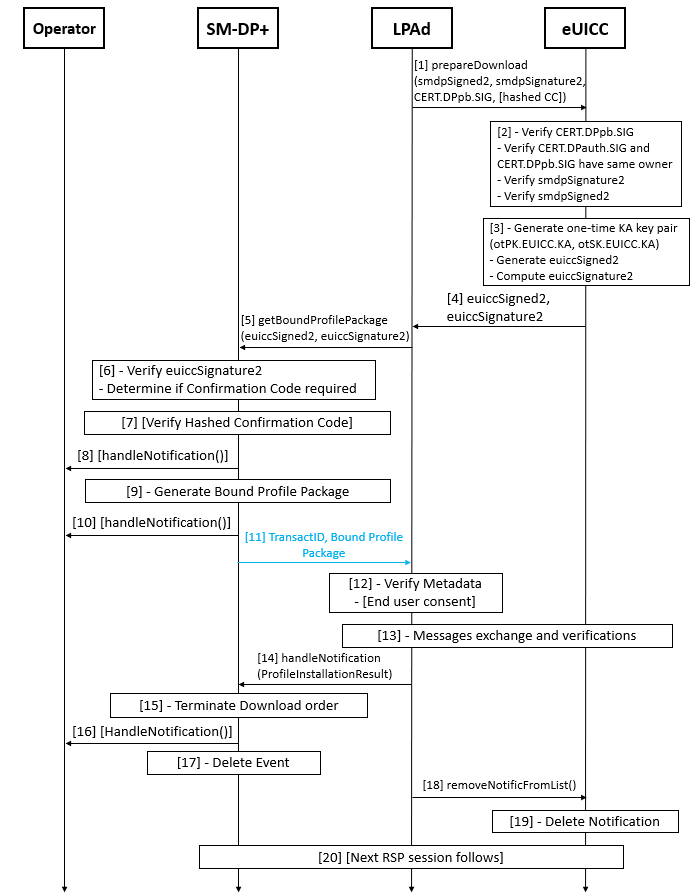
\includegraphics[width=\linewidth]{download-confirmation.png}
\caption{Sequence diagram che descrive la sotto-procedura di Download Confirmation.}
\label{fig:download-confirmation}
\end{figure}

\subsubsection{Condizioni iniziali}
\begin{itemize}
\item L'end user ha consentito con successo il download del profilo target.
\end{itemize}

\subsubsection{Procedimento}
\begin{enumerate}
\item L'LPA invoca la funzione \textit{prepareDownload} passandovi come parametri le informazioni precedentemente ricevute del server SM-DP+ (come smdpSigned2, smdpSignature2 e il certificato CERT.DPpb.SIG) e opzionalmente l'hash del codice di conferma (Confirmation Code).
\item L'eUICC esegue le seguenti operazioni:
\begin{itemize}[itemsep=0pt]
\item Verificare che CERT.DPpb.SIG sia un certificato valido.
\item Verificare che CERT.DPauth.SIG e CERT.DPpb.SIG appartengano alla medesima entità e siano state rilasciate dalla medesima CA.
\item Verificare smdpSignature2.
\item Verificare che l'ID di transazione contenuto in smdpSigned2 corrisponda con l'ID di transazione che identifica la sessione RSP corrente.
\end{itemize}
Se anche solo uno di questi controlli non va a buon fine, l'eUICC deve restituire uno stato di errore e la procedura di download e installazione del profilo deve essere interrotta. 
\item L'eUICC prosegue con le seguenti altre azioni:
\begin{itemize}[itemsep=0pt]
\item Generare una coppia di chiavi one-time (otPK.EUICC.KA, otSK.EUICC.KA).
\item Generare la struttura dati euiccSigned2, che comprende l'ID di transazione, la chiave pubblica one-time otPK.EUICC.KA ed eventualmente l'hash del Confirmation Code.
\item Calcolare euiccSignature2.
\end{itemize}
\item L'eUICC restituisce all'LPA la risposta a \textit{prepareDownload}.
\item L'LPA invoca la funzione \textit{getBoundProfilePackage} passandovi come parametri euiccSigned2 ed euiccSignature2.
\item Il server SM-DP+ verifica euiccSignature2 e stabilisce se è richiesto il codice di conferma: se sì, si procede con lo step (7), altrimenti si passa allo step (9).
\item Il server SM-DP+ esegue le seguenti operazioni:
\begin{itemize}[itemsep=0pt]
\item Recuperare l'hash del Confirmation Code ottenuto dalla funzione \textit{confirmOrder} relativa alle fasi di profile ordering \& download initialization, e calcolarne il valore atteso come SHA256(SHA256(Confirmation Code) $\vert$ transactionID).
\item Verificare che l'hash del Confirmation Code ricevuto all'interno di euiccSigned2 corrisponda col valore hash atteso.
\item Se la verifica dell'hash del Confirmation Code fallisce, incrementare di un'unità il contatore dei tentativi di immissione del codice e verificare che tale contatore non sfori il numero massimo ammissibile.
\end{itemize}
Se anche solo uno di questi controlli non va a buon fine, il server SM-DP+ deve restituire uno stato di errore e la procedura di download e installazione del profilo deve essere interrotta. Più precisamente, se fallisce il controllo sul contatore dei tentativi di immissione del codice di attivazione, è necessario anche impostare il profilo target nello stato Error e passare allo step (8) prima di interrompere la procedura. Se invece i controlli vanno tutti a buon fine, si passa allo step (9).
\item Se il numero di tentativi di immissione del codice di attivazione supera il massimo stabilito, il server SM-DP+ informa l'operatore del fallimento mediante la funzione \textit{handleNotification}; dopodiché, la procedura di download e installazione del profilo viene interrotta.
\item Il server SM-DP+ genera una coppia di chiavi one-time (otPK.DP.KA, otSK.DP.KA) da cui, assieme alla chiave otPK.EUICC.KA precedentemente ricevuta, ricava uno shared secret usato per cifrare e autenticare alcuni metadati del profilo da inviare al client; dopodiché, a partire da tali metadati e dal payload (cifrato) del profilo, genera il Bound Profile Package.
\item Il server SM-DP+ può opzionalmente notificare l'operatore del completamento del download del profilo mediante la funzione \textit{handleNotification}.
\item Il server SM-DP+ invia all'LPA la risposta a \textit{getBoundProfilePackage} e imposta lo stato del profilo target a Downloaded.
\item Se l'LPA ha già trattato la struttura dati Profile Metadata in precedenza, allora deve assicurarsi che le informazioni contenute nel Bound Profile Package (BPP) appena ricevuto le informazioni relative ai metadati del profilo siano rimaste coerenti; se non dovessero esserlo, deve avviare la Common Cancel Session Procedure (\ref{sec:common-cancel-session}) per cancellare la sessione corrente.
\item L'LPA e l'eUICC si scambiano una serie di messaggi per effettuare opportuni controlli e per portare a termine l'installazione del profilo all'interno dell'eUICC.
\item L'LPA invoca la funzione \textit{handleNotification} con lo scopo di consegnare il risultato dell'installazione del profilo al server SM-DP+, il quale risponderà con un semplice acknowledgement.
\item Il server SM-DP+ esegue le seguenti operazioni:
\begin{itemize}[itemsep=0pt]
\item Recuperare l'ordinazione di download del profilo target identificata dall'ID di transazione. Se viene ricevuto un ID di transazione ignoto, bisogna interrompere la procedura.
\item Chiudere l'ordinazione di download del profilo target e impostare il relativo stato a Installed o Error in base a quanto indicato dal risultato dell'installazione del profilo.
\end{itemize}
\item Eventualmente il server SM-DP+ invoca ancora una volta la funzione \textit{handleNotification} specificando l'esito dell'installazione del profilo sull'eUICC.
\item Se oltre al server SM-DP+ è coinvolto anche un SM-DS, allora il server SM-DP+ esegue la procedura di eliminazione dell'evento dall'SM-DS.
\item Alla ricezione dell'acknowledgement da parte del server SM-DP+, l'LPA invoca la funzione \textit{removeNotificationFromList} sull'eUICC.
\item L'eUICC cancella il risultato dell'installazione del profilo dalla propria memoria non volatile.
\item Se l'LPA aveva ricevuto rpmPending nel messaggio di risposta ad \textit{authenticateClient}, allora dovrebbe iniziare a una sessione RSP aggiuntiva col server SM-DP+, settando l'operationType a RPM (Remote Profile Management).
\end{enumerate}
%In definitiva, sembra che il modo più semplice per bucare la procedura di download e installazione dei profili sia sfruttare eventuali vulnerabilità presenti nella procedura di Common Mutual Authentication.

\subsection{Cambio di dispositivo}\label{sec:device-change}
La figura \ref{fig:device-change} ripresa da \cite{GSMA-docs-new} illustra tutti i messaggi che l'end user, l'LPA installata nel vecchio dispositivo, l'eUICC presente nel vecchio dispositivo, il server SM-DP+, l'LPA installata nel nuovo dispositivo, l'eUICC presente nel nuovo dispositivo e l'operatore (qui indicato come Service Provider) si scambiano tra loro e le operazioni che queste sette entità svolgono durante la procedura di trasferimento di un profilo dovuto al cambio di dispositivo. Tutti i relativi dettagli \cite{GSMA-docs-new} sono spiegati nelle sottosezioni successive.
\begin{figure}
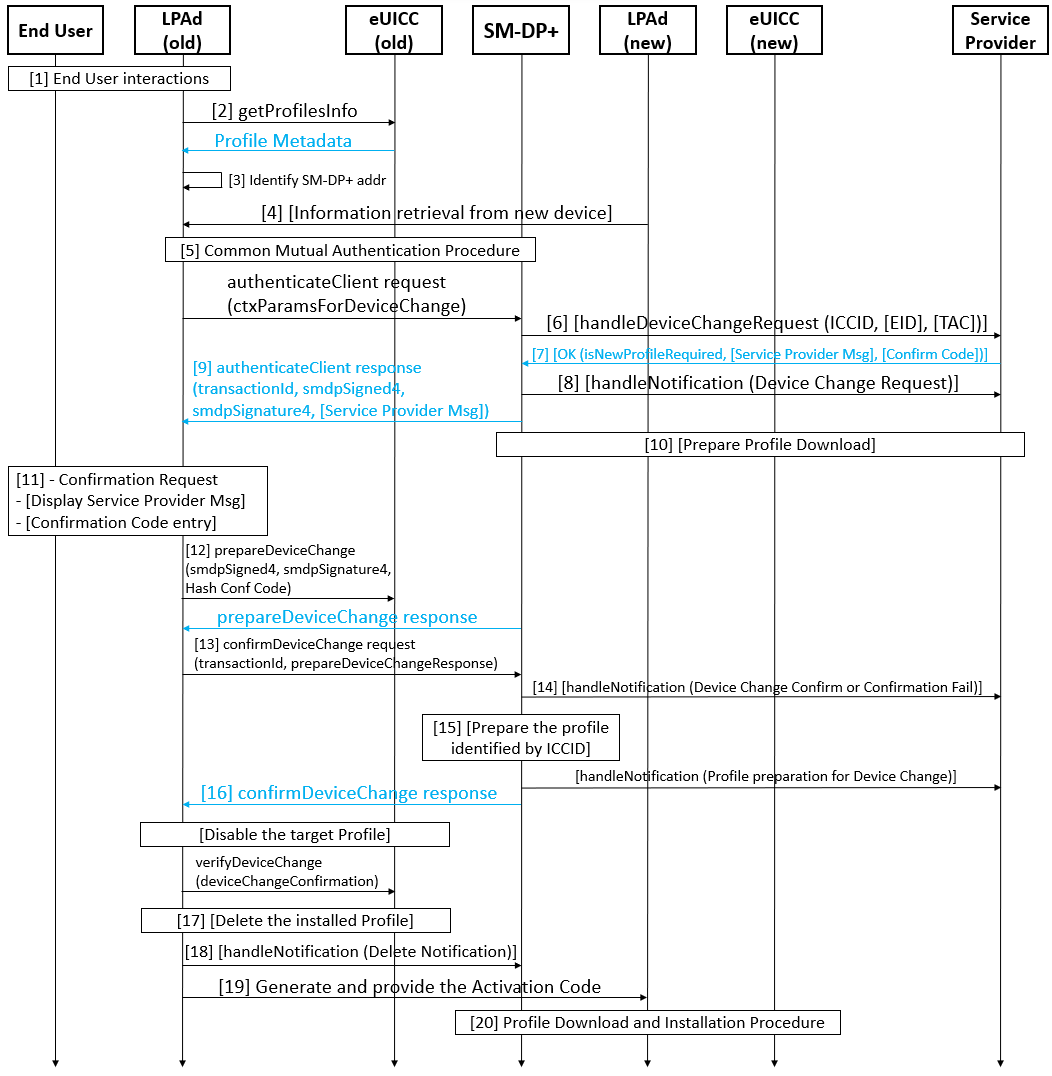
\includegraphics[width=\linewidth]{device-change.png}
\caption{Sequence diagram che descrive il trasferimento di un profilo.}
\label{fig:device-change}
\end{figure}

\subsubsection{Condizioni iniziali}
\begin{itemize}
\item Il Service Provider ha fornito al server SM-DP+ la configurazione e altre informazioni rilevanti per il cambio di dispositivo. Tutti questi dati devono essere contenuti anche nel profilo all'interno del vecchio dispositivo.
\item L'end user possiede sia un vecchio dispositivo contenente un profilo, sia un nuovo dispositivo.
\item L'eUICC e l'LPA del vecchio dispositivo supportano il cambio di dispositivo.
\end{itemize}

\subsubsection{Procedimento}
\begin{enumerate}
\item L'end user dà inizio all'operazione di cambio di dispositivo a partire dall'LPA del vecchio dispositivo e seleziona il profilo da installare nel nuovo dispositivo.
\item L'LPA del vecchio dispositivo recupera DeviceChangeConfiguration dai metadati del profilo. Se DeviceChangeConfiguration indica requestToDp, allora si passa allo step (3); se invece DeviceChangeConfiguration indica usingStoredAc, allora si passa allo step (17).
\item L'LPA del vecchio dispositivo determina l'indirizzo del server SM-DP+ a partire da DeviceChangeConfiguration.
\item Se DeviceChangeConfiguration indica che è richiesto l'EID e/o la TAC (Type Allocation Code, che è un codice a 8 cifre univoco per il dispositivo) del nuovo dispositivo, allora l'LPA del vecchio dispositivo recupera l'EID e/o la TAC dal nuovo dispositivo.
\item L'LPA del vecchio dispositivo dà inizio alla procedura di Common Mutual Authentication definita nella sezione \ref{sec:mutual-auth}.
\item Se la funzione \textit{handleDeviceChangeRequest} è configurata nel Service Provider, allora il server SM-DP+ la invoca passandovi come parametri l'ICCID (Integrated Circuit Card ID, che è l'identificativo del profilo) ed eventualmente l'EID e la TAC del nuovo dispositivo. D'altro canto, però, se il server SM-DP+ non supporta il cambio di dispositivo o il cambio di dispositivo non è consentito per il profilo, allora il server risponde con un messaggio di errore e la procedura termina.
\item Il Service Provider risponde al server SM-DP+ col booleano isNewProfileRequired e, opzionalmente, un messaggio di Service Provider per il cambio di dispositivo e un codice di conferma.
\item Se la funzione \textit{handleNotification} è configurata nel Service Provider, il server SM-DP+ la invoca per notificare il Service Provider riguardo la richiesta del cambio di dispositivo.
\item Il server SM-DP+ restituisce all'LPA del vecchio dispositivo la risposta ad \textit{authenticateClient} che comprende transactionId (l'identificativo della transazione), smdpSigned4 (informazioni del server SM-DP+), smdpSignature4 (signature di smdpSigned4) ed eventualmente il messaggio di Service Provider per il cambio di dispositivo.
\item Se il booleano isNewProfileRequired fornito dal Service Provider nello step (7) vale TRUE, allora il Service Provider esegue il Download Preparation Process (processo di preparazione del download) e opzionalmente il Subscription Activation Process (processo di attivazione della sottoscrizione al profilo).
\item L'LPA del vecchio dispositivo effettua una richiesta di conferma per il cambio di dispositivo. In particolare, se il Service Provider nello step (7) ha fornito il messaggio di Service Provider per il cambio di dispositivo, quest'ultimo viene presentato all'end user. Inoltre, se smdpSigned4 ha il campo ccRequiredFlag pari a TRUE, allora l'LPA del vecchio dispositivo chiede all'end user di inserire il codice di conferma fornito dal Service Provider nello step (7). Se l'end user non inserisce correttamente il codice di conferma entro un timeout prestabilito, si procede con la cancellazione della sessione (Common Cancel Session Procedure, \ref{sec:common-cancel-session}).
\item L'LPA del vecchio dispositivo invoca la funzione \textit{prepareDeviceChange} passandovi come parametri smdpSigned4, smdpSignature4 ed eventualmente l'hash del codice di conferma. Quest'ultimo viene calcolato come SHA256(SHA256(Confirmation Code) $\vert$ transactionID).
\item L'LPA del vecchio dispositivo invoca la funzione \textit{confirmDeviceChange} passandovi come parametri transactionId e prepareDeviceChangeResponse.
\item Se il booleano isNewProfileRequired fornito dal Service Provider nello step (7) vale TRUE, allora il server SM-DP+ invoca la funzione \textit{handleNotification} per notificare il Service Provider riguardo l'esito della conferma del cambio di dispositivo da parte dell'end user. Se l'end user ha accettato il cambio di dispositivo, allora si passa allo step (15); altrimenti la procedura termina.
\item Se il booleano isNewProfileRequired vale FALSE, allora il server SM-DP+ prepara il profilo per il download e il Matching ID associato al profilo. Inoltre, se nello step (5) è stato fornito un EID, allora il server lo collega al download del profilo preparato. Infine, il server invoca la funzione \textit{handleNotification} per notificare il Service Provider riguardo l'esito della preparazione del profilo.
\item Il server SM-DP+ restituisce all'LPA del vecchio dispositivo la risposta a \textit{confirmDeviceChange} che comprende l'esito del cambio di dispositivo. Se tale risposta contiene encryptedDeviceChangeData, l'LPA del vecchio dispositivo disabilita il profilo target. Dopodiché l'LPA verifica la signature del server SM-DP+ invocando la funzione \textit{verifyDeviceChange}.
\item Se previsto, l'LPA del vecchio dispositivo elimina il profilo target dall'eUICC del vecchio dispositivo. Inoltre, se DeviceChangeConfiguration indica requestToDp e il server SM-DP+ nello step (16) ha indicato di supportare la recovery dei profili eliminati, allora l'LPA del vecchio dispositivo dovrebbe memorizzare alcune informazioni del profilo eliminato, come l'ICCID. Se invece l'eliminazione del profilo non è richiesta, si passa direttamente allo step (19).
\item L'LPA del vecchio dispositivo invia al server SM-DP+ la notifica di eliminazione del profilo. Se l'invio della notifica fallisce, la procedura termina.
\item L'LPA del vecchio dispositivo genera il codice di attivazione (Activation Code) e lo fornisce all'LPA del nuovo dispositivo. Inoltre, dovrebbe fornire al nuovo dispositivo lo stato attuale del profilo in modo tale da consentire all'LPA del nuovo dispositivo di ripristinare correttamente tale stato.
\item Il profilo viene scaricato nel nuovo dispositivo a partire dal server SM-DP+ mediante la procedura di download e installazione del profilo, che è stata definita nella sezione \ref{sec:down-install}.
\end{enumerate}

\subsection{Dettagli sulla Common Cancel Session Procedure}\label{sec:common-cancel-session}
La figura  \ref{fig:common-cancel-session} ripresa da \cite{GSMA-docs-new} illustra tutti i messaggi che l'operatore, il server SM-DP+, l'LPA e l'eUICC si scambiano tra loro e le operazioni che queste quattro entità svolgono durante la Common Cancel Session Procedure, che è una particolare procedura avviata dall'LPA con lo scopo di interrompere la sessione RSP corrente a seguito di una particolare condizione di errore riscontrata dall'LPA stessa. Tutti i dettagli sul procedimento \cite{GSMA-docs-new} sono spiegati all'interno della sottosezione successiva.
\begin{figure}
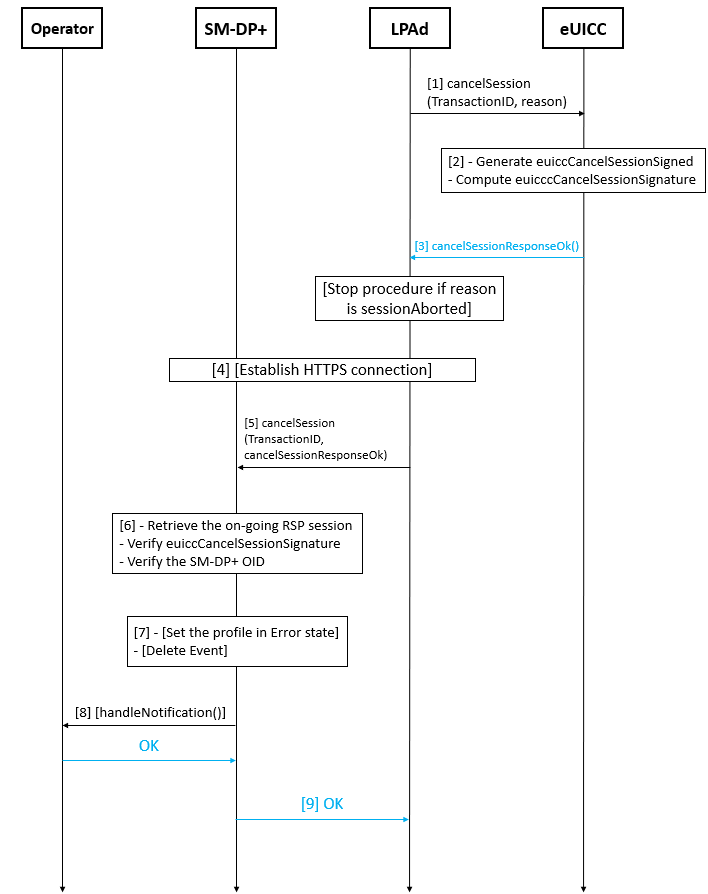
\includegraphics[width=\linewidth]{common-cancel-session.png}
\caption{Sequence diagram che descrive la Common Cancel Session Procedure.}
\label{fig:common-cancel-session}
\end{figure}

\subsubsection{Procedimento}
\begin{enumerate}
\item L'LPA invoca la funzione \textit{cancelSession} sull'eUICC, passandovi come parametri l'ID di transazione e la reason, ovvero il motivo per cui è stata avviata la Common Cancel Session Procedure.
\item L'eUICC esegue le seguenti operazioni:
\begin{itemize}[itemsep=0pt]
\item Generare la struttura dati euiccCancelSessionSigned che comprende l'ID di transazione e la reason, entrambi forniti dall'LPA.
\item Calcolare euiccCancelSessionSignature a partire da euiccCancelSessionSigned utilizzando la chiave privata SK.EUICC.SIG associata all'euiccCiPKIdToBeUsed ricevuto all'inizio della procedura di Common Mutual Authentication.
\end{itemize}
\item L'eUICC restituisce euiccCancelSessionSigned ed euiccCancelSessionSignature all'LPA. Se la reason è sessionAborted, allora l'LPA dovrà ignorare tale messaggio di risposta e interrompere la procedura.
\item Se la connessione HTTPS tra LPA e server SM-DP+ non è più attiva, allora l'LPA stabilisce una nuova connessione HTTPS col server come descritto nella procedura di Common Mutual Authentication.
\item L'LPA invoca la funzione \textit{cancelSession} anche sul server SM-DP+, passandovi come parametri l'ID della transazione, euiccCancelSessionSigned ed euiccCancelSessionSignature.
\item Il server SM-DP+ esegue le seguenti operazioni:
\begin{itemize}[itemsep=0pt]
\item Recuperare la sessione RSP corrente identificata dall'ID di transazione appena ricevuto.
\item Verificare euiccCancelSessionSignature.
\item Verificare che l'OID ricevuto sia uguale a quello contenuto in CERT.DPauth.SIG durante la procedura di Common Mutual Authentication.
\end{itemize}
Se anche solo uno di questi controlli non va a buon fine, o se l'ID di transazione ricevuto è ignoto, il server SM-DP+ deve restituire uno stato di errore e la procedura di Common Cancel Session deve essere interrotta. Inoltre, se la reason è postponed o timeout, allora il server deve mantenere l'ordinazione di download del profilo disponibile per ulteriori tentativi e passare allo step (9); in caso contrario, si procede con lo step successivo.
\item Il server SM-DP+ imposta il profilo allo stato Error. Inoltre, se un SM-DS è coinvolto nella sessione RSP, allora il server deve anche eliminare l'evento corrispondente dall'SM-DS.
\item Il server SM-DP+ può opzionalmente notificare l'operatore del fallimento del download del profilo mediante la funzione \textit{handleNotification}.
\item Il server SM-DP+ restituisce un acknowledgement all'LPA. A questo punto, la procedura termina.
\end{enumerate}

\section{Policy dei profili}\label{sec:profile-policy}
Come accennato nella sotto-sezione \ref{sec:down-install}, durante la procedura di download e installazione del profilo, è necessario anche verificare le policy del profilo per stabilire se quest'ultimo può essere installato all'interno dell'eUICC. Di conseguenza, può tornare utile illustrare nel dettaglio il meccanismo di gestione delle policy dei profili previsto in GSMA \cite{GSMA-docs-new}.\\
Le policy dei profili possono essere descritte dalle cosiddette \textbf{Profile Policy Rules} (PPR), che sono delle regole che descrivono cosa è possibile e cosa non è possibile fare con ciascun profilo. Attualmente possono essere definite due PPR in particolare:
\begin{itemize}
\item PPR1 - `Disabling of this Profile is not allowed'
\item PPR2 - `Deletion of this Profile is not allowed'
\end{itemize}

\subsection{Rules Authorisation Table}\label{sec:rat}
La Rules Authorisation Table (RAT) è una struttura dati che tiene traccia dell'insieme delle PPR accettabili per ciascun profilo \cite{GSMA-docs-new}. Da un punto di vista strutturale, la RAT mantiene una o più entry, ciascuna delle quali è relativa a una \textbf{Profile Policy Authorisation Rule} (PPAR). Una PPAR a sua volta è composta dalle seguenti informazioni (che costituiscono le colonne della tabella RAT):
\begin{itemize}
\item \textbf{Profile Policy Rule Identifier}: identifica una o più PPR a cui questa PPAR fa riferimento.
\item \textbf{Allowed Operators}: è una lista di operatori che possono utilizzare le PPR identificate dalla colonna Profile Policy Rule Identifier.
\item \textbf{End User Consent Required}: indica se, a seguito delle PPR identificate dalla colonna Profile Policy Rule Identifier, il profilo ha bisogno di un consenso esplicito dell'end user per essere installato.
\end{itemize}
In definitiva, la possibilità per un profilo di essere installato o meno dipende dalle eventuali PPR definite per quel profilo e dalle PPAR appartenenti alla RAT. In particolare:
\begin{itemize}
\item Se il profilo non contiene alcuna PPR, allora può essere installato senza problemi.
\item In caso contrario, è necessario verificare se nella RAT esistono delle PPAR che facciano riferimento sia alle PPR contenute nel profilo, sia all'operatore che ha rilasciato il profilo:
\begin{itemize}[itemsep=0pt]
\item Se tutte le PPR vengono coperte (da una o più PPAR) nell'ambito dell'operatore che ha rilasciato il profilo, allora si controlla la colonna End User Consent Required della RAT: i PPR per cui End User Consent Required = true hanno bisogno del consenso dell'end user affinché il relativo profilo possa essere installato nell'eUICC, e viceversa.
\item Se invece non tutte le PPR vengono coperte, non c'è la possibilità di installare il profilo nell'eUICC.
\end{itemize}
\end{itemize}
Si noti che il placeholder `*' per Allowed Operators indica ``tutti gli operatori". Se esistono più PPAR valide per una medesima PPR e un medesimo operatore, fa fede quella che compare per prima all'interno della RAT.\\
Il componente dell'eUICC che si occupa di verificare se un profilo contenente una o più PPR è autorizzato dalla RAT o meno è detto \textbf{Profile Policy Enabler} (PPE) \cite{GSMA-docs-new}.

\subsubsection{Primo esempio di RAT}
La tabella \ref{tab:rat1}, tratta da \cite{GSMA-docs-new}, raffigura un primo esempio di RAT.\\
\begin{table}[h!]
\begin{center}
\captionsetup{skip=4pt}
\caption{Primo esempio di RAT.}
\label{tab:rat1}
\begin{tabularx}{\textwidth}{|X|c|c|} % <-- Alignments: 2st column center and 3nd center, with vertical lines in between
\hline
\textbf{Profile Policy Rule Identifier} & \textbf{Allowed Operators} & \textbf{End User Consent Required}\\
\hline
PPR1 & OP-A & false\\
\hline
PPR2 & OP-B & false\\
\hline
PPR1, PPR2 & * & true\\
\hline
\end{tabularx}
\end{center}
\end{table}

\noindent La RAT rappresentata in \ref{tab:rat1} descrive la seguente situazione:
\begin{itemize}
\item L'operatore OP-A può usare PPR1 senza il consenso dell'end user e PPR2 col consenso dell'end user.
\item L'operatore OP-B può usare PPR1 col consenso dell'end user e PPR2 senza il consenso dell'end user.
\item Tutti gli altri operatori possono usare sia PPR1 che PPR2 col consenso dell'end user.
\end{itemize}

\subsubsection{Secondo esempio di RAT}
La tabella \ref{tab:rat2}, tratta da \cite{GSMA-docs-new}, raffigura un secondo esempio di RAT.\\
\begin{table}[h!]
\begin{center}
\captionsetup{skip=4pt}
\caption{Secondo esempio di RAT.}
\label{tab:rat2}
\begin{tabularx}{\textwidth}{|X|c|c|} % <-- Alignments: 2st column center and 3nd center, with vertical lines in between
\hline
\textbf{Profile Policy Rule Identifier} & \textbf{Allowed Operators} & \textbf{End User Consent Required}\\
\hline
PPR1, PPR2 & * & true\\
\hline
\end{tabularx}
\end{center}
\end{table}

\noindent Secondo la RAT rappresentata in \ref{tab:rat2}, tutti gli operatori possono usare PPR1 e PPR2 col consenso dell'end user.

\subsubsection{Terzo esempio di RAT}
Un terzo esempio classico è dato dalla tabella RAT vuota, secondo cui nessun operatore può usare alcuna PPR.

\chapter{Stato dell'arte}
\section{Uno studio condotto nel 2022}
Per quanto concerne la sicurezza dell'eSIM e del protocollo RSP, non sono ancora stati condotti numerosi studi e, al momento, risulta difficoltoso trovare degli articoli a riguardo in rete. Ciò è dovuto al fatto che questo mondo è del tutto nuovo e i telefoni che supportano le eSIM sono tuttora in fase di diffusione. Di conseguenza, in questo capitolo ci si limita a illustrare un particolare studio che, al momento, è di gran lunga il più importante a essere stato condotto nell'ambito dell'eSIM: si tratta di un'analisi portata a termine nel 2022 da quattro ricercatori dell'università Aalto in Finlandia (Abu Shohel Ahmed, Aleksi Peltonen, Mohit Sethi e Tuomas Aura) \cite{Sec-analysis}.\\
Il fine ultimo dello studio è quello di effettuare un'analisi di sicurezza del protocollo, a partire dalla procedura di Common Mutual Authentication fino al download e l'installazione del profilo, definendo 15 obiettivi di sicurezza, considerando due varianti del protocollo (default server approach e Activation Code approach) e lavorando su 11 scenari differenti, ciascuno dei quali viene analizzato sia con l'uso del tunnel TLS tra l'applicazione LPA e il server SM-DP+, sia senza l'uso del tunnel TLS. L'analisi è stata svolta con l'aiuto di ProVerif, un verificatore automatico di protocolli crittografici che lavora nel modello formale; in particolare, questo tool permette di dimostrare la validità di proprietà crittografiche come la confidenzialità, l'autenticazione, l'indistinguibilità tra più segreti e l'equivalenza di più processi client che differiscono esclusivamente nella sessione in cui comunicano col server \cite{ProVerif}.\\
La tabella \ref{tab:scenarios}, tratta da \cite{Sec-analysis}, elenca gli 11 scenari su cui si è lavorato. È chiaro che gli ultimi due sono applicabili soltanto nella variante del protocollo in cui è previsto l'uso dell'Activation Code (Activation Code approach).
\begin{table}[h!]
\begin{center}
\captionsetup{skip=4pt}
\caption{Gli 11 scenari considerati nello studio.}
\label{tab:scenarios}
\begin{tabularx}{\textwidth}{|c|c|X|} % <-- Alignments: 1st column center and 2nd center, with vertical lines in between
\hline
\textbf{N°} & \textbf{Scenario} & \textbf{Descrizione}\\
\hline
1 & Base-case & Tutti i partecipanti sono onesti e solo la rete tra l'LPA e il server SM-DP+ è untrusted.\\
\hline
2 & Server & L'attaccante possiede tutte le chiavi private del server SM-DP+.\\
\hline
3 & eUICC & L'attaccante possiede la chiave privata dell'eUICC del telefono della vittima.\\
\hline
4 & LPA & L'attaccante è l'utente che controlla l'LPA.\\
\hline
5 & 2nd server & Il server SM-DP+ target è onesto ma esiste un secondo server SM-DP+ compromesso.\\
\hline
6 & 2nd eUICC & L'attaccante possiede la chiave privata dell'eUICC del proprio telefono.\\
\hline
7 & 2nd MNO & L'operatore target è onesto ma esiste un secondo operatore compromesso.\\
\hline
8 & Order-user & L'attaccante impersona la vittima quando esegue l'ordine di un profilo.\\
\hline
9 & Order-eUICC & L'attaccante richiede un profilo per l'eUICC della vittima (senza impersonarla).\\
\hline
10 & AC leak & L'attaccante ottiene l'Activation Code associato a un profilo da scaricare.\\
\hline
11 & AC spoof & L'attaccante manipola l'LPA affinché utilizzi un Activation Code errato.\\
\hline
\end{tabularx}
\end{center}
\end{table}

\noindent D'altra parte, i 15 obiettivi di sicurezza, il cui conseguimento è stato testato negli scenari di cui sopra (con e senza tunnel TLS) sono schematizzati all'interno della tabella \ref{tab:security-goals} tratta da \cite{Sec-analysis}.
\begin{table}[h!]
\begin{center}
\captionsetup{skip=4pt}
\caption{I 15 obiettivi di sicurezza considerati nello studio.}
\label{tab:security-goals}
\begin{tabularx}{\textwidth}{|c|c|X|} % <-- Alignments: 1st column center and 2nd center, with vertical lines in between
\hline
\textbf{ID} & \textbf{Tipo} & \textbf{Descrizione}\\
\hline
A & Autenticazione & L'eUICC può completare l'autenticazione del server SM-DP+ solo dopo che entrambi gli end-point hanno avviato la procedura.\\
\hline
B & Autenticazione & Il server SM-DP+ può completare l'autenticazione dell'eUICC solo dopo aver avviato la procedura e dopo essere stato autenticato dall'eUICC.\\
\hline
B' & Autenticazione & Vi è una corrispondenza tra il completamento dell'autenticazione dell'eUICC, il fatto che l'end user sia l'effettivo proprietario dell'eUICC, la richiesta di un profilo all'operatore da parte dell'end user e la richiesta di ordinazione di quel profilo al server SM-DP+ da parte dell'operatore.\\
\hline
C & Autenticazione & L'eUICC può accettare il server SM-DP+ come entità da cui effettuare il download del profilo solo se la procedura di mutua autenticazione è stata completata con successo e se la GSMA ha autorizzato il server a rilasciare profili.\\
\hline
D & Autenticazione & Il server SM-DP+ può avviare il key agreement e la consegna del profilo solo se l'eUICC è stato autenticato e lo ha accettato come entità da cui effettuare il download del profilo.\\
\hline
E & Autenticazione & L'eUICC può accettare le chiavi di sessione solo se quest'ultimo ha avviato il key agreement.\\
\hline
F & Autenticazione & L'eUICC può scaricare il profilo dal server SM-DP+ solo se quest'ultimo ha avviato la consegna del profilo.\\
\hline
G & Autenticazione & Vi è una corrispondenza tra l'accettazione della notifica di download del profilo da parte del server SM-DP+, il fatto che l'end user sia l'effettivo proprietario dell'eUICC, la richiesta di un profilo all'operatore da parte dell'end user e la richiesta di ordinazione di quel profilo al server SM-DP+ da parte dell'operatore.\\
\hline
I & Autenticazione & L'eUICC può scaricare il profilo dal server SM-DP+ solo dopo che entrambi gli end-point hanno avviato la procedura di Common Mutual Authentication.\\
\hline
J & Autenticazione & Vi è una corrispondenza tra il download del profilo all'interno dell'eUICC, il fatto che l'end user sia l'effettivo proprietario dell'eUICC, la richiesta di un profilo all'operatore da parte dell'end user e la richiesta di ordinazione di quel profilo al server SM-DP+ da parte dell'operatore.\\
\hline
K & Autenticazione & Vi è una corrispondenza tra il rilascio del profilo da parte del server SM-DP+, il fatto che l'end user sia l'effettivo proprietario dell'eUICC, la richiesta di un profilo all'operatore da parte dell'end user e la richiesta di ordinazione di quel profilo al server SM-DP+ da parte dell'operatore.\\
\hline
W & Confidenzialità & L'attaccante non può accedere alle chiavi di sessione una volta che sono state accettate dal server SM-DP+.\\
\hline
X & Confidenzialità & L'attaccante non può accedere alle chiavi di sessione una volta che sono state accettate dall'eUICC.\\
\hline
Y & Confidenzialità & L'attaccante non può accedere al profilo decrittato una volta che è stato rilasciato dal server SM-DP+.\\
\hline
Z & Confidenzialità & L'attaccante non può accedere al profilo decrittato una volta che è stato scaricato nell'eUICC.\\
\hline
\end{tabularx}
\end{center}
\end{table}

\noindent I risultati dei test eseguiti dai quattro ricercatori dell'università Aalto sono illustrati in figura \ref{fig:results2022} tratta da \cite{Sec-analysis}.
\begin{figure}
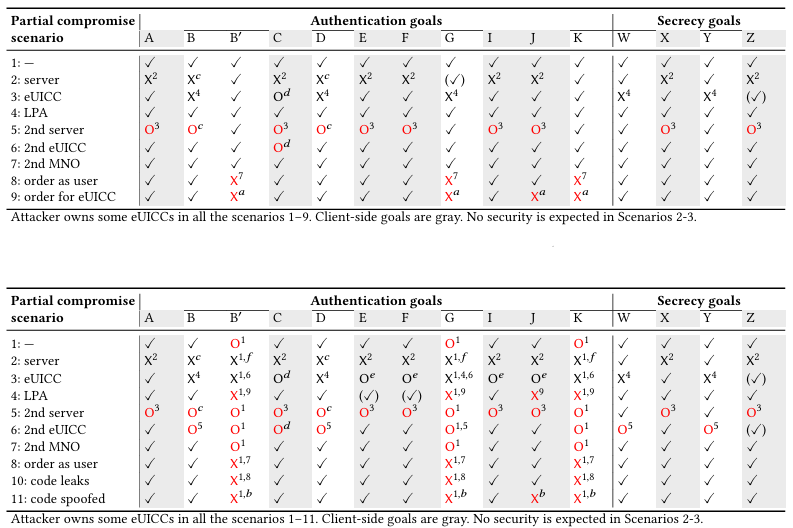
\includegraphics[width=\linewidth]{results2022.png}
\caption{Risultati dell'approccio default server (in alto) e Activation Code (in basso).}
\label{fig:results2022}
\end{figure}
La spunta indica che il controllo di sicurezza è passato, il cerchio indica che il controllo di sicurezza è passato solo nel caso in cui è presente il tunnel TLS, la spunta tra parentesi indica che il tool ProVerif ha terminato senza un risultato conclusivo, mentre la X indica che il controllo di sicurezza non è passato. Tutti i simboli colorati di rosso nelle due tabelle sono relativi a risultati inaspettati o comunque degni di nota: di fatto, i casi in cui l'attaccante possiede le chiavi private del server SM-DP+ o dell'eUICC sono gli unici in cui ci si aspettava con un elevato livello di confidenza che l'intero protocollo fosse compromesso.

\noindent Sulla base delle considerazioni riportate in \cite{Sec-analysis}, è possibile riassumere le vulnerabilità emerse nel seguente elenco.
\begin{enumerate}
\item Se si usa un server SM-DP+ S' compromesso a fianco del server SM-DP+ S coinvolto nella comunicazione RSP e non vi è un tunnel TLS tra l'LPA e il server S, allora l'attaccante può deviare la comunicazione verso il server S'. In tal modo, l'eUICC accetta anche i profili falsi generati dal server compromesso (S'). La vulnerabilità potrebbe essere dovuta al fatto che non compare alcun identificatore del server SM-DP+ (OID) all'interno dei messaggi che contengono i profili.
\item Se l'attaccante possiede l'eUICC U, viene compromesso un secondo eUICC U', non vi è un tunnel TLS tra l'LPA e il server SM-DP+ e si ricorre all'approccio Activation Code, allora l'attaccante può rubare l'Activation Code dalla vittima che possiede U, firmarlo con la chiave privata dell'eUICC compromesso (U') e inviare il messaggio così generato al server SM-DP+. In tal modo, il server risponde a U' (anziché a U) con il nuovo profilo. La vulnerabilità potrebbe essere dovuta al fatto che all'interno del server SM-DP+ non viene registrato l'identificatore dell'eUICC target (EID) nel momento in cui viene ordinato un nuovo profilo.
\item L'attaccante può scaricare un profilo in modo illegittimo sul proprio eUICC in uno dei seguenti due modi: il primo modo consiste nell'impersonare un utente legittimo deviando il download sul proprio eUICC; il secondo modo consiste nel ricostruire l'Activation Code a partire da leak di informazioni lasciati dall'utente vittima, dall'operatore oppure da una LPA modificata. La vulnerabilità potrebbe essere dovuta al fatto che, quando un utente richiede il download di un profilo, l'operatore non verifica in modo soddisfacente la sua identità: di fatto, non vi è alcun legame crittografico tra il profilo e l'end user che ne richiede il download, bensì è sufficiente esibire il codice di attivazione per dimostrare di essere il proprietario legittimo del profilo target.
\item L'attaccante può scaricare un profilo nell'eUICC vittima (U) con la propria sottoscrizione (e quindi in modo illegittimo) in uno dei seguenti due modi: il primo modo consiste nel conoscere l'identificatore (l'EID) dell'eUICC U e richiedere il download del profilo per conto di U; il secondo modo consiste nell'iniettare un Activation Code per conto di U, ad esempio tramite una LPA modificata.
\item Se si hanno due server SM-DP+ (S, S'), tra cui S' è compromesso, e non vi è un tunnel TLS tra l'LPA e il server S, allora l'attaccante può far sì che il server S impersoni il server S': così, durante la procedura di Common Mutual Authentication, S crederà di aver autenticato l'eUICC e l'eUICC crederà di aver autenticato S'. La vulnerabilità potrebbe essere dovuta al fatto che l'OID non viene incluso nei messaggi iniziali della Common Mutual Authentication.
\item Se si hanno due eUICC (U, U'), tra cui U' è compromesso, e non vi è un tunnel TLS tra l'LPA e il server SM-DP+, allora l'attaccante può intercettare l'autenticazione tra l'eUICC U e il server: così, alla fine della procedura di Common Mutual Authentication, U crederà di aver autenticato il server e il server crederà di aver autenticato U'. La vulnerabilità potrebbe essere dovuta al fatto che l'EID non viene incluso nei messaggi iniziali della Common Mutual Authentication.
\item Se non vi è un tunnel TLS tra l'LPA e il server SM-DP+ e si ricorre all'approccio Activation Code, allora, anche senza componenti compromessi, potrebbero rimanere dei leak di informazioni riguardanti l'Activation Code che un eventuale attaccante potrebbe sfruttare a proprio vantaggio.
\end{enumerate}
Tutti i punti sopra elencati, eccetto il terzo e il quarto, fanno riferimento a vulnerabilità che occorrerebbero nel caso in cui non si avesse un tunnel TLS tra l'applicazione LPA in utilizzo e il server SM-DP+ contattato dall'LPA. Tuttavia, si noti anche che le vulnerabilità illustrate possono essere sfruttate solo in situazioni molto particolari dove si hanno malfunzionamenti, componenti compromessi o requisiti imposti dalle specifiche di GSMA non rispettati (come l'assenza del tunnel TLS tra l'LPA e il server SM-DP+). Di conseguenza, rimane impossibile assumere che il protocollo RSP così definito non sia formalmente corretto.

\section{Altri studi in corso}
Tuttora vengono portati avanti degli studi sulla sicurezza dell'eSIM e si tengono delle conferenze a rigurardo. Un esempio è l'OffensiveCon, il cui talk sull'eSIM tenutosi nel maggio 2023 è disponibile su YouTube: https://www.youtube.com/watch?v=5oecn43xsDg.\\
Qui è stato discusso su come deployare un profilo custom definito manualmente, come installare applicazioni custom nell'eUICC e come sfruttare qualche vulnerabilià dell'eUICC (e.g. utilizzo di un toolkit per catturare informazioni, esecuzione di comandi sulla macchina vittima mediante una connessione custom). Comunque sia, di nuovo, non sono stati riscontrati problemi o vulnerabilità nella definizione formale del protocollo RSP.

\chapter{Implementazione dei simulatori}
\section{Obiettivo prefissato}
Lo scopo che è stato inizialmente definito per la fase operativa del presente lavoro è quello di costruire un simulatore sia per il client (composto da eUICC e LPA) sia per il server SM-DP+, in modo tale da:
\begin{enumerate}
\item creare un ecosistema simulato che funzioni secondo le specifiche di GSMA;
\item far comunicare ciascun simulatore rispettivamente con server SM-DP+ reali e con eUICC + LPA reali, con l'idea di verificare come questi rispondono se vengono sollecitati in modo diverso. In tal modo, con test opportuni, è possibile mettere alla prova le entità reali per stabilire se:
\begin{itemize}[itemsep=0pt]
\item è possibile ricavare qualche informazione in più o qualche vulnerabilità;
\item implementano ogni controllo e ogni messaggio secondo le specifiche di GSMA oppure accettano un qualche pacchetto non conforme (e.g. contenente una signature o un certificato non valido).
\end{itemize}
\end{enumerate}
Per aiutarsi con l'implementazione dei simulatori, è utile avere a disposizione una traccia che rappresenti un reale scambio di messaggi tra un'applicazione LPA e un server SM-DP+. Questa, assieme alla documentazione, può rappresentare il punto di riferimento a cui affidarsi per implementare nel modo più preciso e fedele possibile lo scambio di messaggi e i check effettuati dalle due controparti.

\section{Ottenimento delle catture su Wireshark}\label{sec:wireshark}
È stato effettuato il download di un nuovo profilo (i.e. piano tariffario) reale di Very Mobile su un apposito dispositivo mobile che supporta le eSIM. Lo scambio di messaggi che ha coinvolto l'LPA del dispositivo mobile e il server SM-DP+ di Very Mobile è stato salvato su una traccia PCAP con l'ausilio di un'apposita applicazione di cattura di pacchetti di rete. Com'è stato già detto, il traffico tra LPA e server è traffico HTTPS per cui, di base, la traccia che si ottiene mostra dei pacchetti protetti dal protocollo TLS, offuscando il contenuto dei messaggi previsti dalle specifiche di GSMA di cui si è parlato nel capitolo precedente.\\
Per questo motivo, durante la fase di cattura, è stato sfruttato un proxy relay che ha il compito di interporsi nella comunicazione tra l'LPA e il server SM-DP+. Ciò ha permesso di creare due sessioni TLS distinte: una tra il telefono e il proxy relay e l'altra tra il proxy relay e il server SM-DP+. Nel mezzo, il tool di proxy è stato in grado di decrittare il traffico ricevuto da un end-point per poi cifrarlo nuovamente verso l'altro end-point, salvando il traffico decrittato su una traccia (più precisamente tre tracce, ma ne è stata presa in considerazione una in particolare) che, quindi, contiene uno scambio di pacchetti dei quali è possibile accedere al payload, ovvero al contenuto dei messaggi dati dal protocollo RSP. Per far ciò, è stato necessario predisporre l'utilizzo del dispositivo mobile coi privilegi di root, per cui è buona norma non coinvolgere il proprio telefono personale nell'esperimento.\\
È dunque possibile osservare che sia l'applicazione LPA utilizzata sia il server SM-DP+ abbiano accettato di comunicare direttamente con un'entità (il proxy relay) il cui certificato TLS non è firmato da alcuna Certification Authority riconducibile a GSMA. Ciò è in linea con la trattazione già svolta sulle catene di certificati all'interno della sezione \ref{sec:certificates}.\\
Il file PCAP contenente la traccia così ottenuta è stato analizzato tramite Wireshark, che è un analizzatore di rete, e consente sia di mostrare tutti i dettagli relativi a uno scambio di pacchetti già salvato, sia di catturare a sua volta una traccia, almeno nel caso in cui il traffico di interesse coinvolga il sistema su cui il tool è installato.

\section{Analisi dei messaggi catturati}
Wireshark risulta fondamentale per individuare il formato esatto di ciascun pacchetto catturato all'interno della traccia. Innanzitutto è necessario stabilire quali sono i messaggi presenti all'interno del file PCAP per stabilire quale corrispondenza ci sia tra la comunicazione di riferimento tra l'LPA del dispositivo mobile e il server SM-DP+ di Very Mobile. In figura \ref{fig:all-msgs-pcap} è rappresentata la schermata di Wireshark che mostra la successione dei messaggi che sono stati scambiati durante la cattura.\\
\begin{figure}
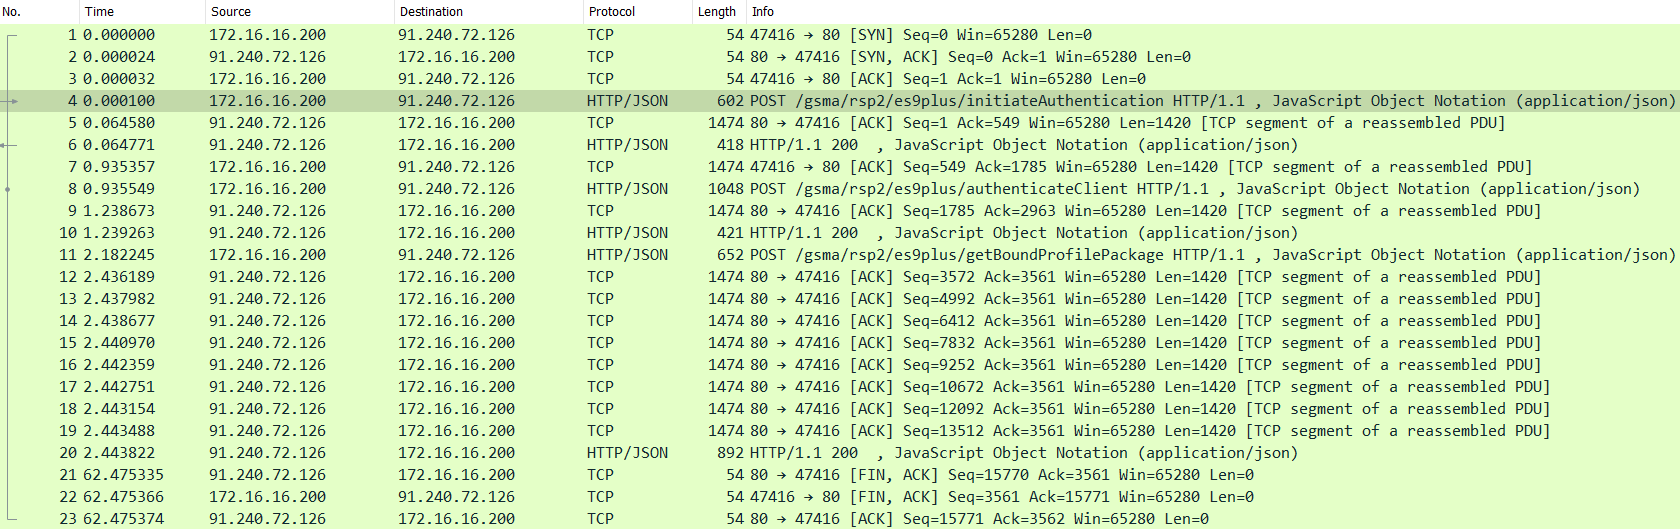
\includegraphics[width=\linewidth]{all-msgs-pcap.png}
\caption{Lista di pacchetti catturati.}
\label{fig:all-msgs-pcap}
\end{figure}
Com'è possibile vedere, in mezzo a dei normalissimi pacchetti TCP, spiccano alcuni pacchetti contrassegnati dal protocollo HTTP/JSON, che sono relativi proprio ai messaggi che compongono la comunicazione tra l'LPA e il server SM-DP+. In particolare, ve ne sono tre inviati al server da parte del client, mentre gli altri tre non sono altro che le rispettive risposte del server. I tre messaggi inviati dal client sono elencati qui di seguito:
\begin{enumerate}
\item \textbf{initiateAuthentication}, che corrisponde al primo messaggio inviato al server SM-DP+ da parte dell'LPA allo step (6) della procedura di Common Mutual Authentication (sezione \ref{sec:mutual-auth}).
\item \textbf{authenticateClient}, che corrisponde al secondo messaggio inviato al server SM-DP+ da parte dell'LPA allo step (15) della procedura di Common Mutual Authentication (sezione \ref{sec:mutual-auth}).
\item \textbf{getBoundProfilePackage}, che corrisponde al primo messaggio inviato al server SM-DP+ da parte dell'LPA allo step (5) della sotto-procedura di Download Confirmation (sezione \ref{sec:down-confirm}).
\end{enumerate}
Le risposte del server all'interno del file PCAP, nell'ordine, sono relative ai seguenti altri messaggi:
\begin{enumerate}
\item \textbf{initiateAuthenticationResponse}: corrisponde al messaggio inviato all'LPA da parte del server SM-DP+ allo step (9) della procedura di Common Mutual Authentication (sezione \ref{sec:mutual-auth}).
\item \textbf{authenticateClientResponse}, che corrisponde all'unico messaggio inviato all'LPA da parte del server SM-DP+ allo step (6) della procedura di download e installazione dei profili (sezione \ref{sec:down-install}).
\item \textbf{getBoundProfilePackageResponse}, che corrisponde al messaggio inviato all'LPA da parte del server SM-DP+ allo step (11) della sotto-procedura di Download Confirmation (sezione \ref{sec:down-confirm}).
\end{enumerate}
In realtà, le altre due tracce che sono state prese, oltre a questi sei pacchetti HTTP/JSON, riportano ulteriori messaggi contrassegnati dal medesimo protocollo, e sembrano corrispondere tutti a un \textbf{handleNotification} inviato al server SM-DP+ da parte dell'LPA in modo periodico: tale handleNotification è relativo all'ultimo messaggio ricevuto dal server allo step (14) della sotto-procedura di Download Confirmation (sezione \ref{sec:down-confirm}).\\
In definitiva, è possibile apprezzare un matching perfetto tra i pacchetti catturati nelle tracce PCAP e i messaggi previsti dalla documentazione di GSMA \cite{GSMA-docs-new} nel momento in cui si considerano in sequenza la procedura di Common Mutual Authentication e la procedura di download e installazione dei profili (inclusa la sotto-procedura di Download Confirmation).\\
Per comprendere appieno la struttura e il formato dei messaggi scambiati tra LPA e server SM-DP+, è certamente sufficiente effettuare un'analisi dettagliata del primo messaggio inviato dal client durante la procedura di Common Mutual Authentication (initiateAuthentication) e della relativa risposta del server (initiateAuthenticationResponse). Tuttavia, nella presente trattazione si intende effettuare un'analisi completa di tutti i pacchetti scambiati dalle controparti con lo scopo di acquisire più informazioni possibili sui messaggi ed, eventualmente, sul server SM-DP+ di Very Mobile e sul profilo installato all'interno dell'eUICC del dispositivo mobile.

\subsection{Analisi di initiateAuthentication}
Da Wireshark è possibile osservare il contenuto del messaggio initiateAuthentication all'interno della comunicazione reale tra LPA del dispositivo mobile e server SM-DP+ di Very Mobile. La figura \ref{fig:msg1-stream-pcap} ne mostra un estratto.\\
\begin{figure}
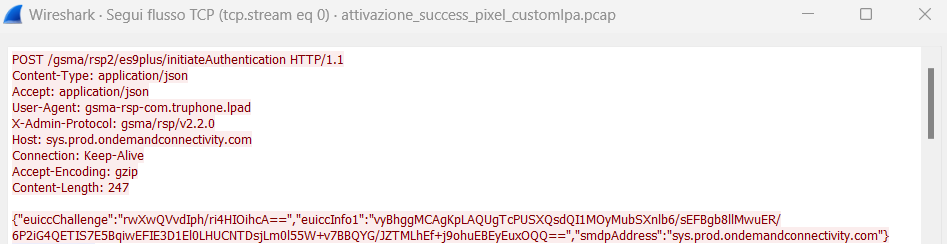
\includegraphics[width=\linewidth]{msg1-stream-pcap.png}
\caption{Messaggio di initiateAuthentication visualizzato su Wireshark.}
\label{fig:msg1-stream-pcap}
\end{figure}
L'header HTTP riporta alcune informazioni interessanti:
\begin{itemize}
\item il metodo HTTP utilizzato dall'LPA è POST;
\item la versione HTTP utilizzata è la 1.1;
\item il protocollo seguito per l'interazione tra LPA e server è la versione 2.2.0 di GSMA-RSP;
\item l'hostname del server SM-DP+ di Very Mobile è sys.prod.ondemandconnectivity.com;
\item l'LPA in questione accetta anche messaggi di risposta il cui payload è stato compresso tramite gzip.
\end{itemize}
Per quanto invece concerne il payload del messaggio, è possibile osservare che ha una struttura JSON con tre coppie chiave-valore. In particolare, i primi due campi, che sono euiccChallenge ed euiccInfo1, assumono dei valori rappresentati nella codifica \textbf{base64}, mentre il terzo e ultimo campo, ovvero smdpAddress, riporta in chiaro l'hostname del server SM-DP+ contattato.

\subsubsection{Codifica base64}
È un sistema di codifica che permette di convertire una sequenza di byte in una stringa in formato ASCII, dove i possibili caratteri diversi che compongono la stringa sono 64 \cite{RFC-4648}. Lo scopo della codifica è principalmente quello di rendere stampabile qualunque tipo di informazione.\\
L'idea alla base è molto semplice: si prende la sequenza di byte di partenza, la si suddivide in gruppi di 6 bit, e ciascun gruppo di 6 bit viene tradotto nel corrispondente carattere ASCII secondo la convenzione riportata nella figura \ref{fig:base64} tratta da \cite{RFC-4648}.\\
\begin{figure}
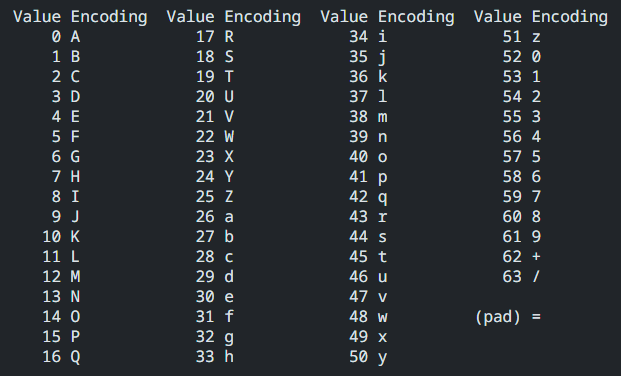
\includegraphics[width=\linewidth]{base64.png}
\caption{Tabella di conversione della codifica base64.}
\label{fig:base64}
\end{figure}
La tabella di conversione della codifica base64 riporta anche un sessantacinquesimo carattere ('='), che svolge la funzione di padding. Infatti, è possibile assumere che ogni sequenza di byte data in input all'algoritmo di codifica base64 abbia una lunghezza multipla di 8 bit, ma non è detto che abbia una lunghezza multipla anche di 6 bit; di fatto, avere una linghezza multipla di 6 bit significherebbe avere una lunghezza multipla di 24 bit. Si hanno dunque tre casistiche \cite{RFC-4648}:
\begin{enumerate}
\item La sequenza di byte di input ha una lunghezza multipla di 24 bit: in tal caso, non è necessario avere particolari accortezze e, in particolare, non è previsto alcun padding.
\item La sequenza di byte di input ha una lunghezza tale per cui alla fine avanzano 8 bit: in tal caso, vengono aggiunti 4 bit di padding pari a 0, vengono convertiti i 12 bit così ottenuti nei corrispettivi 2 caratteri ASCII e, in coda alla stringa di output, vengono aggiunti 2 caratteri di uguale ('==').
\item La sequenza di byte di input ha una lunghezza tale per cui alla fine avanzano 16 bit: in tal caso, vengono aggiunti 2 bit di padding pari a 0, vengono convertiti i 18 bit così ottenuti nei corrispettivi 3 caratteri ASCII e, in coda alla stringa di output, viene aggiunto un carattere di uguale ('=').
\end{enumerate}
Sulla base dell'algoritmo di conversione appena esposto, è possibile concludere che il campo euiccChallenge del messaggio è uguale al valore intero 232645733703218863597835671721642336624, mentre il campo euiccInfo1 risulta pari alla sequenza di byte mostrata in figura \ref{fig:asn1-euiccInfo1}.\\
\begin{figure}
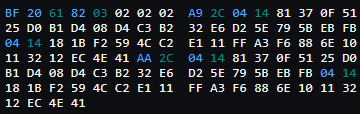
\includegraphics[width=\linewidth]{asn1-euiccInfo1.png}
\caption{Sequenza di byte che descrive euiccInfo1 in initiateAuthentication.}
\label{fig:asn1-euiccInfo1}
\end{figure}
Le specifiche di GSMA \cite{GSMA-docs-new} suggeriscono che i tipi di dato complessi come euiccInfo1 in RSP vengono rappresentati secondo lo standard \textbf{ASN.1} sfruttando la codifica \textbf{DER}.

\subsubsection{Codifica DER}
DER (Distinguished Encoding Rules) è una variante restrittiva di \textbf{BER} (Basic Encoding Rules) che, di fatto, elimina alcune flessibilità offerte da BER \cite{DER}.\\
BER a sua volta rappresenta un insieme di regole per la conversione di dati eterogenei in flussi di byte. Per la codifica, fa uso del formato \textbf{TLV} (Tag-Length-Value) e, per questa ragione, è particolarmente legato allo standard ASN.1 \cite{BER}. Di conseguenza, per comprendere al meglio il significato dei byte che compongono euiccInfo1, può risultare utile introdurre una panoramica generale sul funzionamento dello standard ASN.1.

\subsubsection{Standard ASN.1}
ASN.1 (Abstract Syntax Notation One) è uno standard di codifica che rappresenta le informazioni sfruttando il formato TLV, proprio come previsto dalle specifiche della codifica BER \cite{RFC-6025}\cite{ASN1}. Ciò significa che ciascuna unità di informazione è suddivisa in tre parti:
\begin{itemize}
\item \textbf{Tag}: detto anche \textbf{type}, è composto tipicamente da un byte e indica il tipo di dato che si sta rappresentando. Il tipo può essere primitivo (e.g. Boolean, Integer, UTF8String \cite{ASN1-types}), composto (e.g. Sequence, Set \cite{ASN1-types}), un metadato (e.g. Object Identifier \cite{ASN1-types}) oppure un tipo di dato custom; in quest'ultimo caso, spesso il tag è composto da due byte anziché da uno.
\item \textbf{Length}: è un campo che può essere composto da uno o più byte. Più precisamente, si hanno tre casi \cite{ASN1}:
\begin{itemize}[itemsep=0pt]
\item Campo length composto da un solo byte compreso tra 0x00 e 0x7F (i.e. tra 0 e 127): in tal caso l'unico byte rappresenta la lunghezza effettiva del campo value.
\item Campo length composto da più di un byte: in tal caso il primo byte deve essere compreso tra 0x81 e 0xFF (i.e. tra 129 e 255) ed è tale per cui il suo valore diminuito di 0x80 (i.e. 128) rappresenta la lunghezza della restante porzione del campo length. La restante porzione del campo length, invece, indica la lunghezza effettiva del campo value. Questa convenzione viene applicata tutte e sole le volte in cui il campo value è più lungo di 127 byte. Per fare un esempio, per indicare una lunghezza di value pari a 257 byte, il campo length deve essere uguale a 0x820101: il primo byte (0x82) indica che, oltre a lui stesso, si hanno ulteriori due byte (i.e. 0x82-0x80) a comporre il campo length; gli ultimi due byte (0x0101), invece, stanno a indicare esattamente la lunghezza del campo value, che è proprio pari a 257.
\item Campo length il cui primo byte è pari a 0x80: in tal caso, si ha una length ``indefinita", per cui è verosimilmente sintomo di una formattazione errata.
\end{itemize}
\item \textbf{Value}: è il campo che contiene il payload vero e proprio dell'informazione che si sta rappresentando. Nel caso particolare in cui il relativo tipo di dato è composto, tale campo è costituito a sua volta da altri elementi TLV, creando così un'annidazione che può essere ricorsiva a piacere \cite{ASN1}.
\end{itemize}
Comunque sia, conoscere lo standard ASN.1 non è sufficiente per interpretare in modo agevole le sequenze di byte come quella in figura \ref{fig:asn1-euiccInfo1} che è relativa a euiccInfo1. Infatti, a primo impatto si intuisce solo che euiccInfo1 è composto a sua volta da tre elementi in formato TLV (che iniziano rispettivamente coi byte 0x8203, 0xA92C, 0xAA2C), ma il loro significato non è chiaro. Di seguito è riportata la definizione precisa della struttura dati euiccInfo1 tratta da \cite{RSP-definitions}.\\

\textit{EUICCInfo1 ::= [32] SEQUENCE \{ \textcolor{gray}{{-}{-} Tag `BF20'}}

\hspace{0.75cm} \textit{svn [2] VersionType, \textcolor{gray}{{-}{-} GSMA SGP.22 version supported (SVN)}}

\hspace{0.75cm} \textit{euiccCiPKIdListForVerification [9] SEQUENCE OF SubjectKeyIdentifier,}

\hspace{0.75cm} \textit{euiccCiPKIdListForSigning [10] SEQUENCE OF SubjectKeyIdentifier}

\textit{\}\\}

\noindent Come si può evincere, euiccInfo1 è una struttura dati composta da alcune informazioni che caratterizzano l'eUICC del dispositivo mobile coinvolto nella comunicazione. Tali informazioni sono schematizzate di seguito.
\begin{itemize}
\item lo Specification Version Number (SVN), che sarebbe la versione di GSMA SGP.22 supportata dall'eUICC;
\item una lista (Sequence) di identificatori delle chiavi pubbliche del CI che possono essere utilizzate dall'eUICC per autenticare il server;
\item una lista (Sequence) di identificatori delle chiavi pubbliche del CI che possono essere utilizzate dall'eUICC per firmare i propri dati.
\end{itemize}
Si noti che questa definizione di euiccInfo1 combacia perfettamente con le specifiche di GSMA \cite{GSMA-docs-new} relative alla procedura di Common Mutual Authentication \ref{sec:mutual-auth}.\\
Per determinare nel modo più agevole possibile i valori assunti dai tre campi di euiccInfo1 sopra elencati, si può far riferimento al sito https://lapo.it/asn1js/ (\textit{ASN.1 JavaScript decoder}) il quale, data una stringa base64, restituisce in chiaro le informazioni codificate con lo standard ASN.1. In figura \ref{fig:decode-euiccInfo1} è riportato l'output del sito \textit{ASN.1 JavaScript decoder} nel momento in cui gli viene dato in pasto la stringa base64 associata a euiccInfo1 in figura \ref{fig:msg1-stream-pcap}.
\begin{figure}
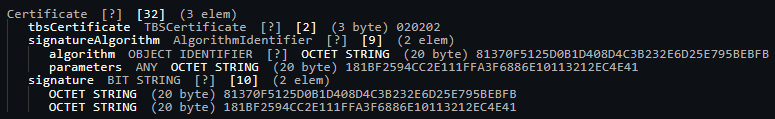
\includegraphics[width=\linewidth]{decode-euiccInfo1.png}
\caption{Decodifica del campo euiccInfo1 di initiateAuthentication.}
\label{fig:decode-euiccInfo1}
\end{figure}
In definitiva:
\begin{itemize}
\item SVN è pari alla sequenza di byte 0x020202, che verosimilmente indica la versione 2.2.2;
\item euiccCiPKIdListForVerification ed euiccCiPKIdListForSigning sono due liste identiche ciascuna delle quali contiene due identificatori di chiavi pubbliche del CI.
\end{itemize}

\subsection{Analisi di initiateAuthenticationResponse}
La figura \ref{fig:msg2-stream-pcap} mostra l'intero contenuto del primo messaggio di risposta del server SM-DP+.\\
\begin{figure}
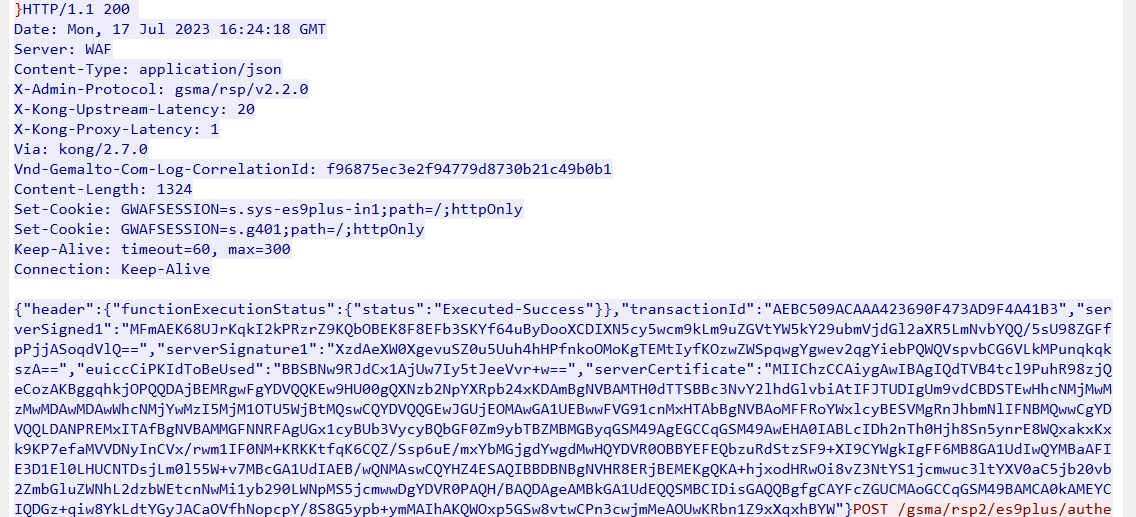
\includegraphics[width=\linewidth]{msg2-stream-pcap.png}
\caption{Messaggio di initiateAuthenticationResponse visualizzato su Wireshark.}
\label{fig:msg2-stream-pcap}
\end{figure}
Nell'header HTTP si ritrovano alcuni punti in comune col messaggio inviato dall'LPA: ad esempio, anche qui la versione HTTP utilizzata è la 1.1 e il protocollo usato per l'interazione tra LPA e server è la versione 2.2.0 di GSMA-RSP.\\

\noindent Il payload del messaggio ha una struttura JSON del tutto analoga a quella di initiateAuthentication. In particolare, si hanno i seguenti campi:
\begin{itemize}
\item \textbf{header}: è un campo in chiaro che indica l'esito del processamento del messaggio dell'LPA al livello del protocollo RSP. La presenza di \textit{\{``status":``Executed-Success"\}} indica che tutti i check sulle informazioni ricevute dal client sono andati a buon fine e la comunicazione può proseguire secondo le specifiche di GSMA;
\item \textbf{transactionId}: è un campo in chiaro che indica l'ID della transazione;
\item \textbf{serverSigned1}: è un campo codificato in base64;
\item \textbf{serverSignature1}: è un altro campo codificato in base64 che, come enunciato nella sezione \ref{sec:mutual-auth}, rappresenta la signature di serverSigned1;
\item \textbf{euiccCiPKIdToBeUsed}: è il terzo campo codificato in base64;
\item \textbf{serverCertificate}: è l'ultimo campo codificato in base64. La sua lunghezza è giustificata dal fatto che, con riferimento alla sezione \ref{sec:mutual-auth}, rappresenta il certificato CERT.DPauth.SIG, che è verosimilmente una struttura dati molto complessa.
\end{itemize}
Per comprendere appieno le informazioni celate nei campi di initiateAuthenticationResponse codificati in base64, si fa nuovamente riferimento a \cite{RSP-definitions} e al sito \textit{ASN.1 JavaScript decoder}.\\

\noindent La struttura dati serverSigned1 è molto semplice: dalla sua definizione riportata di seguito e dalla figura \ref{fig:decode-serverSigned1} \cite{RSP-definitions}, si capisce che è composta dall'ID di transazione, dalla challenge (euiccChallenge) che il server aveva ricevuto in initiateAuthentication, dall'hostname del server e da una nuova challenge generata dal server (serverChallenge).\\
\begin{figure}
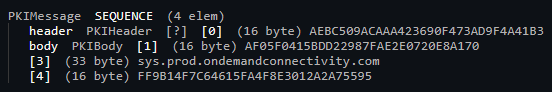
\includegraphics[width=\linewidth]{decode-serverSigned1.png}
\caption{Decodifica del campo serverSigned1 di initiateAuthenticationResponse.}
\label{fig:decode-serverSigned1}
\end{figure}

\textit{ServerSigned1 ::= [32] SEQUENCE \{}

\hspace{0.75cm} \textit{transactionId [0] TransactionId, \textcolor{gray}{{-}{-} The Transaction ID generated by the RSP Server}}

\hspace{0.75cm} \textit{euiccChallenge [1] Octet16, \textcolor{gray}{{-}{-} The eUICC Challenge}}

\hspace{0.75cm} \textit{serverAddress [3] UTF8String, \textcolor{gray}{{-}{-} The RSP Server address}}

\hspace{0.75cm} \textit{serverChallenge [4] Octet16, \textcolor{gray}{{-}{-} The RSP Server Challenge}}

\textit{\}\\}

\noindent Il campo euiccCiPKIdToBeUsed cela anch'esso una struttura TLV dello standard ASN.1, com'è possibile vedere dalle figure \ref{fig:asn1-euiccCiPKIdToBeUsed}, \ref{fig:decode-euiccCiPKIdToBeUsed}. Inoltre, il relativo campo value assume un valore che è comparso sia in euiccCiPKIdListForVerification, sia in euiccCiPKIdListForSigning, il che vuol dire che il server SM-DP+ accetta l'utilizzo di una delle due chiavi pubbliche di CA (i.e. una delle due certificate chain) proposte dal client nel messaggio initiateAuthentication.\\

\noindent Per quanto invece riguarda il campo serverCertificate di initiateAuthenticationResponse, il sito \textit{ASN.1 JavaScript decoder} aiuta a comprendere molti dettagli sul certificato CERT.DPauth.SIG e sulla relativa certificate chain utilizzata. Le figure \ref{fig:decode-serverCertificate1}, \ref{fig:decode-serverCertificate2} mostrano la decodifica di tale certificato. Inizialmente vi sono gli attributi fondamentali, come:
\begin{itemize}
\item \textbf{signature AlgorithmIdentifier}: indica con quale algoritmo vengono calcolate le signature mediante la chiave privata associata al certificato ed è pari a \textit{ecdsaWithSHA256} (ANSI X.962 ECDSA algorithm with SHA256);
\item \textbf{issuer Name}: è un campo relativo alla CA che ha rilasciato il presente certificato ed è a sua volta articolato in due sotto-campi, che sono l'organizationName (pari a ``GSM Association") e il commonName (pari a ``GSM Association - RSP2 Root CI1");
\item \textbf{validity Validity}: dichiara che il certificato è valido dal 30 marzo 2023 al 29 marzo 2026, il che corrisponde a tre anni;
\item \textbf{subject Name}: è un campo che fornisce dettagli informativi sul presente certificato ed è a sua volta composto in diversi sotto-campi, tra cui countryName (pari a ``FR", i.e. Francia), localityName (pari a ``Tours"), organizationName (pari a ``Thales DIS France SA"), organizationalUnitName (pari a ``ODC") e commonName (pari a ``SMDP Plus Tours Platform").
\item \textbf{subjectPublicKeyInfo SubjectPublicKeyInfo}: fornisce maggiori informazioni sulle chiavi associate al certificato, tra cui la curva ellittica utilizzata per generare le signature, che è identificata con \textit{prime256v1}.
\end{itemize}
Più in basso nel certificato si trovano le cosiddette estensioni, ovvero informazioni aggiuntive opzionali che possono essere inserite a piacimento all'interno del certificato. Tra queste è possibile individuare:
\begin{itemize}
\item \textbf{subjectKeyIdentifier}: è l'identificatore della chiave pubblica associata al presente certificato;
\item \textbf{authorityKeyIdentifier}: è l'identificatore della chiave pubblica dell'issuer del certificato e, per coerenza, deve corrispondere o contenere il valore associato al campo euiccCiPKIdToBeUsed del messaggio initiateAuthenticationResponse;
\item \textbf{keyUsage}: rappresenta i possibili utilizzi delle chiavi associate al certificato;
\item \textbf{subjectAltName}: rappresenta il nome alternativo dell'entità che possiede il certificato;
\item altre informazioni che non verranno esaminate a fondo in questa trattazione, come certificatePolicies e cRLDistributionPoints.
\end{itemize}
Infine, in fondo al certificato, si hanno ulteriori informazioni riguardanti la signature e l'algoritmo di signature.
\begin{figure}
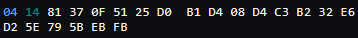
\includegraphics[width=\linewidth]{asn1-euiccCiPKIdToBeUsed.png}
\caption{Sequenza di byte che descrive euiccCiPKIdToBeUsed in initiateAuthenticationResp.}
\label{fig:asn1-euiccCiPKIdToBeUsed}
\end{figure}
\begin{figure}

\includegraphics[width=\linewidth]{decode-euiccCiPKIdToBeUsed.png}
\caption{Decodifica del campo euiccCiPKIdToBeUsed di initiateAuthenticationResponse.}
\label{fig:decode-euiccCiPKIdToBeUsed}
\end{figure}
\begin{figure}
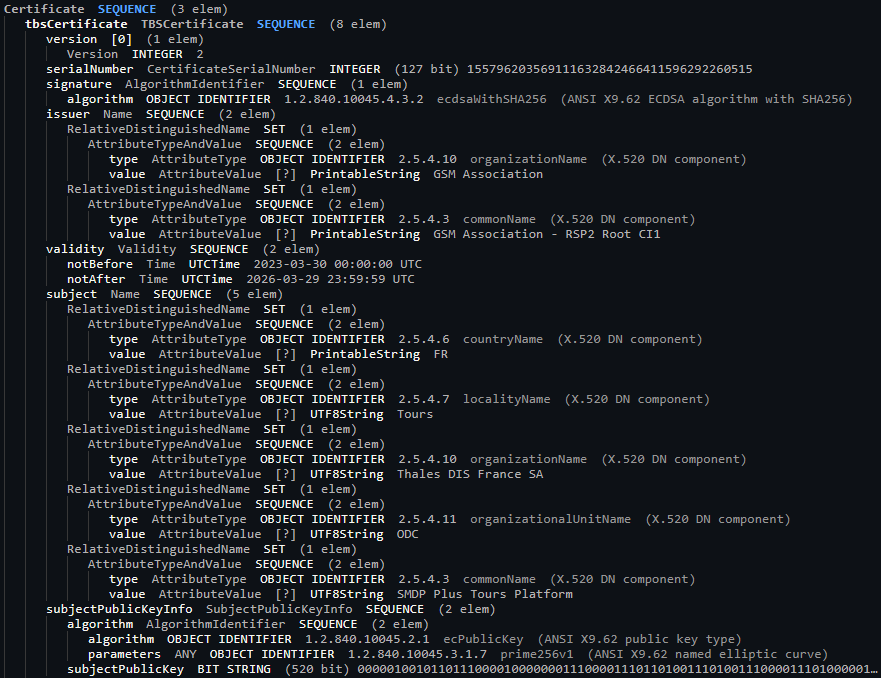
\includegraphics[width=\linewidth]{decode-serverCertificate1.png}
\caption{Decodifica del campo serverCertificate di initiateAuthenticationResponse (parte 1/2).}
\label{fig:decode-serverCertificate1}
\end{figure}
\begin{figure}
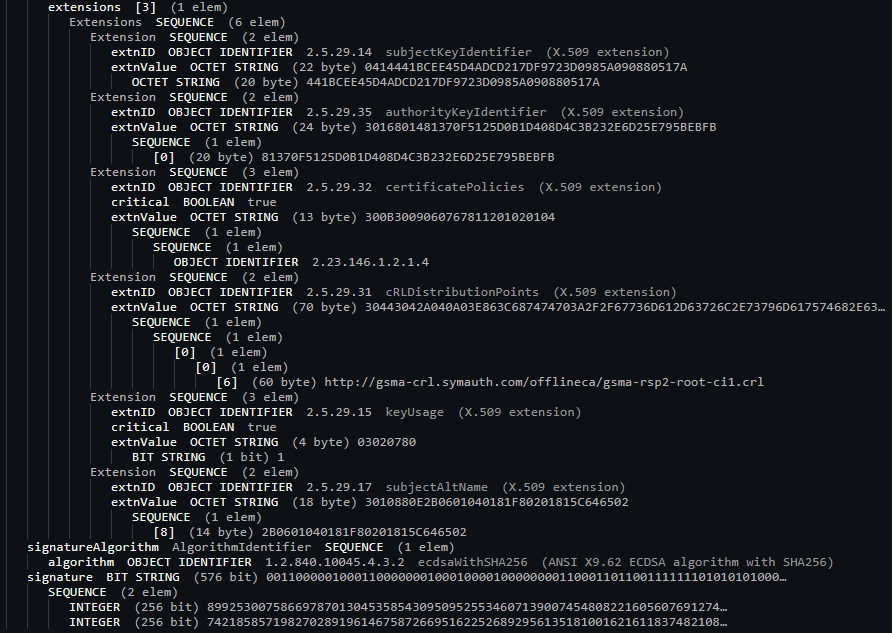
\includegraphics[width=\linewidth]{decode-serverCertificate2.png}
\caption{Decodifica del campo serverCertificate di initiateAuthenticationResponse (parte 2/2).}
\label{fig:decode-serverCertificate2}
\end{figure}

\subsection{Analisi di authenticateClient}
La figura \ref{fig:msg3-stream-pcap} mostra il contenuto del secondo messaggio inviato dal client (authenticateClient).\\
\begin{figure}
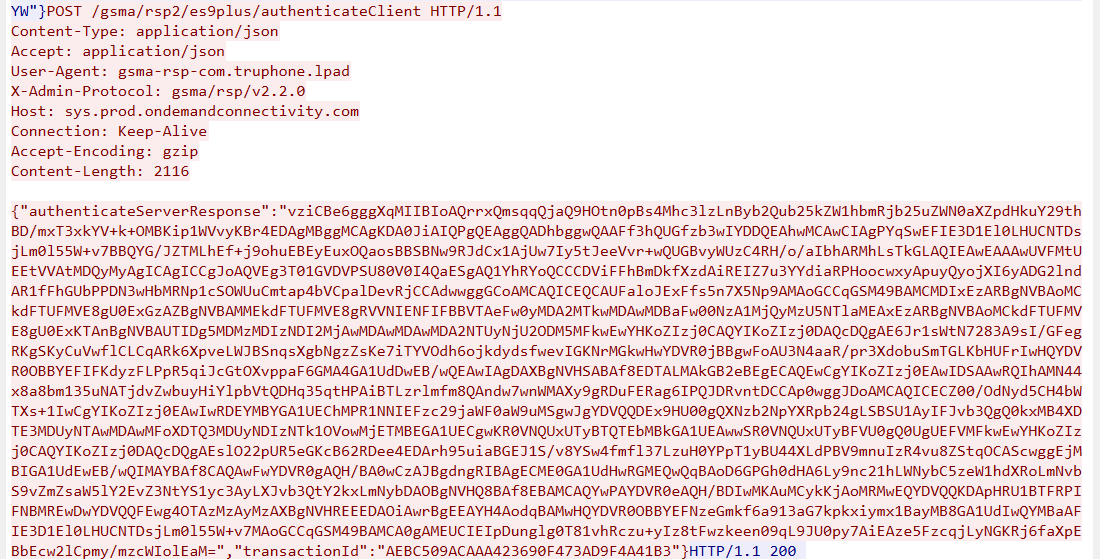
\includegraphics[width=\linewidth]{msg3-stream-pcap.png}
\caption{Messaggio di authenticateClient visualizzato su Wireshark.}
\label{fig:msg3-stream-pcap}
\end{figure}
Il JSON del payload è composto da due campi:
\begin{itemize}
\item \textbf{authenticateServerResponse}: è una struttura dati che verrà approfondita tra poco;
\item \textbf{transactionId}: corrisponde all'ID di transazione appena ricevuto nel messaggio initiateAuthenticationResponse.
\end{itemize}
Per quanto riguarda authenticateServerResponse, è una struttura composta da più elementi ASN.1 di tipo Sequence anche annidati tra loro, ed è descritta nella definizione riportata nelle pagine successive\cite{RSP-definitions}.\\

\textit{AuthenticateServerResponse ::= [56] CHOICE \{ \textcolor{gray}{{-}{-} Tag `BF38'}}

\hspace{0.75cm} \textit{authenticateResponseOk AuthenticateResponseOk,}

\hspace{0.75cm} \textit{authenticateResponseError AuthenticateResponseError}

\textit{\}\\}

\textit{AuthenticateResponseOk ::= SEQUENCE \{}

\hspace{0.75cm} \textit{euiccSigned1 EuiccSigned1, \textcolor{gray}{{-}{-} Signed information}}

\hspace{0.75cm} \textit{euiccSignature1 [APPLICAION 55] OCTET STRING, \textcolor{gray}{{-}{-} EUICC\_Sign1, tag `5F37'}}

\hspace{0.75cm} \textit{euiccCertificate Certificate, \textcolor{gray}{{-}{-} CERT.EUICC.ECDSA signed by the EUM}}

\hspace{0.75cm} \textit{eumCertificate Certificate \textcolor{gray}{{-}{-} CERT.EUM.ECDSA signed by the CI}}

\textit{\}\\}

\textit{EuiccSigned1 ::= SEQUENCE \{}

\hspace{0.75cm} \textit{transactionId [0] TransactionId,}

\hspace{0.75cm} \textit{serverAddress [3] UTF8String,}

\hspace{0.75cm} \textit{serverChallenge [4] Octet16, \textcolor{gray}{{-}{-} The RSP Server Challenge}}

\hspace{0.75cm} \textit{euiccInfo2 [34] EUICCInfo2,}

\hspace{0.75cm} \textit{ctxParams1 CtxParams1}

\textit{\}\\}

\textit{EUICCInfo2 ::= [34] SEQUENCE \{ \textcolor{gray}{{-}{-} Tag `BF22'}}

\hspace{0.75cm} \textit{profileVersion [1] VersionType, \textcolor{gray}{{-}{-} SIMAlliance Profile package version supported}}

\hspace{0.75cm} \textit{svn [2] VersionType, \textcolor{gray}{{-}{-} GSMA SGP.22 version supported (SVN)}}

\hspace{0.75cm} \textit{euiccFirmwareVer [3] VersionType, \textcolor{gray}{{-}{-} eUICC Firmware version}}

\hspace{0.75cm} \textit{extCardResource [4] OCTET STRING, \textcolor{gray}{{-}{-} Extended Card Resource Information}}

\hspace{0.75cm} \textit{uiccCapability [5] UICCCapability,}

\hspace{0.75cm} \textit{ts102241Version [6] VersionType OPTIONAL,}

\hspace{0.75cm} \textit{globalplatformVersion [7] VersionType OPTIONAL,}

\hspace{0.75cm} \textit{rspCapability [8] RspCapability,}

\hspace{0.75cm} \textit{euiccCiPKIdListForVerification [9] SEQUENCE OF SubjectKeyIdentifier,}

\hspace{0.75cm} \textit{euiccCiPKIdListForSigning [10] SEQUENCE OF SubjectKeyIdentifier,}

\hspace{0.75cm} \textit{euiccCategory [11] INTEGER \{}

\hspace{1.5cm} \textit{other(0),}

\hspace{1.5cm} \textit{basicEuicc(1),}

\hspace{1.5cm} \textit{mediumEuicc(2),}

\hspace{1.5cm} \textit{contactlessEuicc(3)}

\hspace{0.75cm} \textit{\} OPTIONAL,}

\hspace{0.75cm} \textit{forbiddenProfilePolicyRules [25] PprIds OPTIONAL, \textcolor{gray}{{-}{-} Tag `99'}}

\hspace{0.75cm} \textit{ppVersion VersionType, \textcolor{gray}{{-}{-} Protection Profile version}}

\hspace{0.75cm} \textit{sasAcreditationNumber UTF8String (SIZE(0..64)),}

\hspace{0.75cm} \textit{certificationDataObject [12] CertificationDataObject OPTIONAL}

\textit{\}\\}

\textit{CtxParams1 ::= CHOICE \{}

\hspace{0.75cm} \textit{ctxParamsForCommonAuthentication CtxParamsForCommonAuthentication}

\textit{\}\\}

\textit{CtxParamsForCommonAuthentication ::= SEQUENCE \{}

\hspace{0.75cm} \textit{matchingId UTF8String OPTIONAL,}

\hspace{0.75cm} \textit{deviceInfo DeviceInfo \textcolor{gray}{{-}{-} The Device information}}

\textit{\}\\}

\noindent Com'è possibile osservare, authenticateServerResponse si articola in due casi: authenticateResponseOk nel caso in cui l'autenticazione del server SM-DP+ sia andata a buon fine, e authenticateResponseError in caso contrario. La struttura authenticateResponseError è composta semplicemente dall'ID di transazione e da un codice di errore \cite{RSP-definitions}, mentre la struttura authenticateResponseOk è molto più articolata.\\
Anzitutto, authenticateResponseOk è composto da quattro campi: euiccSigned1 che è a sua volta un'altra struttura dati complessa, euiccSignature1 che, come ormai suggerisce il nome, rappresenta la firma digitale di euiccSigned1, il certificato dell'eUICC (CERT.EUICC.SIG) e il certificato dell'EUM (CERT.EUM.SIG). La struttura euiccSigned1 si articola in:
\begin{itemize}
\item \textbf{transactionId}: è l'ID della transazione;
\item \textbf{serverAddress}: è l'hostname del server SM-DP+;
\item \textbf{serverChallenge}: è la challenge generata precedentemente dal server e comunicata al client mediante il messaggio initiateAuthenticationResponse;
\item \textbf{euiccInfo2}: è un'ulteriore struttura dati che comprende tutte le informazioni sull'eUICC che si sta per autenticare e su cui avverrà l'installazione del nuovo profilo. È un sovrainsieme del campo euiccInfo1 di initiateAuthentication;
\item \textbf{ctxParams1}: come suggerito dal nome, rappresenta i parametri di contesto e, in particolar modo, le informazioni del dispositivo e il Matching ID. Quest'ultimo è tipicamente un token associato all'Activation Code (codice di attivazione) \cite{RSP-definitions}, il quale viene negoziato da server SM-DP+ e operatore durante la fase di \textit{profile ordering} e viene rilasciato dall'operatore mediante un'apposita email durante la fase di \textit{download initialization} (sezione \ref{sec:step-RSP}). Un estratto dell'email di Very Mobile relativa al profilo che si sta per installare sull'eUICC del dispositivo mobile di riferimento è riportato in figura \ref{fig:email}.
\end{itemize}
\begin{figure}
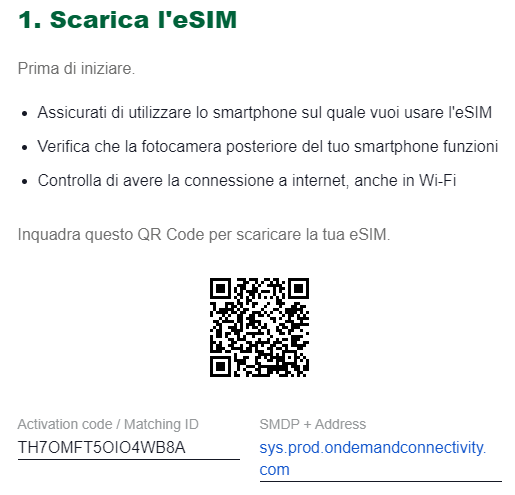
\includegraphics[width=\linewidth]{email.png}
\caption{Estratto dell'email di Very Mobile.}
\label{fig:email}
\end{figure}
La figura \ref{fig:decode-euiccSigned1} mostra come il sito \textit{ASN.1 JavaScript decoder} decodifica il campo euiccSigned1 a partire dalla stringa base64 relativa all'ASN.1 del campo authenticateServerResponse del messaggio authenticateClient. A partire dalla sestultima riga dell'immagine si ha la traduzione della struttura ctxParams1: qui si nota la corrispondenza tra il sotto-campo matchingId e l'Activation Code presente nell'email di cui sopra.
\begin{figure}
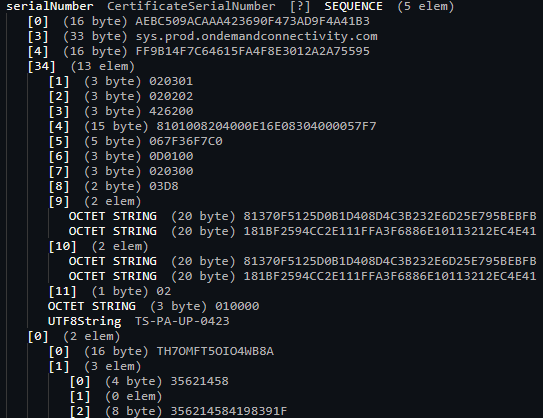
\includegraphics[width=\linewidth]{decode-euiccSigned1.png}
\caption{Decodifica del campo euiccSigned1 di authenticateServerResponse.}
\label{fig:decode-euiccSigned1}
\end{figure}

\subsection{Analisi di authenticateClientResponse}
La figura \ref{fig:msg4-stream-pcap} mostra il contenuto della risposta del server al secondo messaggio inviato dal client (authenticateClientResponse).\\
\begin{figure}
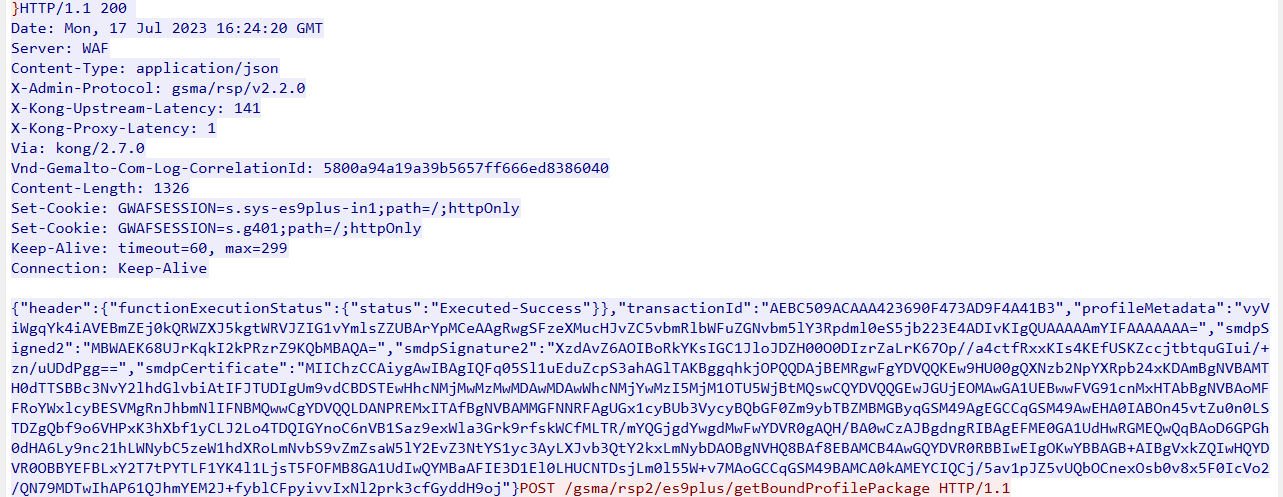
\includegraphics[width=\linewidth]{msg4-stream-pcap.png}
\caption{Messaggio di authenticateClientResponse visualizzato su Wireshark.}
\label{fig:msg4-stream-pcap}
\end{figure}
Il JSON del payload è composto dai campi elencati qui di seguito:
\begin{itemize}
\item \textbf{header}: contiene di nuovo \textit{\{``status":``Executed-Success"\}}, il che vuol dire che anche in questa fase tutti i check effettuati dal server SM-DP+ hanno avuto successo;
\item \textbf{transactionId}: è l'ID di transazione e assume sempre il medesimo valore;
\item \textbf{profileMetadata}: è un campo codificato in base64 che, come suggerisce il nome, dovrebbe comprendere i metadati del profilo di cui si sta per effettuare il download;
\item \textbf{smdpSigned2}: è un campo codificato in base64 che, come suggerisce il nome, dovrebbe essere strutturalmente simile a serverSigned1 e a euiccSigned1;
\item \textbf{smdpSignature2}: è un campo codificato in base64 relativo alla signature di smdpSigned2;
\item \textbf{smdpCertificate}: è un ultimo campo codificato in base64 che, con riferimento alla sezione \ref{sec:down-install}, rappresenta il certificato CERT.DPpb.SIG, che è potenzialmente diverso dal certificato CERT.DPauth.SIG inviato all'LPA precedentemente e viene utilizzato per firmare il profilo che si sta per scaricare.
\end{itemize}
I campi che possono essere approfonditi con l'aiuto di \cite{RSP-definitions} e del sito \textit{ASN.1 JavaScript decoder} sono profileMetadata (la cui sequenza di byte in ASN.1 è mostrata in figura \ref{fig:asn1-profileMetadata}) e smdpSigned2.\\

\noindent La struttura dati profileMetadata, come riportato di seguito, comprende informazioni sul profilo target come l'ICCID (che, come spiegato nella sezione \ref{sec:device-change}, è l'identificativo del profilo), il nome dell'operatore, il nome del profilo, la classe del profilo ed eventuali Profile Policy Rules.\\

\textit{StoreMetadataRequest ::= [37] SEQUENCE \{ \textcolor{gray}{{-}{-} Tag `BF25'}}

\hspace{0.75cm} \textit{iccid Iccid,}

\hspace{0.75cm} \textit{serviceProviderName [17] UTF8String (SIZE(0..32)), \textcolor{gray}{{-}{-} Tag `91'}}

\hspace{0.75cm} \textit{profileName [18] UTF8String (SIZE(0..64)), \textcolor{gray}{{-}{-} Tag `92'}}

\hspace{0.75cm} \textit{iconType [19] IconType OPTIONAL, \textcolor{gray}{{-}{-} Tag `93' (JPG or PNG)}}

\hspace{0.75cm} \textit{icon [20] OCTET STRING (SIZE(0..1024)), \textcolor{gray}{{-}{-} Tag `94' (Data of the icon)}}

\hspace{0.75cm} \textit{profileClass [21] ProfileClass DEFAULT operational, \textcolor{gray}{{-}{-} Tag `95'}}

\hspace{0.75cm} \textit{notifConfig [22] SEQUENCE OF NotificationConfigurationInformation OPTIONAL,}

\hspace{0.75cm} \textit{profileOwner [23] OperatorId OPTIONAL, \textcolor{gray}{{-}{-} Tag `B7'}}

\hspace{0.75cm} \textit{profilePolicyRules [25] PprIds OPTIONAL \textcolor{gray}{{-}{-} Tag `99'}}

\textit{\}\\}

\begin{figure}
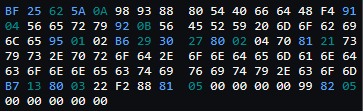
\includegraphics[width=\linewidth]{asn1-profileMetadata.png}
\caption{Sequenza di byte che descrive profileMetadata in authenticateClientResponse.}
\label{fig:asn1-profileMetadata}
\end{figure}

\noindent La struttura dati smdpSigned2, come mostrato di seguito, contiene l'ID di transazione e un booleano che indica se è richiesto il Confirmation Code immesso dall'utente per completare il download e l'installazione del profilo. La necessità o meno del Confirmation Code e l'eventuale relativo valore vengono negoziati da server SM-DP+ e operatore durante la fase di \textit{profile ordering} (sezione \ref{sec:step-RSP}). Nel caso specifico del profilo scaricato con l'operatore Very Mobile, il Confirmation Code non è richiesto, come testimoniato dalla figura \ref{fig:decode-smdpSigned2} tratta dal sito \textit{ASN.1 JavaScript decoder}.\\

\textit{SmdpSigned2 ::= SEQUENCE \{}

\hspace{0.75cm} \textit{transactionId [0] TransactionId, \textcolor{gray}{{-}{-} The TransactionID generated by the SM-DP+}}

\hspace{0.75cm} \textit{ccRequiredFlag BOOLEAN, \textcolor{gray}{{-}{-} Indicates if the Confirmation Code is required}}

\hspace{0.75cm} \textit{bppEuiccOtpk [APPLICATION 73] OCTET STRING OPTIONAL \textcolor{gray}{{-}{-} otPK.EUICC.ECKA}}

\textit{\}\\}

\begin{figure}
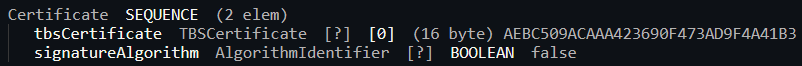
\includegraphics[width=\linewidth]{decode-smdpSigned2.png}
\caption{Decodifica del campo smdpSigned2 di authenticateClientResponse.}
\label{fig:decode-smdpSigned2}
\end{figure}

\subsection{Analisi di getBoundProfilePackage}
La figura \ref{fig:msg5-stream-pcap} mostra il contenuto del terzo messaggio inviato dal client (getBoundProfilePackage).\\
\begin{figure}
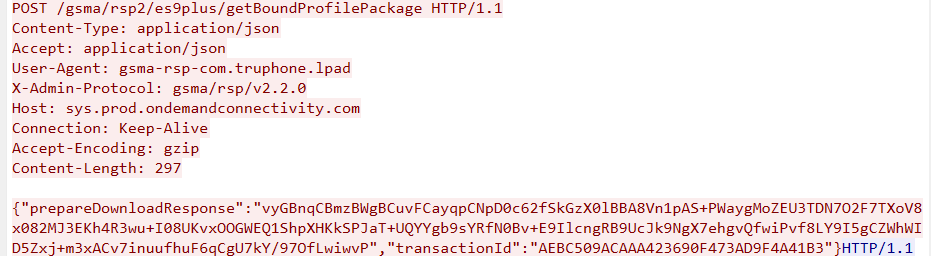
\includegraphics[width=\linewidth]{msg5-stream-pcap.png}
\caption{Messaggio di getBoundProfilePackage visualizzato su Wireshark.}
\label{fig:msg5-stream-pcap}
\end{figure}
Il payload è composto da due campi:
\begin{itemize}
\item \textbf{prepareDownloadResponse}: è una struttura dati in base64 che verrà descritta a breve;
\item \textbf{transactionId}: è il solito ID di transazione.
\end{itemize}
Qui di seguito si ha la definizione di prepareDownloadResponse \cite{RSP-definitions}.\\

\textit{PrepareDownloadResponse ::= [33] CHOICE \{ \textcolor{gray}{{-}{-} Tag `BF21'}}

\hspace{0.75cm} \textit{downloadResponseOk PrepareDownloadResponseOk,}

\hspace{0.75cm} \textit{downloadResponseError PrepareDownloadResponseError}

\textit{\}\\}

\textit{PrepareDownloadResponseOk ::= SEQUENCE \{}

\hspace{0.75cm} \textit{euiccSigned2 EUICCSigned2, \textcolor{gray}{{-}{-} Signed information}}

\hspace{0.75cm} \textit{euiccSignature2 [APPLICATION 55] OCTET STRING \textcolor{gray}{{-}{-} tag `5F37'}}

\textit{\}\\}

\textit{EUICCSigned2 ::= SEQUENCE \{}

\hspace{0.75cm} \textit{transactionId [0] TransactionId,}

\hspace{0.75cm} \textit{euiccOtpk [APPLICATION 73] OCTET STRING, \textcolor{gray}{{-}{-} otPK.EUICC.ECKA, tag `5F49'}}

\hspace{0.75cm} \textit{hashCc Octet32 OPTIONAL \textcolor{gray}{{-}{-} Hash of confirmation code}}

\textit{\}\\}

\noindent Anche prepareDownloadResponse, come authenticateServerResponse nel messaggio authenticateClient, si articola in due casi: prepareDownloadResponseOk nel caso in cui tutti i controlli effettuati dal client alla ricezione di authenticateClientResponse abbiano avuto successo, e prepareDownloadResponseError in caso contrario. La struttura dati prepareDownloadResponseError, in modo perfettamente analogo ad authenticateResponseError, è composta dall'ID di transazione e da un codice di errore.\\
D'altra parte, prepareDownloadResponseOk è composto dalla struttura dati euiccSigned2 e dalla relativa digital signature euiccSignature2, dove euiccSigned2 è composto a sua volta da:
\begin{itemize}
\item \textbf{transactionId}: è l'ID di transazione;
\item \textbf{euiccOtpk}: è la chiave pubblica otPK.EUICC.KA (sezione \ref{sec:keys});
\item \textbf{hashCc}: è un campo opzionale che è presente se il Confirmation Code è richiesto e corrisponde al valore SHA256(SHA256(Confirmation Code) $\vert$ transactionID).
\end{itemize}

\subsection{Analisi di getBoundProfilePackageResponse}
La figura \ref{fig:msg6-stream-pcap} mostra il contenuto della risposta del server al terzo messaggio inviato dal client (getBoundProfilePackageResponse).\\
\begin{figure}
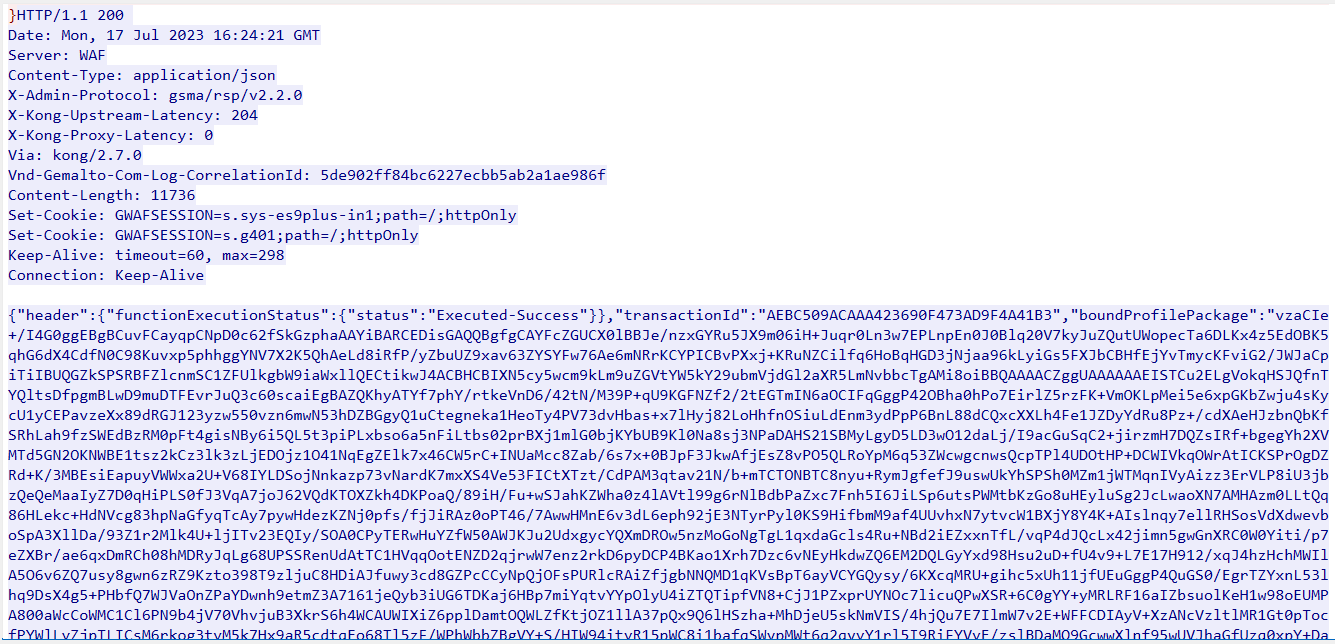
\includegraphics[width=\linewidth]{msg6-stream-pcap.png}
\caption{Messaggio di getBoundProfilePackageResponse visualizzato su Wireshark.}
\label{fig:msg6-stream-pcap}
\end{figure}
Il payload è composto dai seguenti tre campi:
\begin{itemize}
\item \textbf{header}: contiene ancora una volta \textit{\{``status":``Executed-Success"\}};
\item \textbf{transactionId}: è l'ID di transazione;
\item \textbf{boundProfilePackage}: è un campo codificato in base64 ed è molto grande, tant'è vero che non rientra per intero nella figura \ref{fig:msg6-stream-pcap}.
\end{itemize}
\begin{figure}
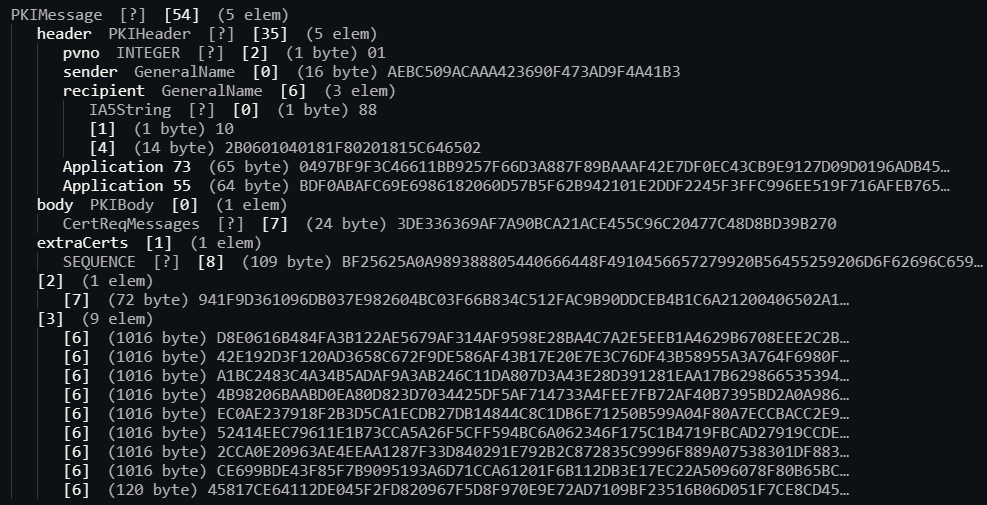
\includegraphics[width=\linewidth]{decode-boundProfilePackage.png}
\caption{Decodifica del campo boundProfilePackage di getBoundProfilePackageResponse.}
\label{fig:decode-boundProfilePackage}
\end{figure}
Com'è possibile osservare nella definizione riportata di seguito \cite{RSP-definitions}, il campo boundProfilePackage è composto da strutture di tipo TLV, ovvero sequenze di byte che a loro volta possono essere interpretate come elementi ASN.1 coi loro tag, le loro length e i loro value. Dalle figure \ref{fig:asn1-profileMetadata}, \ref{fig:decode-boundProfilePackage}, è possibile accorgersi che il campo sequenceOf88 di boundProfilePackage, che in questo caso specifico corrisponde al campo da 109 byte, contiene una sequenza di byte che corrisponde all'intero TLV di profileMetadata. D'altra parte, il campo sequenceOf86, complice anche la sua dimensione, ha tutta l'aria di essere il vero e proprio payload (cifrato) del profilo target.\\

\textit{BoundProfilePackage ::= [54] SEQUENCE \{ \textcolor{gray}{{-}{-} Tag `BF36'}}

\hspace{0.75cm} \textit{initialiseSecureChannelRequest [35] InitialiseSecureChannelRequest, \textcolor{gray}{{-}{-} Tag `BF23'}}

\hspace{0.75cm} \textit{firstSequenceOf87 [0] SEQUENCE OF [7] OCTET STRING, \textcolor{gray}{{-}{-} sequence of `87' TLVs}}

\hspace{0.75cm} \textit{sequenceOf88 [1] SEQUENCE OF [8] OCTET STRING, \textcolor{gray}{{-}{-} sequence of `88' TLVs}}

\hspace{0.75cm} \textit{secondSequenceOf87 [2] SEQUENCE OF [7] OCTET STRING OPTIONAL,}

\hspace{0.75cm} \textit{sequenceOf86 [3] SEQUENCE OF [6] OCTET STRING \textcolor{gray}{{-}{-} sequence of `86' TLVs}}

\textit{\}\\}

\subsection{Analisi di handleNotification}
Nelle due tracce diverse da quella di riferimento sono stati catturati anche dei messaggi di handleNotification inviati al server SM-DP+ da parte dell'LPA. Può tornare utile analizzarne un campione, come quello riportato in figura \ref{fig:msg7-stream-pcap}.\\
Si ha un solo campo JSON, pendingNotification, la cui definizione è mostrata qui di seguito.\\

\textit{PendingNotification ::= CHOICE \{}

\hspace{0.75cm} \textit{profileInstallationResult [55] ProfileInstallationResult, \textcolor{gray}{{-}{-} Tag `BF37'}}

\hspace{0.75cm} \textit{otherSignedNotification OtherSignedNotification}

\textit{\}\\}

\textit{OtherSignedNotification ::= SEQUENCE \{}

\hspace{0.75cm} \textit{tbsOtherNotification NotificationMetadata,}

\hspace{0.75cm} \textit{euiccNotificationSignature [APPLICATION 55] OCTET STRING, \textcolor{gray}{{-}{-} eUICC signature}}

\hspace{0.75cm} \textit{euiccCertificate Certificate, \textcolor{gray}{{-}{-} CERT.EUICC.ECDSA}}

\hspace{0.75cm} \textit{eumCertificate Certificate \textcolor{gray}{{-}{-} CERT.EUM.ECDSA}}

\textit{\}\\}

\textit{ProfileInstallationResult ::= [55] SEQUENCE \{ \textcolor{gray}{{-}{-} Tag `BF37'}}

\hspace{0.75cm} \textit{profileInstallationResultData [39] ProfileInstallationResultData,}

\hspace{0.75cm} \textit{euiccSignPIR EuiccSignPIR}

\textit{\}\\}

\textit{ProfileInstallationResultData ::= [39] SEQUENCE \{ \textcolor{gray}{{-}{-} Tag `BF27'}}

\hspace{0.75cm} \textit{transactionId[0] TransactionId, \textcolor{gray}{{-}{-} The Transaction ID generated by the SM-DP+}}

\hspace{0.75cm} \textit{notificationMetadata [47] NotificationMetadata,}

\hspace{0.75cm} \textit{smdpOid OBJECT IDENTIFIER, \textcolor{gray}{{-}{-} SM-DP+ OID}}

\hspace{0.75cm} \textit{finalResult [2] CHOICE \{}

\hspace{1.5cm} \textit{successResult SuccessResult,}

\hspace{1.5cm} \textit{errorResult ErrorResult}

\hspace{0.75cm} \textit{\}}

\textit{\}\\}

\textit{SuccessResult ::= SEQUENCE \{}

\hspace{0.75cm} \textit{aid [APPLICATION 15] OCTET STRING (SIZE (5..16)), \textcolor{gray}{{-}{-} AID of ISD-P}}

\hspace{0.75cm} \textit{simaResponse OCTET STRING \textcolor{gray}{{-}{-} contains (multiple) `EUICCResponse'}}

\textit{\}\\}

\textit{ErrorResult ::= SEQUENCE \{}

\hspace{0.75cm} \textit{bppCommandId BppCommandId,}

\hspace{0.75cm} \textit{errorReason ErrorReason,}

\hspace{0.75cm} \textit{simaResponse OCTET STRING OPTIONAL \textcolor{gray}{{-}{-} contains (multiple) `EUICCResponse'}}

\textit{\}\\}

\begin{figure}
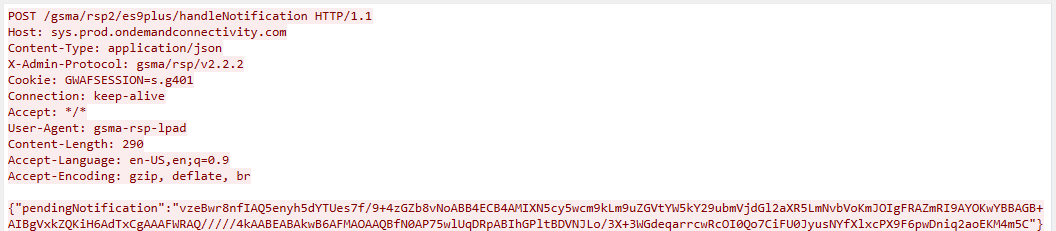
\includegraphics[width=\linewidth]{msg7-stream-pcap.png}
\caption{Messaggio di handleNotification visualizzato su Wireshark.}
\label{fig:msg7-stream-pcap}
\end{figure}

\noindent Si hanno due casi possibili: pendingNotification pari alla struttura dati profileInstallationResult e pendingNotification pari alla struttura dati otherSignedNotification.
\begin{itemize}
\item Nel primo caso, si ha una struttura profileInstallationResultData composta da ID di transazione, alcuni metadati di notificazione, OID (i.e. l'identificatore) del server SM-DP+ ed esito finale dell'installazione del profilo all'interno dell'eUICC (che può essere un successResult o un errorResult). Oltre a profileInstallationResultData, il campo pendingNotification è composto anche da euiccSignPIR, che risulta essere la signature di profileInstallationResultData.
\item Nel secondo caso, invece, si hanno alcuni metadati di notificazione, la relativa digital signature, il certificato dell'eUICC (CERT.EUICC.SIG) e il certificato dell'EUM (CERT.EUM.SIG). Intuitivamente, si ricade in questa casistica in contesti differenti da quello in cui l'LPA ha bisogno di comunicare l'esito dell'installazione del profilo (i.e. il successResult o l'errorResult).
\end{itemize}
Poiché, com'è stato già visto, la struttura dei certificati è piuttosto grande e poiché la stringa in base64 che codifica il campo pendingNotification del messaggio handleNotification, al contrario, è molto breve, è già possibile intuire che il messaggio catturato nella traccia ricada nel primo caso esposto precedentemente, dove pendingNotification è pari alla struttura dati profileInstallationResult che, verosimilmente, contiene un successResult. Tale intuizione trova conferma in figura \ref{fig:decode-pendingNotification} tratta dal sito \textit{ASN.1 JavaScript decoder}, dove chiaramente non compaiono riferimenti a certificati.
\begin{figure}
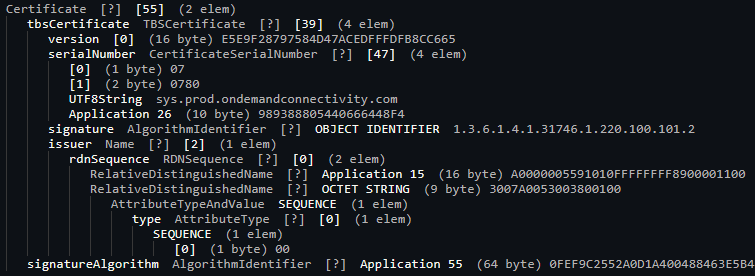
\includegraphics[width=\linewidth]{decode-pendingNotification.png}
\caption{Decodifica del campo pendingNotification di handleNotification.}
\label{fig:decode-pendingNotification}
\end{figure}

\section{Implementazione dei simulatori}
Il sistema di simulazione sviluppato è un'applicazione Python composta da tre moduli principali:
\begin{itemize}
\item \textbf{rootCA}: è il modulo relativo al Certificate Issuer. È composto unicamente da un eseguibile per la generazione di certificati custom;
\item \textbf{smdp}: è il modulo relativo al server SM-DP+. È composto a sua volta da:
\begin{itemize}
\item un eseguibile per la generazione di certificati custom;
\item un eseguibile per la comunicazione con l'operatore per il rilascio di un nuovo profilo;
\item un eseguibile per le procedure di Common Mutual Authentication e di download e installazione del profilo;
\item un file per tenere traccia delle informazioni sui profili esistenti che sono il Matching ID, l'EID dell'eUICC a cui il profilo è destinato, l'ICCID, il numero di tentativi di download effettuati, l'ID dell'eventuale transazione in cui si sta tentando correntemente di installare il profilo, lo stato attuale del profilo, il tipo di profilo e l'eventuale Confirmation Code che serve per fornire la conferma finale sul download del profilo;
\item un eseguibile per effettuare il clean-up del file di cui sopra, in modo tale da lasciare esclusivamente i profili in uno stato diverso da `Released' e da `Error'.
\item un eseguibile per generare il QR code associato al profilo con un dato Matching ID.
\end{itemize}
\item \textbf{euicc}: è il modulo che comprende la coppia eUICC + LPA e l'operatore telefonico. Questo accorpamento consente di semplificare la logica applicativa lato client e di bypassare, ad esempio, la comunicazione tra l'operatore e l'LPA che si ha nella fase di download initialization (sezione \ref{sec:step-RSP}). Tale modulo è composto a sua volta da:
\begin{itemize}
\item un eseguibile per la generazione di certificati custom sia per l'eUICC che per l'EUM;
\item un eseguibile per la comunicazione col server SM-DP+ per il rilascio di un nuovo profilo (qui l'attore impersonificato è l'operatore);
\item un eseguibile per le procedure di Common Mutual Authentication e di download e installazione del profilo (qui l'attore impersonificato è la coppia eUICC + LPA);
\item un file che rappresenta una RAT.
\end{itemize}
\end{itemize}

\subsection{Librerie Python utilizzate}
La tabella \ref{tab:libraries} racchiude tutte le librerie Python che sono state sfruttate per il sistema simulato e i relativi utilizzi.\\
\begin{table}[h!]
\begin{center}
\captionsetup{skip=4pt}
\caption{Librerie Python utilizzate.}
\label{tab:libraries}
\begin{tabularx}{\textwidth}{|c|X|}
\hline
\textbf{Libreria} & \textbf{Utilizzo}\\
\hline
asn1crypto & Viene usata a supporto della generazione e della verifica delle signature.\\
\hline
asn1tools & È la libreria di riferimento per convertire i dati in e dal formato ASN.1; prevede l'ausilio di alcuni file contenenti, tra le varie cose, le definizioni ASN.1 che vengono usate \cite{RSP-definitions}.\\
\hline
base64 & Viene usata per convertire i dati in e dal formato base64.\\
\hline
cryptography & Viene usata a supporto della generazione dei certificati custom, della generazione e della verifica delle signature e di altre funzionalità crittografiche.\\
\hline
datetime & Viene usata per definire delle date o degli istanti di tempo; è utile ad esempio per inizializzare i campi \textit{not valid before} e \textit{not valid after} dei certificati custom.\\
\hline
gzip & Viene usata per estrarre il payload dei messaggi eventualmente compressi del server SM-DP+ (non è il caso di Very Mobile).\\
\hline
hashlib & Viene usata per generare fingerprint ad esempio con la funzione hash SHA256().\\
\hline
http & Viene sfruttata per utilizzare la parte client e/o la parte server per la comunicazione HTTP.\\
\hline
json & Viene usata per convertire i dati in e dal formato JSON, oltre che per leggere e scrivere sui file .json.\\
\hline
os & Viene usata per interagire col sistema operativo.\\
\hline
random & Viene usata per generare valori o stringhe in modo pseudo-randomico, come ad esempio i Matching ID.\\
\hline
requests & Viene usata in alternativa alla libreria http, in particolar modo per utilizzare la parte client per la comunicazione HTTP quando si ha a che fare con un server che con la libreria http dà problemi.\\
\hline
secrets & Viene usata per generare sequenze di byte pseudo-randomiche, come ad esempio le challenge.\\
\hline
signal & Viene usata per definire un timeout ove è previsto un input da parte dell'utente da immettere entro un tempo limitato.\\
\hline
six & Viene usata per verificare se determinate variabili sono istanze di uno specifico tipo di dato.\\
\hline
socket & Viene usata per definire e utilizzare le socket dalle quali verrà istanziata la connessione HTTP.\\
\hline
ssl & Viene usata per aggiungere la componente SSL (o TLS) alla connessione HTTP.\\
\hline
sslkeylog & Viene usata per generare un log su ciò che avviene all'interno di una connessione di rete.\\
\hline
string & Viene usata per la definizione di stringhe o di insiemi di caratteri; ad esempio, può indicare il set dei possibili caratteri che potenzialmente comporranno una stringa pseudo-randomica.\\
\hline
sys & Viene usata per interagire con l'ambiente runtime di Python.\\
\hline
\end{tabularx}
\end{center}
\end{table}

\subsection{Confronto tra specifiche GSMA e simulatori}
Per quanto concerne i dettagli implementativi del sistema simulato, è stato possibile formattare i messaggi scambiati tra le controparti in modo perfettamente compatibile con le specifiche di GSMA sia grazie al livello di dettaglio fornito dalle specifiche stesse \cite{GSMA-docs-new}, sia grazie alla completezza delle definizioni ASN.1 per il protocollo RSP \cite{RSP-definitions}, anche se è stato necessario ritoccare queste ultime con piccole correzioni al fine di ottenere un funzionamento corretto. Un aspetto sicuramente più interessante da trattare riguarda i controlli che devono essere effettuati dalle controparti a ogni messaggio ricevuto.

\subsubsection{Check da parte del server alla ricezione di initiateAuthetication}
\begin{itemize}
\item Validità dell'indirizzo SM-DP+: l'implementazione prevede un controllo su se l'hostname specificato è uguale al vero hostname del server.
\item Validità del contenuto di euiccInfo1: l'implementazione prevede un controllo su se in euiccCiPKIdListForVerification e in euiccCiPKIdListForSigning compare il valore di euiccCiPKIdToBeUsed.
\end{itemize}

\subsubsection{Check da parte dell'LPA alla ricezione di initiateAuthenticationResponse}
\begin{itemize}
\item Validità dell'OID (opzionale): non implementato.
\item Validità dell'indirizzo SM-DP+: l'implementazione prevede un controllo su se l'hostname ricevuto corrisponde a quello inviato nel precedente messaggio di initiateAuthentication.
\item Validità della chiave pubblica del Root della certificate chain (opzionale): non implementato.
\item Eventuali altri controlli previsti per l'LPA non sono implementati.
\end{itemize}

\subsubsection{Check da parte dell'eUICC alla ricezione di initiateAuthenticationResponse}
\begin{itemize}
\item Validità della catena di certificati: l'implementazione prevede un controllo sul certificato CERT.DPauth.SIG mediante la chiave pubblica del CI (i.e. del Root).
\item Validità di serverSignature1: l'implementazione prevede un controllo della signature contenuta nel messaggio mediante la chiave pubblica associata al certificato CERT.DPauth.SIG.
\item Validità di euiccChallenge: l'implementazione prevede un controllo su se l'euiccChallenge ricevuta corrisponde a quella inviata nel precedente messaggio di initiateAuthentication.
\item Supporto della chiave pubblica del CI ricevuta nel campo euiccCiPKIdToBeUsed: l'implementazione prevede un controllo su se euiccCiPKIdToBeUsed è incluso all'interno del campo euiccCiPKIdListForSigning.
\item Validità della CRL (opzionale): non implementato.
\end{itemize}
È stato aggiunto anche un controllo su se il campo transactionId di initiateAuthenticationResponse corrisponde al sotto-campo transactionId della struttura serverSigned1 contenuta nel medesimo messaggio.

\subsubsection{Check da parte del server alla ricezione di authenticateClient}
\begin{itemize}
\item Validità dell'ID di transazione: l'implementazione prevede un controllo su se il campo transactionId di authenticateClient e il sotto-campo transactionId della struttura euiccSigned1 sono uguali all'ID di transazione originariamente comunicato dal server.
\item Validità del Root della certificate chain usata dal client: l'implementazione prevede un controllo su se il campo \textit{AuthorityKeyIdentifier} del certificato CERT.EUM.SIG corrisponde alla variabile euiccCiPKIdToBeUsed.
\item Validità della catena di certificati: l'implementazione prevede un controllo sul certificato CERT.EUM.SIG mediante la chiave pubblica del CI, ma anche un controllo sul certificato CERT.EUICC.SIG mediante la chiave pubblica dell'EUM.
\item Validità di euiccSignature1: l'implementazione prevede un controllo della signature contenuta nel messaggio mediante la chiave pubblica associata al certificato CERT.EUICC.SIG.
\item Validità di serverChallenge: l'implementazione prevede un controllo su se la serverChallenge ricevuta corrisponde a quella inviata nel precedente messaggio di initiateAuthenticationResponse.
\item Validità del Matching ID: l'implementazione prevede un controllo su se il campo matchingId della struttura ctxParams1 corrisponde a un Matching ID realmente esistente per il server e correntemente nello stato `Released' o `Download'.
\end{itemize}
A livello implementativo sono stati aggiunti anche i controlli elencati qui di seguito.
\begin{itemize}
\item Validità dell'indirizzo SM-DP+: si ha un controllo su se il campo serverAddress della struttura euiccSigned1 è uguale all'hostname del server.
\item Validità dei campi di euiccInfo2 in comune con euiccInfo1: si ha un controllo su se i campi svn, euiccCiPKIdListForVerification ed euiccCiPKIdListForSigning assumono gli stessi valori in euiccInfo2 all'interno di authenticateClient e in euiccInfo1 all'interno di initiateAuthentication.
\end{itemize}

\subsubsection{Check da parte dell'LPA alla ricezione di authenticateClientResponse}
\begin{itemize}
\item Verifica della RAT: l'implementazione prevede una funzione che segue la logica introdotta nella sezione \ref{sec:rat}.
\item Conferma da parte dell'utente: l'implementazione prevede due casi. Nel primo caso è richiesta l'acquisizione del Confirmation Code da parte dell'utente e, se questo è errato o scatta il timeout, viene invocata la procedura di Common Cancel Session. Nel secondo caso è richiesta la conferma semplice e, se l'utente risponde `No', `Not now' oppure fa scadere il timeout, viene invocata la procedura di Common Cancel Session.
\end{itemize}

\subsubsection{Check da parte dell'eUICC alla ricezione di authenticateClientResponse}
\begin{itemize}
\item Validità di CERT.DPpb.SIG: l'implementazione prevede un controllo su CERT.DPpb.SIG mediante la chiave pubblica del CI.
\item Appartenenza di CERT.DPpb.SIG e di CERT.DPauth.SIG alla medesima entità: l'implementazione prevede un controllo su se l'Organization Name di CERT.DPpb.SIG corrisponde all'Organization Name di CERT.DPauth.SIG, e un controllo su se l'Organization Name dell'issuer di CERT.DPpb.SIG corrisponde all'Organization Name dell'issuer di CERT.DPauth.SIG.
\item Validità di smdpSignature2: l'implementazione prevede un controllo della signature contenuta nel messaggio mediante la chiave pubblica associata al certificato CERT.DPpb.SIG.
\item Validità dell'ID di transazione: l'implementazione prevede un controllo su se il campo transactionId di authenticateClientResponse e il sotto-campo transactionId della struttura smdpSigned2 sono uguali all'ID di transazione che identifica la sessione RSP corrente.
\end{itemize}
È stato aggiunto anche un controllo su se i campi serviceProviderName e profileName della struttura profileMetadata corrispondono a stringhe non vuote.

\subsubsection{Check da parte del server alla ricezione di getBoundProfilePackage}
\begin{itemize}
\item Validità di euiccSignature2: l'implementazione prevede un controllo della signature contenuta nel messaggio mediante la chiave pubblica associata al certificato CERT.EUICC.SIG.
\item Validità del Confirmation Code (opzionale): l'implementazione prevede un controllo sull'hash del Confirmation Code ricevuto dal server; se il check non va a buon fine, è previsto un incremento del contatore dei tentativi di immissione del codice e un controllo su se il contatore ha sforato il numero massimo ammissibile.
\end{itemize}
È stato aggiunto anche un controllo su se il campo transactionId di getBoundProfilePackage e il sotto-campo transactionId della struttura euiccSigned2 sono uguali all'ID di transazione che identifica la sessione RSP corrente.

\subsubsection{Check da parte del client alla ricezione di getBoundProfilePackageResponse}
In questa fase, è stato deciso di sintetizzare tutti i check svolti da parte dell'LPA e dell'eUICC in cinque punti fondamentali.
\begin{itemize}
\item Validità del Bound Profile Package: l'implementazione prevede un controllo in modo particolare sul campo sequenceOf88 della struttura boundProfilePackage per verificare se corrisponde alla codifica ASN.1 dell'intero campo profileMetadata ricevuto nel precedente messaggio del server (authenticateClientResponse).
\item Validità del Remote Operation Type: l'implementazione prevede un controllo su se il campo remoteOpId della struttura initialiseSecureChannelRequest corrisponde a un'operazione remota (Remote Operation) supportata.
\item Validità dell'ID di transazione: l'implementazione prevede un controllo su se il campo transactionId di getBoundProfilePackageResponse e il sotto-campo transactionId della struttura initialiseSecureChannelRequest sono uguali all'ID di transazione che identifica la sessione RSP corrente.
\item Validità della Profile Class: l'implementazione prevede un controllo su se la classe del profilo target (Profile Class) è supportata.
\item Validità di smdpSign: l'implementazione prevede un controllo della signature contenuta nella struttura initialiseSecureChannelRequest del messaggio mediante la chiave pubblica associata al certificato CERT.DPpb.SIG.
\end{itemize}

\subsubsection{Check da parte del server alla ricezione di handleNotification}
Nonostante la sezione \ref{sec:down-confirm} non parli esplicitamente di controlli effettuati dal server SM-DP+ dopo la ricezione del messaggio handleNotification da parte dell'LPA, si è comunque deciso di inserire due check che sembravano ormai ovvi e doverosi.
\begin{itemize}
\item Validità dell'ID di transazione: l'implementazione prevede un controllo su se il campo transactionId della struttura profileInstallationResultData è uguale all'ID di transazione che identifica la sessione RSP corrente.
\item Validità di euiccSignPIR: l'implementazione prevede un controllo della signature contenuta nel messaggio mediante la chiave pubblica associata al certificato CERT.EUICC.SIG.
\end{itemize}

\subsubsection{Check da parte del server alla ricezione di cancelSession}
All'interno del sistema simulato, il client avvia la procedura di Common Cancel Session nei casi riportati qui di seguito, come suggerito dalle specifiche di GSMA \cite{GSMA-docs-new}:
\begin{itemize}
\item il messaggio authenticateClientResponse da parte del server contiene un solo campo (transactionId);
\item il messaggio authenticateClientResponse contiene la struttura profileMetadata con serviceProviderName o profileName pari alla stringa vuota;
\item fallisce un qualche controllo sulle Profile Policy Rules all'interno dei metadati del profilo (struttura profileMetadata);
\item l'end user non inserisce correttamente in input l'eventuale Confirmation Code o comunque non fornisce la conferma sul download del profilo target;
\item il campo sequenceOf88 della struttura boundProfilePackage all'interno del messaggio getBoundProfilePackageResponse non corrisponde alla codifica ASN.1 dell'intero campo profileMetadata del precedente messaggio di authenticateClientResponse.
\end{itemize}
Quando il server riceve un messaggio di cancelSession all'interno del sistema simulato, vengono implementati i seguenti check:
\begin{itemize}
\item Validità dell'ID di transazione: l'implementazione prevede un controllo su se il campo transactionId di cancelSession e il sotto-campo transactionId della struttura euiccCancelSessionSigned sono uguali all'ID di transazione che identifica una sessione RSP correntemente attiva.
\item Validità di euiccCancelSessionSignature: l'implementazione prevede un controllo della signature contenuta nel messaggio mediante la chiave pubblica associata a CERT.EUICC.SIG.
\end{itemize}
L'unico aspetto da puntualizzare è la mancanza di un controllo sull'OID.

\section{Validazione dei simulatori}
Prima di sfruttare i simulatori implementati per condurre gli esperimenti successivi, è necessario dimostrare che essi siano corretti, assicurandosi che rispettino fedelmente le specifiche di GSMA, siano privi di bug e siano in grado di comunicare con successo con server e client reali. In altre parole, si vuole validare i simulatori.

\subsection{Validazione del simulatore lato client}
Per validare il simulatore del client, si è deciso di farlo comunicare con un server di test, ovvero un server SM-DP+ che non è stato concepito per rilasciare profili reali a utenti che vogliono ottenere un vero e proprio piano tariffario, bensì per effettuare delle prove e rilasciare quindi dei profili di test. Tipicamente, un server di test prevede l'utilizzo di catene di certificati di test, le più importanti delle quali vengono definite e messe a disposizione direttamente dalla GSMA \cite{GSMA-test-cert}. Si tratta di due catene di certificati insieme alle quali è possibile scaricare anche le relative chiavi pubbliche e chiavi private. Inoltre, tali certificati coprono tutte le entità coinvolte nella catena, dalla RootCA, al server SM-DP+, all'EUM, all'eUICC. La prima certificate chain, indicata con BRP, fa uso dell'algoritmo Brainpool, che è un algoritmo utilizzato nell'ambito della crittografia basata sulle curve ellittiche \cite{RFC-5639}, mentre la seconda, indicata con NIST, no.\\
Per aiutarsi con l'attività di debugging durante il processo di validazione del simulatore lato client, si è deciso di sfruttare un server di test open-source: \textbf{Osmo-smdpp}, che è possibile trovare su GitHub al link https://github.com/osmocom/pysim, ed è stato l'unico server SM-DP+ open-source reperibile al momento della validazione del simulatore. Si tratta di un server di test attualmente incompleto. Infatti, ha implementate tutte le funzioni necessarie per la mutua autenticazione e per il download dei profili di prova ma non prevede ancora tutti i controlli che, secondo le specifiche di GSMA \cite{GSMA-docs-new}, un qualunque server SM-DP+ deve effettuare a ogni messaggio ricevuto da parte dell'LPA coinvolta nella comunicazione; ciò è confermato dal fatto che all'interno del codice di Osmo-smdpp vi è un'ingente quantità di commenti marcati con l'espressione \textit{TODO}. Comunque sia, per semplicità, si è assunto che tale server di test fosse sufficiente per debuggare, completare e validare il simulatore del client appena sviluppato.\\
Il simulatore è stato approvato, e quindi considerato valido, nel momento in cui è stato in grado di completare con successo la comunicazione col server Osmo-smdpp inviando nell'ordine i messaggi initiateAuthentication, authenticateClient, getBoundProfilePackage e handleNotification, potendo sfruttare sia la catena di certificati BRP, sia la catena di certificati NIST.

\subsection{Validazione del simulatore lato server}
Per validare il simulatore del server, si è deciso di farlo comunicare con un client di test, che è composto da un'eUICC programmabile della Sysmocom. Tale eUICC può essere acquistata al sito https://shop.sysmocom.de e può essere inserita all'interno di un apposito lettore di SIM, il quale è direttamente collegabile al computer con cui si sta lavorando grazie al suo attacco USB ed è riportato in figura \ref{fig:eUICC-reader}. Inoltre, l'eUICC è pensata per comunicare col server di Osmocom (Osmo-smdpp) e, per questa ragione, supporta anch'essa la catena di certificati di test definita dalla GSMA, in particolare la NIST, che non fa uso dell'algoritmo Brainpool.\\
Per testare il simulatore del server, è stato sufficiente installare e compilare un'apposita LPA di test (\textbf{lpac}) reperibile su GitHub al link https://github.com/estkme-group/lpac, collegare al computer il lettore di SIM con all'interno l'eUICC programmabile e avviare sia il simulatore del server che LPA di test in modo tale da farli comunicare tra loro.\\
Il simulatore viene considerato valido nel momento in cui si riesce a installare con successo il profilo da lui offerto all'interno della SIM programmabile. Tuttavia, almeno per il momento, l'attività di debugging non ha consentito di raggiungere questo risultato: allo stato attuale, il simulatore è in grado di scambiare tutti i messaggi col client di test ma, dopo aver ricevuto il Bound Profile Package nel messaggio getBoundProfilePackageResponse, fornisce l'errore \textit{scp03tSecurityError} e non installa effettivamente il profilo all'interno dell'eUICC programmabile. Per questo motivo, il simulatore del server risulta validato solo parzialmente ma, grazie alla capacità di portare a termine la comunicazione coi client, rimane comunque uno strumento sufficientemente adeguato per intraprendere lo studio successivo con i client reali.
\begin{figure}
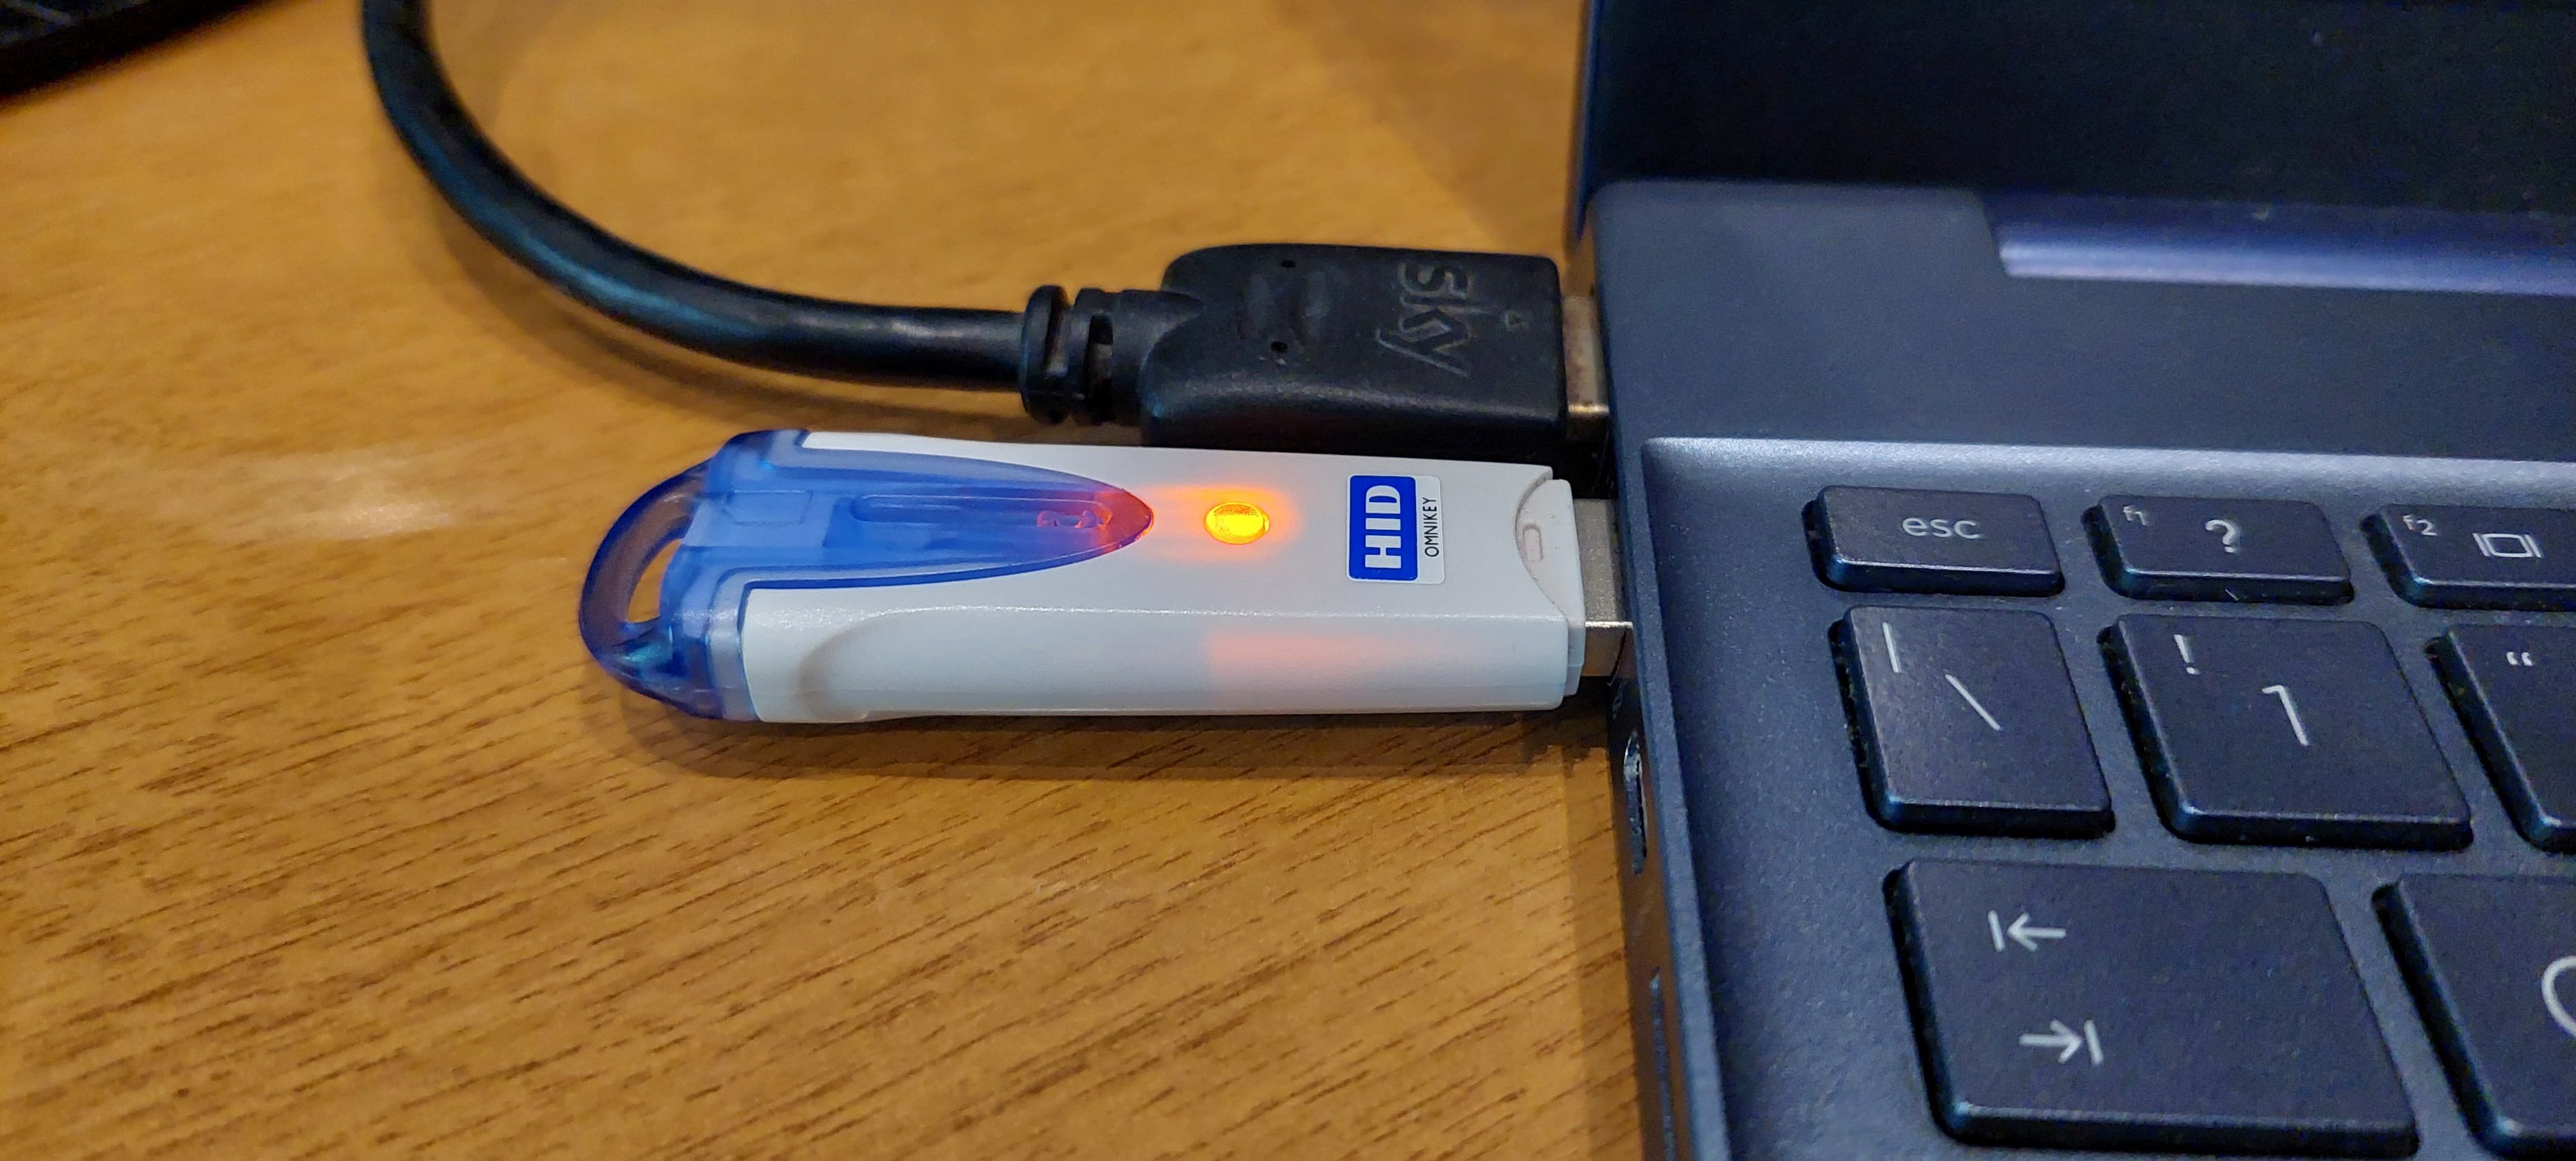
\includegraphics[width=\linewidth]{eUICC-reader.png}
\caption{Lettore di SIM utilizzato per validare il simulatore del server.}
\label{fig:eUICC-reader}
\end{figure}

\chapter{Analisi di sicurezza dell'eSIM}
\section{Descrizione dell'analisi}
L'analisi di sicurezza che ci si propone di effettuare si articola in due fasi.
\begin{enumerate}
\item Si individua un campione di server SM-DP+ da testare e, mediante il simulatore del client precedentemente sviluppato, si tenta di comunicare con ciascuno di loro in svariati modi diversi (e.g. modificando qualche campo di un messaggio, cambiando la certificate chain utilizzata, cambiando l'ordine dei messaggi inviati), costruendo così altrettanti casi di test. Per ciascun caso di test si analizzano le risposte di ogni server SM-DP+ del campione, col fine ultimo di stabilire se esse sono perfettamente conformi alle specifiche oppure lasciano intendere che il server abbia omesso dei check, aprendo le porte a eventuali vulnerabilità.
\item Si utilizzano dei dispositivi mobili (i.e. coppie eUICC - LPA) per definire ulteriori casi di test a parti invertite. Così, sfruttando il simulatore del server implementato in precedenza, si tenta di comunicare coi dispositivi mobili e si raccolgono i loro messaggi di risposta per ciascun caso di test, anche qui con lo scopo di verificare se i loro eUICC e le loro LPA sono conformi alle specifiche.
\end{enumerate}

\section{Ottenimento dei server da testare}
L'idea originale consisteva nell'individuare tutti i server SM-DP+ del mondo in modo tale da effettuare dei test esaustivi e su larga scala. Tuttavia, non è stato possibile trovare in rete alcun riferimento a hostname o indirizzi IP dei server SM-DP+, eccezion fatta per i server di test e per alcuni server SM-DS. I server di test trovati sono quello di Google (con hostname \textit{prod.smdp-plus.rsp.goog}), Infineon (con hostname \textit{testsmdpplus.infineon.com}), Sysmocom (con hostname\\ \textit{smdpp.test.rsp.sysmocom.de}) e Truphone (con hostname \textit{rsp.truphone.com}). I server SM-DS trovati sono quello di GSMA (con hostname \textit{lpa.ds.gsma.com}), eSIM Discovery Production (con hostname \textit{lpa.live.esimdiscovery.com}), eSIM Discovery Staging (con hostname \textit{lpa.live.esimdiscovery.dev}), Stork (con hostname \textit{prod.smds.rsp.goog}) e Verizon Wireless (con hostname \textit{lpads.vzw.otgeuicc.com}). Tutti questi server, a differenza di Osmo-smdpp, non sono open-source e non devono essere installati sulla macchina locale per essere eseguiti, bensì possono essere visti come normali server SM-DP+.\\
Per trovare dei server SM-DP+ che siano affiliati a degli operatori e permettano realmente di effettuare il download di profili, è stato necessario procedere come per il server di Very Mobile (vedere capitolo 4), ovvero acquistare un piano tariffario reale su un telefono che supporta l'eSIM, ricavando così l'hostname del server SM-DP+ a partire da un'email ricevuta dall'operatore (come quella in figura \ref{fig:email}). Sono stati così individuati i seguent server SM-DP+:
\begin{itemize}
\item server di Iliad, con hostname \textit{frm.prod.ondemandconnectivity.com};
\item server di Tim, con hostname \textit{rsp-0001.oberthur.net};
\item server di Very Mobile, con hostname \textit{sys.prod.ondemandconnectivity.com}.
\end{itemize}
Successivamente, è stato effettuato un altro tentativo per ricavare l'hostname del maggior numero di server SM-DP+ possibile, che consiste nel provare a sfruttare l'indirizzo IP dei server già noti. In particolare, tramite il comando \textit{dig}, sono state inviate delle query a un server DNS con lo scopo di ottenere l'indirizzo IP associato a ciascun hostname ottenuto, compreso quello dei server di test. La tabella \ref{tab:IP-addr} mette insieme hostname e indirizzo IP dei server SM-DP+ attualmente noti.
\begin{table}[h!]
\begin{center}
\captionsetup{skip=4pt}
\caption{Hostname e indirizzo IP dei server SM-DP+ noti.}
\label{tab:IP-addr}
\begin{tabularx}{\textwidth}{|c|c|X|} % <-- Alignments: 1st column center and 2nd center, with vertical lines in between
\hline
\textbf{Nome} & \textbf{Hostname} & \textbf{Indirizzo IP}\\
\hline
Iliad & frm.prod.ondemandconnectivity.com & 34.107.65.70\\
\hline
Tim & rsp-0001.oberthur.net & 51.11.249.51\\
\hline
Very Mobile & sys.prod.ondemandconnectivity.com & 34.107.65.70\\
\hline
eSIM Disc. Production & lpa.live.esimdiscovery.com & 34.48.45.29\\
\hline
eSIM Disc. Staging & lpa.live.esimdiscovery.com & 35.245.56.247\\
\hline
GSMA & lpa.ds.gsma.com & 34.89.151.119\\
\hline
Stork & prod.smds.rsp.goog & 34.95.109.237\\
\hline
Verizon Wireless & lpads.vzw.otgeuicc.com & 35.245.232.18\\
\hline
Google & prod.smdp-plus.rsp.goog & 34.95.109.237\\
\hline
Infineon & testsmdpplus.infineon.com & 52.57.244.228; 18.196.185.236 \\
\hline
Sysmocom & smdpp.test.rsp.sysmocom.de & 213.95.46.137\\
\hline
Truphone & rsp.truphone.com & 185.99.24.88\\
\hline
\end{tabularx}
\end{center}
\end{table}

\begin{figure}
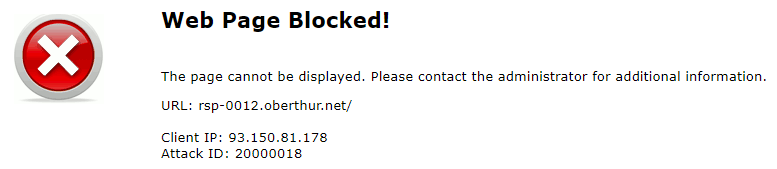
\includegraphics[width=\linewidth]{web-page-blocked.png}
\caption{Pagina web con cui rsp-0012.oberthur.net risponde.}
\label{fig:web-page-blocked}
\end{figure}
\noindent Dalla tabella \ref{tab:IP-addr} è possibile concludere che non c'è un pattern negli indirizzi IP dei server SM-DP+, per cui è impensabile ricavare ulteriori indirizzi IP a partire da quelli noti. Inoltre, è possibile osservare che gli operatori Iliad e Very Mobile si appoggiano sul medesimo server SM-DP+, così come Stork e Google.\\
Si potrebbe pensare di procedere con la forza bruta e, per ogni indirizzo IP che va da 0.0.0.0 a 255.255.255.255, provare a stabilire se esso è associato o meno a un server SM-DP. Tuttavia, né inviando query a un server DNS, né provando a contattare direttamente gli host specificando il loro indirizzo IP anziché il loro hostname si riescono a ottenere informazioni utili.\\
L'unico aspetto su cui si è potuto lavorare è l'hostname del server SM-DP+ associato a Tim, dove compare un numero $N$ a quattro cifre (0001). Facendo variare $N$, si ottengono ancora degli hostname esistenti e validi per qualunque $N$ a quattro cifre compreso tra 0001 e 0032. In particolare, i 32 hostname così trovati sono mappati soltanto su quattro indirizzi IP diversi, per cui molti di loro costituiscono degli alias. I quattro host individuati solo elencati di seguito:
\begin{itemize}
\item \textit{rsp-0001.oberthur.net}, con indirizzo IP 51.11.249.51;
\item \textit{rsp-0002.oberthur.net}, con indirizzo IP 51.11.249.55;
\item \textit{rsp-0003.oberthur.net}, con indirizzo IP 185.200.48.11;
\item \textit{rsp-0012.oberthur.net}, con indirizzo IP 213.39.85.20.
\end{itemize}
Stabilendo una prima connessione con ciascuno dei quattro host, è stato possibile capire che dietro gli hostname \textit{rsp-0001.oberthur.net} e \textit{rsp-0002.oberthur.net} si cela con ogni probabilità il medesimo server SM-DP+, poiché nei due casi ha esibito esattamente lo stesso certificato CERT.DPauth.SIG. Inoltre, dietro l'hotname \textit{rsp-0012.oberthur.net} si cela un server non più utilizzabile perché, indipendentemente dal messaggio di richiesta, risponde con l'errore ``Web Page Blocked!" come riportato in figura \ref{fig:web-page-blocked}. Perciò, ai fini degli esperimenti, oltre a \textit{rsp-0001.oberthur.net} (server di Tim), verrà considerato solo \textit{rsp-0003.oberthur.net}, che verrà identificato come `gemello del server di Tim'.\\
La tabella \ref{tab:all-servers} mostra tutti i server che verranno contattati durante l'esecuzione dei test.\\

\begin{table}[h!]
\begin{center}
\captionsetup{skip=4pt}
\caption{Elenco dei server SM-DP+ coinvolti negli esperimenti.}
\label{tab:all-servers}
\begin{tabularx}{\textwidth}{|c|X|X|} % <-- Alignments: 1nd column center, with vertical lines in between
\hline
\textbf{Nome} & \textbf{Descrizione} & \textbf{Note}\\
\hline
Iliad \& Very Mobile & Server SM-DP+ reale & Verrà contattato usando una certificate chain custom con CI = GSMA*.\\
\hline
Tim & Server SM-DP+ reale & Verrà contattato usando una certificate chain custom con CI = GSMA*.\\
\hline
Gemello di Tim & Server SM-DP+ reale & Verrà contattato usando una certificate chain custom con CI = GSMA*.\\
\hline
eSIM Disc. Production & Server SM-DS & Verrà contattato usando una certificate chain custom con CI = GSMA*.\\
\hline
eSIM Disc. Staging & Server SM-DS & Verrà contattato usando una certificate chain custom con CI = GSMA*.\\
\hline
GSMA & Server SM-DS & Verrà contattato usando una certificate chain custom con CI = GSMA*.\\
\hline
Verizon Wireless & Server SM-DS & Verrà contattato usando una certificate chain custom con CI = GSMA*.\\
\hline
Stork \& Google & Server SM-DS / SM-DP+ di test & Verrà contattato usando una certificate chain di test**. Matching ID: 052X-UFXS-CQIY-PNGL.\\
\hline
Infineon & Server SM-DP+ di test & Verrà contattato usando una certificate chain di test. Matching ID: ApcLl-k0Ulo-kqSlk-GLhCl.\\
\hline
Sysmocom & Server SM-DP+ di test & Verrà contattato usando una certificate chain di test. Matching ID: TS48v1\_A.\\
\hline
Truphone & Server SM-DP+ di test & Verrà contattato usando una certificate chain custom con CI = GSMA*. Matching ID: QR-G-5C-1LS-1W1Z9P7.\\
\hline
Osmo-smdpp & Server SM-DP+ di test open-source installato in locale & Verrà contattato usando una certificate chain di test. Matching ID: TS48v1\_A.\\
\hline
Simulatore & Simulatore lato server precedentemente implementato & Può essere contattato usando una certificate chain qualsiasi e un Matching ID custom.\\
\hline
\end{tabularx}
\end{center}
\end{table}
\noindent \textit{*Non è possibile disporre di un'intera certificate chain valida della GSMA assieme a tutte le chiavi private associate. È per questo motivo che il certificato presentato dal simulatore del client all'interno del messaggio authenticateClient non potrebbe essere considerato valido. Dunque, i successivi esperimenti non possono spingersi oltre alla procedura di Common Mutual Authentication.}\\ \\
\textit{**La certificate chain di test supportata dal server di Stork e Google è diversa da quella prevista dagli altri server di test.}

\section{Risposte dei server testati}
\subsection{Casi di test definiti}
I casi di test che sono stati implementati ed eseguiti ai fini della presente trattazione sono riportati nella tabella \ref{tab:servers-test-cases}.\\
\begin{table}[h!]
\begin{center}
\captionsetup{skip=4pt}
\caption{Elenco dei casi di test definiti per i server SM-DP+.}
\label{tab:servers-test-cases}
\begin{tabularx}{\textwidth}{|c|X|} % <-- Alignments: 1st column center, with vertical lines in between
\hline
\textbf{ID} & \textbf{Descrizione}\\
\hline
1 & Il simulatore del client si comporta perfettamente come da specifiche.\\
\hline
2 & Manomissione del messaggio authenticateClient: invio della struttura authenticateResponseError anziché authenticateResponseOk.\\
\hline
3 & Manomissione del messaggio authenticateClient: utilizzo di una certificate chain lato client differente da quella scelta di default.\\
\hline
4 & Manomissione del messaggio authenticateClient: calcolo errato dalla signature (euiccSignature1).\\
\hline
5.1 & Manomissione del messaggio authenticateClient (sotto-campo euiccInfo2): utilizzo di un SVN (Specification Version Number) non atteso (e.g. 0x000000, che corrisponderebbe alla versione 0.0.0).\\
\hline
5.2 & Manomissione del messaggio authenticateClient (sotto-campo euiccInfo2): utilizzo di euiccCiPKIdListForVerification ed euiccCiPKIdListForSigning non attesi (pur mantenendo la certificate chain di default).\\
\hline
5.3 & Manomissione del messaggio authenticateClient (sotto-campo euiccInfo2): sasAcreditationNumber = stringa vuota.\\
\hline
6.1 & Manomissione del messaggio authenticateClient (sotto-campo ctxParams1): eliminazione del sotto-campo imei.\\
\hline
6.2 & Manomissione del messaggio authenticateClient (sotto-campo ctxParams1): inserimento di un Matching ID non valido.\\
\hline
7.1 & Manomissione del messaggio authenticateClient: utilizzo di un Transaction ID non valido all'interno del campo euiccSigned1.\\
\hline
7.2 & Manomissione del messaggio authenticateClient: campo transactionId non valido direttamente all'interno di authenticateResponseOk.\\
\hline
8 & Manomissione del messaggio authenticateClient: utilizzo di un smdpAddress non valido all'interno del campo euiccSigned1.\\
\hline
9 & Manomissione del messaggio authenticateClient: utilizzo di una serverChallenge non valida all'interno del campo euiccSigned1.\\
\hline
10 & Manomissione del messaggio initiateAuthentication: utilizzo di una euiccChallenge malforme (e.g. 0x00).\\
\hline
11 & Manomissione del messaggio initiateAuthentication: utilizzo di un smdpAddress non valido.\\
\hline
12.1 & Manomissione del messaggio initiateAuthentication (campo euiccInfo1): utilizzo di un SVN (Specification Version Number) non atteso (e.g. 0x000000, che corrisponderebbe alla versione 0.0.0).\\
\hline
12.2 & Manomissione del messaggio initiateAuthentication (campo euiccInfo1): utilizzo di euiccCiPKIdListForVerification ed euiccCiPKIdListForSigning non attesi (pur mantenendo la certificate chain di default).\\
\hline
13.1 & Avvio della Common Cancel Session Procedure già dal primo messaggio.\\
\hline
13.2 & Avvio della Common Cancel Session Procedure a partire dal secondo messaggio.\\
\hline
14.1 & Invio di getBoundProfilePackage come primo messaggio.\\
\hline
14.2 & Invio di getBoundProfilePackage come secondo messaggio.\\
\hline
15 & Invio di getBoundProfilePackage come primo messaggio col campo transactionId pari all'ID di transazione di una connessione instaurata da un altro processo client messo appositamente in sleep.\\
\hline
\end{tabularx}
\end{center}
\end{table}

\subsubsection{Caso di test 1}
Consiste nel comunicare col server SM-DP+ seguendo fedelmente le specifiche, senza alcuna manomissione nel protocollo o nei messaggi inviati. Di seguito è descritto il comportamento dei server in esame in questo caso di test.
\begin{itemize}
\item \textbf{Iliad \& Very Mobile}: \textit{``status": ``Failed"} al secondo messaggio di risposta (authenticateClientResponse), con \textit{``subjectCode: ``1.2"}, \textit{``reasonCode": ``4.2"}, \textit{``subjectIdentifier": ``Function provider"}, \textit{``message": ``Internal error while verifying token signature: invalid Certificate Policies: [2.5.29.35, 2.23.146.1.2.1.2]"}.
\item \textbf{Tim}: \textit{``status": ``Failed"} al secondo messaggio di risposta (authenticateClientResponse), con \textit{``subjectCode: ``8.1.2"}, \textit{``reasonCode": ``6.1"}, \textit{``subjectIdentifier": ``EUM Certificate"}, \textit{``message": ``Verification Failed"}.
\item \textbf{Gemello di Tim}: \textit{``status": ``Failed"} al secondo messaggio di risposta (authenticateClientResponse), con \textit{``subjectCode: ``8.1.2"}, \textit{``reasonCode": ``6.1"}, \textit{``subjectIdentifier": ``EUM Certificate"}, \textit{``message": ``Verification Failed"}.
\item \textbf{eSIM Discovery Production}: HTTP\_INTERNAL\_SERVER\_ERROR (status code 500) al secondo messaggio di risposta (authenticateClientResponse).
\item \textbf{eSIM Discovery Staging}: HTTP\_INTERNAL\_SERVER\_ERROR (status code 500) al secondo messaggio di risposta (authenticateClientResponse).
\item \textbf{GSMA}: HTTP\_INTERNAL\_SERVER\_ERROR (status code 500) al secondo messaggio di risposta (authenticateClientResponse).
\item \textbf{Verizon Wireless}: HTTP\_INTERNAL\_SERVER\_ERROR (status code 500) al secondo messaggio di risposta (authenticateClientResponse).
\item \textbf{Stork \& Google}: \textit{``status": ``Failed"} al secondo messaggio di risposta (authenticateClientResponse), con \textit{``subjectCode: ``8.1.2"}, \textit{``reasonCode": ``6.1"}, \textit{``message": ``Execution Failed"} $\rightarrow$ la verifica del certificato dell'EUM non è andata a buon fine.
\item \textbf{Infineon}: HTTP\_BAD\_REQUEST (status code 400) al primo messaggio di risposta (initiateAuthenticationResponse).
\item \textbf{Sysmocom}: \textit{``status": ``Executed-Success"}.
\item \textbf{Truphone}: \textit{``status": ``Failed"} al secondo messaggio di risposta (authenticateClientResponse), con \textit{``subjectCode: ``8.1.2"}, \textit{``reasonCode": ``6.1"}, \textit{``subjectIdentifier": ``EUM Certificate"}, \textit{``message": ``Verification Failed"}.
\item \textbf{Osmo-smdpp}: \textit{``status": ``Executed-Success"}.
\item \textbf{Simulatore}: \textit{``status": ``Executed-Success"}.
\end{itemize}

\noindent Poiché il server Infineon dà problemi già dal primo messaggio (initiateAuthentication), non potrà essere oggetto dei casi di test che coinvolgono la manomissione del secondo messaggio (authenticateClient).

\subsubsection{Caso di test 2}
Consiste nel manomettere il messaggio authenticateClient inserendovi la struttura authenticateResponseError al posto di authenticateResponseOk, facendo credere al server SM-DP+ che la sua autenticazione non sia andata a buon fine.
\begin{itemize}
\item \textbf{Iliad \& Very Mobile}: HTTP\_NO\_CONTENT (status code 204) al secondo messaggio di risposta (authenticateClientResponse).
\item \textbf{Tim}: \textit{``status": ``Failed"} al secondo messaggio di risposta (authenticateClientResponse), con \textit{``subjectCode: ``8.8"}, \textit{``reasonCode": ``6.1"}, \textit{``subjectIdentifier": ``SMDP+"}, \textit{``message": ``Verification Failed"}.
\item \textbf{Gemello di Tim}: \textit{``status": ``Failed"} al secondo messaggio di risposta (authenticateClientResponse), con \textit{``subjectCode: ``8.8"}, \textit{``reasonCode": ``6.1"}, \textit{``subjectIdentifier": ``SMDP+"}, \textit{``message": ``Verification Failed"}.
\item \textbf{eSIM Discovery Production}: \textit{``status": ``Failed"} al secondo messaggio di risposta (authenticateClientResponse), con \textit{``subjectCode: ``8.1"}, \textit{``reasonCode": ``6.1"}, \textit{``subjectIdentifier": ``eUICC"}, \textit{``message": ``serverChallenge is invalid"}.
\item \textbf{eSIM Discovery Staging}: \textit{``status": ``Failed"} al secondo messaggio di risposta (authenticateClientResponse), con \textit{``subjectCode: ``8.1"}, \textit{``reasonCode": ``6.1"}, \textit{``subjectIdentifier": ``eUICC"}, \textit{``message": ``serverChallenge is invalid"}.
\item \textbf{GSMA}: \textit{``status": ``Failed"} al secondo messaggio di risposta (authenticateClientResponse), con \textit{``subjectCode: ``8.1"}, \textit{``reasonCode": ``6.1"}, \textit{``subjectIdentifier": ``eUICC"}, \textit{``message": ``serverChallenge is invalid"}.
\item \textbf{Verizon Wireless}: \textit{``status": ``Failed"} al secondo messaggio di risposta (authenticateClientResponse), con \textit{``subjectCode: ``8.1"}, \textit{``reasonCode": ``6.1"}, \textit{``subjectIdentifier": ``eUICC"}, \textit{``message": ``serverChallenge is invalid"}.
\item \textbf{Stork \& Google}: Common Cancel Session Procedure completata con successo a seguito di un \textit{``status": ``Executed-Success"} al secondo messaggio di risposta (authenticateClientResponse).
\item \textbf{Infineon}: n.d.
\item \textbf{Sysmocom}: HTTP\_INTERNAL\_SERVER\_ERROR (status code 500) al secondo messaggio di risposta (authenticateClientResponse).
\item \textbf{Truphone}: \textit{``status": ``Failed"} al secondo messaggio di risposta (authenticateClientResponse), con \textit{``subjectCode: ``1.6"}, \textit{``reasonCode": ``4.2"}, \textit{``subjectIdentifier": ``Function"}, \textit{``message": ``Execution Error"}.
\item \textbf{Osmo-smdpp}: HTTP\_INTERNAL\_SERVER\_ERROR (status code 500) al secondo messaggio di risposta (authenticateClientResponse).
\item \textbf{Simulatore}: secondo messaggio di risposta (authenticateClientResponse) vuoto.
\end{itemize}

\subsubsection{Caso di test 3}
Consiste nel manomettere il messaggio authenticateClient inserendo all'interno dei campi euiccCertificate ed eumCertificate dei certificati appartenenti a una certificate chain differente da quella dichiarata precedentemente in euiccCiPKIdListForVerification ed euiccCiPKIdListForSigning.
\begin{itemize}
\item \textbf{Iliad \& Very Mobile}: \textit{``status": ``Failed"} al secondo messaggio di risposta (authenticateClientResponse), con \textit{``subjectCode: ``1.2"}, \textit{``reasonCode": ``4.2"}, \textit{``subjectIdentifier": ``Function provider"}, \textit{``message": ``Internal error while verifying token signature: "}.
\item \textbf{Tim}: \textit{``status": ``Failed"} al secondo messaggio di risposta (authenticateClientResponse), con \textit{``subjectCode: ``8.11.1"}, \textit{``reasonCode": ``3.9"}, \textit{``subjectIdentifier": ``GSMA CI"}, \textit{``message": ``Unknown"} $\rightarrow$ chiave pubblica del CI sconosciuta: il CI utilizzato dal certificato dell'EUM non è una Root trusted per il server SM-DP+.
\item \textbf{Gemello di Tim}: \textit{``status": ``Failed"} al secondo messaggio di risposta (authenticateClientResponse), con \textit{``subjectCode: ``8.11.1"}, \textit{``reasonCode": ``3.9"}, \textit{``subjectIdentifier": ``GSMA CI"}, \textit{``message": ``Unknown"} $\rightarrow$ chiave pubblica del CI sconosciuta: il CI utilizzato dal certificato dell'EUM non è una Root trusted per il server SM-DP+.
\item \textbf{eSIM Discovery Production}: \textit{``status": ``Failed"} al secondo messaggio di risposta (authenticateClientResponse), con \textit{``subjectCode: ``8.11.1"}, \textit{``reasonCode": ``3.9"}, \textit{``subjectIdentifier": ``CI Public Key"}, \textit{``message": ``Unknown CI Public Key. The CI used by the EUM Certificate is not a trusted root for the SM-DS"}.
\item \textbf{eSIM Discovery Staging}: \textit{``status": ``Failed"} al secondo messaggio di risposta (authenticateClientResponse), con \textit{``subjectCode: ``8.11.1"}, \textit{``reasonCode": ``3.9"}, \textit{``subjectIdentifier": ``CI Public Key"}, \textit{``message": ``Unknown CI Public Key. The CI used by the EUM Certificate is not a trusted root for the SM-DS"}.
\item \textbf{GSMA}: \textit{``status": ``Failed"} al secondo messaggio di risposta (authenticateClientResponse), con \textit{``subjectCode: ``8.11.1"}, \textit{``reasonCode": ``3.9"}, \textit{``subjectIdentifier": ``CI Public Key"}, \textit{``message": ``Unknown CI Public Key. The CI used by the EUM Certificate is not a trusted root for the SM-DS"}.
\item \textbf{Verizon Wireless}: \textit{``status": ``Failed"} al secondo messaggio di risposta (authenticateClientResponse), con \textit{``subjectCode: ``8.11.1"}, \textit{``reasonCode": ``3.9"}, \textit{``subjectIdentifier": ``CI Public Key"}, \textit{``message": ``Unknown CI Public Key. The CI used by the EUM Certificate is not a trusted root for the SM-DS"}.
\item \textbf{Stork \& Google}: \textit{``status": ``Failed"} al secondo messaggio di risposta (authenticateClientResponse), con \textit{``subjectCode: ``8.11.1"}, \textit{``reasonCode": ``3.9"}, \textit{``message": ``Execution Failed"} $\rightarrow$ chiave pubblica del CI sconosciuta: il CI utilizzato dal certificato dell'EUM non è una Root trusted per il server SM-DP+.
\item \textbf{Infineon}: n.d.
\item \textbf{Sysmocom}: \textit{``status": ``Failed"} al secondo messaggio di risposta (authenticateClientResponse), con \textit{``subjectCode: ``8.11.1"}, \textit{``reasonCode": ``3.9"}, \textit{``message": ``Unknown"} $\rightarrow$ chiave pubblica del CI sconosciuta: il CI utilizzato dal certificato dell'EUM non è una Root trusted per il server SM-DP+.
\item \textbf{Truphone}: \textit{``status": ``Failed"} al secondo messaggio di risposta (authenticateClientResponse), con \textit{``subjectCode: ``8.11.1"}, \textit{``reasonCode": ``3.9"}, \textit{``subjectIdentifier": ``Publick Key (PK)"}, \textit{``message": ``Unknown"}.
\item \textbf{Osmo-smdpp}: \textit{``status": ``Failed"} al secondo messaggio di risposta (authenticateClientResponse), con \textit{``subjectCode: ``8.11.1"}, \textit{``reasonCode": ``3.9"}, \textit{``message": ``Unknown"} $\rightarrow$ chiave pubblica del CI sconosciuta: il CI utilizzato dal certificato dell'EUM non è una Root trusted per il server SM-DP+.
\item \textbf{Simulatore}: \textit{``status": ``Failed"} al secondo messaggio di risposta (authenticateClientResponse), con \textit{``subjectCode: ``8.1.3"}, \textit{``reasonCode": ``6.1"}, \textit{``subjectIdentifier": ``eUICC Certificate"}, \textit{``message": ``Verification Failed"} $\rightarrow$ il certificato dell'eUICC o un qualunque certificato nella catena è non valido.
\end{itemize}

\subsubsection{Caso di test 4}
Consiste nel manomettere il messaggio authenticateClient ponendo il campo euiccSignature1 pari a un valore diverso dalla signature ottenuta firmando il campo euiccSigned1 con la chiave privata dell'eUICC.
\begin{itemize}
\item \textbf{Iliad \& Very Mobile}: \textit{``status": ``Failed"} al secondo messaggio di risposta (authenticateClientResponse), con \textit{``subjectCode: ``1.2"}, \textit{``reasonCode": ``4.2"}, \textit{``subjectIdentifier": ``Function provider"}, \textit{``message": ``Internal error while verifying token signature: invalid Certificate Policies: [2.5.29.35, 2.23.146.1.2.1.2]"}.
\item \textbf{Tim}: \textit{``status": ``Failed"} al secondo messaggio di risposta (authenticateClientResponse), con \textit{``subjectCode: ``8.1.2"}, \textit{``reasonCode": ``6.1"}, \textit{``subjectIdentifier": ``EUM Certificate"}, \textit{``message": ``Verification Failed"}.
\item \textbf{Gemello di Tim}: \textit{``status": ``Failed"} al secondo messaggio di risposta (authenticateClientResponse), con \textit{``subjectCode: ``8.1.2"}, \textit{``reasonCode": ``6.1"}, \textit{``subjectIdentifier": ``EUM Certificate"}, \textit{``message": ``Verification Failed"}.
\item \textbf{eSIM Discovery Production}: HTTP\_INTERNAL\_SERVER\_ERROR (status code 500) al secondo messaggio di risposta (authenticateClientResponse).
\item \textbf{eSIM Discovery Staging}: HTTP\_INTERNAL\_SERVER\_ERROR (status code 500) al secondo messaggio di risposta (authenticateClientResponse).
\item \textbf{GSMA}: HTTP\_INTERNAL\_SERVER\_ERROR (status code 500) al secondo messaggio di risposta (authenticateClientResponse).
\item \textbf{Verizon Wireless}: HTTP\_INTERNAL\_SERVER\_ERROR (status code 500) al secondo messaggio di risposta (authenticateClientResponse).
\item \textbf{Stork \& Google}: \textit{``status": ``Failed"} al secondo messaggio di risposta (authenticateClientResponse), con \textit{``subjectCode: ``8.1.2"}, \textit{``reasonCode": ``6.1"}, \textit{``message": ``Execution Failed"} $\rightarrow$ la verifica del certificato dell'EUM non è andata a buon fine.
\item \textbf{Infineon}: n.d.
\item \textbf{Sysmocom}:
\begin{itemize}
\item Caso in cui la lunghezza della signature è corretta $\rightarrow$ \textit{``status": ``Failed"} al secondo messaggio di risposta (authenticateClientResponse), con \textit{``subjectCode: ``8.1"}, \textit{``reasonCode": ``6.1"}, \textit{``message": ``Verification failed"} $\rightarrow$ la signature dell'eUICC è non valida.
\item Caso in cui la lunghezza della signature è errata $\rightarrow$ HTTP\_INTERNAL\_SERVER\_ERROR (status code 500) al secondo messaggio di risposta (authenticateClientResponse).
\end{itemize}
\item \textbf{Truphone}: \textit{``status": ``Failed"} al secondo messaggio di risposta (authenticateClientResponse), con \textit{``subjectCode: ``8.1.2"}, \textit{``reasonCode": ``6.1"}, \textit{``subjectIdentifier": ``EUM Certificate"}, \textit{``message": ``Verification Failed"}.
\item \textbf{Osmo-smdpp}: 
\begin{itemize}
\item Caso in cui la lunghezza della signature è corretta $\rightarrow$ \textit{``status": ``Failed"} al secondo messaggio di risposta (authenticateClientResponse), con \textit{``subjectCode: ``8.1"}, \textit{``reasonCode": ``6.1"}, \textit{``message": ``Verification failed"} $\rightarrow$ la signature dell'eUICC è non valida.
\item Caso in cui la lunghezza della signature è errata $\rightarrow$ HTTP\_INTERNAL\_SERVER\_ERROR (status code 500) al secondo messaggio di risposta (authenticateClientResponse).
\end{itemize}
\item \textbf{Simulatore}: \textit{``status": ``Failed"} al secondo messaggio di risposta (authenticateClientResponse), con \textit{``subjectCode: ``8.1"}, \textit{``reasonCode": ``6.1"}, \textit{``subjectIdentifier": ``eUICC"}, \textit{``message": ``Verification Failed"} $\rightarrow$ la signature dell'eUICC è non valida.
\end{itemize}

\subsubsection{Caso di test 5.1}
Consiste nel manomettere il messaggio authenticateClient ponendo l'SVN (Specification Version Number) all'interno della struttura euiccInfo2 del campo euiccSigned1 pari a un valore inatteso o non valido (come ad esempio 0x000000 che corrisponderebbe alla versione 0.0.0, oppure 0x0000 che dovrebbe avere una lunghezza non convenzionale, ovvero diversa da tre byte).
\begin{itemize}
\item \textbf{Iliad \& Very Mobile}: \textit{``status": ``Failed"} al secondo messaggio di risposta (authenticateClientResponse), con \textit{``subjectCode: ``1.2"}, \textit{``reasonCode": ``4.2"}, \textit{``subjectIdentifier": ``Function provider"}, \textit{``message": ``Internal error while verifying token signature: invalid Certificate Policies: [2.5.29.35, 2.23.146.1.2.1.2]"}.
\item \textbf{Tim}: \textit{``status": ``Failed"} al secondo messaggio di risposta (authenticateClientResponse), con \textit{``subjectCode: ``8.1.2"}, \textit{``reasonCode": ``6.1"}, \textit{``subjectIdentifier": ``EUM Certificate"}, \textit{``message": ``Verification Failed"}.
\item \textbf{Gemello di Tim}: \textit{``status": ``Failed"} al secondo messaggio di risposta (authenticateClientResponse), con \textit{``subjectCode: ``8.1.2"}, \textit{``reasonCode": ``6.1"}, \textit{``subjectIdentifier": ``EUM Certificate"}, \textit{``message": ``Verification Failed"}.
\item \textbf{eSIM Discovery Production}: HTTP\_INTERNAL\_SERVER\_ERROR (status code 500) al secondo messaggio di risposta (authenticateClientResponse).
\item \textbf{eSIM Discovery Staging}: HTTP\_INTERNAL\_SERVER\_ERROR (status code 500) al secondo messaggio di risposta (authenticateClientResponse).
\item \textbf{GSMA}: HTTP\_INTERNAL\_SERVER\_ERROR (status code 500) al secondo messaggio di risposta (authenticateClientResponse).
\item \textbf{Verizon Wireless}: HTTP\_INTERNAL\_SERVER\_ERROR (status code 500) al secondo messaggio di risposta (authenticateClientResponse).
\item \textbf{Stork \& Google}: \textit{``status": ``Failed"} al secondo messaggio di risposta (authenticateClientResponse), con \textit{``subjectCode: ``8.1.2"}, \textit{``reasonCode": ``6.1"}, \textit{``message": ``Execution Failed"} $\rightarrow$ la verifica del certificato dell'EUM non è andata a buon fine.
\item \textbf{Infineon}: n.d.
\item \textbf{Sysmocom}: \textit{``status": ``Executed-Success"}.
\item \textbf{Truphone}: \textit{``status": ``Failed"} al secondo messaggio di risposta (authenticateClientResponse), con \textit{``subjectCode: ``8.1.2"}, \textit{``reasonCode": ``6.1"}, \textit{``subjectIdentifier": ``EUM Certificate"}, \textit{``message": ``Verification Failed"}.
\item \textbf{Osmo-smdpp}: \textit{``status": ``Executed-Success"}.
\item \textbf{Simulatore}: \textit{``status": ``Failed"} al secondo messaggio di risposta (authenticateClientResponse), con \textit{``subjectCode: ``8.1"}, \textit{``reasonCode": ``3.11"}, \textit{``subjectIdentifier": ``eUICC"}, \textit{``message": ``Value has Changed"}.
\end{itemize}

\subsubsection{Caso di test 5.2}
Consiste nel manomettere il messaggio authenticateClient ponendo euiccCiPKIdListForVerification ed euiccCiPKIdListForSigning all'interno della struttura euiccInfo2 del campo euiccSigned1 pari a un valore inatteso o comunque differente dall'identificatore della RootCA della certificate chain utilizzata dal simulatore del client.
\begin{itemize}
\item \textbf{Iliad \& Very Mobile}: \textit{``status": ``Failed"} al secondo messaggio di risposta (authenticateClientResponse), con \textit{``subjectCode: ``1.2"}, \textit{``reasonCode": ``4.2"}, \textit{``subjectIdentifier": ``Function provider"}, \textit{``message": ``Internal error while verifying token signature: invalid Certificate Policies: [2.5.29.35, 2.23.146.1.2.1.2]"}.
\item \textbf{Tim}: \textit{``status": ``Failed"} al secondo messaggio di risposta (authenticateClientResponse), con \textit{``subjectCode: ``8.1.2"}, \textit{``reasonCode": ``6.1"}, \textit{``subjectIdentifier": ``EUM Certificate"}, \textit{``message": ``Verification Failed"}.
\item \textbf{Gemello di Tim}: \textit{``status": ``Failed"} al secondo messaggio di risposta (authenticateClientResponse), con \textit{``subjectCode: ``8.1.2"}, \textit{``reasonCode": ``6.1"}, \textit{``subjectIdentifier": ``EUM Certificate"}, \textit{``message": ``Verification Failed"}.
\item \textbf{eSIM Discovery Production}: HTTP\_INTERNAL\_SERVER\_ERROR (status code 500) al secondo messaggio di risposta (authenticateClientResponse).
\item \textbf{eSIM Discovery Staging}: HTTP\_INTERNAL\_SERVER\_ERROR (status code 500) al secondo messaggio di risposta (authenticateClientResponse).
\item \textbf{GSMA}: HTTP\_INTERNAL\_SERVER\_ERROR (status code 500) al secondo messaggio di risposta (authenticateClientResponse).
\item \textbf{Verizon Wireless}: HTTP\_INTERNAL\_SERVER\_ERROR (status code 500) al secondo messaggio di risposta (authenticateClientResponse).
\item \textbf{Stork \& Google}: \textit{``status": ``Failed"} al secondo messaggio di risposta (authenticateClientResponse), con \textit{``subjectCode: ``8.1.2"}, \textit{``reasonCode": ``6.1"}, \textit{``message": ``Execution Failed"} $\rightarrow$ la verifica del certificato dell'EUM non è andata a buon fine.
\item \textbf{Infineon}: n.d.
\item \textbf{Sysmocom}: \textit{``status": ``Executed-Success"}.
\item \textbf{Truphone}: \textit{``status": ``Failed"} al secondo messaggio di risposta (authenticateClientResponse), con \textit{``subjectCode: ``8.1.2"}, \textit{``reasonCode": ``6.1"}, \textit{``subjectIdentifier": ``EUM Certificate"}, \textit{``message": ``Verification Failed"}.
\item \textbf{Osmo-smdpp}: \textit{``status": ``Executed-Success"}.
\item \textbf{Simulatore}: \textit{``status": ``Failed"} al secondo messaggio di risposta (authenticateClientResponse), con \textit{``subjectCode: ``8.8.2"}, \textit{``reasonCode": ``3.1"}, \textit{``subjectIdentifier": ``Security configuration"}, \textit{``message": ``Unsupported"}.
\end{itemize}

\subsubsection{Caso di test 5.3}
Consiste nel manomettere il messaggio authenticateClient ponendo sasAcreditationNumber all'interno della struttura euiccInfo2 del campo euiccSigned1 pari alla stringa vuota.
\begin{itemize}
\item \textbf{Iliad \& Very Mobile}: \textit{``status": ``Failed"} al secondo messaggio di risposta (authenticateClientResponse), con \textit{``subjectCode: ``1.2"}, \textit{``reasonCode": ``4.2"}, \textit{``subjectIdentifier": ``Function provider"}, \textit{``message": ``Internal error while verifying token signature: invalid Certificate Policies: [2.5.29.35, 2.23.146.1.2.1.2]"}.
\item \textbf{Tim}: \textit{``status": ``Failed"} al secondo messaggio di risposta (authenticateClientResponse), con \textit{``subjectCode: ``8.1.2"}, \textit{``reasonCode": ``6.1"}, \textit{``subjectIdentifier": ``EUM Certificate"}, \textit{``message": ``Verification Failed"}.
\item \textbf{Gemello di Tim}: \textit{``status": ``Failed"} al secondo messaggio di risposta (authenticateClientResponse), con \textit{``subjectCode: ``8.1.2"}, \textit{``reasonCode": ``6.1"}, \textit{``subjectIdentifier": ``EUM Certificate"}, \textit{``message": ``Verification Failed"}.
\item \textbf{eSIM Discovery Production}: HTTP\_INTERNAL\_SERVER\_ERROR (status code 500) al secondo messaggio di risposta (authenticateClientResponse).
\item \textbf{eSIM Discovery Staging}: HTTP\_INTERNAL\_SERVER\_ERROR (status code 500) al secondo messaggio di risposta (authenticateClientResponse).
\item \textbf{GSMA}: HTTP\_INTERNAL\_SERVER\_ERROR (status code 500) al secondo messaggio di risposta (authenticateClientResponse).
\item \textbf{Verizon Wireless}: HTTP\_INTERNAL\_SERVER\_ERROR (status code 500) al secondo messaggio di risposta (authenticateClientResponse).
\item \textbf{Stork \& Google}: \textit{``status": ``Failed"} al secondo messaggio di risposta (authenticateClientResponse), con \textit{``subjectCode: ``8.1.2"}, \textit{``reasonCode": ``6.1"}, \textit{``message": ``Execution Failed"} $\rightarrow$ la verifica del certificato dell'EUM non è andata a buon fine.
\item \textbf{Infineon}: n.d.
\item \textbf{Sysmocom}: \textit{``status": ``Executed-Success"}.
\item \textbf{Truphone}: \textit{``status": ``Failed"} al secondo messaggio di risposta (authenticateClientResponse), con \textit{``subjectCode: ``8.1.2"}, \textit{``reasonCode": ``6.1"}, \textit{``subjectIdentifier": ``EUM Certificate"}, \textit{``message": ``Verification Failed"}.
\item \textbf{Osmo-smdpp}: \textit{``status": ``Executed-Success"}.
\item \textbf{Simulatore}: \textit{``status": ``Executed-Success"}.
\end{itemize}

\subsubsection{Caso di test 6.1}
Consiste nel manomettere il messaggio authenticateClient eliminando l'imei dalla struttura ctxParams1 del campo euiccSigned1. Trattandosi di un'informazione opzionale, questo caso di test non dovrebbe produrre un risultato differente dal caso di test 1.
\begin{itemize}
\item \textbf{Iliad \& Very Mobile}: \textit{``status": ``Failed"} al secondo messaggio di risposta (authenticateClientResponse), con \textit{``subjectCode: ``1.2"}, \textit{``reasonCode": ``4.2"}, \textit{``subjectIdentifier": ``Function provider"}, \textit{``message": ``Internal error while verifying token signature: invalid Certificate Policies: [2.5.29.35, 2.23.146.1.2.1.2]"}.
\item \textbf{Tim}: \textit{``status": ``Failed"} al secondo messaggio di risposta (authenticateClientResponse), con \textit{``subjectCode: ``8.1.2"}, \textit{``reasonCode": ``6.1"}, \textit{``subjectIdentifier": ``EUM Certificate"}, \textit{``message": ``Verification Failed"}.
\item \textbf{Gemello di Tim}: \textit{``status": ``Failed"} al secondo messaggio di risposta (authenticateClientResponse), con \textit{``subjectCode: ``8.1.2"}, \textit{``reasonCode": ``6.1"}, \textit{``subjectIdentifier": ``EUM Certificate"}, \textit{``message": ``Verification Failed"}.
\item \textbf{eSIM Discovery Production}: HTTP\_INTERNAL\_SERVER\_ERROR (status code 500) al secondo messaggio di risposta (authenticateClientResponse).
\item \textbf{eSIM Discovery Staging}: HTTP\_INTERNAL\_SERVER\_ERROR (status code 500) al secondo messaggio di risposta (authenticateClientResponse).
\item \textbf{GSMA}: HTTP\_INTERNAL\_SERVER\_ERROR (status code 500) al secondo messaggio di risposta (authenticateClientResponse).
\item \textbf{Verizon Wireless}: HTTP\_INTERNAL\_SERVER\_ERROR (status code 500) al secondo messaggio di risposta (authenticateClientResponse).
\item \textbf{Stork \& Google}: \textit{``status": ``Failed"} al secondo messaggio di risposta (authenticateClientResponse), con \textit{``subjectCode: ``8.1.2"}, \textit{``reasonCode": ``6.1"}, \textit{``message": ``Execution Failed"} $\rightarrow$ la verifica del certificato dell'EUM non è andata a buon fine.
\item \textbf{Infineon}: n.d.
\item \textbf{Sysmocom}: \textit{``status": ``Executed-Success"}.
\item \textbf{Truphone}: \textit{``status": ``Failed"} al secondo messaggio di risposta (authenticateClientResponse), con \textit{``subjectCode: ``8.1.2"}, \textit{``reasonCode": ``6.1"}, \textit{``subjectIdentifier": ``EUM Certificate"}, \textit{``message": ``Verification Failed"}.
\item \textbf{Osmo-smdpp}: \textit{``status": ``Executed-Success"}.
\item \textbf{Simulatore}: \textit{``status": ``Executed-Success"}.
\end{itemize}

\subsubsection{Caso di test 6.2}
Consiste nel manomettere il messaggio authenticateClient ponendo il Matching ID all'interno della struttura ctxParams1 del campo euiccSigned1 pari a un valore non valido. Questo caso di test è applicabile solo ai server SM-DP+ di cui si conosce un profilo valido scaricabile che, come specificato nella tabella \ref{tab:all-servers}, sono Stork+Google, Infineon, Sysmocom, Truphone, Osmo-smdpp e il simulatore. Tuttavia, poiché il server di Infineon, nelle condizioni descritte, non permette nemmeno di inviare un secondo messaggio di richiesta (authenticateClient), gli unici server SM-DP+ su cui in definitiva è possibile eseguire il presente caso di test sono Stork+Google, Sysmocom, Truphone, Osmo-smdpp e il simulatore.
\begin{itemize}
\item \textbf{Iliad \& Very Mobile}: n.d.
\item \textbf{Tim}: n.d.
\item \textbf{Gemello di Tim}: n.d.
\item \textbf{eSIM Discovery Production}: n.d.
\item \textbf{eSIM Discovery Staging}: n.d.
\item \textbf{GSMA}: n.d.
\item \textbf{Verizon Wireless}: n.d.
\item \textbf{Stork \& Google}: \textit{``status": ``Failed"} al secondo messaggio di risposta (authenticateClientResponse), con \textit{``subjectCode: ``8.1.2"}, \textit{``reasonCode": ``6.1"}, \textit{``message": ``Execution Failed"} $\rightarrow$ la verifica del certificato dell'EUM non è andata a buon fine.
\item \textbf{Infineon}: n.d.
\item \textbf{Sysmocom}: \textit{``status": ``Failed"} al secondo messaggio di risposta (authenticateClientResponse), con \textit{``subjectCode: ``8.2.6"}, \textit{``reasonCode": ``3.8"}, \textit{``message": ``Refused (profile not reliable)"}.
\item \textbf{Truphone}: \textit{``status": ``Failed"} al secondo messaggio di risposta (authenticateClientResponse), con \textit{``subjectCode: ``8.1.2"}, \textit{``reasonCode": ``6.1"}, \textit{``subjectIdentifier": ``EUM Certificate"}, \textit{``message": ``Verification Failed"}.
\item \textbf{Osmo-smdpp}: \textit{``status": ``Failed"} al secondo messaggio di risposta (authenticateClientResponse), con \textit{``subjectCode: ``8.2.6"}, \textit{``reasonCode": ``3.8"}, \textit{``message": ``Refused"} $\rightarrow$ il Matching ID non corrisponde a un valore valido.
\item \textbf{Simulatore}: \textit{``status": ``Failed"} al secondo messaggio di risposta (authenticateClientResponse), con \textit{``subjectCode: ``8.2.6"}, \textit{``reasonCode": ``3.10"}, \textit{``subjectIdentifier": ``Matching ID"}, \textit{``message": ``Invalid Association"} $\rightarrow$ il Matching ID non corrisponde a quello effettivamente associato all'ICCID specificato.
\end{itemize}

\subsubsection{Caso di test 7.1}
Consiste nel manomettere il messaggio authenticateClient ponendo il Transaction ID del campo euiccSigned1 pari a un valore non valido.
\begin{itemize}
\item \textbf{Iliad \& Very Mobile}: \textit{``status": ``Failed"} al secondo messaggio di risposta (authenticateClientResponse), con \textit{``subjectCode: ``1.2"}, \textit{``reasonCode": ``4.2"}, \textit{``subjectIdentifier": ``Function provider"}, \textit{``message": ``Internal error while verifying token signature: invalid Certificate Policies: [2.5.29.35, 2.23.146.1.2.1.2]"}.
\item \textbf{Tim}: \textit{``status": ``Failed"} al secondo messaggio di risposta (authenticateClientResponse), con \textit{``subjectCode: ``8.10.1"}, \textit{``reasonCode": ``3.9"}, \textit{``subjectIdentifier": ``Transaction ID"}, \textit{``message": ``Unknown"}.
\item \textbf{Gemello di Tim}: \textit{``status": ``Failed"} al secondo messaggio di risposta (authenticateClientResponse), con \textit{``subjectCode: ``8.10.1"}, \textit{``reasonCode": ``3.9"}, \textit{``subjectIdentifier": ``Transaction ID"}, \textit{``message": ``Unknown"}.
\item \textbf{eSIM Discovery Production}: HTTP\_INTERNAL\_SERVER\_ERROR (status code 500) al secondo messaggio di risposta (authenticateClientResponse).
\item \textbf{eSIM Discovery Staging}: HTTP\_INTERNAL\_SERVER\_ERROR (status code 500) al secondo messaggio di risposta (authenticateClientResponse).
\item \textbf{GSMA}: HTTP\_INTERNAL\_SERVER\_ERROR (status code 500) al secondo messaggio di risposta (authenticateClientResponse).
\item \textbf{Verizon Wireless}: HTTP\_INTERNAL\_SERVER\_ERROR (status code 500) al secondo messaggio di risposta (authenticateClientResponse).
\item \textbf{Stork \& Google}: \textit{``status": ``Failed"} al secondo messaggio di risposta (authenticateClientResponse), con \textit{``subjectCode: ``8.1.2"}, \textit{``reasonCode": ``6.1"}, \textit{``message": ``Execution Failed"} $\rightarrow$ la verifica del certificato dell'EUM non è andata a buon fine.
\item \textbf{Infineon}: n.d.
\item \textbf{Sysmocom}: \textit{``status": ``Executed-Success"}.
\item \textbf{Truphone}: \textit{``status": ``Failed"} al secondo messaggio di risposta (authenticateClientResponse), con \textit{``subjectCode: ``8.10.1"}, \textit{``reasonCode": ``3.9"}, \textit{``subjectIdentifier": ``TransactionId"}, \textit{``message": ``Unknown"}.
\item \textbf{Osmo-smdpp}: \textit{``status": ``Executed-Success"}.
\item \textbf{Simulatore}: \textit{``status": ``Failed"} al secondo messaggio di risposta (authenticateClientResponse), con \textit{``subjectCode: ``8.10.1"}, \textit{``reasonCode": ``3.9"}, \textit{``subjectIdentifier": ``TransactionId"}, \textit{``message": ``Unknown"}.
\end{itemize}

\subsubsection{Caso di test 7.2}
Consiste nel manomettere il messaggio authenticateClient ponendo il Transaction ID pari a un valore non valido direttamente all'interno della struttura authenticateResponseOk.
\begin{itemize}
\item \textbf{Iliad \& Very Mobile}: \textit{``status": ``Failed"} al secondo messaggio di risposta (authenticateClientResponse), con \textit{``subjectCode: ``8.10.1"}, \textit{``reasonCode": ``3.9"}, \textit{``subjectIdentifier": ``$<$transactionId value$>$"}, \textit{``message": ``The transactionID is not correct"}.
\item \textbf{Tim}: \textit{``status": ``Failed"} al secondo messaggio di risposta (authenticateClientResponse), con \textit{``subjectCode: ``8.10.1"}, \textit{``reasonCode": ``3.9"}, \textit{``subjectIdentifier": ``Transaction ID"}, \textit{``message": ``Unknown"}.
\item \textbf{Gemello di Tim}: \textit{``status": ``Failed"} al secondo messaggio di risposta (authenticateClientResponse), con \textit{``subjectCode: ``8.10.1"}, \textit{``reasonCode": ``3.9"}, \textit{``subjectIdentifier": ``Transaction ID"}, \textit{``message": ``Unknown"}.
\item \textbf{eSIM Discovery Production}: HTTP\_INTERNAL\_SERVER\_ERROR (status code 500) al secondo messaggio di risposta (authenticateClientResponse).
\item \textbf{eSIM Discovery Staging}: HTTP\_INTERNAL\_SERVER\_ERROR (status code 500) al secondo messaggio di risposta (authenticateClientResponse).
\item \textbf{GSMA}: HTTP\_INTERNAL\_SERVER\_ERROR (status code 500) al secondo messaggio di risposta (authenticateClientResponse).
\item \textbf{Verizon Wireless}: HTTP\_INTERNAL\_SERVER\_ERROR (status code 500) al secondo messaggio di risposta (authenticateClientResponse).
\item \textbf{Stork \& Google}: \textit{``status": ``Failed"} al secondo messaggio di risposta (authenticateClientResponse), con \textit{``subjectCode: ``8.1.2"}, \textit{``reasonCode": ``6.1"}, \textit{``message": ``Execution Failed"} $\rightarrow$ la verifica del certificato dell'EUM non è andata a buon fine.
\item \textbf{Infineon}: n.d.
\item \textbf{Sysmocom}:  \textit{``status": ``Failed"} al secondo messaggio di risposta (authenticateClientResponse), con \textit{``subjectCode: ``8.10.1"}, \textit{``reasonCode": ``3.9"}, \textit{``message": ``Unknown"} $\rightarrow$ la sessione RSP identificata dal Transaction ID è sconosciuta.
\item \textbf{Truphone}: \textit{``status": ``Failed"} al secondo messaggio di risposta (authenticateClientResponse), con \textit{``subjectCode: ``8.10.1"}, \textit{``reasonCode": ``3.9"}, \textit{``subjectIdentifier": ``TransactionId"}, \textit{``message": ``Unknown"}.
\item \textbf{Osmo-smdpp}: \textit{``status": ``Failed"} al secondo messaggio di risposta (authenticateClientResponse), con \textit{``subjectCode: ``8.10.1"}, \textit{``reasonCode": ``3.9"}, \textit{``message": ``Unknown"} $\rightarrow$ la sessione RSP identificata dal Transaction ID è sconosciuta.
\item \textbf{Simulatore}: \textit{``status": ``Failed"} al secondo messaggio di risposta (authenticateClientResponse), con \textit{``subjectCode: ``8.10.1"}, \textit{``reasonCode": ``3.9"}, \textit{``subjectIdentifier": ``TransactionId"}, \textit{``message": ``Unknown"}.
\end{itemize}

\subsubsection{Caso di test 8}
Consiste nel manomettere il messaggio authenticateClient ponendo il sotto-campo serverAddress del campo euiccSigned1 pari a una stringa che non corrisponde all'effettivo hostname del server SM-DP+ contattato.
\begin{itemize}
\item \textbf{Iliad \& Very Mobile}: \textit{``status": ``Failed"} al secondo messaggio di risposta (authenticateClientResponse), con \textit{``subjectCode: ``8.8.1"}, \textit{``reasonCode": ``3.8"}, \textit{``subjectIdentifier": ``$<$smdpAddress value$>$"}, \textit{``message": ``The server address is not correct"}.
\item \textbf{Tim}: \textit{``status": ``Failed"} al secondo messaggio di risposta (authenticateClientResponse), con \textit{``subjectCode: ``8.1.2"}, \textit{``reasonCode": ``6.1"}, \textit{``subjectIdentifier": ``EUM Certificate"}, \textit{``message": ``Verification Failed"}.
\item \textbf{Gemello di Tim}: \textit{``status": ``Failed"} al secondo messaggio di risposta (authenticateClientResponse), con \textit{``subjectCode: ``8.1.2"}, \textit{``reasonCode": ``6.1"}, \textit{``subjectIdentifier": ``EUM Certificate"}, \textit{``message": ``Verification Failed"}.
\item \textbf{eSIM Discovery Production}: HTTP\_INTERNAL\_SERVER\_ERROR (status code 500) al secondo messaggio di risposta (authenticateClientResponse).
\item \textbf{eSIM Discovery Staging}: HTTP\_INTERNAL\_SERVER\_ERROR (status code 500) al secondo messaggio di risposta (authenticateClientResponse).
\item \textbf{GSMA}: HTTP\_INTERNAL\_SERVER\_ERROR (status code 500) al secondo messaggio di risposta (authenticateClientResponse).
\item \textbf{Verizon Wireless}: HTTP\_INTERNAL\_SERVER\_ERROR (status code 500) al secondo messaggio di risposta (authenticateClientResponse).
\item \textbf{Stork \& Google}: \textit{``status": ``Failed"} al secondo messaggio di risposta (authenticateClientResponse), con \textit{``subjectCode: ``8.1.2"}, \textit{``reasonCode": ``6.1"}, \textit{``message": ``Execution Failed"} $\rightarrow$ la verifica del certificato dell'EUM non è andata a buon fine.
\item \textbf{Infineon}: n.d.
\item \textbf{Sysmocom}: \textit{``status": ``Executed-Success"}.
\item \textbf{Truphone}: \textit{``status": ``Failed"} al secondo messaggio di risposta (authenticateClientResponse), con \textit{``subjectCode: ``8.1.2"}, \textit{``reasonCode": ``6.1"}, \textit{``subjectIdentifier": ``EUM Certificate"}, \textit{``message": ``Verification Failed"}.
\item \textbf{Osmo-smdpp}: \textit{``status": ``Executed-Success"}.
\item \textbf{Simulatore}: \textit{``status": ``Failed"} al secondo messaggio di risposta (authenticateClientResponse), con \textit{``subjectCode: ``8.8.1"}, \textit{``reasonCode": ``3.8"}, \textit{``subjectIdentifier": ``SM-DP+ Address"}, \textit{``message": ``Refused"}.
\end{itemize}

\subsubsection{Caso di test 9}
Consiste nel manomettere il messaggio authenticateClient ponendo il sotto-campo serverChallenge del campo euiccSigned1 pari a un valore che non corrisponde alla challenge inviata dal server nel messaggio precedente (initiateAuthenticationResponse).
\begin{itemize}
\item \textbf{Iliad \& Very Mobile}: \textit{``status": ``Failed"} al secondo messaggio di risposta (authenticateClientResponse), con \textit{``subjectCode: ``1.2"}, \textit{``reasonCode": ``4.2"}, \textit{``subjectIdentifier": ``Function provider"}, \textit{``message": ``Internal error while verifying token signature: invalid Certificate Policies: [2.5.29.35, 2.23.146.1.2.1.2]"}.
\item \textbf{Tim}: \textit{``status": ``Failed"} al secondo messaggio di risposta (authenticateClientResponse), senza ulteriori informazioni.
\item \textbf{Gemello di Tim}: \textit{``status": ``Failed"} al secondo messaggio di risposta (authenticateClientResponse), senza ulteriori informazioni.
\item \textbf{eSIM Discovery Production}: HTTP\_INTERNAL\_SERVER\_ERROR (status code 500) al secondo messaggio di risposta (authenticateClientResponse
\item \textbf{eSIM Discovery Staging}: HTTP\_INTERNAL\_SERVER\_ERROR (status code 500) al secondo messaggio di risposta (authenticateClientResponse
\item \textbf{GSMA}: HTTP\_INTERNAL\_SERVER\_ERROR (status code 500) al secondo messaggio di risposta (authenticateClientResponse).
\item \textbf{Verizon Wireless}: HTTP\_INTERNAL\_SERVER\_ERROR (status code 500) al secondo messaggio di risposta (authenticateClientResponse
\item \textbf{Stork \& Google}: \textit{``status": ``Failed"} al secondo messaggio di risposta (authenticateClientResponse), con \textit{``subjectCode: ``8.1.2"}, \textit{``reasonCode": ``6.1"}, \textit{``message": ``Execution Failed"} $\rightarrow$ la verifica del certificato dell'EUM non è andata a buon fine.
\item \textbf{Infineon}: n.d.
\item \textbf{Sysmocom}: \textit{``status": ``Failed"} al secondo messaggio di risposta (authenticateClientResponse), con \textit{``subjectCode: ``8.1"}, \textit{``reasonCode": ``6.1"}, \textit{``message": ``Verification failed"} $\rightarrow$ la signature dell'eUICC non è valida.
\item \textbf{Truphone}: \textit{``status": ``Failed"} al secondo messaggio di risposta (authenticateClientResponse), con \textit{``subjectCode: ``8.1.2"}, \textit{``reasonCode": ``6.1"}, \textit{``subjectIdentifier": ``EUM Certificate"}, \textit{``message": ``Verification Failed"}.
\item \textbf{Osmo-smdpp}: \textit{``status": ``Failed"} al secondo messaggio di risposta (authenticateClientResponse), con \textit{``subjectCode: ``8.1"}, \textit{``reasonCode": ``6.1"}, \textit{``message": ``Verification failed"} $\rightarrow$ la signature dell'eUICC non è valida.
\item \textbf{Simulatore}: \textit{``status": ``Failed"} al secondo messaggio di risposta (authenticateClientResponse), con \textit{``subjectCode: ``8.1"}, \textit{``reasonCode": ``6.1"}, \textit{``subjectIdentifier": ``eUICC"}, \textit{``message": ``Verification failed"}.
\end{itemize}

\subsubsection{Caso di test 10}
Consiste nel manomettere il messaggio initiateAuthentication utilizzando una euiccChallenge malforme (e.g. 0x00, che ha una lunghezza differente dai 16 byte di default, e comunque troppo ridotta per svolgere il ruolo di challenge).
\begin{itemize}
\item \textbf{Iliad \& Very Mobile}: \textit{``status": ``Failed"} al primo messaggio di risposta (initiateAuthenticationResponse), con \textit{``subjectCode: ``1.6"}, \textit{``reasonCode": ``2.1"}, \textit{``subjectIdentifier": ``Function"}, \textit{``message": ``Euicc challenge format is not Octet[16]"}.
\item \textbf{Tim}: \textit{``status": ``Failed"} al primo messaggio di risposta (initiateAuthenticationResponse), con \textit{``subjectCode: ``8.8"}, \textit{``reasonCode": ``4.2"}, \textit{``subjectIdentifier": ``SM-DP+"}, \textit{``message": ``Execution Error"}.
\item \textbf{Gemello di Tim}:  \textit{``status": ``Failed"} al primo messaggio di risposta (initiateAuthenticationResponse), con \textit{``subjectCode: ``8.8"}, \textit{``reasonCode": ``4.2"}, \textit{``subjectIdentifier": ``SM-DP+"}, \textit{``message": ``Execution Error"}.
\item \textbf{eSIM Discovery Production}: invio di una euiccChallenge composta comunque da 16 byte nel primo messaggio di risposta (initiateAuthenticationResponse).
\item \textbf{eSIM Discovery Staging}: invio di una euiccChallenge composta comunque da 16 byte nel primo messaggio di risposta (initiateAuthenticationResponse).
\item \textbf{GSMA}: invio di una euiccChallenge composta comunque da 16 byte nel primo messaggio di risposta (initiateAuthenticationResponse).
\item \textbf{Verizon Wireless}: invio di una euiccChallenge composta comunque da 16 byte nel primo messaggio di risposta (initiateAuthenticationResponse).
\item \textbf{Stork \& Google}: \textit{``status": ``Failed"} al secondo messaggio di risposta (authenticateClientResponse), con \textit{``subjectCode: ``8.1.2"}, \textit{``reasonCode": ``6.1"}, \textit{``message": ``Execution Failed"} $\rightarrow$ la verifica del certificato dell'EUM non è andata a buon fine.
\item \textbf{Infineon}: HTTP\_BAD\_REQUEST (status code 400) al primo messaggio di risposta (initiateAuthenticationResponse).
\item \textbf{Sysmocom}: HTTP\_INTERNAL\_SERVER\_ERROR (status code 500) al primo messaggio di risposta (initiateAuthenticationResponse).
\item \textbf{Truphone}: \textit{``status": ``Failed"} al secondo messaggio di risposta (authenticateClientResponse), con \textit{``subjectCode: ``1.6"}, \textit{``reasonCode": ``2.1"}, \textit{``message": ``Invalid"} $\rightarrow$ il formato di euiccChallenge è errato.
\item \textbf{Osmo-smdpp}: HTTP\_INTERNAL\_SERVER\_ERROR (status code 500) al primo messaggio di risposta (initiateAuthenticationResponse).
\item \textbf{Simulatore}: \textit{``status": ``Executed-Success"}.
\end{itemize}

\subsubsection{Caso di test 11}
Consiste nel manomettere il messaggio initiateAuthentication utilizzando un hostname (smdpAddress) che non corrisponde al server SM-DP+ contattato.
\begin{itemize}
\item \textbf{Iliad \& Very Mobile}: \textit{``status": ``Failed"} al primo messaggio di risposta (initiateAuthenticationResponse), con \textit{``subjectCode: ``8.8.1"}, \textit{``reasonCode": ``3.8"}, \textit{``subjectIdentifier": ``$<$smdpAddress value$>$"}, \textit{``message": ``The SM-DP address sent by the LPA is unknown"}.
\item \textbf{Tim}: \textit{``status": ``Failed"} al primo messaggio di risposta (initiateAuthenticationResponse), con \textit{``subjectCode: ``8.8.1"}, \textit{``reasonCode": ``3.8"}, \textit{``subjectIdentifier": ``SM-DP+ Address"}, \textit{``message": ``Refused"}.
\item \textbf{Gemello di Tim}:  \textit{``status": ``Failed"} al primo messaggio di risposta (initiateAuthenticationResponse), con \textit{``subjectCode: ``8.8.1"}, \textit{``reasonCode": ``3.8"}, \textit{``subjectIdentifier": ``SM-DP+ Address"}, \textit{``message": ``Refused"}.
\item \textbf{eSIM Discovery Production}: \textit{``status": ``Failed"} al primo messaggio di risposta (initiateAuthenticationResponse), con \textit{``subjectCode: ``8.9.1"}, \textit{``reasonCode": ``3.8"}, \textit{``subjectIdentifier": ``SM-DS Address"}, \textit{``message": ``Invalid SM-DS Address"}.
\item \textbf{eSIM Discovery Staging}: \textit{``status": ``Failed"} al primo messaggio di risposta (initiateAuthenticationResponse), con \textit{``subjectCode: ``8.9.1"}, \textit{``reasonCode": ``3.8"}, \textit{``subjectIdentifier": ``SM-DS Address"}, \textit{``message": ``Invalid SM-DS Address"}.
\item \textbf{GSMA}: \textit{``status": ``Failed"} al primo messaggio di risposta (initiateAuthenticationResponse), con \textit{``subjectCode: ``8.9.1"}, \textit{``reasonCode": ``3.8"}, \textit{``subjectIdentifier": ``SM-DS Address"}, \textit{``message": ``Invalid SM-DS Address"}.
\item \textbf{Verizon Wireless}: \textit{``status": ``Failed"} al primo messaggio di risposta (initiateAuthenticationResponse), con \textit{``subjectCode: ``8.9.1"}, \textit{``reasonCode": ``3.8"}, \textit{``subjectIdentifier": ``SM-DS Address"}, \textit{``message": ``Invalid SM-DS Address"}.
\item \textbf{Stork \& Google}: \textit{``status": ``Failed"} al primo messaggio di risposta (initiateAuthenticationResponse), con \textit{``subjectCode: ``8.8.1"}, \textit{``reasonCode": ``3.8"}, \textit{``message": ``Execution Failed"} $\rightarrow$ indirizzo del server SM-DP+ non valido.
\item \textbf{Infineon}: HTTP\_BAD\_REQUEST (status code 400) al primo messaggio di risposta (initiateAuthenticationResponse).
\item \textbf{Sysmocom}:  \textit{``status": ``Failed"} al primo messaggio di risposta (initiateAuthenticationResponse), con \textit{``subjectCode: ``8.8.1"}, \textit{``reasonCode": ``3.8"}, \textit{``message": ``Invalid SM-DP+ Address"}.
\item \textbf{Truphone}: \textit{``status": ``Failed"} al primo messaggio di risposta (initiateAuthenticationResponse), con \textit{``subjectCode: ``8.8.1"}, \textit{``reasonCode": ``3.8"}, \textit{``subjectIdentifier": ``SM-DP+ Address"}, \textit{``message": ``Refused"}.
\item \textbf{Osmo-smdpp}: \textit{``status": ``Failed"} al primo messaggio di risposta (initiateAuthenticationResponse), con \textit{``subjectCode: ``8.8.1"}, \textit{``reasonCode": ``3.8"}, \textit{``message": ``Invalid SM-DP+ Address"}.
\item \textbf{Simulatore}: \textit{``status": ``Failed"} al primo messaggio di risposta (initiateAuthenticationResponse), con \textit{``subjectCode: ``8.8.1"}, \textit{``reasonCode": ``3.8"}, \textit{``subjectIdentifier": ``SM-DP+ Address"}, \textit{``message": ``Refused"}.
\end{itemize}

\subsubsection{Caso di test 12.1}
Consiste nel manomettere il messaggio initiateAuthentication ponendo l'SVN (Specification Version Number) pari a un valore inatteso o non valido (come ad esempio 0x000000 che corrisponderebbe alla versione 0.0.0, oppure 0x0000 che dovrebbe avere una lunghezza non convenzionale, ovvero diversa da 3 byte).
\begin{itemize}
\item \textbf{Iliad \& Very Mobile}:
\begin{itemize}
\item Caso in cui la lunghezza dell'SVN è uguale a 3 byte $\rightarrow$ \textit{``status": ``Failed"} al primo messaggio di risposta (initiateAuthenticationResponse), con \textit{``subjectCode: ``8.8.3"}, \textit{``reasonCode": ``3.1"}, \textit{``subjectIdentifier": ``Specification Version Number"}, \textit{``message": ``The version SVN sent by the card is not in range [2.0, 2.1, 2.2, 2.3, 2.4, 2.5, 2.6, 3.0, 3.1, 3.2]"}.
\item Caso in cui la lunghezza dell'SVN è diversa da 3 byte $\rightarrow$ \textit{``status": ``Failed"} al primo messaggio di risposta (initiateAuthenticationResponse), con \textit{``subjectCode: ``1.6"}, \textit{``reasonCode": ``2.1"}, \textit{``subjectIdentifier": ``Function"}, \textit{``message": ``euiccInfo1 tlv is invalid"}.
\end{itemize}
\item \textbf{Tim}:
\begin{itemize}
\item Caso in cui la lunghezza dell'SVN è uguale a 3 byte $\rightarrow$ \textit{``status": ``Failed"} al primo messaggio di risposta (initiateAuthenticationResponse), con \textit{``subjectCode: ``8.8.3"}, \textit{``reasonCode": ``3.1"}, \textit{``subjectIdentifier": ``Specification Version Number"}, \textit{``message": ``Unsupported"}.
\item Caso in cui la lunghezza dell'SVN è diversa da 3 byte $\rightarrow$ \textit{``status": ``Failed"} al primo messaggio di risposta (initiateAuthenticationResponse), con \textit{``subjectCode: ``8.8"}, \textit{``reasonCode": ``4.2"}, \textit{``subjectIdentifier": ``SM-DP+"}, \textit{``message": ``Execution Error"}.
\end{itemize}
\item \textbf{Gemello di Tim}:
\begin{itemize}
\item Caso in cui la lunghezza dell'SVN è uguale a 3 byte $\rightarrow$ \textit{``status": ``Failed"} al primo messaggio di risposta (initiateAuthenticationResponse), con \textit{``subjectCode: ``8.8.3"}, \textit{``reasonCode": ``3.1"}, \textit{``subjectIdentifier": ``Specification Version Number"}, \textit{``message": ``Unsupported"}.
\item Caso in cui la lunghezza dell'SVN è diversa da 3 byte $\rightarrow$ \textit{``status": ``Failed"} al primo messaggio di risposta (initiateAuthenticationResponse), con \textit{``subjectCode: ``8.8"}, \textit{``reasonCode": ``4.2"}, \textit{``subjectIdentifier": ``SM-DP+"}, \textit{``message": ``Execution Error"}.
\end{itemize}
\item \textbf{eSIM Discovery Production}:
\begin{itemize}
\item Caso in cui la lunghezza dell'SVN è uguale a 3 byte $\rightarrow$ \textit{``status": ``Failed"} al primo messaggio di risposta (initiateAuthenticationResponse), con \textit{``subjectCode: ``8.9.3"}, \textit{``reasonCode": ``3.1"}, \textit{``subjectIdentifier": ``Specification Version Number"}, \textit{``message": ``The Specification Version Number indicated  by the eUICC is not supported by the SM-DS"}.
\item Caso in cui la lunghezza dell'SVN è diversa da 3 byte $\rightarrow$\\HTTP\_INTERNAL\_SERVER\_ERROR (status code 500) al primo messaggio di risposta (initiateAuthenticationResponse).\\
\end{itemize}
\item \textbf{eSIM Discovery Staging}:
\begin{itemize}
\item Caso in cui la lunghezza dell'SVN è uguale a 3 byte $\rightarrow$ \textit{``status": ``Failed"} al primo messaggio di risposta (initiateAuthenticationResponse), con \textit{``subjectCode: ``8.9.3"}, \textit{``reasonCode": ``3.1"}, \textit{``subjectIdentifier": ``Specification Version Number"}, \textit{``message": ``The Specification Version Number indicated  by the eUICC is not supported by the SM-DS"}.
\item Caso in cui la lunghezza dell'SVN è diversa da 3 byte $\rightarrow$\\HTTP\_INTERNAL\_SERVER\_ERROR (status code 500) al primo messaggio di risposta (initiateAuthenticationResponse).
\end{itemize}
\item \textbf{GSMA}:
\begin{itemize}
\item Caso in cui la lunghezza dell'SVN è uguale a 3 byte $\rightarrow$ \textit{``status": ``Failed"} al primo messaggio di risposta (initiateAuthenticationResponse), con \textit{``subjectCode: ``8.9.3"}, \textit{``reasonCode": ``3.1"}, \textit{``message": ``Execution Failed"} $\rightarrow$ SVN non valido.
\item Caso in cui la lunghezza dell'SVN è diversa da 3 byte $\rightarrow$\\HTTP\_INTERNAL\_SERVER\_ERROR (status code 500) al primo messaggio di risposta (initiateAuthenticationResponse).
\end{itemize}
\item \textbf{Verizon Wireless}:
\begin{itemize}
\item Caso in cui la lunghezza dell'SVN è uguale a 3 byte $\rightarrow$ \textit{``status": ``Failed"} al primo messaggio di risposta (initiateAuthenticationResponse), con \textit{``subjectCode: ``8.9.3"}, \textit{``reasonCode": ``3.1"}, \textit{``subjectIdentifier": ``Specification Version Number"}, \textit{``message": ``The Specification Version Number indicated  by the eUICC is not supported by the SM-DS"}.
\item Caso in cui la lunghezza dell'SVN è diversa da 3 byte $\rightarrow$\\HTTP\_INTERNAL\_SERVER\_ERROR (status code 500) al primo messaggio di risposta (initiateAuthenticationResponse).
\end{itemize}
\item \textbf{Stork \& Google}:
\begin{itemize}
\item Caso in cui la lunghezza dell'SVN è uguale a 3 byte $\rightarrow$ \textit{``status": ``Failed"} al primo messaggio di risposta (initiateAuthenticationResponse), con \textit{``subjectCode: ``8.8.2"}, \textit{``reasonCode": ``3.1"}, \textit{``message": ``Execution Failed"} $\rightarrow$ SVN non valido.
\item Caso in cui la lunghezza dell'SVN è diversa da 3 byte $\rightarrow$\\HTTP\_INTERNAL\_SERVER\_ERROR (status code 500) al primo messaggio di risposta (initiateAuthenticationResponse).
\end{itemize}
\item \textbf{Infineon}: HTTP\_BAD\_REQUEST (status code 400) al primo messaggio di risposta (initiateAuthenticationResponse).
\item \textbf{Sysmocom}: \textit{``status": ``Executed-Success"}.
\item \textbf{Truphone}:
\begin{itemize}
\item Caso in cui la lunghezza dell'SVN è uguale a 3 byte $\rightarrow$ \textit{``status": ``Failed"} al primo messaggio di risposta (initiateAuthenticationResponse), con \textit{``subjectCode: ``8.8.3"}, \textit{``reasonCode": ``3.1"}, \textit{``subjectIdentifier": ``Specification Version Number (SVN)"}, \textit{``message": ``Unsupported"}.
\item Caso in cui la lunghezza dell'SVN è diversa da 3 byte $\rightarrow$ \textit{``status": ``Failed"} al primo messaggio di risposta (initiateAuthenticationResponse), \textit{``status": ``Failed"} al secondo messaggio di risposta (authenticateClientResponse), con \textit{``subjectCode: ``1.6"}, \textit{``reasonCode": ``2.1"}, \textit{``subjectIdentifier": ``Function"}, \textit{``message": ``Invalid"} $\rightarrow$ il formato di svn è errato.
\end{itemize}
\item \textbf{Osmo-smdpp}: \textit{``status": ``Executed-Success"}.
\item \textbf{Simulatore}: \textit{``status": ``Failed"} al secondo messaggio di risposta (authenticateClientResponse), con \textit{``subjectCode: ``8.1"}, \textit{``reasonCode": ``3.11"}, \textit{``subjectIdentifier": ``eUICC"}, \textit{``message": ``Value has Changed"}.
\end{itemize}

\subsubsection{Caso di test 12.2}
Consiste nel manomettere il messaggio initiateAuthentication ponendo i campi euiccCiPKIdListForVerification ed euiccCiPKIdListForSigning pari a un valore inatteso o comunque differente dall'identificatore della RootCA della certificate chain utilizzata dal simulatore del client.
\begin{itemize}
\item \textbf{Iliad \& Very Mobile}: \textit{``status": ``Failed"} al primo messaggio di risposta (initiateAuthenticationResponse), con \textit{``subjectCode: ``8.8.3"}, \textit{``reasonCode": ``3.1"}, \textit{``subjectIdentifier": ``SM-DP+ Certificate"}, \textit{``message": ``The SM-DP+ has no CERT.DPauth.SIG which chains to one of the eSIM CA RootCA Certificate with a Public Key supported by the eUICC"}.
\item \textbf{Tim}: \textit{``status": ``Failed"} al primo messaggio di risposta (initiateAuthenticationResponse), con \textit{``subjectCode: ``8.8.2"}, \textit{``reasonCode": ``3.1"}, \textit{``subjectIdentifier": ``Security configuration"}, \textit{``message": ``Unsupported"}.
\item \textbf{Gemello di Tim}: \textit{``status": ``Failed"} al primo messaggio di risposta (initiateAuthenticationResponse), con \textit{``subjectCode: ``8.8.2"}, \textit{``reasonCode": ``3.1"}, \textit{``subjectIdentifier": ``Security configuration"}, \textit{``message": ``Unsupported"}.
\item \textbf{eSIM Discovery Production}: \textit{``status": ``Failed"} al primo messaggio di risposta (initiateAuthenticationResponse), con \textit{``subjectCode: ``8.9.2"}, \textit{``reasonCode": ``3.1"}, \textit{``subjectIdentifier": ``Security configuration"}, \textit{``message": ``None of the proposed Public Key Identifiers is supported by the SM-DS"}.
\item \textbf{eSIM Discovery Staging}: \textit{``status": ``Failed"} al primo messaggio di risposta (initiateAuthenticationResponse), con \textit{``subjectCode: ``8.9.2"}, \textit{``reasonCode": ``3.1"}, \textit{``subjectIdentifier": ``Security configuration"}, \textit{``message": ``None of the proposed Public Key Identifiers is supported by the SM-DS"}.
\item \textbf{GSMA}: \textit{``status": ``Failed"} al primo messaggio di risposta (initiateAuthenticationResponse), con \textit{``subjectCode: ``8.9.2"}, \textit{``reasonCode": ``3.1"}, \textit{``subjectIdentifier": ``Security configuration"}, \textit{``message": ``None of the proposed Public Key Identifiers is supported by the SM-DS"}.
\item \textbf{Verizon Wireless}: \textit{``status": ``Failed"} al primo messaggio di risposta (initiateAuthenticationResponse), con \textit{``subjectCode: ``8.9.2"}, \textit{``reasonCode": ``3.1"}, \textit{``subjectIdentifier": ``Security configuration"}, \textit{``message": ``None of the proposed Public Key Identifiers is supported by the SM-DS"}.
\item \textbf{Stork \& Google}: \textit{``status": ``Failed"} al primo messaggio di risposta (initiateAuthenticationResponse), con \textit{``subjectCode: ``8.8.2"}, \textit{``reasonCode": ``3.1"}, \textit{``message": ``Execution Failed"} $\rightarrow$ nessun identificatore di chiave pubblica del CI (Public Key Identifier) tra quelli proposti è supportato dal server SM-DP+.
\item \textbf{Infineon}: HTTP\_BAD\_REQUEST (status code 400) al primo messaggio di risposta (initiateAuthenticationResponse).
\item \textbf{Sysmocom}: \textit{``status": ``Failed"} al primo messaggio di risposta (initiateAuthenticationResponse), con \textit{``subjectCode: ``8.8.2"}, \textit{``reasonCode": ``3.1"}, \textit{``message": ``None of the proposed Public Key Identifiers is supported by the SM-DP+"}.
\item \textbf{Truphone}: \textit{``status": ``Failed"} al primo messaggio di risposta (initiateAuthenticationResponse), con \textit{``subjectCode: ``8.8.2"}, \textit{``reasonCode": ``3.1"}, \textit{``subjectIdentifier": ``Security configuration"}, \textit{``message": ``Unsupported"}.
\item \textbf{Osmo-smdpp}: \textit{``status": ``Failed"} al primo messaggio di risposta (initiateAuthenticationResponse), con \textit{``subjectCode: ``8.8.2"}, \textit{``reasonCode": ``3.1"}, \textit{``message": ``None of the proposed Public Key Identifiers is supported by the SM-DP+"}.
\item \textbf{Simulatore}: \textit{``status": ``Failed"} al primo messaggio di risposta (initiateAuthenticationResponse), con \textit{``subjectCode: ``8.8.2"}, \textit{``reasonCode": ``3.1"}, \textit{``subjectIdentifier": ``Security configuration"}, \textit{``message": ``Unsupported"}.
\end{itemize}

\subsubsection{Caso di test 13.1}
Consiste nell'avviare la Common Cancel Session Procedure appena si è stabilita la connessione col server SM-DP+, senza passare nemmeno per il messaggio di initiateAuthentication.
\begin{itemize}
\item \textbf{Iliad \& Very Mobile}: Common Cancel Session Procedure completata con successo.
\item \textbf{Tim}: Common Cancel Session Procedure completata con successo.
\item \textbf{Gemello di Tim}: Common Cancel Session Procedure completata con successo.
\item \textbf{eSIM Discovery Production}: HTTP\_NOT\_FOUND (status code 404) al primo messaggio di risposta (risposta a cancelSession).
\item \textbf{eSIM Discovery Staging}: HTTP\_NOT\_FOUND (status code 404) al primo messaggio di risposta (risposta a cancelSession).
\item \textbf{GSMA}: HTTP\_NOT\_FOUND (status code 404) al primo messaggio di risposta (risposta a cancelSession).
\item \textbf{Verizon Wireless}: HTTP\_NOT\_FOUND (status code 404) al primo messaggio di risposta (risposta a cancelSession).
\item \textbf{Stork \& Google}: Common Cancel Session Procedure completata con successo.
\item \textbf{Infineon}: HTTP\_BAD\_REQUEST (status code 400) al primo messaggio di risposta (risposta a cancelSession).
\item \textbf{Sysmocom}: Common Cancel Session Procedure completata con successo.
\item \textbf{Truphone}: Common Cancel Session Procedure completata con successo.
\item \textbf{Osmo-smdpp}: Common Cancel Session Procedure completata con successo.
\item \textbf{Simulatore}: Common Cancel Session Procedure completata con successo.
\end{itemize}

\subsubsection{Caso di test 13.2}
Consiste nell'avviare la Common Cancel Session Procedure subito dopo aver ricevuto il messaggio di initiateAuthenticationResponse.
\begin{itemize}
\item \textbf{Iliad \& Very Mobile}: Common Cancel Session Procedure completata con successo.
\item \textbf{Tim}: Common Cancel Session Procedure completata con successo.
\item \textbf{Gemello di Tim}: Common Cancel Session Procedure completata con successo.
\item \textbf{eSIM Discovery Production}: HTTP\_NOT\_FOUND (status code 404) al secondo messaggio di risposta (risposta a cancelSession).
\item \textbf{eSIM Discovery Staging}: HTTP\_NOT\_FOUND (status code 404) al secondo messaggio di risposta (risposta a cancelSession).
\item \textbf{GSMA}: HTTP\_NOT\_FOUND (status code 404) al secondo messaggio di risposta (risposta a cancelSession).
\item \textbf{Verizon Wireless}: HTTP\_NOT\_FOUND (status code 404) al secondo messaggio di risposta (risposta a cancelSession).
\item \textbf{Stork \& Google}: Common Cancel Session Procedure completata con successo.
\item \textbf{Infineon}: n.d.
\item \textbf{Sysmocom}: HTTP\_INTERNAL\_SERVER\_ERROR (status code 500) al secondo messaggio di risposta (risposta a cancelSession).
\item \textbf{Truphone}: Common Cancel Session Procedure completata con successo.
\item \textbf{Osmo-smdpp}: HTTP\_INTERNAL\_SERVER\_ERROR (status code 500) al secondo messaggio di risposta (risposta a cancelSession).
\item \textbf{Simulatore}: Common Cancel Session Procedure completata con successo.
\end{itemize}

\subsubsection{Caso di test 14.1}
Consiste nell'inviare getBoundProfilePackage come primo messaggio della comunicazione col server SM-DP+.
\begin{itemize}
\item \textbf{Iliad \& Very Mobile}: \textit{``status": ``Failed"} al primo messaggio di risposta (getBoundProfilePackageResponse), con \textit{``subjectCode: ``8.10.1"}, \textit{``reasonCode": ``3.9"}, \textit{``subjectIdentifier": ``$<$transactionId value$>$"}, \textit{``message": ``Cannot retrieve the bound profile package with the current transactionId [$<$transactionId value$>$]"}.
\item \textbf{Tim}: \textit{``status": ``Failed"} al primo messaggio di risposta (getBoundProfilePackageResponse), con \textit{``subjectCode: ``8.10.1"}, \textit{``reasonCode": ``3.9"}, \textit{``subjectIdentifier": ``Transaction ID"}, \textit{``message": ``Unknown"}.
\item \textbf{Gemello di Tim}: \textit{``status": ``Failed"} al primo messaggio di risposta (getBoundProfilePackageResponse), con \textit{``subjectCode: ``8.10.1"}, \textit{``reasonCode": ``3.9"}, \textit{``subjectIdentifier": ``Transaction ID"}, \textit{``message": ``Unknown"}.
\item \textbf{eSIM Discovery Production}: HTTP\_NOT\_FOUND (status code 404) al primo messaggio di risposta (getBoundProfilePackageResponse).
\item \textbf{eSIM Discovery Staging}: HTTP\_NOT\_FOUND (status code 404) al primo messaggio di risposta (getBoundProfilePackageResponse).
\item \textbf{GSMA}: HTTP\_NOT\_FOUND (status code 404) al primo messaggio di risposta (getBoundProfilePackageResponse).
\item \textbf{Verizon Wireless}: HTTP\_NOT\_FOUND (status code 404) al primo messaggio di risposta (getBoundProfilePackageResponse).
\item \textbf{Stork \& Google}: \textit{``status": ``Failed"} al primo messaggio di risposta (getBoundProfilePackageResponse), con \textit{``subjectCode: ``8.10.1"}, \textit{``reasonCode": ``3.9"}, \textit{``message": ``Execution Failed"} $\rightarrow$ la sessione RSP identificata dal Transaction ID specificato è sconosciuta.
\item \textbf{Infineon}: HTTP\_BAD\_REQUEST (status code 400) al primo messaggio di risposta (getBoundProfilePackageResponse).
\item \textbf{Sysmocom}: \textit{``status": ``Failed"} al primo messaggio di risposta (getBoundProfilePackageResponse), con \textit{``subjectCode: ``8.10.1"}, \textit{``reasonCode": ``3.9"}, \textit{``message": ``The RSP session identified by the TransactionID is unknown"}.
\item \textbf{Truphone}: \textit{``status": ``Failed"} al primo messaggio di risposta (getBoundProfilePackageResponse), con \textit{``subjectCode: ``8.10.1"}, \textit{``reasonCode": ``3.9"}, \textit{``subjectIdentifier": ``TransactionId"}, \textit{``message": ``Unknown"}.
\item \textbf{Osmo-smdpp}: \textit{``status": ``Failed"} al primo messaggio di risposta (getBoundProfilePackageResponse), con \textit{``subjectCode: ``8.10.1"}, \textit{``reasonCode": ``3.9"}, \textit{``message": ``The RSP session identified by the TransactionID is unknown"}.
\item \textbf{Simulatore}: \textit{``status": ``Failed"} al primo messaggio di risposta (getBoundProfilePackageResponse), con \textit{``subjectCode: ``8.10.1"}, \textit{``reasonCode": ``3.9"}, \textit{``subjectIdentifier": ``TransactionId"}, \textit{``message": ``Unknown"}.
\end{itemize}

\subsubsection{Caso di test 14.2}
Consiste nell'inviare getBoundProfilePackage subito dopo aver ricevuto il messaggio di initiateAuthenticationResponse, saltando così il messaggio di authenticateClient.
\begin{itemize}
\item \textbf{Iliad \& Very Mobile}: \textit{``status": ``Failed"} al secondo messaggio di risposta (getBoundProfilePackageResponse), con \textit{``subjectCode: ``8.10.1"}, \textit{``reasonCode": ``3.9"}, \textit{``subjectIdentifier": ``$<$transactionId value$>$"}, \textit{``message": ``Cannot retrieve the bound profile package with the current transactionId [$<$transactionId value$>$]"}.
\item \textbf{Tim}: \textit{``status": ``Failed"} al secondo messaggio di risposta (getBoundProfilePackageResponse), con \textit{``subjectCode: ``8.8"}, \textit{``reasonCode": ``4.2"}, \textit{``subjectIdentifier": ``SM-DP+"}, \textit{``message": ``Execution Error"}.
\item \textbf{Gemello di Tim}: \textit{``status": ``Failed"} al secondo messaggio di risposta (getBoundProfilePackageResponse), con \textit{``subjectCode: ``8.8"}, \textit{``reasonCode": ``4.2"}, \textit{``subjectIdentifier": ``SM-DP+"}, \textit{``message": ``Execution Error"}.
\item \textbf{eSIM Discovery Production}: HTTP\_NOT\_FOUND (status code 404) al secondo messaggio di risposta (getBoundProfilePackageResponse).
\item \textbf{eSIM Discovery Staging}: HTTP\_NOT\_FOUND (status code 404) al secondo messaggio di risposta (getBoundProfilePackageResponse).
\item \textbf{GSMA}: HTTP\_NOT\_FOUND (status code 404) al secondo messaggio di risposta (getBoundProfilePackageResponse).
\item \textbf{Verizon Wireless}: HTTP\_NOT\_FOUND (status code 404) al secondo messaggio di risposta (getBoundProfilePackageResponse).
\item \textbf{Stork \& Google}: HTTP\_INTERNAL\_SERVER\_ERROR (status code 500) al secondo messaggio di risposta (getBoundProfilePackageResponse).
\item \textbf{Infineon}: n.d.
\item \textbf{Sysmocom}: HTTP\_INTERNAL\_SERVER\_ERROR (status code 500) al secondo messaggio di risposta (getBoundProfilePackageResponse).
\item \textbf{Truphone}: \textit{``status": ``Failed"} al secondo messaggio di risposta (getBoundProfilePackageResponse), con \textit{``subjectCode: ``8.8.4"}, \textit{``reasonCode": ``3.7"}, \textit{``subjectIdentifier": ``SM-DP+ Certificate"}, \textit{``message": ``Unavailable"}.
\item \textbf{Osmo-smdpp}: HTTP\_INTERNAL\_SERVER\_ERROR (status code 500) al secondo messaggio di risposta (getBoundProfilePackageResponse).
\item \textbf{Simulatore}: \textit{``status": ``Failed"} al primo messaggio di risposta (getBoundProfilePackageResponse), con \textit{``subjectCode: ``8.8.2"}, \textit{``reasonCode": ``3.1"}, \textit{``subjectIdentifier": ``Security configuration"}, \textit{``message": ``Unsupported"}.
\end{itemize}

\subsubsection{Caso di test 15}
Consiste nell'inviare getBoundProfilePackage come primo messaggio della comunicazione col server SM-DP+, dove il messaggio ha il campo transactionId pari all'ID di transazione di una connessione instaurata da un altro processo client messo appositamente in sleep. È interessante applicare questo caso di test in particolar modo ai server SM-DP+ che hanno fornito risposte differenti nei casi di test 14.1 e 14.2.
\begin{itemize}
\item \textbf{Iliad \& Very Mobile}: n.d.
\item \textbf{Tim}: \textit{``status": ``Failed"} al primo messaggio di risposta (getBoundProfilePackageResponse), con \textit{``subjectCode: ``8.10.1"}, \textit{``reasonCode": ``3.9"}, \textit{``subjectIdentifier": ``Transaction ID"}, \textit{``message": ``Unknown"}.
\item \textbf{Gemello di Tim}: \textit{``status": ``Failed"} al primo messaggio di risposta (getBoundProfilePackageResponse), con \textit{``subjectCode: ``8.10.1"}, \textit{``reasonCode": ``3.9"}, \textit{``subjectIdentifier": ``Transaction ID"}, \textit{``message": ``Unknown"}.
\item \textbf{eSIM Discovery Production}: n.d.
\item \textbf{eSIM Discovery Staging}: n.d.
\item \textbf{GSMA}: n.d.
\item \textbf{Verizon Wireless}: n.d.
\item \textbf{Stork \& Google}: \textit{``status": ``Failed"} al primo messaggio di risposta (getBoundProfilePackageResponse), con \textit{``subjectCode: ``8.10.1"}, \textit{``reasonCode": ``3.9"}, \textit{``message": ``Execution Failed"} $\rightarrow$ la sessione RSP identificata dal Transaction ID specificato è sconosciuta.
\item \textbf{Infineon}: n.d.
\item \textbf{Sysmocom}: \textit{``status": ``Failed"} al primo messaggio di risposta (getBoundProfilePackageResponse), con \textit{``subjectCode: ``8.10.1"}, \textit{``reasonCode": ``3.9"}, \textit{``message": ``The RSP session identified by the TransactionID is unknown"}.
\item \textbf{Truphone}: \textit{``status": ``Failed"} al primo messaggio di risposta (getBoundProfilePackageResponse), con \textit{``subjectCode: ``8.10.1"}, \textit{``reasonCode": ``3.9"}, \textit{``subjectIdentifier": ``TransactionId"}, \textit{``message": ``Unknown"}.
\item \textbf{Osmo-smdpp}: \textit{``status": ``Failed"} al primo messaggio di risposta (getBoundProfilePackageResponse), con \textit{``subjectCode: ``8.10.1"}, \textit{``reasonCode": ``3.9"}, \textit{``message": ``The RSP session identified by the TransactionID is unknown"}.
\item \textbf{Simulatore}: il server non è in grado di processare più richieste in parallelo.
\end{itemize}

\subsection{Certificati esibiti dai server}
Un ulteriore aspetto interessante da analizzare nella comunicazione tra il simulatore del client e i server SM-DP+ in esame è il certificato CERT.DPauth.SIG esibito da ciascun server all'interno del messaggio initiateAuthenticationResponse. CERT.DPauth.SIG può essere ispezionato solo per i server che hanno risposto con successo al messaggio di richiesta initiateAuthentication in almeno uno dei casi di test sopra definiti. È perciò escluso da questa trattazione il server Infineon. Invece, i principali campi del certificato CERT.DPauth.SIG degli altri dodici server SM-DP+ sono elencati qui di seguito.

\subsubsection{Certificato di Iliad e Very Mobile}
\begin{itemize}
\item \textbf{Algorithm}: ecdsaWithSHA256;
\item \textbf{issuer organizationName}: GSM Association;
\item \textbf{issuer commonName}: GSM Association - RSP2 Root CI1;
\item \textbf{validity notBefore}: 2021-10-28;
\item \textbf{validity notAfter}: 2024-10-27;
\item \textbf{countryName}: DE;
\item \textbf{localityName}: Frankfurt;
\item \textbf{organizationName}: ThalesSA;
\item \textbf{organizationalUnitName}: IT;
\item \textbf{commonName}: SMDP+ GCP EW3 MULTITENANT;
\item \textbf{crLDistributionPoints}: http://gsma-crl.symauth.com/offlineca/gsma-rsp2-root-ci1.crl;
\item \textbf{authorityKeyIdentifier}: rsp2.
\end{itemize}

\subsubsection{Certificato di Tim}
\begin{itemize}
\item \textbf{Algorithm}: ecdsaWithSHA256;
\item \textbf{issuer organizationName}: GSM Association;
\item \textbf{issuer commonName}: GSM Association - RSP2 Root CI1;
\item \textbf{validity notBefore}: 2021-12-08;
\item \textbf{validity notAfter}: 2031-12-07;
\item \textbf{countryName}: FR;
\item \textbf{localityName}: Paris;
\item \textbf{organizationName}: IDEMIA;
\item \textbf{commonName}: Azure SM-DP 401;
\item \textbf{crLDistributionPoints}: http://gsma-crl.symauth.com/offlineca/gsma-rsp2-root-ci1.crl;
\item \textbf{authorityKeyIdentifier}: rsp2.
\end{itemize}

\subsubsection{Certificato del gemello di Tim}
\begin{itemize}
\item \textbf{Algorithm}: ecdsaWithSHA256;
\item \textbf{issuer organizationName}: GSM Association;
\item \textbf{issuer commonName}: GSM Association - RSP2 Root CI1;
\item \textbf{validity notBefore}: 2017-04-13;
\item \textbf{validity notAfter}: 2027-04-12;
\item \textbf{countryName}: RO;
\item \textbf{localityName}: Otopeni;
\item \textbf{organizationName}: Oberthur Technologies Romania SRL;
\item \textbf{commonName}: Oberthur Technologies SM-DP 01;
\item \textbf{crLDistributionPoints}: http://gsma-crl.symauth.com/offlineca/gsma-rsp2-root-ci1.crl;
\item \textbf{authorityKeyIdentifier}: rsp2.
\end{itemize}

\subsubsection{Certificato di eSIM Discovery Production}
\begin{itemize}
\item \textbf{Algorithm}: ecdsaWithSHA256;
\item \textbf{issuer organizationName}: GSM Association;
\item \textbf{issuer commonName}: GSM Association - RSP2 Root CI1;
\item \textbf{validity notBefore}: 2023-02-28;
\item \textbf{validity notAfter}: 2026-02-27;
\item \textbf{countryName}: US;
\item \textbf{localityName}: Virginia;
\item \textbf{organizationName}: Thales SA;
\item \textbf{commonName}: Google SMDS UE4;
\item \textbf{crLDistributionPoints}: http://gsma-crl.symauth.com/offlineca/gsma-rsp2-root-ci1.crl;
\item \textbf{authorityKeyIdentifier}: rsp2.
\end{itemize}

\subsubsection{Certificato di eSIM Discovery Staging}
\begin{itemize}
\item \textbf{Algorithm}: ecdsaWithSHA256;
\item \textbf{issuer organizationName}: GSM Association;
\item \textbf{issuer commonName}: GSM Association - RSP2 Root CI1;
\item \textbf{validity notBefore}: 2023-02-08;
\item \textbf{validity notAfter}: 2026-02-07;
\item \textbf{countryName}: US;
\item \textbf{localityName}: Virginia;
\item \textbf{organizationName}: Thales SA;
\item \textbf{commonName}: Google SMDS UE4 LAB;
\item \textbf{crLDistributionPoints}: http://gsma-crl.symauth.com/offlineca/gsma-rsp2-root-ci1.crl;
\item \textbf{authorityKeyIdentifier}: rsp2.
\end{itemize}

\subsubsection{Certificato di GSMA}
\begin{itemize}
\item \textbf{Algorithm}: ecdsaWithSHA256;
\item \textbf{issuer organizationName}: GSM Association;
\item \textbf{issuer commonName}: GSM Association - RSP2 Root CI1;
\item \textbf{validity notBefore}: 2023-06-21;
\item \textbf{validity notAfter}: 2026-06-20;
\item \textbf{countryName}: DE;
\item \textbf{localityName}: Frankfurt;
\item \textbf{organizationName}: Thales SA;
\item \textbf{organizationalUnitName}: IT;
\item \textbf{commonName}: GCP EW3 PROD SMDS;
\item \textbf{crLDistributionPoints}: http://gsma-crl.symauth.com/offlineca/gsma-rsp2-root-ci1.crl;
\item \textbf{authorityKeyIdentifier}: rsp2.
\end{itemize}

\subsubsection{Certificato di Verizon Wireless}
\begin{itemize}
\item \textbf{Algorithm}: ecdsaWithSHA256;
\item \textbf{issuer organizationName}: GSM Association;
\item \textbf{issuer commonName}: GSM Association - RSP2 Root CI1;
\item \textbf{validity notBefore}: 2022-07-06;
\item \textbf{validity notAfter}: 2025-07-05;
\item \textbf{countryName}: US;
\item \textbf{localityName}: Virginia;
\item \textbf{organizationName}: Thales SA;
\item \textbf{commonName}: VZW GSMA UE4 SMDS;
\item \textbf{crLDistributionPoints}: http://gsma-crl.symauth.com/offlineca/gsma-rsp2-root-ci1.crl;
\item \textbf{authorityKeyIdentifier}: rsp2.
\end{itemize}

\subsubsection{Certificato di Stork e Google}
\begin{itemize}
\item \textbf{Algorithm}: ecdsaWithSHA256;
\item \textbf{issuer organizationName}: Symantec Corporation;
\item \textbf{issuer commonName}: Symantec Corporation RSP Test Root CA - For Test Purposes Only;
\item \textbf{validity notBefore}: 2019-05-14;
\item \textbf{validity notAfter}: 2022-05-13;
\item \textbf{organizationName}: Google LLC;
\item \textbf{commonName}: Google LLC DPauth Prod;
\item \textbf{crLDistributionPoints}: http://pki-crl.symauth.com/ca\_a3dc2e3fea7708a11c889386d9d3a76f/LatestCRL.crl;
\item \textbf{authorityKeyIdentifier}: symantec.
\end{itemize}

\subsubsection{Certificato di Sysmocom (NIST)}
\begin{itemize}
\item \textbf{Algorithm}: ecdsaWithSHA256;
\item \textbf{issuer organizationName}: RSPTEST;
\item \textbf{issuer organizationalUnitName}: TESTCERT;
\item \textbf{issuer commonName}: Test CI ;
\item \textbf{issuer countryName}: IT;
\item \textbf{validity notBefore}: 2020-04-01;
\item \textbf{validity notAfter}: 2030-03-30;
\item \textbf{organizationName}: ACME;
\item \textbf{commonName}: TEST SM-DP+;
\item \textbf{crLDistributionPoints}: http://ci.test.example.com/CRL-A.crl;\\http://ci.test.example.com/crl-B.crl;
\item \textbf{authorityKeyIdentifier}: sgp.
\end{itemize}

\subsubsection{Certificato di Truphone}
\begin{itemize}
\item \textbf{Algorithm}: ecdsaWithSHA256;
\item \textbf{issuer organizationName}: GSM Association;
\item \textbf{issuer commonName}: GSM Association - RSP2 Root CI1;
\item \textbf{validity notBefore}: 2024-02-27;
\item \textbf{validity notAfter}: 2027-02-26;
\item \textbf{countryName}: GB;
\item \textbf{localityName}: London;
\item \textbf{organizationName}: TP Global Operations Limited;
\item \textbf{organizationalUnitName}: RSP;
\item \textbf{commonName}: 1GLOBAL SM-DP+;
\item \textbf{crLDistributionPoints}: http://gsma-crl.symauth.com/offlineca/gsma-rsp2-root-ci1.crl;
\item \textbf{authorityKeyIdentifier}: rsp2.
\end{itemize}

\subsubsection{Certificato di Osmo-smdpp (BRP \& NIST)}
\begin{itemize}
\item \textbf{Algorithm}: ecdsaWithSHA256;
\item \textbf{issuer organizationName}: RSPTEST;
\item \textbf{issuer organizationalUnitName}: TESTCERT;
\item \textbf{issuer commonName}: Test CI ;
\item \textbf{issuer countryName}: IT;
\item \textbf{validity notBefore}: 2020-04-01;
\item \textbf{validity notAfter}: 2030-03-30;
\item \textbf{organizationName}: ACME;
\item \textbf{commonName}: TEST SM-DP+;
\item \textbf{crLDistributionPoints}: http://ci.test.example.com/CRL-A.crl;\\http://ci.test.example.com/crl-B.crl;
\item \textbf{authorityKeyIdentifier}: sgp.
\end{itemize}

\subsubsection{Certificato del simulatore del server}
\begin{itemize}
\item \textbf{Algorithm}: ecdsaWithSHA256;
\item \textbf{issuer organizationName}: Fanfa Association;
\item \textbf{issuer commonName}: Fanfa Association - RSP2 Root CI1;
\item \textbf{validity notBefore}: 2024-04-12;
\item \textbf{validity notAfter}: 2034-04-10;
\item \textbf{countryName}: FR;
\item \textbf{localityName}: Tours;
\item \textbf{organizationName}: Thales DIS France SA;
\item \textbf{organizationalUnitName}: ODC;
\item \textbf{commonName}: SMDP Plus Torus Platform;
\item \textbf{crLDistributionPoints}: http://gsma-crl.symauth.com/offlineca/gsma-rsp2-root-ci1.crl;
\item \textbf{authorityKeyIdentifier}: fanfa.
\end{itemize}

\noindent A proposito di certificati, in rete sono disponibili quelli delle RootCA incontrate finora, ovvero GSM Association (i.e. GSMA), RSPTEST (a capo della certificate chain di test usata da Infineon e Osmo-smdpp) e Symantec Corporation (a capo della certificate chain di test usata da Stork e Google). Sempre con l'ausilio del sito \textit{ASN.1 JavaScript decoder}, è stato possibile ispezionare anche questi altri tre certificati.

\subsubsection{Certificato Root di GSM Association}
\begin{itemize}
\item \textbf{Algorithm}: ecdsaWithSHA256;
\item \textbf{issuer organizationName}: GSM Association;
\item \textbf{issuer commonName}: GSM Association - RSP2 Root CI1;
\item \textbf{validity notBefore}: 2017-02-22;
\item \textbf{validity notAfter}: 2052-02-21;
\item \textbf{organizationName}: GSM Association;
\item \textbf{commonName}: GSM Association - RSP2 Root CI1;
\item \textbf{crLDistributionPoints}: http://gsma-crl.symauth.com/offlineca/gsma-rsp2-root-ci1.crl;
\item \textbf{authorityKeyIdentifier}: rsp2.
\end{itemize}

\subsubsection{Certificato Root di RSPTEST (BRP \& NIST)}
\begin{itemize}
\item \textbf{Algorithm}: ecdsaWithSHA256;
\item \textbf{issuer organizationName}: RSPTEST;
\item \textbf{issuer organizationalUnitName}: TESTCERT;
\item \textbf{issuer commonName}: Test CI;
\item \textbf{issuer countryName}: IT;
\item \textbf{validity notBefore}: 2020-04-01;
\item \textbf{validity notAfter}: 2055-04-01;
\item \textbf{countryName}: IT;
\item \textbf{organizationName}: RSPTEST;
\item \textbf{organizationalUnitName}: TESTCERT;
\item \textbf{commonName}: Test CI;
\item \textbf{crLDistributionPoints}: http://ci.test.example.com/CRL-A.crl;\\http://ci.test.example.com/crl-B.crl;
\item \textbf{authorityKeyIdentifier}: sgp.
\end{itemize}

\subsubsection{Certificato Root di Symantec Corporation}
\begin{itemize}
\item \textbf{Algorithm}: ecdsaWithSHA256;
\item \textbf{issuer organizationName}: Symantec Corporation;
\item \textbf{issuer commonName}: Symantec Corporation RSP Test Root CA - For Test Purposes Only;
\item \textbf{validity notBefore}: 2017-07-11;
\item \textbf{validity notAfter}: 2049-12-31;
\item \textbf{organizationName}: Symantec Corporation;
\item \textbf{commonName}: Symantec Corporation RSP Test Root CA - For Test Purposes Only;
\item \textbf{crLDistributionPoints}: http://pki-crl.symauth.com/SymantecRSPTestRootCA/LatestCRL.crl
\item \textbf{authorityKeyIdentifier}: symantec.
\end{itemize}

\subsection{Analisi delle risposte ricevute}
A seguito di un'attenta analisi dei vari messaggi di risposta ricevuti dai server SM-DP+, il primo aspetto interessante che balza all'occhio è l'estrema somiglianza tra alcune implementazioni. In particolare, è possibile individuare tre sottoinsiemi di server:
\begin{enumerate}
\item Tim, Gemello di Tim, Truphone;
\item eSIM Discovery Production, eSIM Discovery Staging, GSMA, Verizon Wireless;
\item Sysmocom, Osmo-smdpp.
\end{enumerate}
Solo il server di Iliad \& Very Mobile, quello di Stork \& Google e il simulatore precedentemente sviluppato assumono un comportamento abbastanza differente da tutti gli altri. D'altra parte, il server di Infineon solleva sempre l'errore HTTP\_BAD\_REQUEST indipendentemente dal messaggio di richiesta inviatogli: si tratta dunque di un server non particolarmente utile ai fini dello studio ma, per completezza, sarà preso in considerazione anche nelle valutazioni successive.\\
Ai fini dell'analisi finale, non si terrà conto della suddivisione dei server SM-DP+ basata sui relativi messaggi di risposta, bensì ha più senso fare una distinzione sulla tipologia dei server stessi: di fatto, la mancanza di un controllo nell'implementazione di un server SM-DP+ di test ha un peso differente dalla mancanza del medesimo controllo nell'implementazione di un server SM-DP+ reale. In definitiva, farà fede la classificazione riportata qui di seguito:
\begin{itemize}
\item \textbf{server SM-DP+ reali}: Iliad \& Very Mobile, Tim, Gemello di Tim;
\item \textbf{server SM-DS}: eSIM Discovery Production, eSIM Discovery Staging, GSMA, Verizon Wireless;
\item \textbf{server SM-DP+ di test}: Stork \& Google, Infineon, Sysmocom, Truphone, Osmo-smdpp, simulatore.
\end{itemize}
A partire da tale suddivisione e considerando anche le Root CA, è possibile anzitutto riassumere i tempi di validità di tutti i certificati ricevuti durante gli esperimenti: dalla figura \ref{fig:cert-duration} emerge che la durata dei certificati dei server varia tra i 3 e i 10 anni, mentre la durata dei certificati delle Root CA varia tra i 32 anni e mezzo e i 35 anni.\\
Sono state prodotte anche delle statistiche riassuntive sui casi di test più rilevanti, che sono raffigurate nelle pagine successive.

\begin{figure}
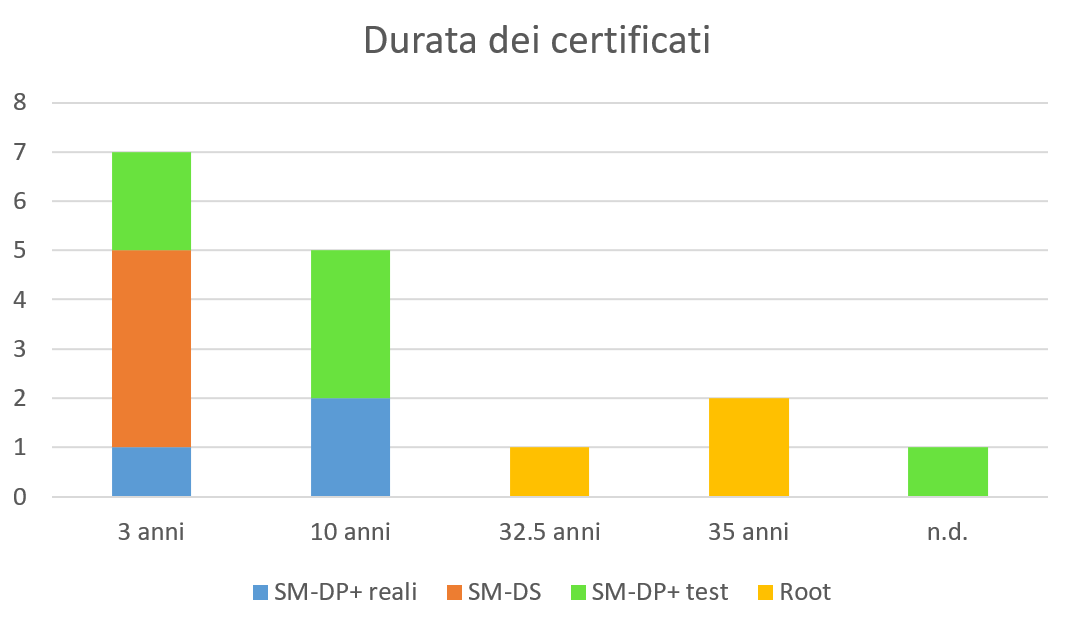
\includegraphics[width=\linewidth]{cert-duration.png}
\caption{Durata dei certificati dei server SM-DP+ e delle Root CA.}
\label{fig:cert-duration}
\end{figure}
\begin{figure}
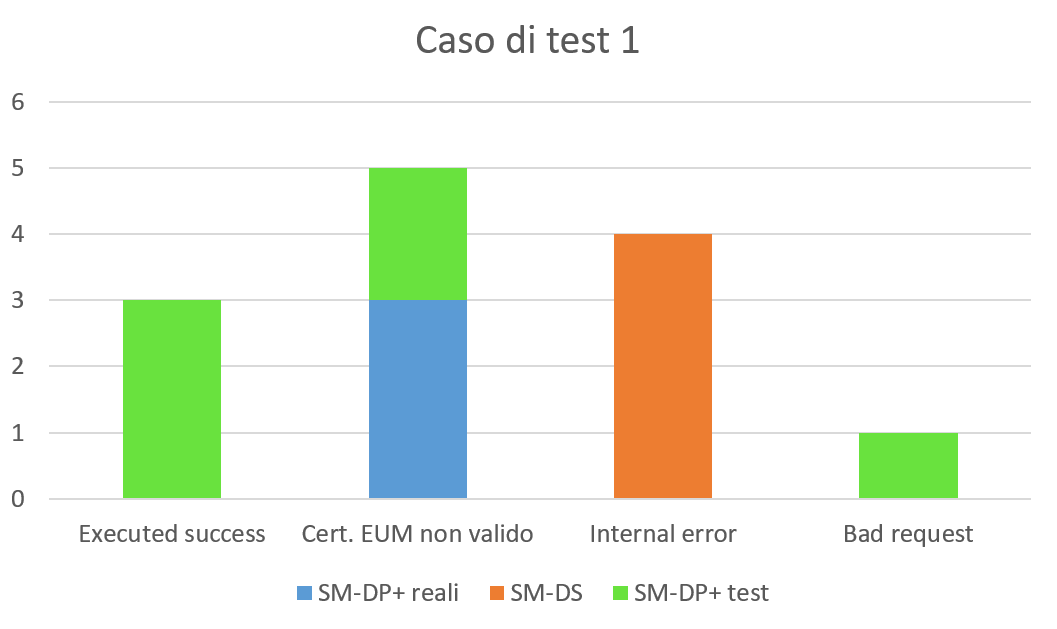
\includegraphics[width=\linewidth]{test-1.png}
\caption{Risposte dei server SM-DP+ nel caso di test 1.}
\label{fig:test-1}
\end{figure}
\begin{figure}
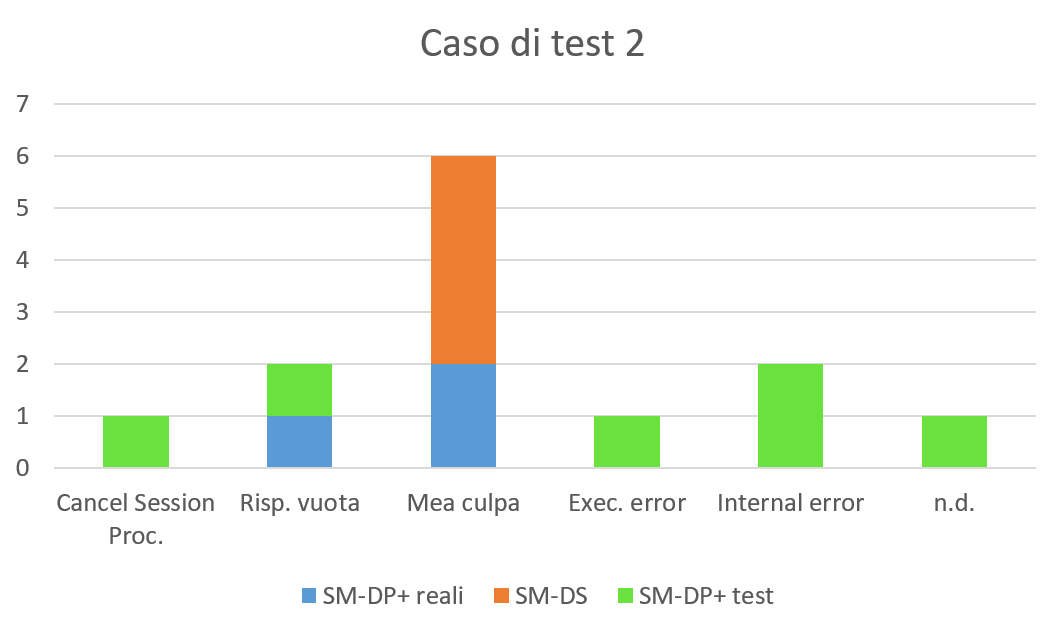
\includegraphics[width=\linewidth]{test-2.png}
\caption{Risposte dei server SM-DP+ nel caso di test 2.}
\label{fig:test-2}
\end{figure}
\begin{figure}
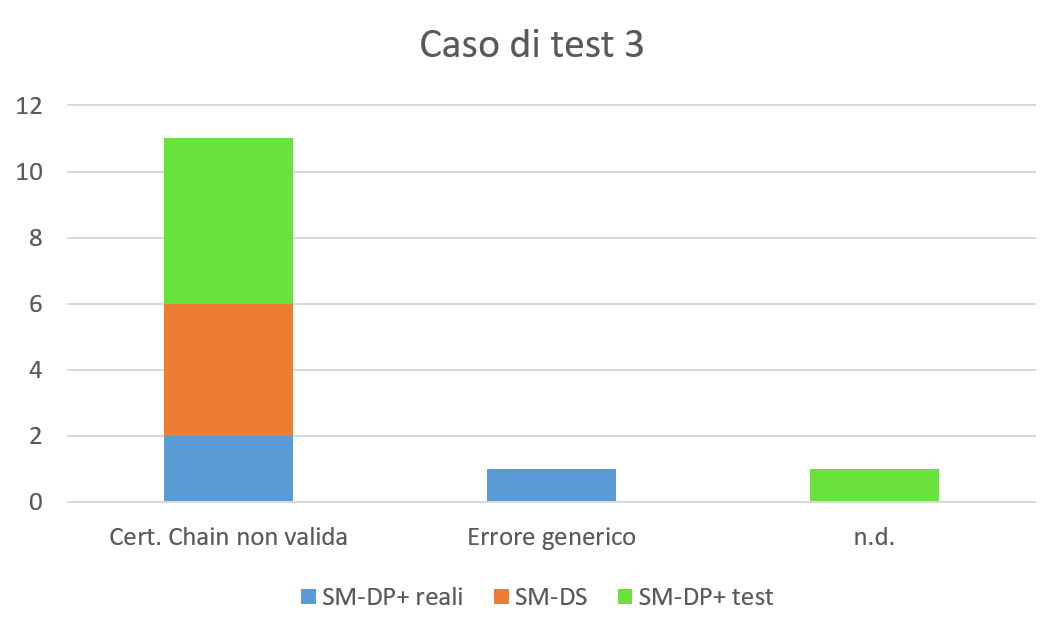
\includegraphics[width=\linewidth]{test-3.png}
\caption{Risposte dei server SM-DP+ nel caso di test 3.}
\label{fig:test-3}
\end{figure}
\begin{figure}
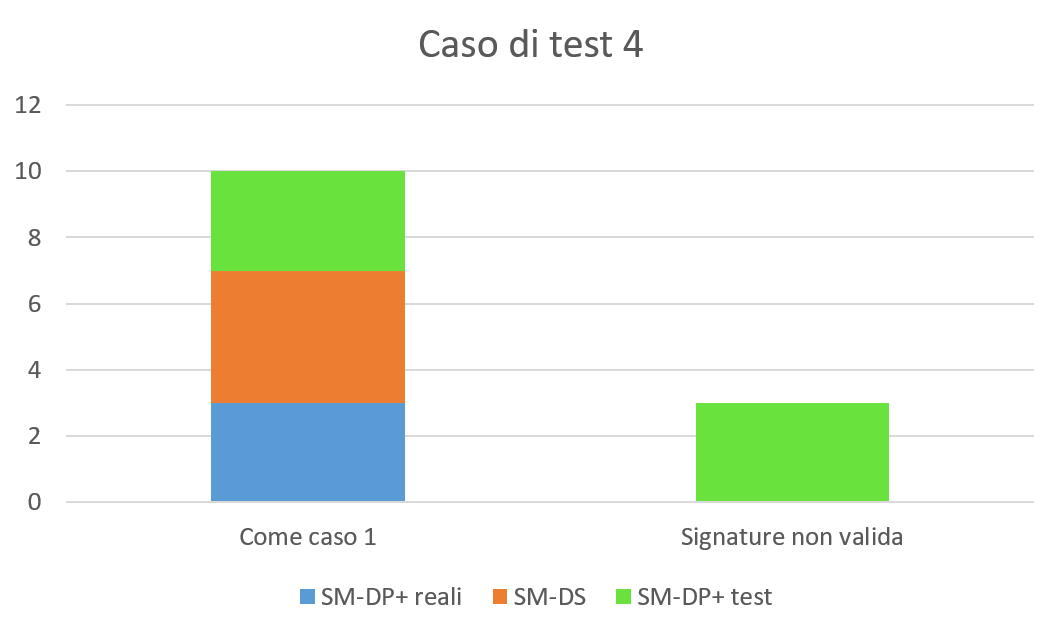
\includegraphics[width=\linewidth]{test-4.png}
\caption{Risposte dei server SM-DP+ nel caso di test 4.}
\label{fig:test-4}
\end{figure}
\begin{figure}
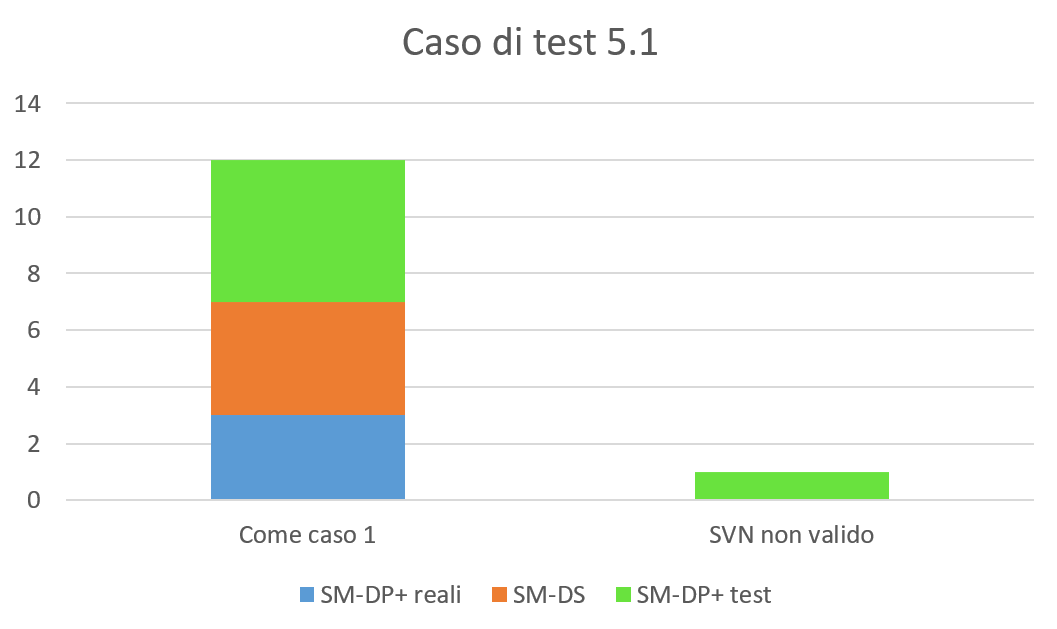
\includegraphics[width=\linewidth]{test-5-1.png}
\caption{Risposte dei server SM-DP+ nel caso di test 5.1.}
\label{fig:test-5-1}
\end{figure}
\begin{figure}
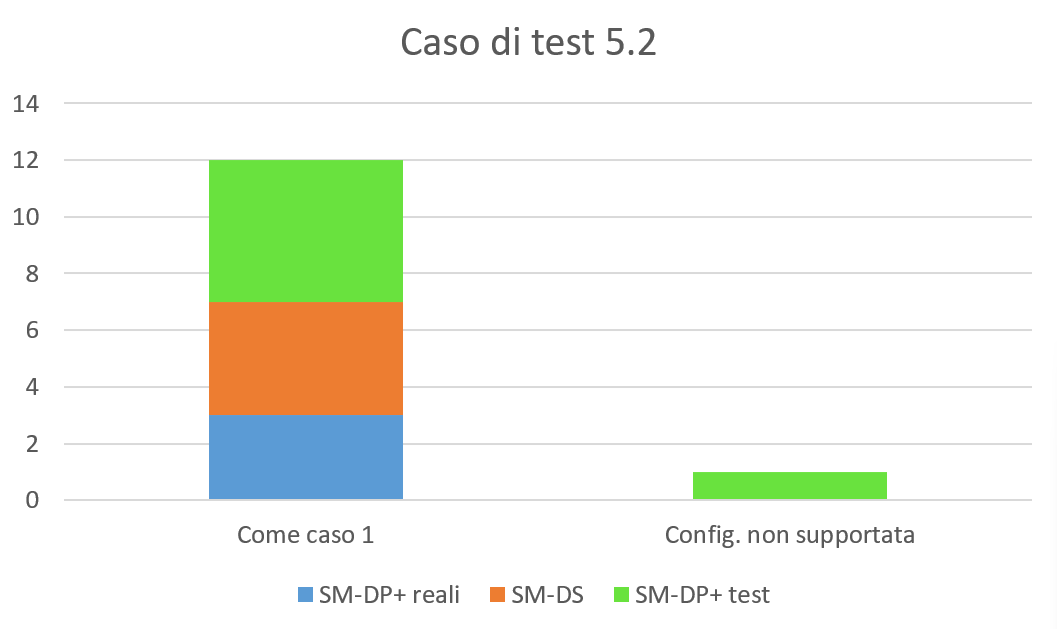
\includegraphics[width=\linewidth]{test-5-2.png}
\caption{Risposte dei server SM-DP+ nel caso di test 5.2.}
\label{fig:test-5-2}
\end{figure}
\begin{figure}
\includegraphics[width=\linewidth]{test-6-2.png}
\caption{Risposte dei server SM-DP+ nel caso di test 6.2.}
\label{fig:test-6-2}
\end{figure}
\begin{figure}
\includegraphics[width=\linewidth]{test-7-1.png}
\caption{Risposte dei server SM-DP+ nel caso di test 7.1.}
\label{fig:test-7-1}
\end{figure}
\begin{figure}
\includegraphics[width=\linewidth]{test-7-2.png}
\caption{Risposte dei server SM-DP+ nel caso di test 7.2.}
\label{fig:test-7-2}
\end{figure}
\begin{figure}
\includegraphics[width=\linewidth]{test-8.png}
\caption{Risposte dei server SM-DP+ nel caso di test 8.}
\label{fig:test-8}
\end{figure}
\begin{figure}
\includegraphics[width=\linewidth]{test-9.png}
\caption{Risposte dei server SM-DP+ nel caso di test 9.}
\label{fig:test-9}
\end{figure}
\begin{figure}
\includegraphics[width=\linewidth]{test-10.png}
\caption{Risposte dei server SM-DP+ nel caso di test 10.}
\label{fig:test-10}
\end{figure}
\begin{figure}
\includegraphics[width=\linewidth]{test-11.png}
\caption{Risposte dei server SM-DP+ nel caso di test 11.}
\label{fig:test-11}
\end{figure}
\begin{figure}
\includegraphics[width=\linewidth]{test-12-1.png}
\caption{Risposte dei server SM-DP+ nel caso di test 12.1.}
\label{fig:test-12-1}
\end{figure}
\begin{figure}
\includegraphics[width=\linewidth]{test-12-2.png}
\caption{Risposte dei server SM-DP+ nel caso di test 12.2.}
\label{fig:test-12-2}
\end{figure}
\begin{figure}
\includegraphics[width=\linewidth]{test-13-1.png}
\caption{Risposte dei server SM-DP+ nel caso di test 13.1.}
\label{fig:test-13-1}
\end{figure}
\begin{figure}
\includegraphics[width=\linewidth]{test-14-1.png}
\caption{Risposte dei server SM-DP+ nel caso di test 14.1.}
\label{fig:test-14-1}
\end{figure}

\subsection{Osservazioni sulle risposte ricevute}
Osservando i grafici riportati nel paragrafo precedente, è possibile fare le seguenti osservazioni:
\begin{itemize}
\item La maggior parte dei server SM-DP+ esaminati continua a fornire la medesima risposta del caso di test 1 anche nell'evenienza in cui viene inviata una euiccSignature1, un SVN (all'interno di euiccInfo2), un euiccCiPKIdListForVerification (all'interno di euiccInfo2), un euiccCiPKIdListForSigning (all'interno di euiccInfo2), un transactionId (all'interno di euiccSigned1), un smdpAddress (all'interno di euiccSigned1) oppure una serverChallenge (all'interno di euiccSigned1) non valida. Con ogni probabilità, ciò è indice del fatto che molti server effettuano prima un controllo sui certificati inviati dal client (eumCertificate, euiccCertificate) e solo poi sulle informazioni appena elencate. Tuttavia, è anche vero che i server di Sysmocom e Osmo-smdpp continuano a dare un esito positivo a seguito della manomissione dell'SVN, dell'euiccCiPKIdListForVerification, dell'euiccCiPKIdListForSigning, del transactionId e dell'smdpAddress: in altre parole, questo sottoinsieme di campi non viene valutato da Sysmocom e Osmo-smdpp. Ma poiché questi ultimi sono solo dei server di test, di base non vi è alcun problema. La faccenda diverrebbe più interessante se anche altri server SM-DP+ (e.g. quelli reali) fossero caratterizzati dalle stesse mancanze, seppure i campi in questione, se presi singolarmente, non sono particolarmente critici. Di fatto, SVN, euiccCiPKIdListForVerification ed euiccCiPKIdListForSigning vengono già negoziati a partire dal primo messaggio del client (initiateAuthentication) per cui all'interno di euiccInfo2, nel secondo messaggio (authenticateClient), sono dei campi ridondanti; anche l'hostname del server (smdpAddress) deve essere inviato già nel messaggio initiateAuthentication; infine, l'ID di transazione viene riportato nel messaggio authenticateClient anche esternamente alla struttura euiccSigned1, per cui è comprensibile, anche se probabilmente poco sicuro, che i server verifichino soltanto una delle due istanze dell'ID di transazione all'interno del messaggio.
\item Per ovvie ragioni, il caso di test 6.2, che consiste nell'invio di un Matching ID errato, coinvolge esclusivamente i server SM-DP+ di test, i quali sono gli unici a mettere a disposizione dei profili di test coi relativi Matching ID. L'unico server di test escluso da questa analisi è Infineon, che risponde deterministicamente con HTTP\_BAD\_REQUEST. Gli unici due server che nel caso di test 6.2 si comportano esattamente come nel caso di test 1 sono quelli di Stork \& Google e Truphone, i quali evidentemente effettuano prima il controllo sui certificati ricevuti da parte del client e solo successivamente il controllo sul Matching ID.
\item Gli unici casi in cui i server SM-DS forniscono un errore previsto dalle specifiche e non vanno in crash dando un HTTP\_INTERNAL\_SERVER\_ERROR sono:
\begin{itemize}
\item invio di uno stato di errore nel messaggio authenticateClient;
\item invio di una certificate chain diversa da quella già stabilita in euiccCiPKIdToBeUsed;
\item invio di un hostname (serverAddress) non valido nel messaggio initiateAuthentication;
\item invio di un SVN non valido nel messaggio initiateAuthentication;
\item invio di un euiccCiPKIdListForVerification o di un euiccCiPKIdListForSigning non valido nel messaggio initiateAuthentication.
\end{itemize}
Se invece i server SM-DS ricevono un messaggio inatteso, tendono a rispondere con\\ HTTP\_NOT\_FOUND. Ciò fa pensare che l'implementazione dei server SM-DS che si possono trovare in rete sia incompleta e non del tutto affidabile.
\item Se il client invia un'euiccChallenge non conforme alle specifiche (i.e. di una lunghezza diversa dai 16 byte), questa viene rifiutata solo dai server reali e da Truphone; d'altra parte, i server SM-DS, il server di Stork \& Google e il simulatore accettano anche euiccChallenge di un solo byte, lasciando eventualmente maggiore spazio di manovra ad attacchi di tipo spoofing; infine, Sysmocom e Osmo-smdpp vanno in crash se ricevono una challenge di lunghezza differente dai 16 byte.
\item Senza contare euiccChallenge, tutti i server rispondono con un opportuno messaggio di errore nel caso in cui ricevano il messaggio initiateAuthentication con almeno un campo non valido (serverAddress, SVN, euiccCiPKIdListForVerification o euiccCiPKIdListForSigning). L'unica eccezione è data dai server di test Sysmocom e Osmo-smdpp che accettano qualunque SVN, il che è comprensibile.
\item Il protocollo studiato e le relative implementazioni dei server esaminati nei vari esperimenti prevedono che, quando si verifica una condizione di errore (e.g. un end-host invia un valore errato o non valido), l'entità che riscontra tale condizione risponda con un messaggio di errore in cui, mediante il subject code e il reason code, viene specificato con esattezza cos'è andato storto. Tuttavia, inviare dei messaggi di errore così dettagliati potrebbe aprire le porte a delle vulnerabilità, poiché potenzialmente potrebbe fornire a un attaccante delle informazioni in eccesso riguardo ciò che sta avvenendo durante la comunicazione.
\end{itemize}

\section{Ottenimento dei client da testare}
La selezione dei client da testare può essere effettuata sulla base delle risorse (i.e. eUICC e dispositivi mobili) che si hanno a disposizione durante la fase di sperimentazione. In particolare, sono stati individuati i seguenti client:
\begin{itemize}
\item eUICC programmabile e LPA EasyEUICC installati manualmente in un Google Pixel 6 (mostrato in figura \ref{fig:pixel6});
\item eUICC e LPA direttamente forniti dal Google Pixel 6.
\end{itemize}
Assumendo di voler considerare anche il lettore di SIM e il simulatore del client come possibili partecipanti dei successivi esperimenti, la tabella \ref{tab:all-clients} mostra tutti i client che verranno impiegati durante l'esecuzione dei test.

\begin{table}[h!]
\begin{center}
\captionsetup{skip=4pt}
\caption{Elenco dei client coinvolti negli esperimenti.}
\label{tab:all-clients}
\begin{tabularx}{\textwidth}{|c|X|X|} % <-- Alignments: 1nd column center, with vertical lines in between
\hline
\textbf{Nome} & \textbf{Descrizione} & \textbf{Note}\\
\hline
Google Pixel 6 & Client reale & Utilizzerà una certificate chain di test.\\
\hline
EasyEUICC & eUICC programmabile + LPA EasyEUICC & Utilizzerà una certificate chain di test.\\
\hline
LPAC & eUICC programmabile + lpac & Utilizzerà una certificate chain di test.\\
\hline
Simulatore & Simulatore lato client precedentemente implementato & Utilizzerà una certificate chain di test.\\
\hline
\end{tabularx}
\end{center}
\end{table}

\section{Risposte dei client testati}
\subsection{Casi di test definiti}
I casi di test che sono stati implementati per valutare l'interazione tra il simulatore del server e i client a disposizione sono riportati nella tabella \ref{tab:clients-test-cases}.\\
\begin{table}[h!]
\begin{center}
\captionsetup{skip=4pt}
\caption{Elenco dei casi di test definiti per i client a disposizione.}
\label{tab:clients-test-cases}
\begin{tabularx}{\textwidth}{|c|X|} % <-- Alignments: 1st column center, with vertical lines in between
\hline
\textbf{ID} & \textbf{Descrizione}\\
\hline
1 & Il simulatore del server si comporta perfettamente come da specifiche.\\
\hline
2 & Manomissione del messaggio getBoundProfilePackageResponse: invio di un profilo dummy non crittografato.\\
\hline
3.1 & Manomissione del messaggio getBoundProfilePackageResponse: utilizzo di un Transaction ID non valido all'interno del sotto-campo initialiseSecureChannelRequest.\\
\hline
3.2 & Manomissione del messaggio getBoundProfilePackageResponse: utilizzo di una chiave pubblica one-time smdpOtpk casuale e non generata tramite ECDSA all'interno del sotto-campo initialiseSecureChannelRequest.\\
\hline
3.3 & Manomissione del messaggio getBoundProfilePackageResponse: calcolo errato della signature (smdpSign) all'interno del sotto-campo initialiseSecureChannelRequest.\\
\hline
4.1 & Manomissione del messaggio authenticateClientResponse: utilizzo di un iccid casuale all'interno del campo profileMetadata.\\
\hline
4.2 & Manomissione del messaggio authenticateClientResponse: eliminazione di profileClass, notificationConfigurationInfo e profileOwner dal campo profileMetadata.\\
\hline
4.3 & Manomissione del messaggio authenticateClientResponse: inserimento delle Profile Policy Rules all'interno del campo profileMetadata.\\
\hline
5 & Manomissione del messaggio authenticateClientResponse: ccRequiredFlag = True all'interno del campo smdpSigned2.\\
\hline
6.1 & Manomissione del messaggio authenticateClientResponse: utilizzo di un Transaction ID non valido all'interno del campo smdpSigned2.\\
\hline
6.2 & Manomissione del messaggio authenticateClientResponse: campo transactionId non valido direttamente all'interno del messaggio.\\
\hline
7 & Manomissione del messaggio authenticateClientResponse:  calcolo errato dalla signature (smdpSignature2).\\
\hline
8 & Manomissione del messaggio authenticateClientResponse: invio di un certificato smdpCertificate diverso da quello previsto.\\
\hline
9.1 & Manomissione del messaggio initiateAuthenticationResponse: utilizzo di una euiccChallenge non valida all'interno del campo serverSigned1.\\
\hline
9.2 & Manomissione del messaggio initiateAuthenticationResponse: utilizzo di una serverChallenge malforme (e.g. 0x00) all'interno del campo serverSigned1.\\
\hline
9.3 & Manomissione del messaggio initiateAuthenticationResponse: utilizzo di un serverAddress non corrispondente all'hostname realmente assegnato al simulatore del server.\\
\hline
10.1 & Manomissione del messaggio initiateAuthenticationResponse: utilizzo di Transaction ID differenti all'interno del campo serverSigned1 e direttamente nel messaggio.\\
\hline
10.2 & Manomissione del messaggio initiateAuthenticationResponse: utilizzo di un Transaction ID malforme direttamente all'interno del messaggio (e.g. 0x00).\\
\hline
11 & Manomissione del messaggio initiateAuthenticationResponse: calcolo errato dalla signature (serverSignature1).\\
\hline
12 & Manomissione del messaggio initiateAuthenticationResponse: invio di un certificato serverCertificate diverso da quello previsto.\\
\hline
13 & Manomissione del messaggio initiateAuthenticationResponse: invio di una certificate chain identificata da euiccCiPKIdToBeUsed che non rientra in euiccCiPKIdListForVerification o euiccCiPKIdListForSigning.\\
\hline
14.1 & Invio di getBoundProfilePackageResponse come primo messaggio.\\
\hline
14.2 & Invio di getBoundProfilePackageResponse come secondo messaggio.\\
\hline
\end{tabularx}
\end{center}
\end{table}

\begin{figure}
\includegraphics[width=\linewidth]{pixel6.png}
\caption{Il Google Pixel 6 coinvolto negli esperimenti.}
\label{fig:pixel6}
\end{figure}

\subsubsection{Caso di test 1}
Consiste nel comunicare col client (in particolare con l'LPA) seguendo fedelmente le specifiche, senza alcuna manomissione nel protocollo o nei messaggi inviati. Di seguito è descritto il comportamento dei client in esame in questo caso di test.
\begin{itemize}
\item \textbf{Google Pixel 6}: impossibile connettersi alla rete: non viene inviato nemmeno il messaggio initiateAuthentication. Ciò potrebbe essere dovuto al fatto che il client in questione non supporta i server SM-DP+ di test.
\item \textbf{EasyEUICC}: \textit{errorResult} al quarto messaggio di richiesta (pendingNotification), con\\ \textit{scp03tSecurityError}, che corrisponde all'errore riscontrato e non risolto durante la fase di validazione.
\item \textbf{LPAC}: errore dopo il terzo messaggio di risposta (getBoundProfilePackageResponse), con \textit{scp03t\_security\_error}, che è esattamente l'errore riscontrato e non risolto durante la fase di validazione.
\item \textbf{Simulatore}: il profilo viene installato con successo.
\end{itemize}

\subsubsection{Caso di test 2}
Consiste nel manomettere il messaggio getBoundProfilePackageResponse inserendo all'interno dei sotto-campi firstSequenceOf87, sequenceOf88, secondSequenceOf87 e sequenceOf86 dei byte casuali (e.g. tutti pari a 0x00), in modo tale da rappresentare dei metadati e un profilo dummy non crittografato.
\begin{itemize}
\item \textbf{Google Pixel 6}: n.d.
\item \textbf{EasyEUICC}: \textit{errorResult} al quarto messaggio di richiesta (pendingNotification), con\\ \textit{scp03tSecurityError}.
\item \textbf{LPAC}: errore dopo il terzo messaggio di risposta (getBoundProfilePackageResponse), con \textit{scp03t\_security\_error}.
\item \textbf{Simulatore}: Common Cancel Session Procedure completata con successo a seguito del terzo messaggio di risposta da parte del server (getBoundProfilePackageResponse).
\end{itemize}

\subsubsection{Caso di test 3.1}
Consiste nel manomettere il messaggio getBoundProfilePackageResponse ponendo il Transaction ID all'interno del sotto-campo initialiseSecureChannelRequest pari a un valore non valido.
\begin{itemize}
\item \textbf{Google Pixel 6}: n.d.
\item \textbf{EasyEUICC}: \textit{errorResult} al quarto messaggio di richiesta (pendingNotification), con\\ \textit{invalidTransactionId}.
\item \textbf{LPAC}: errore dopo il terzo messaggio di risposta (getBoundProfilePackageResponse), con \textit{invalid\_transaction\_id}.
\item \textbf{Simulatore}: \textit{errorResult} al quarto messaggio di richiesta (pendingNotification), con\\ \textit{invalidTransactionId}.
\end{itemize}

\subsubsection{Caso di test 3.2}
Consiste nel manomettere il messaggio getBoundProfilePackageResponse inserendo all'interno del sotto-campo initialiseSecureChannelRequest una chiave pubblica one-time smdpOtpk non generata tramite ECDSA, bensì espressa sottoforma di byte casuali.
\begin{itemize}
\item \textbf{Google Pixel 6}: n.d.
\item \textbf{EasyEUICC}: interruzione della comunicazione dopo il terzo messaggio di risposta (getBoundProfilePackageResponse).
\item \textbf{LPAC}: errore dopo il terzo messaggio di risposta (getBoundProfilePackageResponse), con \textit{unknown}.
\item \textbf{Simulatore}: il profilo viene installato con successo.
\end{itemize}

\subsubsection{Caso di test 3.3}
Consiste nel manomettere il messaggio getBoundProfilePackageResponse ponendo il campo smdpSign pari a un valore diverso dalla signature ottenuta firmando tutte le altre entry del sotto-campo initialiseSecureChannelRequest con la chiave privata del server SM-DP+.
\begin{itemize}
\item \textbf{Google Pixel 6}: n.d.
\item \textbf{EasyEUICC}: \textit{errorResult} al quarto messaggio di richiesta (pendingNotification), con\\ \textit{invalidSignature}.
\item \textbf{LPAC}: errore dopo il terzo messaggio di risposta (getBoundProfilePackageResponse), con \textit{invalid\_signature}.
\item \textbf{Simulatore}: \textit{errorResult} al quarto messaggio di richiesta (pendingNotification), con\\ \textit{invalidSignature}.
\end{itemize}

\subsubsection{Caso di test 4.1}
Consiste nel manomettere il messaggio authenticateClientResponse inserendo all'interno del campo profileMetadata un iccid casuale e non quello originariamente assegnato al profilo che il client vuole scaricare.
\begin{itemize}
\item \textbf{Google Pixel 6}: n.d.
\item \textbf{EasyEUICC}: \textit{errorResult} al quarto messaggio di richiesta (pendingNotification), con\\ \textit{scp03tSecurityError}.
\item \textbf{LPAC}: errore dopo il terzo messaggio di risposta (getBoundProfilePackageResponse), con \textit{scp03t\_security\_error}.
\item \textbf{Simulatore}: il profilo viene installato con successo.
\end{itemize}

\subsubsection{Caso di test 4.2}
Consiste nel manomettere il messaggio authenticateClientResponse eliminando le entry relative a profileClass, notificationConfigurationInfo e profileOwner dal campo profileMetadata. Trattandosi solo di informazioni opzionali, questo caso di test non dovrebbe produrre un risultato differente dal caso di test 1.
\begin{itemize}
\item \textbf{Google Pixel 6}: n.d.
\item \textbf{EasyEUICC}: \textit{errorResult} al quarto messaggio di richiesta (pendingNotification), con\\ \textit{scp03tSecurityError}.
\item \textbf{LPAC}: errore dopo il terzo messaggio di risposta (getBoundProfilePackageResponse), con \textit{scp03t\_security\_error}.
\item \textbf{Simulatore}: il profilo viene installato con successo.
\end{itemize}

\subsubsection{Caso di test 4.3}
Consiste nel manomettere il messaggio authenticateClientResponse aggiungendo una entry relativa alle Profile Policy Rules all'interno del campo profileMetadata. In particolare, tale entry indica l'attivazione di entrambe le Profile Policy Rules (PPR1, PPR2).
\begin{itemize}
\item \textbf{Google Pixel 6}: n.d.
\item \textbf{EasyEUICC}: \textit{errorResult} al quarto messaggio di richiesta (pendingNotification), con\\ \textit{scp03tSecurityError}.
\item \textbf{LPAC}: errore dopo il terzo messaggio di risposta (getBoundProfilePackageResponse), con \textit{scp03t\_security\_error}.
\item \textbf{Simulatore}: il profilo viene installato con successo dopo una conferma all'utente sulla sottoscrizione delle PPR.
\end{itemize}

\subsubsection{Caso di test 5}
Consiste nel manomettere il messaggio authenticateClientResponse ponendo ccRequiredFlag all'interno del campo smdpSigned2 pari a True, in modo tale da richiedere al client l'immissione di un Confirmation Code.
\begin{itemize}
\item \textbf{Google Pixel 6}: n.d.
\item \textbf{EasyEUICC}:
\begin{itemize}
\item Caso in cui l'utente ha immesso un qualunque Confirmation Code $\rightarrow$ \textit{errorResult} al quarto messaggio di richiesta (pendingNotification), con \textit{scp03tSecurityError}.
\item Caso in cui l'utente non ha immesso alcun Confirmation Code $\rightarrow$ \textit{prepareDownloadResponseError} al terzo messaggio di richiesta (getBoundProfilePackage), con \textit{undefinedError}.
\end{itemize}
\item \textbf{LPAC}:
\begin{itemize}
\item Caso in cui l'utente ha immesso un qualunque Confirmation Code $\rightarrow$ errore dopo il terzo messaggio di risposta (getBoundProfilePackageResponse), con \textit{scp03t\_security\_error}.
\item Caso in cui l'utente non ha immesso alcun Confirmation Code $\rightarrow$ errore generico dopo il secondo messaggio di risposta (authenticateClientResponse).
\end{itemize}
\item \textbf{Simulatore}:
\begin{itemize}
\item Caso in cui l'utente ha immesso un qualunque Confirmation Code $\rightarrow$ il profilo viene installato con successo.
\item Caso in cui l'utente non ha immesso alcun Confirmation Code $\rightarrow$ Common Cancel Session Procedure completata con successo a seguito del secondo messaggio di risposta da parte del server (authenticateClientResponse).
\end{itemize}
\end{itemize}

\subsubsection{Caso di test 6.1}
Consiste nel manomettere il messaggio authenticateClientResponse ponendo il Transaction ID all'interno del campo smdpSigned2 pari a un valore non valido.
\begin{itemize}
\item \textbf{Google Pixel 6}: n.d.
\item \textbf{EasyEUICC}: \textit{prepareDownloadResponseError} al terzo messaggio di richiesta (getBoundProfilePackage), con \textit{invalidTransactionId}.
\item \textbf{LPAC}: \textit{prepareDownloadResponseError} al terzo messaggio di richiesta (getBoundProfilePackage), con \textit{invalidTransactionId}.
\item \textbf{Simulatore}: \textit{prepareDownloadResponseError} al terzo messaggio di richiesta (getBoundProfilePackage), con \textit{invalidTransactionId}.
\end{itemize}

\subsubsection{Caso di test 6.2}
Consiste nel manomettere il messaggio authenticateClientResponse ponendo il Transaction ID pari a un valore non valido direttamente all’interno messaggio stesso.
\begin{itemize}
\item \textbf{Google Pixel 6}: n.d.
\item \textbf{EasyEUICC}: \textit{errorResult} al quarto messaggio di richiesta (pendingNotification), con\\ \textit{scp03tSecurityError}.
\item \textbf{LPAC}: errore dopo il terzo messaggio di risposta (getBoundProfilePackageResponse), con \textit{scp03t\_security\_error}.
\item \textbf{Simulatore}: \textit{prepareDownloadResponseError} al terzo messaggio di richiesta (getBoundProfilePackage), con \textit{invalidTransactionId}.
\end{itemize}

\subsubsection{Caso di test 7}
Consiste nel manomettere il messaggio authenticateClientResponse ponendo il campo smdpSignature2 pari a un valore diverso dalla signature ottenuta firmando smdpSigned2+euiccSignature1 con la chiave privata del server SM-DP+.
\begin{itemize}
\item \textbf{Google Pixel 6}: n.d.
\item \textbf{EasyEUICC}: \textit{prepareDownloadResponseError} al terzo messaggio di richiesta (getBoundProfilePackage), con \textit{undefinedError}.
\item \textbf{LPAC}: errore generico dopo il secondo messaggio di risposta (authenticateClientResponse).
\item \textbf{Simulatore}: \textit{prepareDownloadResponseError} al terzo messaggio di richiesta (getBoundProfilePackage), con \textit{invalidSignature}.
\end{itemize}

\subsubsection{Caso di test 8}
Consiste nel manomettere il messaggio authenticateClientResponse inserendo all’interno del campo smdpCertificate un certificato appartenente a una certificate chain differente da quella dichiarata precedentemente in euiccCiPKIdToBeUsed.
\begin{itemize}
\item \textbf{Google Pixel 6}: n.d.
\item \textbf{EasyEUICC}: \textit{prepareDownloadResponseError} al terzo messaggio di richiesta (getBoundProfilePackage), con \textit{invalidCertificate}.
\item \textbf{LPAC}: \textit{prepareDownloadResponseError} al terzo messaggio di richiesta (getBoundProfilePackage), con \textit{invalidCertificate}.
\item \textbf{Simulatore}: \textit{prepareDownloadResponseError} al terzo messaggio di richiesta (getBoundProfilePackage), con \textit{invalidCertificate}.
\end{itemize}

\subsubsection{Caso di test 9.1}
Consiste nel manomettere il messaggio initiateAuthenticationResponse ponendo il sotto-campo euiccChallenge del campo serverSigned1 pari a un valore che non corrisponde alla challenge inviata dal client nel messaggio precedente (initiateAuthentication).
\begin{itemize}
\item \textbf{Google Pixel 6}: n.d.
\item \textbf{EasyEUICC}: \textit{authenticateResponseError} al secondo messaggio di richiesta (authenticateClient), con \textit{euiccChallengeMismatch}.
\item \textbf{LPAC}: \textit{authenticateResponseError} al secondo messaggio di richiesta (authenticateClient), con \textit{euiccChallengeMismatch}.
\item \textbf{Simulatore}: \textit{authenticateResponseError} al secondo messaggio di richiesta (authenticateClient), con \textit{euiccChallengeMismatch}.
\end{itemize}

\subsubsection{Caso di test 9.2}
Consiste nel manomettere il messaggio initiateAuthenticationResponse utilizzando una serverChallenge malforme (e.g. 0x00, che ha una lunghezza differente dai 16 byte di default, e comunque troppo ridotta per svolgere il ruolo di challenge).
\begin{itemize}
\item \textbf{Google Pixel 6}: n.d.
\item \textbf{EasyEUICC}: interruzione della comunicazione dopo il primo messaggio di risposta (initiateAuthenticationResponse).
\item \textbf{LPAC}: errore generico dopo il primo messaggio di risposta (initiateAuthenticationResponse).
\item \textbf{Simulatore}: il profilo viene installato con successo.
\end{itemize}

\subsubsection{Caso di test 9.3}
Consiste nel manomettere il messaggio initiateAuthenticationResponse ponendo il sotto-campo serverAddress del campo serverSigned1 pari a una stringa che non corrisponde all’effettivo hostname del simulatore del server.
\begin{itemize}
\item \textbf{Google Pixel 6}: n.d.
\item \textbf{EasyEUICC}: invio del serverAddress errato nel secondo messaggio di richiesta (authenticateClient).
\item \textbf{LPAC}: invio del serverAddress errato nel secondo messaggio di richiesta (authenticateClient).
\item \textbf{Simulatore}: \textit{authenticateResponseError} al secondo messaggio di richiesta (authenticateClient), con \textit{invalidOid}.
\end{itemize}

\subsubsection{Caso di test 10.1}
Consiste nel manomettere il messaggio initiateAuthenticationResponse ponendo il Transaction ID all'interno del campo serverSigned1 pari a un valore differente dal Transaction ID situato direttamente all'interno del messaggio stesso.
\begin{itemize}
\item \textbf{Google Pixel 6}: n.d.
\item \textbf{EasyEUICC}: invio del Transaction ID errato nel secondo messaggio di richiesta (authenticateClient).
\item \textbf{LPAC}: invio del Transaction ID errato nel secondo messaggio di richiesta (authenticateClient).
\item \textbf{Simulatore}: \textit{authenticateResponseError} al secondo messaggio di richiesta (authenticateClient), con \textit{undefinedError}.
\end{itemize}

\subsubsection{Caso di test 10.2}
Consiste nel manomettere il messaggio initiateAuthenticationResponse utilizzando un Transaction ID malforme (e.g. 0x00, che ha una lunghezza differente dai 16 byte di default, e comunque troppo ridotta per svolgere il ruolo di challenge).
\begin{itemize}
\item \textbf{Google Pixel 6}: n.d.
\item \textbf{EasyEUICC}: \textit{errorResult} al quarto messaggio di richiesta (pendingNotification), con\\ \textit{scp03tSecurityError}.
\item \textbf{LPAC}: errore dopo il terzo messaggio di risposta (getBoundProfilePackageResponse), con \textit{scp03t\_security\_error}.
\item \textbf{Simulatore}: il profilo viene installato con successo.
\end{itemize}

\subsubsection{Caso di test 11}
Consiste nel manomettere il messaggio initiateAuthenticationResponse ponendo il campo serverSignature1 pari a un valore diverso dalla signature ottenuta firmando serverSigned1 con la chiave privata del server SM-DP+.
\begin{itemize}
\item \textbf{Google Pixel 6}: n.d.
\item \textbf{EasyEUICC}: \textit{authenticateResponseError} al secondo messaggio di richiesta (authenticateClient), con \textit{undefinedError}.
\item \textbf{LPAC}: errore generico dopo il primo messaggio di risposta (initiateAuthenticationResponse).
\item \textbf{Simulatore}: \textit{authenticateResponseError} al secondo messaggio di richiesta (authenticateClient), con \textit{invalidSignature}.
\end{itemize}

\subsubsection{Caso di test 12}
Consiste nel manomettere il messaggio initiateAuthenticationResponse inserendo all’interno del campo serverCertificate un certificato appartenente a una certificate chain differente da quella dichiarata in euiccCiPKIdToBeUsed.
\begin{itemize}
\item \textbf{Google Pixel 6}: n.d.
\item \textbf{EasyEUICC}: \textit{authenticateResponseError} al secondo messaggio di richiesta (authenticateClient), con \textit{invalidOid}.
\item \textbf{LPAC}: \textit{authenticateResponseError} al secondo messaggio di richiesta (authenticateClient), con \textit{invalidOid}.
\item \textbf{Simulatore}: \textit{authenticateResponseError} al secondo messaggio di richiesta (authenticateClient), con \textit{invalidCertificate}.
\end{itemize}

\subsubsection{Caso di test 13}
Consiste nel manomettere il messaggio initiateAuthenticationResponse ponendo il campo euiccCiPKIdToBeUsed pari a un valore che non rientra né in euiccCiPKIdListForVerification né in euiccCiPKIdListForSigning, in modo tale che venga indicata una certificate chain non inclusa tra quelle supportate dal client.
\begin{itemize}
\item \textbf{Google Pixel 6}: n.d.
\item \textbf{EasyEUICC}: \textit{authenticateResponseError} al secondo messaggio di richiesta (authenticateClient), con \textit{ciPKUnknown}.
\item \textbf{LPAC}: \textit{authenticateResponseError} al secondo messaggio di richiesta (authenticateClient), con \textit{ciPKUnknown}.
\item \textbf{Simulatore}: \textit{authenticateResponseError} al secondo messaggio di richiesta (authenticateClient), con \textit{ciPKUnknown}.
\end{itemize}

\subsubsection{Caso di test 14.1}
Consiste nell’inviare al client getBoundProfilePackageResponse come primo messaggio di risposta.
\begin{itemize}
\item \textbf{Google Pixel 6}: n.d.
\item \textbf{EasyEUICC}: interruzione della comunicazione dopo il messaggio di risposta getBoundProfilePackageResponse.
\item \textbf{LPAC}: errore dopo il messaggio di risposta getBoundProfilePackageResponse, con \textit{unknown}.
\item \textbf{Simulatore}: interruzione della comunicazione dopo il messaggio di risposta getBoundProfilePackageResponse.
\end{itemize}

\subsubsection{Caso di test 14.2}
Consiste nell’inviare al client getBoundProfilePackageResponse subito dopo aver ricevuto il messaggio di authenticateClient, saltando così il messaggio di authenticateClientResponse.
\begin{itemize}
\item \textbf{Google Pixel 6}: n.d.
\item \textbf{EasyEUICC}: interruzione della comunicazione dopo il messaggio di risposta getBoundProfilePackageResponse.
\item \textbf{LPAC}: errore dopo il messaggio di risposta getBoundProfilePackageResponse, con \textit{unknown}.
\item \textbf{Simulatore}: interruzione della comunicazione dopo il messaggio di risposta getBoundProfilePackageResponse.
\end{itemize}

\subsection{Certificati esibiti dai client}
Anche contestualmente all'analisi delle risposte dei client può tornare utile analizzare i certificati esibiti dai client stessi e, in particolare, CERT.EUICC.SIG (proprio dell'eUICC) e CERT.EUM.SIG (proprio dell'EUM). Tali certificati possono essere ispezionati solo per i client che hanno inviato con successo il messaggio di richiesta authenticateClient in almeno uno dei casi di test sopra citati. È perciò esclusa da questa trattazione la coppia (eUICC originale, LPA originale) del Google Pixel 6. Di seguito sono riportati i principali campi dei certificati degli altri tre client, a partire dai CERT.EUICC.SIG; poiché i client EasyEUICC e LPAC condividono la medesima eUICC, devono necessariamente aver esposto lo stesso certificato.

\subsubsection{Certificato di EasyEUICC e LPAC}
\begin{itemize}
\item \textbf{Algorithm}: ecdsaWithSHA256;
\item \textbf{issuer countryName}: ES;
\item \textbf{issuer organizationName}: RSP TEST EUM;
\item \textbf{issuer commonName}: EUM Test;
\item \textbf{validity notBefore}: 2024-01-25;
\item \textbf{validity notAfter}: 7499-11-18;
\item \textbf{countryName}: DE;
\item \textbf{organizationName}: sysmocom RSP Test EUM;
\item \textbf{commonName}: sysmoEUICC-C2T Test eUICC.
\end{itemize}

\subsubsection{Certificato del simulatore del client}
\begin{itemize}
\item \textbf{Algorithm}: ecdsaWithSHA256;
\item \textbf{issuer countryName}: ES;
\item \textbf{issuer organizationName}: RSP TEST EUM;
\item \textbf{issuer commonName}: EUM Test;
\item \textbf{validity notBefore}: 2020-04-01;
\item \textbf{validity notAfter}: 7496-01-24;
\item \textbf{countryName}: ES;
\item \textbf{organizationName}: RSP Test EUM;
\item \textbf{commonName}: Test eUICC.
\end{itemize}

\noindent Naturalmente, sarebbe stato anche possibile far comunicare il simulatore del server col simulatore del client utilizzando la medesima certificate chain custom introdotta durante la fase degli esperimenti sui server SM-DP+ reali: non avrebbe fatto differenza.\\
Inoltre, dai campi \textit{issuer countryName}, \textit{issuer organizationName} e \textit{issuer commonName}, è possibile constatare che EasyEUICC e LPAC e, per costruzione, il simulatore del client condividono il medesimo EUM, il cui certificato CERT.EUM.SIG è descritto qui di seguito.

\subsubsection{Certificato dell'EUM}
\begin{itemize}
\item \textbf{Algorithm}: ecdsaWithSHA256;
\item \textbf{issuer countryName}: IT;
\item \textbf{issuer organizationName}: RSPTEST;
\item \textbf{issuer organizationalUnitName}: TESTCERT;
\item \textbf{issuer commonName}: Test CI;
\item \textbf{validity notBefore}: 2020-04-01;
\item \textbf{validity notAfter}: 2054-03-24;
\item \textbf{countryName}: ES;
\item \textbf{organizationName}: RSP Test EUM;
\item \textbf{commonName}: EUM Test;
\item \textbf{crLDistributionPoints}: http://ci.test.example.com/crl-B.crl;
\item \textbf{authorityKeyIdentifier}: sgp.
\end{itemize}

\subsection{Analisi delle risposte ricevute}
Per quanto concerne l'eUICC e l'applicazione LPA integrati nel Google Pixel 6, si potrebbe provare a capire quali siano le ragioni per cui la connessione non va a buon fine. È stato dunque catturato il traffico di rete nella comunicazione tra il dispositivo mobile e il simulatore del server ed è stato analizzato con Wireshark, come testimoniato dalla figura \ref{fig:wireshark-pixel}.
\begin{figure}
\includegraphics[width=\linewidth]{wireshark-pixel.png}
\caption{Cattura Wireshark della comunicazione tra il Google Pixel 6 e il simulatore del server.}
\label{fig:wireshark-pixel}
\end{figure}
Com'è possibile vedere, avviene l'intera procedura di handshake di TLS e, dopodiché, nel pacchetto evidenziato in blu nella figura, il dispositivo mobile invia un messaggio di [FIN, ACK] per interrompere la connessione TLS: qualcosa è andato storto durante l'handshake, come una configurazione non supportata da una delle due controparti. In particolare, sembra che il Google Pixel 6 abbia i certificati TLS caratterizzati dai PIN, grazie ai quali il dispositivo mobile è in grado di connettersi esclusivamente agli host che detengono certificati TLS specifici, e non con gli host che ne possiedono uno valido ma non previsto dai PIN.\\
Dalla figura \ref{fig:wireshark-pixel} emerge anche che la versione di TLS che stava per essere utilizzata è la 1.2: una versione ancora accettata dalla GSM Association ma non la migliore possibile. È molto probabile che la maggioranza delle comunicazioni basate sul protocollo SM-DP+ si appoggino tuttora sulla versione 1.2 di TLS.\\

\noindent Passando invece ai client sui quali è stato possibile testare il protocollo SM-DP+, balza subito all'occhio la perfetta analogia fra le risposte fornite da EasyEUICC nei vari esperimenti e quelle fornite da LPAC. Ciò era assolutamente prevedibile, dal momento in cui i due client fanno uso della medesima eUICC programmabile e differiscono soltanto dall'applicazione LPA. Si hanno dunque solo due client significativi dal punto di vista delle risposte ricevute, di cui uno è identificabile o con EasyEUICC o con LPAC, mentre l'altro è il simulatore del client sviluppato nel presente lavoro, per cui non è neanche un client in commercio. Conseguentemente, non ha molto senso graficare il comportamento dei client nei vari esperimenti come è stato fatto per i server SM-DP+; piuttosto, possono essere direttamente fatte delle osservazioni.
\begin{itemize}
\item All'interno del messaggio di risposta authenticateClientResponse si hanno due istanze di Transaction ID: una interna alla struttura smdpSigned2 e una esterna. Dai casi di test 6.1 e 6.2 emerge che EasyEUICC e LPAC controllano la correttezza soltanto dell'ID di transazione situato in smdpSigned2. Si tratta di una situazione perfettamente analoga a quella riscontrata durante l'esecuzione dei test dei server: anche nei messaggi di richiesta dei client si ha il Transaction ID ripetuto due volte e anche i server SM-DP+ verificano la correttezza del valore di una sola istanza dell'ID di transazione.
\item Anche all'interno del messaggio di risposta initiateAuthenticationResponse si hanno due istanze di Transaction ID: una interna alla struttura serverSigned1 e una esterna. Dal caso di test 10.1 si ha di nuovo che, dal punto di vista di EasyEUICC e LPAC, fa fede esclusivamente l'ID di transazione interno. Infatti, nel caso di test 10.1 il valore dei due ID è differente e i client acquisiscono quello situato in serverSigned1.
\item Nel caso di test 10.2, il Transaction ID proposto dal simulatore del server è composto da un unico byte e viene accettato così com'è dai client testati. Tuttavia, trattandosi di un nonce, sarebbe stato ideale forzare l'ID di transazione ad avere una certa entropia minima (i.e. una certa dimensione minima), in modo tale da evitare il più possibile il riuso del medesimo ID in più connessioni successive.
\item All'interno del messaggio initiateAuthenticationResponse viene specificato l'hostname del server SM-DP+ che sta inviando tale messaggio. Sulla base del caso di test 9.3, sembra succedere ciò che viene descritto qui di seguito. Il client contatta il server SM-DP+ specificando nel messaggio initiateAuthentication l'hostname effettivo del server mediante il campo smdpAddress; il server risponde specificando nel messaggio initiateAuthenticationResponse un hostname differente; a quel punto, il client si convince che l'hostname corretto del server sia quello riportato in initiateAuthenticationResponse. Tale fenomeno può essere giustificato dal fatto che ciasucn server può avere più hostname (alias). Tuttavia, cià potrebbe far sospettare che l'hostname del server potrebbe essere spoofato all'interno del messaggio initiateAuthenticationResponse.
\item Le condizioni di errore legate al calcolo errato della signature sono le uniche che vengono elaborate di EasyEUICC e LPAC come errori generici (o \textit{undefined}). In tutti gli altri casi, i client specificano sempre i dettagli sull'errore riscontrato. Si tratta nuovamente di un comportamento che è stato già osservato durante i test dei server SM-DP+.
\end{itemize}
Comunque sia, nel complesso, nonostante siano stati esaminati perlopiù client di test, il loro comportamento osservato rispecchia abbastanza fedelmente le specifiche di GSMA e, quindi, il comportamento atteso.

\section{Scenari di attacchi ipotetici}
A valle di tutta la trattazione svolta finora, considerando in particolar modo l'attacco Man In The Middle (MITM) descritto nella sezione \ref{sec:wireshark}, si potrebbe pensare ai seguenti scenari di attacco.
\begin{enumerate}
\item L'attaccante mette a disposizione una LPA trojan che si comporta esattamente come una normalissima LPA, con la differenza che, durante la comunicazione tra il dispositivo mobile e il server SM-DP+, l'LPA trojan effettua un attacco MITM con lo scopo di superare le protezioni TLS (come descritto nella sezione \ref{sec:wireshark}) e accedere al payload dei pacchetti scambiati. Eventualmente, le informazioni così ottenute vengono inviate direttamente all'attaccante.
\item L'attaccante cerca di far installare un malware mediante la tecnica di phishing. Il malware può avere la stessa logica di base dell'LPA trojan descritta nel punto precedente. Può anche non essere una LPA ma più semplicemente un proxy relay che effettua un attacco MITM quando l'LPA originale del dispositivo mobile è in funzione.
\end{enumerate}
Dal punto di vista dell'attaccante, a quali vantaggi potrebbero portare gli attacchi appena descritti? Nel momento in cui l'attaccante è a conoscenza di informazioni come l'Activation Code e/o il Confirmation Code, potrebbe fingere di essere la vittima (\textit{impersonification}): sono proprio questi codici che legano un profilo al rispettivo proprietario. D'altra parte, da ciò che si è potuto osservare, i certificati servono solo a indicare che le controparti siano valide, non a individuare l'effettiva l'identità del client.\\

\noindent Tuttavia, in un contesto reale, risulta difficile portare a termine con successo questi attacchi. Infatti, per installare una nuova LPA o un proxy relay, è necessario che il dispositivo mobile in uso sia in esecuzione coi privilegi di Root (i.e. sia \textit{rootato}). Ed è alquanto improbabile avere a che fare con una vittima in possesso di un telefono rootato dato che, nella vita di tutti i giorni, per un utente normale, non è mai necessario andare a modificare i privilegi.

\chapter{Conclusione}
\section{Resoconto del lavoro svolto}
La sicurezza dell'eSIM è un tema particolarmente ampio e il presente lavoro di tesi non è altro che una semplice base di partenza per affrontare questo tema. Di conseguenza, mentre è possibile orientarsi verso un'ampia varietà di metodologie di testing diverse, nel lavoro di tesi è stato necessario scegliere una direzione (i.e. un approccio) iniziale, da cui sarà possibile ripartire nelle trattazioni successive.\\
Si è partiti dallo sviluppo ex novo dei simulatori del client e del server SM-DP+. Quando il lavoro è stato avviato tra la primavera e l'estate del 2023, già questo passaggio rappresentava un'innovazione nell'ambito dell'eSIM poiché non esisteva alcuna implementazione open-source né di una LPA, né di un server SM-DP+ di test. Tuttavia, nei primi mesi del 2024, mentre lo sviluppo dei simulatori stava per essere ultimato, sono state rese pubbliche una versione open-source dell'LPA (LPAC) e una versione open-source del server SM-DP+ (Osmo-smdpp), che sono state pensate per interagire direttamente tra loro a scopo di test. Di conseguenza, l'implementazione dei simulatori non ha rappresentato più una novità ma l'avvento di LPAC e di Osmo-smdpp ha portato a dei vantaggi considerevoli: in particolare, i due software open-source hanno facilitato di molto il lavoro, inclusa la fase di debugging e validazione, grazie alla possibilità di andare a leggere e comprendere al meglio alcuni dettagli implementativi degli host.\\
Una volta che i due simulatori hanno raggiunto un grado di completezza e di correttezza sufficiente, sono stati sfruttati affinché comunicassero rispettivamente con dei client e dei server SM-DP+ reali; così, si è potuto analizzare e valutare il comportamento degli host reali al variare del contenuto dei messaggi a essi inviati. In seconda battuta, i simulatori rappresentano un vero e proprio strumento parametrizzabile ed estensibile con cui è possibile definire ed effettuare molteplici nuovi esperimenti.

\section{Sviluppi futuri}
Il presente lavoro di tesi ha permesso di ottenere dei risultati preliminari molto interessanti. Da qui, è possibile ampliare l'analisi di sicurezza dell'eSIM in svariati modi possibili, ma sono particolarmente indicati gli sviluppi futuri elencati di seguito.
\begin{itemize}
\item Completamento della validazione del simulatore del server, facendo sì che almeno i client di test siano in grado di installare correttamente il profilo fornito dal simulatore stesso.
\item Approfondimento degli aspetti legati ad alcune osservazioni che sono state effettuate sulla base delle risposte ricevute dai server e dai client reali. Esempio: per un attaccante, è possibile sfruttare in qualche modo il fatto che il server SM-DP+ possa specificare nel campo smdpAddress del suo messaggio di risposta un hostname differente da quello indicato dal client nel precedente messaggio di richiesta?
\item Ampliamento dell'insieme di client e server SM-DP+ su cui eseguire i casi di test definiti nel presente lavoro: per quanto riguarda i server, si può insistere con un'attività di crawling (i.e. ricerca di host target) più spinta mentre, per quanto riguarda i client, si può cercare di ottenere ulteriori telefoni, i quali possono comportarsi in modo differente dal Google Pixel 6. Infatti, le applicazioni LPA native dei dispositivi mobili sono closed-source e possono dunque essere diverse le une dalle altre.
\item Ampliamento del set di esperimenti in cui, in particolare, si può tentare di definire ed effettuare attacchi di tipo downgrade o ulteriori attacchi al livello di TLS.
\item Studio e definizione di casi di test sulla procedura di trasferimento dei profili.
\item Iniezione delle java applet all'interno dell'eUICC del client mediante una definizione custom di profili da far installare: è dapprima necessario verificare se tale studio può essere effettuato e, in caso affermativo, può diventare oggetto di un futuro lavoro di tesi.
\end{itemize}

\bibliography{Bibliography}

\chapter*{Ringraziamenti}
\markboth{Ringraziamenti}{Ringraziamenti} % Aggiorna le intestazioni
\pagestyle{fancy} % Utilizza il pacchetto fancyhdr
\fancyhead[R]{Ringraziamenti} % Imposta l'intestazione destra con "Ringraziamenti"

La fine di questa tesi sancisce la fine del mio percorso universitario che, nonostante i suoi altissimi e bassissimi dal punto di vista emotivo, ha rappresentato finora il periodo più bello della mia vita. Se sono arrivato fin qui in tempi ragionevoli e senza farmi sconfiggere dagli esaurimenti nervosi, è soprattutto grazie alle persone che mi hanno accompagnato in alcuni o in tutti questi sei anni e a cui ora voglio dedicare dei ringraziamenti speciali.\\

\noindent Ringrazio anzitutto il professor Bianchi, il professor Gringoli e Lorenzo per avermi aiutato a portare avanti un lavoro di tesi che a primo impatto sembrava un ostacolo insormontabile. Siete stati sempre gentili e disponibili nei miei confronti, oltre che professionali, e questo mi ha permesso di lavorare serenamente, con i miei tempi, e senza il timore di sentirmi giudicato o pressato. Avete creduto nelle mie capacità molto più di quanto ci creda io, e questo per me significa tanto. Grazie anche per avermi concesso l'esperienza all'Università degli Studi di Brescia, a partire dalla quale la tesi ha iniziato effettivamente a ingranare.\\

\noindent Ringrazio i miei genitori per avermi aiutato a sostenere le spese universitarie e per aver cercato di spronarmi e incoraggiarmi nei momenti in cui mi sentivo più in crisi per lo studio, per i progetti o per la tesi stessa. Ma la cosa più importante è che non mi avete mai messo fretta per completare i miei studi e mi avete fatto capire bene che non sono i voti presi agli esami che determinano quanto io sia un bravo studente o un bravo ingegnere.\\

\noindent Ringrazio zio Paolo e zia Carmela per essersi costantemente interessati alla mia esperienza universitaria. Mi avete dato consigli preziosissimi e mi avete riempito di complimenti anche quando si stava vedendo che avrei completato la magistrale in tre anni anziché in due.\\

\noindent E un grazie va a tutti i colleghi dell'università che mi sono stati vicini durante questo percorso, in particolar modo a quelli che decideranno di restare nella mia vita anche dopo aver preso il cosiddetto `pezzo di carta'. Ma ce ne sono alcuni che meritano proprio una menzione d'onore, per cui ora mi divertirò a scrivere delle dediche personalizzate.\\

\noindent Ringrazio il gruppo dell'L3 per avermi sempre fatto trovare un posto in cui studiare in compagnia. Soprattutto nell'ultimo anno, senza di voi sarebbe stato impensabile venire a studiare in università proprio tutti i giorni.\\

\noindent Ringrazio Luca, Adrian, Sara, Matteo Kobero e tutto il gruppo Scrumtastic per avermi aiutato nei progetti di gruppo. Siete stati davvero molto collaborativi, precisi e determinati, ed è anche grazie alle vostre capacità se sono riuscito a superare molti esami con successo.\\

\noindent Ringrazio Elisa e Michele per avermi cercato spesso e avermi concesso anche le chiacchierate più stupide, soprattutto negli ultimi due o tre anni. È grazie a persone come voi se nei momenti di lucidità riesco a convincermi che non sono poi così solo.\\

\noindent Ringrazio Mattia per le infinite battute squallide che abbiamo fatto insieme, per le partite al Professor Layton sul Cotral del ritorno e per tutte le volte che mi ha dato un passaggio da casa a Roma oppure da Roma a casa. Con te mi trovo benissimo e per questo ti meriti un bel `VAAAAIIII'.

\noindent Ringrazio Simone per aver reso divertente lo studio del mio ultimo esame, per avermi ospitato a dormire a casa sua quando serviva e per tutti i discorsi filosofici che abbiamo affrontato. Il tuo per me è un esempio perfetto di amicizia che è andata ben oltre lo studio e l'università. Mi sono affezionato tantissimo a te e, anche se il nostro rapporto dovesse andare a tarallucci e vino perché tu sei una canaglia ancora troppo impacciata coi rapporti umani mentre io spesso mi faccio trascinare dall'orgoglio, sappi che per te ci sarò sempre e continuerò a fare il tifo per te.\\

\noindent Infine, ringrazio Diana, Federica e Marina per tutti i pettegolezzi e gli scleri che abbiamo condiviso ma soprattutto per essersi sempre accorte di quando mi sentivo giù e avermi sostenuto incondizionatamente. Mi avete ascoltato e mi avete dato il consiglio giusto ogni volta che mi sono trovato in difficoltà, soprattutto dal punto di vista emotivo. Mi avete fatto sentire compreso, mi avete raccontato le vostre esperienze per rassicurarmi sul fatto che fosse normalissimo provare certe emozioni. Io cerco e cercherò sempre di fare altrettanto per voi. Ma la nostra amicizia non si limita solo a questo: ci sono anche cene, shopping, anneddoti, risate, \textit{case, libri, auto, viaggi, fogli di giornale, che anche se non valgo niente perlomeno a te, TI PERMETTO DI SOGNAREEEE}...\\

\noindent A tutti gli studenti universitari che devono ancora superare un po' di ostacoli prima di raggiungere il famigerato traguardo della laurea: spero che stiate avendo una bellissima esperienza e che sentiate di aver trovato la strada che fa per voi. Impegnatevi ma serenamente, fatevi trasportare dalla passione e non dall'ansia e dalla paura di non farcela. Ritagliatevi un momento di riposo ogni tanto, divertitevi, viaggiate, perché solo così potete ricaricare le vostre batterie e rendere al meglio quando studiate. Dunque, non esauritevi per passare tutti gli esami subito e con 30 e lode: non è questo che vi rendere degli studenti o delle persone migliori. Se il professore a un esame vi pone una domanda inaspettata non fa niente, se vi serve un po' di tempo in più per laurearvi (come nel mio caso) non fa niente. Nessuno di noi è un fallimento, per nessun motivo al mondo. Non siete un fallimento neanche se vi sentite di aver intrapreso un percorso di studi che non fa per voi e non riuscite a passare alcun esame: è semplicemente questione di trovare un posto nel mondo più adatto a voi. Nemmeno io ne sarei uscito vivo se per qualche motivo avessi deciso di iscrivermi a Giurisprudenza.\\
Poi capisco bene che lo studio in sé non è l'unica difficoltà che si può incontrare durante gli anni universitari. C'è il fattore `amicizie', c'è il fattore `amore', ci sono tanti altri fattori più o meno delicati. Io per amore, o comunque nella sfera relazionale in generale, sento di aver sofferto abbastanza, soprattutto nell'ultimo periodo. Se vi ritrovate anche voi in una situazione simile, è normale, ma sappiate che si tratta solo di un periodo e che non siamo così soli e abbandonati da tutti: prima o poi troverete senza dubbio la persona giusta, la persona compatibile con voi, la persona che vi vorrà bene. E se proprio vedete tutto nero, non fatevi problemi nel chiedere aiuto e, se necessario, nell'iniziare un percorso di terapia. La salute mentale è la cosa più importante che noi abbiamo, sicuramente molto più dell'esito di un esame, della data di laurea, di un amore non corrisposto o di ciò che pensano le altre persone di noi.\\
Siamo la generazione che sta iniziando proprio adesso a prendere le redini del mondo: facciamo vedere a tutti chi siamo e quanto valiamo.\\

\begin{center}
\textit{``When the night is cold and you feel like no one knows}\\
\textit{What it's like to be the only one buried in this hole}\\
\textit{You can make it to the sunrise".}\\
\end{center}

\begin{flushright}
\small Sunrise, Our Last Night
\end{flushright}

\end{document}